\documentclass[12pt, a4paper]{report}

\usepackage[T1]{fontenc}
\usepackage[utf8]{inputenc}
\usepackage{geometry}
 \geometry{
 a4paper,
 total={170mm,257mm},
 left=20mm,
 top=20mm,
}

\usepackage{titlesec}
\titleformat
{\chapter}
[display]{\bfseries\Large\itshape}
{Capitolo Nr.\thechapter}
{0.5ex}
{
    \rule{\textwidth}{1pt}
    \vspace{1ex}
	\centering
}
[\vspace{-0.5ex}\rule{\textwidth}{0.3pt}]

\renewcommand{\contentsname}{Indice}

\usepackage[dvipsnames]{xcolor}
\usepackage{hyperref}
\hypersetup{
  colorlinks,
  linkcolor={red!90!black},
  citecolor={blue!50!black},
  urlcolor={blue!80!black}
  pdftitle={Dispense di algoritmi e strutture dati},
  pdfpagemode=FullScreen,
}

\newcommand{\hitem}[1]{\refstepcounter{enumii}\hypertarget{#1:\arabic{enumii}}{\item}}

\usepackage{adjustbox}
\usepackage{graphicx}
\usepackage{graphbox}
\usepackage{subfig}
\usepackage{caption}
\graphicspath{{./images/}}% Imposta il percorso relativo per le immagini
\renewcommand{\figurename}{Fig.}% Cambia il testo delle caption

\usepackage{amssymb,amsmath,amsthm}
\theoremstyle{remark}
\newtheorem*{note}{\textbf{NB}}

\newtheoremstyle{def}
{\topsep}{\topsep}%
{\em}{}%
{\bfseries}{}
{\newline}
{%
  \rule{\textwidth}{0.4pt}\\*%
  \thmname{#1}~\thmnumber{#2}\thmnote{\ -\ #3}\label{def:#2}.\\*[-1.5ex]
  \rule{\textwidth}{0.4pt}
}

\newtheoremstyle{eg}
{\topsep}{\topsep}%
{\em}{}%
{\bfseries}{}
{\newline}
{%
  \rule{\textwidth}{0.4pt}\\*%
  \thmname{#1}~\thmnumber{#2}\thmnote{\ -\ #3}\label{eg:#2}.\\*[-1.5ex]
  \rule{\textwidth}{0.4pt}
}

\newtheoremstyle{prob}
{\topsep}{\topsep}%
{\em}{}%
{\bfseries}{}
{\newline}
{%
  \rule{\textwidth}{0.4pt}\\*%
  \thmname{#1}~\thmnumber{#2}\thmnote{\ -\ #3}\label{prob:#2}.\\*[-1.5ex]
  \rule{\textwidth}{0.4pt}
}

\theoremstyle{def}
\newtheorem{definition}{Definizione}
\theoremstyle{prob}
\newtheorem{problem}{Problema}
\theoremstyle{eg}
\newtheorem{eg}{Esempio}

\definecolor{leaf}{RGB}{252,223,166}
\newcommand{\codecolor}{Sepia!90!Black}

\newtheoremstyle{codestyle}
{\topsep}{\topsep}%
{\tt\color{\codecolor}}{}%
{\bfseries\color{black}}{}
{\newline}
{%
  \rule{\textwidth}{0.4pt}\\*%
  \thmname{#1}~\thmnumber{#2}\thmnote{\ -\ #3}\label{code:#2}.\\*[-1.5ex]
  \rule{\textwidth}{0.4pt}
}
\theoremstyle{codestyle}
\newtheorem{codeblock}{Frammento}
\newenvironment{code}[1]
{\begin{codeblock}[#1]\hbadness=10000}{\end{codeblock}}
\newenvironment{minicode}[1]
{\begin{codeblock}[#1]\hbadness=10000\begin{minipage}[t]{\textwidth}}
{\end{minipage}\end{codeblock}}
\newenvironment{codecont}{\noindent\tt\color{\codecolor}\hbadness=10000}{}

\newenvironment{graph}{\begin{tikzpicture}[
  baseline={(0,0)},
  node distance={20mm},
  main/.style={draw, circle, scale=0.95, minimum size=10mm},
  every path/.style={line width=0.8pt}
]}{\end{tikzpicture}}

\newcommand{\com}[1]{{\color{ForestGreen}\% #1}\\}
\newcommand{\bc}[1]{{\bf#1}}
\newcommand{\nl}{\par\smallskip\noindent}

\newcommand{\customindent}{19pt}
\newcommand{\lineheight}{\baselineskip}
\newcommand{\rmbreak}{\par\vspace{-\lineheight}}
\newcommand{\fstart}{\hspace{-\customindent}\par\rmbreak}
\newcommand{\ind}{\noindent\hangindent=\customindent}
\newcommand{\indf}{\rmbreak\hspace*{\customindent}\hangindent=38pt}
\newcommand{\indff}{\rmbreak\hspace*{38pt}\hangindent=57pt}
\newcommand{\indfff}{\rmbreak\hspace*{57pt}\hangindent=76pt}
\newcommand{\indffff}{\rmbreak\hspace*{76pt}\hangindent=95pt}
\newcommand{\indfffff}{\rmbreak\hspace*{95pt}\hangindent=114pt}

\newcommand{\rmindent}{\rmbreak\hspace*{0pt}\hangindent=\customindent}

\usepackage{tikz}
\usetikzlibrary{shapes.geometric}
\usepackage[title]{appendix}
\usepackage{bm}

\newcommand{\q}[1]{``#1''}
\newcommand{\Mod}[1]{\ \mathrm{mod}\ #1}

\usepackage{bold-extra}
\usepackage{multirow}
\usepackage{enumitem}
\usepackage{diagbox}

\usepackage{cancel}

\title{Dispense di algoritmi e strutture dati}
\author{Leonardo De Faveri}
\date{A.A. 2021/2022}

\begin{document}
\maketitle
\tableofcontents

\chapter{Analisi di algoritmi}

\section{Studio degli algoritmi}
Studiare gli algoritmi significa studiarne la \emph{complessità} e, l'obiettivo
di quest'analisi, è quello di realizzare nuove versioni di quegli stessi
algoritmi che godano di una \emph{complessità} minore e siano quindi più
efficienti.

\begin{definition}[Complessità di un algoritmo]
    Studiare la complessità di un algoritmo significa fare l'analisi delle risorse
    impiegate da un algoritmo per risolvere un problema, in funzione della
    dimensione e della tipologia di input.
\end{definition}\noindent
A questo punto la \emph{complessità} si misura con una funzione del tipo:
\[\text{Complessità}:\text{"Dimensione dell'input"}\rightarrow
\text{"Tempo di esecuzione"}\]
Ma cosa si intende con \emph{dimensione dell'input}?

\paragraph{Dimensione dell'input}
Ci sono due criteri per stimare la dimensione:
\begin{itemize}
    \item \emph{Criterio di costo uniforme}: la taglia dell’input è il numero
    di elementi di cui è costituito;
    \item \emph{Criterio di costo logaritmico}: la taglia dell’input è il
    numero di bit necessari per rappresentarlo;
\end{itemize}
E con \emph{tipologia di input}?
Questo aspetto non impatta su tutti gli algoritmi allo stesso modo. Il caso in
cui è più facile comprenderne le conseguenze è quello dell'ordinamento di array.
L'algoritmo \emph{insertion sort}, per esempio, si adatta più efficientemente
a situazioni in cui gli elementi vengono forniti uno per volta e l'algoritmo
\emph{selection sort} invece, è preferibile quando si hanno già tutti gli elementi
da ordinare\footnote{La complessità di questi algoritmi verrà discussa più nel
dettaglio nel corso di questo capitolo}.

\paragraph{Tempo di esecuzione}
Il \emph{tempo di esecuzione} coincide con il numero di istruzioni elementari.

\begin{definition}[Istruzione elementare]
    Un’istruzione si considera elementare se può essere eseguita
    in tempo "costante" dal processore.
\end{definition}

\newpage
\subsection{Modello di calcolo}
Nello studio degli algoritmi, un parametro da tenere in considerazione è il
\emph{modello di calcolo} utilizzato in quanto modelli diversi potrebbero
cambiare, in meglio o in peggio, la \emph{complessità} e l'efficienza di un
algoritmo.

\begin{definition}[Modello di calcolo]
    Un modello di calcolo è una rappresentazione astratta di un calcolatore.
\end{definition}\noindent
Analizziamo nel dettaglio questa definizione per capire quali caratteristiche
debba avere un \emph{modello di calcolo}:
\begin{itemize}
    \item \emph{Astrazione}: deve nascondere i dettagli tecnico-operativi;
    \item \emph{Realismo}: deve riflettere la situazione reale del sistema di
    calcolo;
    \item \emph{Potenza matematica}: deve consentire di trarre conclusioni
    \emph{formali} sul costo;
\end{itemize}
Esistono molteplici \emph{modelli di calcolo} e il modello della \emph{Macchina
di Turing} ne è un esempio. Tuttavia, nel corso della trattazione faremo
riferimento al \emph{Modello RAM}\footnote{\emph{RAM: Random Access Machine}}
caratterizzato da:
\begin{itemize}
    \item \emph{Memoria}: è costituita da infinite celle di dimensione finita
    \item \emph{Processore}: ha un set di istruzioni simili a quelli reali:
    \begin{itemize}
        \item Operazioni logico-aritmetiche;
        \item Istruzioni di controllo;
    \end{itemize}
    \item \emph{Costo uniforme}: il costo delle istruzioni elementari è
    uniforme;
\end{itemize}

\section{Studio di alcuni algoritmi}
Proviamo a vedere la logica dietro l'analisi della \emph{complessità} con degli
esempi.
\subsection{Minimo di un array}
Di seguito viene riportato l'algoritmo per l'estrazione del minimo elemento di
un array. La funzione prende in input un array di $n$ elementi e la relativa
dimensione $n$.

\begin{code}{Implementazione funzione min per la ricerca del minimo}
\begin{minipage}[t]{0.66\textwidth}
\ind\bc{ITEM} min(\bc{ITEM}[] A, \bc{int} n)\\
    \bc{ITEM} min = A[1]\\
    \indf for (i = 2 to n) do\\
        \indff if (A[i] < min) then\\
            min = A[i]\\
    \indf return min
\end{minipage}
\hfill
\begin{minipage}[t]{0.32\textwidth}
    $\begin{array}[t]{cc}
        \text{Costo} & \text{N. esecuzioni}\\
        c_1 & 1\\
        c_2 & n\\
        c_3 & n-1\\
        c_4 & n-1\\
        c5 & 1
    \end{array}$
\end{minipage}
\end{code}

\paragraph{Analisi del costo}
Analizziamo il costo di questo algoritmo. Ogni operazione elementare ha un tempo
costante di esecuzione che indicheremo con $c_i$ e ogni istruzione viene eseguita
un certo numero di volte.

\newpage\noindent
Indichiamo con $T(n)$ la \emph{funzione di costo} dell'algoritmo,
ovvero la funzione che ne traccia il tempo di esecuzione. Calcoliamo $T(n)$
sommando il tempo di esecuzione di ogni istruzione considerando anche il numero
di volte che ogni istruzione viene eseguita.
\[T(n)\begin{array}[t]{cl}
    = & c_1+c_2n+c_3(n-1)+c_4(n-1)+c_5\\
    = & (c_2+c_3+c_4)n+(c_1+c_5-c_3-c_4)\\
    = & an+b
\end{array}\]

\subsection{Ricerca binaria ricorsiva}
Consideriamo l'algoritmo per la ricerca binaria.
\begin{code}{Implementazione funzione binarySearch per la ricerca binaria}
\begin{minipage}[t]{0.55\textwidth}
    \footnotesize
    \ind\bc{int} binarySearch(\bc{ITEM}[] A, \bc{ITEM} v, \bc{int} i, \bc{int} j)\\
    \indf if (i > j) then\\
        return 0\\
    \indf else\\
        \bc{int} m = $\lfloor$(i + j) / 2$\rfloor$\\
        \indff if (A[m] = v) then\\
            return m\\
        \indff else if (A[m] < v) then\\
            return binarySearch(A, v, m + 1, j)\\
        \indff else\\
            return binarySearch(A, v, i, m - 1)\\
\end{minipage}
\hfill
\begin{minipage}[t]{0.43\textwidth}
    \footnotesize
    $\begin{array}[t]{ccc}
        \text{Costo} & \text{N. }(i>j) & \text{N. }(i\leq j)\\
        c_1 & 1 & 1\\
        c_2 & 1 & 0\\
        \\
        c_3 & 0 & 1\\
        c_4 & 0 & 1\\
        c_5 & 0 & 0\\
        c_6 & 0 & 1\\
        c_7+T(\lfloor(n-1)/2)\rfloor & 0 & 0/1\\
        \\
        c_7+T(\lfloor n/2\rfloor) & 0 & 1/0
    \end{array}$
\end{minipage}
\end{code}\noindent
La funzione prende in input un array $A$ ordinato in senso crescente, l'elemento
$v$ da cercare e due indici $i$ e $j$ che indicano rispettivamente l'estremo
destro e sinistro della porzione di array all'interno della quale ricercare
l'elemento\footnote{All'inizio indicano rispettivamente l'indice del primo e
dell'ultimo elemento}.

Nell'algoritmo sono presenti delle selezioni, che "modificano" il costo in
termini di tempo dell'algoritmo. Viene selezione un elemento \q{centrale}
nell'array e, se non è l'elemento cercato, si applica ricorsivamente l'algoritmo
alla parte di sinistra, se l'elemento cercato è minore di quello analizzato,
oppure alla parte destra. Per questa caratteristica dell'algoritmo si ha che la
parte di sinistra ha dimensione $(n-1)/2$, mentre quella di destra $n/2$.

\bigskip\noindent
Analizziamo il caso pessimo, cioè quello in cui l'elemento cercato non è presente
e quindi viene controllato l'intero array. Scegliamo di agire in questo modo così
da poter dare una stima del tempo massimo di esecuzione. Per lo stesso motivo,
ipotizziamo che l'elemento cercato sia maggiore di ogni elemento presente
nell'array e che quindi la chiamata ricorsiva venga effettuata sempre sulla parte
di destra che ha una dimensione maggiore.

Inoltre, per semplicità, assumiamo che l'array contenga un numero $2^k$ di
elementi e assegniamo ad ogni istruzione elementare un costo $c_i$.

\bigskip\noindent
Nella stima del costo dell'algoritmo abbiamo due casi:
\begin{itemize}
    \item $i > j$ per $n = 0$ quindi $T(n) = c_1 + c_2 = c$;
    \item $i\leq j$ per $n > 0$ quindi $T(n) = T(n/2)+c_1+\dots+c_7=
    T(n/2) + d$;
\end{itemize}
Possiamo vedere il tutto come una funzione che determina il costo dell'algoritmo:

\[T(n)=\begin{cases}
    T(n/2) & n\geq 1\\
    c & n = 0
\end{cases}\]
Poiché $T(n/2)$ rappresenta una chiamata ricorsiva, possiamo analizzare le varie
chiamate:
\[T(n)=\begin{array}[t]{cll}
    = & T(n/2)+d\\
    = & T(n/4)+2d\\
    = & T(n/8)+3d\\
    \dots\\
    = & T(1)+kd & n=2^k\Rightarrow k=\log n\\
    = & T(0)+(k+1)d\\
    = & kd+(c+d)\\
    = & d\log(n)+e
\end{array}\]

\subsection{Ordini di complessità}
Dall'analisi dei due algoritmi abbiamo ottenuto due espressioni matematiche:
$an+b$ e $d\log(n)+e$\footnote{Il logaritmo è sottinteso essere in base 2}.
Viste quelle espressioni, dette \emph{funzioni di complessità}, possiamo affermare
che i due algoritmi hanno rispettivamente un costo \emph{polinomiale} e
\emph{logaritmico}.

Queste due tipologie di costo sono anche dette \emph{ordini} o \emph{classi di
complessità} e la tabella sottostante ne riassume i principali.
\begin{table}[h]
    \centering
    \renewcommand{\arraystretch}{1.2}
    \begin{tabular}{|l|l|l|l|l|l|}
    \hline
    $\mathbf{f(n)}$ & $\mathbf{10^1}$ & $\mathbf{10^2}$ & $\mathbf{10^3}$ & $\mathbf{10^4}$ & \textbf{Tipo} \\ \hline
    $\log n$        & $3$             & $6$             & $9$             & $13$            & Logaritmico   \\ \hline
    $\sqrt{n}$      & $3$             & $10$            & $31$            & $100$           & Sublineare    \\ \hline
    $n$             & $10$            & $100$           & $1000$          & $10000$         & Lineare       \\ \hline
    $n\log n$       & $30$            & $664$           & $9965$          & $132877$        & Loglineare    \\ \hline
    $n^2$           & $10^2$          & $10^4$          & $10^6$          & $10^8$          & Quadratico    \\ \hline
    $n^3$           & $10^3$          & $10^6$          & $10^9$          & $10^{12}$       & Cubico        \\ \hline
    $2^n$           & $1024$          & $10^{30}$       & $10^{300}$      & $10^{3000}$     & Esponenziale  \\ \hline
    \end{tabular}
\end{table}

\section{Notazione asintotica}
Abbiamo quindi introdotto il concetto di \emph{ordine di complessità} come metro
di misura del costo di un algoritmo. Ora andremo ad introdurre uno strumento, la
\emph{notazione asintotica}, che ci permetterà di descrivere in maniera più
formale il costo di un algoritmo.

Quelle che andremo ad introdurre in realtà sono tre notazioni, indicate
rispettivamente dalle lettere $O$, $\Omega$, $\Theta$.

\begin{definition}[Notazione $O$]
    Sia $g(n)$ una funzione di costo. Si indica con $O(g(n))$ l'insieme delle
    funzioni $f(n)$ tali per cui:
    \[\exists\,c>0,\,\exists\,m\geq0:f(n)\leq c\cdot g(n)\quad\forall\,n\geq m\]
\end{definition}\noindent
Le funzioni $f(n)$ che rispettano questa disuguaglianza sono dette essere
\emph{$O$-grandi} di $g(n)$ e si scrive in simboli $f(n)=O(g(n))$. $g(n)$ è un
\emph{limite asintotico superiore} di $f(n)$, ciò significa che $f(n)$ cresce
al più come $g(n)$.\newpage

\begin{definition}[Notazione $\Omega$]
    Sia $g(n)$ una funzione di costo. Si indica con $\Omega(g(n))$ l'insieme
    delle funzioni $f(n)$ tali per cui:
    \[\exists\,c>0,\,\exists\,m\geq0:f(n)\geq c\cdot g(n)\quad\forall\,n\geq m\]
\end{definition}\noindent
Le funzioni $f(n)$ che rispettano questa disuguaglianza sono dette essere
\emph{$\Omega$-grandi} di $g(n)$ e si scrive in simboli $f(n)=\Omega(g(n))$.
$g(n)$ è un \emph{limite asintotico inferiore} di $f(n)$, ciò significa che $f(n)$
cresce almeno come $g(n)$.

\begin{definition}[Notazione $\Theta$]
    Sia $g(n)$ una funzione di costo, Si indica con $\Theta(g(n))$ l'insieme
    delle funzioni $f(n)$ tali per cui: 
    \[\exists\,c_1>0,\,\exists\,c_2>0,\,\exists\,m\geq0:
    c_1\cdot g(n)\leq f(n)\leq c_2\cdot g(n)\quad\forall\,n\geq m\]
\end{definition}\noindent
Le funzioni $f(n)$ che rispettano quella disuguaglianza sono dette essere
$\Theta$ di $g(n)$ e si scrive in simboli $f(n)=\Theta(g(n))$.
$f(n)$ è un $\Theta$ di $g(n)$, ovvero $f(n)=\Theta(g(n))$, se e solo se
$f(n)=O(g(n))$ e $f(n)=\Omega(g(n))$, da cui deriva che $f(n)=\Theta(g(n))$
significa che $f(n)$ cresce esattamente come $g(n)$.

\bigskip\noindent
Graficamente, se $f(n)=\Theta(g(n))$, si osserva un comportamento di questo tipo:

\begin{figure}[htbp]
    \centering
    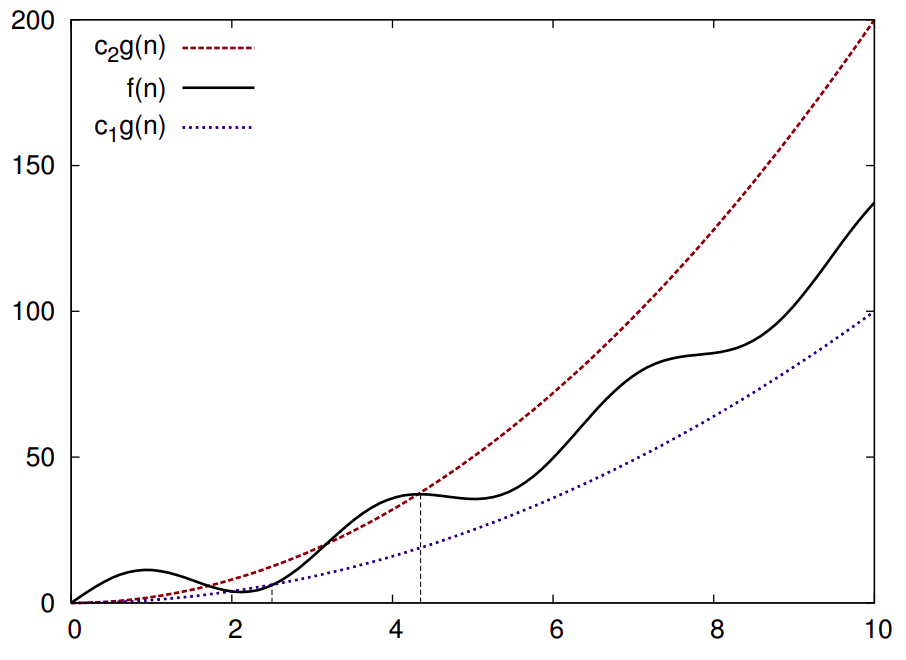
\includegraphics[width=\textwidth]{schema-theta.png}
    \caption{Curva di crescita di $f(n)=\Theta(g(n))$}
\end{figure}\noindent
Si noti come all'inizio la curva di $f(n)$ sembri disattendere le stime, ma
essendo \emph{stime asintotiche} esse valgono per $n\to+\infty$ e infatti,
superata una certa soglia, la curva di $f(n)$ rimane costantemente all'interno
della porzione di grafico disegnata dalle due curve di $g(n)$.

\begin{eg}[Verifica delle proprietà di un \bm{$O$}-grande]
    Si dimostri che $f(n)=10n^3+2n^2+7$ è un $O$-grande di
    $n^3$.

    \bigskip\noindent
    Riprendendo la definizione di \hyperref[def:4]{\emph{$O$}-grande}, dobbiamo
    dimostrare che:
    \[\exists\,c>0,\,\exists\,m\geq0:f(n)\leq c\cdot n^3\quad\forall\,n\geq m\]
    Procediamo:
    \[f(n)\begin{array}[t]{cll}
        =   &   10n^3+2n^2+7    & \\
        \leq&   10n^3+2n^3+7    & \qquad\forall\,n\geq1\\
        \leq&   10n^3+2n^3+n^3  & \qquad\forall\,n\geq\sqrt[3]{7}\\
        =   &   13n^3
    \end{array}\]
    A questo punto ci chiediamo se esistono un valore $c>0$ e un
    valore $m\geq 0$ tali che:
    \[13n^3\leq c\cdot n^3\]
    La risposta è banale poiché basta prendere $c\geq13$ e
    $m\geq1\geq\sqrt[3]{7}$, ad esempio, $m=2$.
\end{eg}
\begin{note}
    In questo esempio abbiamo potuto moltiplicare $2n^2$ per $n$
    e sostituire il $7$ con $n^3$, perché $n\geq0$. In realtà, nelle
    \emph{funzioni di costo} $n$ sarà sempre \emph{non negativo}, quindi lo
    potremo sempre fare.
\end{note}

\begin{eg}[Verifica delle proprietà di un \bm{$\Theta$}]
    Si dimostri che $f(n)=3n^2+7n$ è un $\Theta$ di $n^2$.

    \bigskip\noindent
    Procediamo verificando singolarmente i due estremi, inferiore e superiore.
    Iniziamo con lo studio del limite inferiore, cioè $\Omega$-grande. Ricordando
    la definizione di \hyperref[def:5]{\emph{$\Omega$}-grande} dobbiamo dimostrare
    che:
    \[\exists\,c_1>0,\,\exists\,m_1\geq0:f(n)\geq c_1\cdot n^2\quad\forall\,n\geq m_1\]
    Quindi:
    \[f(n)\begin{array}[t]{cll}
            =   &   3n^2+7n     & \\
            \geq&   3n^2        & \qquad\forall\,n\geq0\\
            \geq&   c_1\cdot n^2& \qquad\forall\,c_1\leq3\wedge\forall n\geq0
    \end{array}\]
    Pongo quindi $m_1=0$.

    \bigskip\noindent
    Passiamo ora allo studio del limite superiore. Come nell'esempio precedente
    dobbiamo dimostrare che:
    \[\exists\,c_2>0,\,\exists\,m_2\geq0:f(n)\leq c_2\cdot n^2\quad\forall\,n\geq m_2\]
    Quindi:
    \[f(n)\begin{array}[t]{cll}
        =   &   3n^2+7n     & \\
        \leq&   3n^2+7n^2   & \qquad\forall\,n\geq1\\
        =   &   10n^2       & \\
        \leq&   c_2\cdot n^2& \qquad\forall\,c_2\geq10\wedge\forall n\geq1
    \end{array}\]
    Pongo quindi $m_2=1$.

    \bigskip\noindent
    Torniamo ora al problema originario e riprendiamo la definizione di
    \hyperref[def:6]{$\Theta$}:
    \[\exists\,c_1>0,\,\exists\,c_2>0,\,\exists\,m\geq0:
    c_1\cdot g(n)\leq f(n)\leq c_2\cdot g(n)\quad\forall\,n\geq m\]
    Chiaramente, possiamo prendere $c_1=3$ e $c_2=10$, mentre,
    poiché l'ultima disequazione dev'essere vera $\forall\,n\geq m$,
    pongo $m=\max\{m_1,m_2\}=\max\{0,1\}=1$.

    \newpage\noindent
    Nel grafico seguente possiamo verificare la correttezza del
    nostri calcoli:
    \begin{figure}[h]
        \centering
        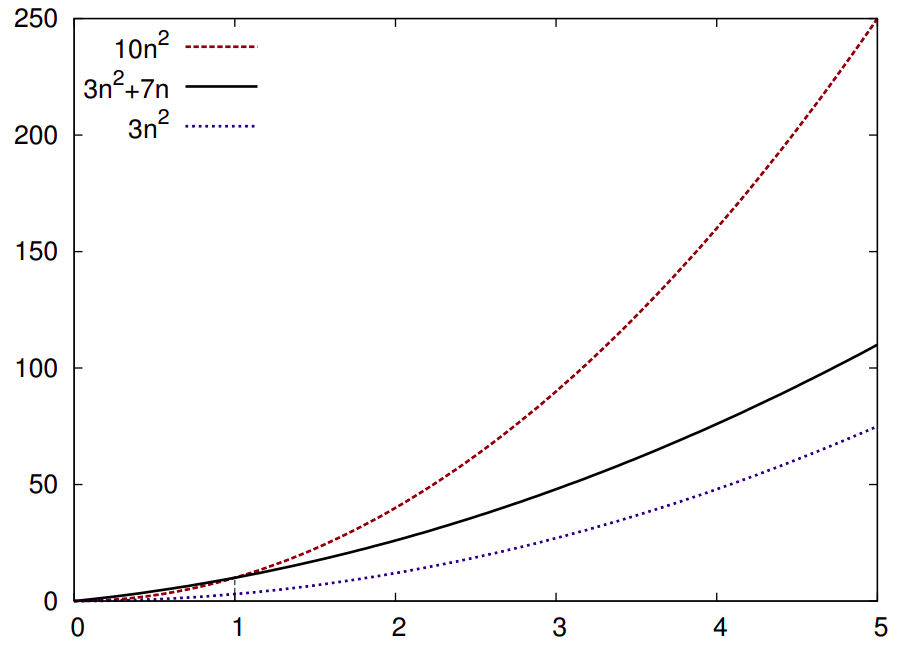
\includegraphics[scale=0.33]{schema-esempio-theta.png}
        \caption{Curva di $f(n)=3n^2+7n$}
    \end{figure}
\end{eg}

\section{Complessità degli algoritmi e dei problemi}
Solitamente, per risolvere uno stesso problema esistono una caterva di algoritmi
diversi e inevitabilmente alcuni sono più efficienti di altri. In che modo
lo studio della \emph{complessità} di questi \emph{algoritmi} può aiutarci a
capire la \emph{complessità del problema}?

Per rispondere a questa domanda sfruttiamo di nuovo la \emph{notazione
asintotica}.

\begin{definition}[Notazione $O$]
    Un problema ha complessità $O(f(n))$ se esiste almeno un algoritmo in grado
    di risolverlo che ha complessità $O(f(n))$.
\end{definition}

\begin{definition}[Notazione $\Omega$]
    Un problema ha complessità $\Omega(f(n))$ se tutti i possibili algoritmi che
    lo risolvono hanno complessità $\Omega(f(n))$.
\end{definition}

\paragraph{Notazione asintotica per gli algoritmi e per i problemi}
Nell'analisi della \emph{complessità degli algoritmi}, possiamo riassumere come
segue il significato delle \emph{notazioni asintotiche}:
\begin{itemize}
    \item $O(f(n))$: per tutti gli input $n$, l'algoritmo costa al più $f(n)$;
    \item $\Omega(f(n))$: per tutti gli input $n$, l'algoritmo costa almeno $f(n)$;
    \item $\Theta(f(n))$: per tutti gli input $n$, l'algoritmo costa $f(n)$;
\end{itemize}
Nell'analisi della \emph{complessità dei problemi}, vale invece:
\begin{itemize}
    \item $O(f(n))$: $O(f(n))$ è la complessità del miglior algoritmo in grado
    di risolvere il problema;
    \item $\Omega(f(n))$: vale se si riesce a dimostrare che nessun algoritmo
    può risolvere il problema in un tempo inferiore a $\Omega(f(n))$;
\end{itemize}
Se riusciamo a dimostrare che un problema ha complessità $O(f(n))$ e $\Omega(f(n))$,
un algoritmo con \emph{complessità} $\Theta(f(n))$ in grado di risolvere
quel problema, è il miglior algoritmo possibile.

\section[Ordinamento degli array in senso crescente]
{Ordinamento degli array in senso crescente\footnote{Il ragionamento è
analogo per ordinamenti in senso decrescente}}
Consideriamo ora tre diversi approcci al problema dell'ordinamento di array e
analizziamone la \emph{complessità}.

\subsection{Algoritmo Selection sort}
Questo algoritmo segue un approccio molto intuitivo: cerca il minimo tra tutti gli
elementi, lo ordina e poi ripete il tutto per i restanti elementi.

\begin{code}{Implementazione algoritmo Selection Sort}
\noindent\rmbreak SelectionSort(\bc{ITEM}[] A, \bc{int} n)\\
    \ind for (i = 1 to n - 1) do\\
        \indf\bc{int} min = min(A, i, n)\\
        \indf A[i] $\leftrightarrow$ A[min]\hfill\com{Scambia il minimo attuale e l'elemento $A[i]$}    
\end{code}
\vspace{-2\lineheight}
\begin{code}{Implementazione funzione min con indice di partenza arbitrario}
\noindent\rmbreak\ind\bc{int} min(\bc{ITEM}[] A, \bc{int} i, \bc{n})\\
    \bc{int} min = i\hfill\com{Posizione del minimo parziale}
    for (j = i + 1 to n) do\\
        \indf if (A[j] < A[min]) then\\
            \indff min = j\hfill\com{Nuovo minimo parziale}
    \ind return min
\end{code}\noindent
Quali sono le \emph{complessità} nei casi pessimo, medio e migliore?

\bigskip\noindent
Il caso pessimo è quello in cui l'array è ordinato in senso decrescente,
per cui ad ogni iterazione il minimo si trova nell'ultima posizione.
Il caso migliore è invece quello in cui l'array è già ordinato in senso crescente.
Nonostante questo, possiamo intuire che il costo dell'algoritmo non cambi, perché
in ogni caso si dovrà ricercare il minimo $n-1$ volte.

\bigskip\noindent
Provando a definire la \emph{funzione di costo} di questo algoritmo abbiamo:
\[\sum_{i=1}^{n-1}(n-i)=\sum_{i=1}^{n-1}i=\footnotemark\frac{n(n-1)}
{2}=n^2-\frac{n}{2}=O(n^2)\]
\footnotetext{\hyperlink{ser:1}{\emph{Formula di Gauss}}}
Questo vale per tutti i casi, quindi l'algoritmo \emph{insertion sort} ha un
costo $\Theta(n^2)$.

\subsection{Algoritmo Insertion sort}
Vediamo ora un approccio diverso al problema nel quale proviamo a prendere un
elemento per volta e a metterlo nella posizione giusta.

In particolare, ad ogni iterazione viene preso un valore e confrontato
progressivamente con i valori precedenti. Se viene trovato un valore minore di
quello preso, quest'ultimo viene salvato nella penultima cella
controllata.
\begin{code}{Implementazione algoritmo Insertion Sort}
\noindent\rmbreak\ind insertionSort(\bc{ITEM}[] A, \bc{int} n)\\
    for (i = 2 to n) do\\
        \indf \bc{ITEM} temp = A[i]\\
        \bc{int} j = i\\
        while (j > 1 and A[j - 1] > temp) do\\
            \indff A[j] = A[j - 1]\\
            j = j - 1\\
        \indf A[j] = temp
\end{code}\noindent
Cosa succede nei casi pessimo, medio e migliore?

\bigskip\noindent
Come prima, il caso pessimo è quello in cui l'array è ordinato in senso
contrario. In una situazione del genere, per ogni $i$ devono essere fatti $i-1$
confronti. Si ha quindi una funzione di questo tipo:
\[\sum_{i=2}^n(i-1)=\sum_{i=1}^{n-1}(n-i)=O(n^2)\]
Nel caso migliore invece, il vettore è già ordinato nel senso corretto col
risultato che ad ogni iterazione il controllo \texttt{A[j-1] > temp} è sempre
falso e quindi la funzione di costo è:
\[\sum_{i=2}^n1=n-2=O(n)\]

\hypertarget{sec:merge_sort}{\subsection{Algoritmo Merge sort}}
Questo algoritmo è basato sulla tecnica del \emph{divide-et-impera}, cioè procede
suddividendo l'array in due metà che vengono poi ordinate separatamente e quindi
ricombinate per ottenere l'array di partenza ordinato.

Come sarà facile intuire, questo algoritmo sfrutta la ricorsione per suddividere
l'array in due componenti e una qualche funzione per l'unione dei due sottoarray
ordinati.

\begin{code}{Implementazione algoritmo Merge sort}
\noindent\rmbreak\ind mergeSort(\bc{ITEM}[] A, \bc{int} first, \bc{int} last)\\
    if (first < last) then\\
        \indf\bc{int} mid = $\lfloor$(first + last) / 2$\rfloor$\\
        mergeSort(A, first, mid)\hfill\com{Ordina la parte sinistra}
        mergeSort(A, mid + 1, last)\hfill\com{Ordina la parte destra}
        merge(A, first, last, mid)\hfill\com{Combina i due sottoarray ordinati}
\end{code}\noindent
Nella funzione \texttt{merge} ipotizziamo di avere a disposizione un array di
appoggio $B$ nel quale andiamo ad inserire, in modo ordinato, i valori dei due
sottoarray di $A$. Una volta riempito, tutti i valori di $B$ vengono ricopiati
di nuovo su $A$.
\begin{code}{Implementazione funzione merge}
\noindent\rmbreak\ind merge(\bc{ITEM}[] A, \bc{int} first, \bc{int} last, \bc{int} mid)\\
    \bc{int} i, j, k, h\\
    i = first\\
    j = mid + 1\\
    k = first\hfill\com{Indice delle posizioni nell'array di appoggio}
    while (i $\leq$ mid and j $\leq$ last) do\hfill\com{Popolamento di $B$}
        \indf if (A[i] $\leq$ A[j]) then\\
            \indff B[k] = A[i]\\
            i = i + 1\\
        \indf else\\
            \indff B[k] = A[j]\\
            j = j + 1\\
        \indf k = k + 1\\
    \ind j = last\\
    for (h = mid downto i) do\\
        \indf A[j] = A[h]\\
        \indf j = j - 1\\
    \ind for (j = first to k - 1) do\hfill\com{Copia di $B$ su $A$}
        \indf A[j] = B[j]
\end{code}\noindent
Qual è la complessità del \emph{merge sort}?

\bigskip\noindent
Studiamo per prima la sola funzione \emph{merge}.
Nel ciclo \texttt{while} e nel secondo ciclo \texttt{for}, vengono fatte $n$
assegnazioni, dunque la funzione ha complessità $O(n)$.

Passando a considerare l'algoritmo nel suo insieme vediamo che l'array viene
diviso in due metà e poi viene invocata \emph{merge}. Ciò significa
che se si tracciano i partizionamenti dell'array durante l'esecuzione
dell'algoritmo, si ottiene un albero binario di altezza $k=\log n$\footnote{Per
semplicità ipotizziamo che il numero di elementi dell'array sia una potenza di 2}
nel quale, ad ogni livello $i$, la funzione $merge$ viene invocata $2^i$ volte.

\begin{figure}[hb]
\centering
\begin{tikzpicture}[node distance={20mm},main/.style={draw, circle, scale=0.95}]
	\node[main] (1) {$n$};

    \node[] (2) [below of=1] {$+$};
    \node[main] (3) [left of=2, xshift=-10mm] {$\frac{n}{2}$};
    \node[main] (4) [right of=2, xshift=10mm] {$\frac{n}{2}$};

    \node[] (5) [below of=3] {$+$};
    \node[main] (6) [left of=5, xshift=5mm] {$\frac{n}{2^2}$};
    \node[main] (7) [right of=5, xshift=-5mm] {$\frac{n}{2^2}$};

    \node[] (8) [below of=2] {$+$};

    \node[] (9) [below of=4] {$+$};
    \node[main] (10) [left of=9, xshift=5mm] {$\frac{n}{2^2}$};
    \node[main] (11) [right of=9, xshift=-5mm] {$\frac{n}{2^2}$};

    \node[] (12) [below of=6, xshift=-7.5mm] {$\vdots$};
    \node[] (13) [below of=6, xshift=7.5mm] {$\vdots$};

    \node[] (14) [below of=7, xshift=-7.5mm] {$\vdots$};
    \node[] (15) [below of=7, xshift=7.5mm] {$\vdots$};

    \node[] (16) [below of=10, xshift=-7.5mm] {$\vdots$};
    \node[] (17) [below of=10, xshift=7.5mm] {$\vdots$};

    \node[] (18) [below of=11, xshift=-7.5mm] {$\vdots$};
    \node[] (19) [below of=11, xshift=7.5mm] {$\vdots$};
    
    \node[] (20) [below of=12] {$+$};
    \node[main] (21) [below of=12, xshift=-7.5mm, yshift=-1mm] {$\frac{n}{2^k}$};
    \node[main] (22) [below of=12, xshift=7.5mm, yshift=-1mm] {$\frac{n}{2^k}$};

    \node[] (23) [below of=8] {};
    \node[] (24) [below of=23] {$\cdots$};

    \node[] (25) [below of=14] {$+$};
    \node[] (26) [below of=17] {$+$};

    \node[] (27) [below of=19] {$+$};
    \node[main] (28) [below of=19, xshift=-7.5mm, yshift=-1mm] {$\frac{n}{2^k}$};
    \node[main] (29) [below of=19, xshift=7.5mm, yshift=-1mm] {$\frac{n}{2^k}$};

    \node[] (30) [right of=29, xshift=7.5mm]
    {\hspace{0.8cm}\begin{tabular}{rl}
        $O(n)$ & $k=\log n$
    \end{tabular}};
    \node[] (31) [above of=30, yshift=-10mm] {$+$};
    \node[] (32) [above of=31, yshift=-10mm] {$\vdots$};
    \node[] (33) [above of=32, yshift=-10mm] {$+$};
    \node[] (34) [above of=33, yshift=-10mm]
    {\begin{tabular}{rl}
        $O(n)$ & $k=2$
    \end{tabular}};
    \node[] (35) [above of=34, yshift=-10mm] {$+$};
    \node[] (35) [above of=35, yshift=-10mm]
    {\begin{tabular}{rl}
        $O(n)$ & $k=1$
    \end{tabular}};
    \node[] (36) [above of=35, yshift=-10mm] {$+$};
    \node[] (37) [above of=36, yshift=-10mm]
    {\begin{tabular}{rl}
        $O(n)$ & $k=0$
    \end{tabular}};

    \draw (1) -- (3);
    \draw (1) -- (4);
    \draw (3) -- (6);
    \draw (3) -- (7);
    \draw (4) -- (10);
    \draw (4) -- (11);
    \draw (6) -- (12);
    \draw (6) -- (12);
    \draw (6) -- (13);
    \draw (7) -- (14);
    \draw (7) -- (15);
    \draw (10) -- (16);
    \draw (10) -- (17);
    \draw (11) -- (18);
    \draw (11) -- (19);
    \draw (12) -- (21);
    \draw (12) -- (22);
    \draw (19) -- (28);
    \draw (19) -- (29);
\end{tikzpicture}
\caption{Schema d'esecuzione del \emph{Merge sort}}
\end{figure}\noindent
Ogni livello ha un costo $O(n)$, quindi, essendoci $k=\log n$ livelli, il costo
dell'algoritmo è $O(n\log n)$. Possiamo verificare il nostro risultato
svolgendo direttamente i calcoli:
\[O\left(\sum_{i=0}^k2^i\cdot\frac{n}{2^i}\right)=O\left(\sum_{i=0}^kn\right)=
O(k\cdot n)=O(n\log n)\]
Nel primo passaggio, l'argomento della sommatoria è quello perché per ogni livello
sommiamo il costo necessario ad eseguire il merge su ogni sottoarray di dimensione
$\frac{n}{2^i}$ (e.g. il sottoarray al livello 1 avrà dimensione $\frac{n}{2^1}$),
ma consideriamo anche la numerosità dei sottoarray: $2^i$ per ogni livello $i$.

Ragionando anche sulla \emph{funzione di costo} constatiamo che, poiché ad ogni
livello vengono effettuate due invocazioni della \texttt{mergeSort} e
un'invocazione della \texttt{merge}, che ha costo $O(n)$, vale la seguente:
\[T(n)=\begin{cases}
    2T(n/2)+dn & n>1\\
    c & n=1\\
\end{cases}\]
\chapter{Notazione asintotica}
Nel precedente capitolo abbiamo introdotto velocemente la \emph{notazione
asintotica}, ma ora la riprendiamo per approfondirne le caratteristiche e 
iniziamo con l'esplicitare una regola generale che finora abbiamo sfruttato
senza pensarci troppo.

\begin{definition}[Regola generale per le espressioni polinomiali]
    Per ogni espressione polinomiale di grado $k$ del tipo
    \[\begin{array}{rc}
        f(n)=a_k\cdot n^k+a_{k-1}\cdot n^{k-1}+\dots+a_1\cdot n+a_0 & a_k>0
    \end{array}\]
    vale:
    \[f(n)=\Theta(n^k)\]
\end{definition}
\begin{proof}[Dimostrazione]
    La condizione necessaria per poter dire che $f(n)=\Theta(n^k)$ è:
    \[\begin{array}{rcl}
        f(n)=O(n^k) & \wedge & f(n)=\Omega(n^k)
    \end{array}\]
    Iniziamo quindi con la verifica del \emph{limite superiore}, ovvero dimostriamo
    che vale la seguente:
    \[\exists\,c>0,\,\exists\,m\geq 0:f(n)\leq c\cdot n^k\quad\forall\,n\geq m\]
    Procediamo:
    \[f(n)\begin{array}[t]{clr}
        = & a_k\cdot n^k+a_{k-1}\cdot n^{k-1}+\dots+a_1\cdot n+a_0 & \\
        \leq & a_k\cdot n^k+|a_{k-1}|\cdot n^{k-1}+\dots+|a_1|\cdot n+|a_0| & \\
        \leq & a_k\cdot n^k+|a_{k-1}|\cdot n^k+\dots+|a_1|\cdot n^k+|a_0|\cdot n^k & \forall\,n\geq 1\\
        = & (a_k+|a_{k-1}|+\dots+|a_1|+|a_0|)\cdot n^k & \\
        \leq & c\cdot k^n
    \end{array}\]
    L'ultima disequazione è vera per:
    \[\begin{array}{rcl}
        c\geq(a_k+|a_{k-1}|+\dots+|a_1|+|a_0|) & \wedge & m=1
    \end{array}\]

    \bigskip\noindent
    Ora passiamo alla verifica del \emph{limite inferiore} e quindi dimostriamo
    che vale anche la seguente:
    \[\exists\,d>0,\,\exists\,m\geq 0:f(n)\geq d\cdot n^k\quad\forall\,n\geq m\]
    Procediamo:
    \[f(n)\begin{array}[t]{clr}
        = & a_k\cdot n^k+a_{k-1}\cdot n^{k-1}+\dots+a_1\cdot n+a_0 & \\
        \geq & a_k\cdot n^k-|a_{k-1}|\cdot n^{k-1}-\dots-|a_1|\cdot n-|a_0| & \\
        \geq & a_k\cdot n^k-|a_{k-1}|\cdot n^{k-1}-\dots-|a_1|\cdot n^{k-1}-|a_0|\cdot n^{k-1} & \forall\,n\geq 1\\
        \geq & d\cdot n^k
    \end{array}\]
    L'ultima disequazione è vera per:
    \[d\leq a_k-\frac{|a_{k-1|}}{n}-\frac{|a_{k-2}|}{n}-\dots-\frac{|a_1|}{n}-
    \frac{|a_0|}{n}\]
    Poiché $d>0$, anche il termine destro della disequazione dev'essere $>0$,
    e quindi deve valere:
    \[\begin{array}{rcl}
        a_k-\frac{|a_{k-1|}}{n}-\frac{|a_{k-2}|}{n}-\dots-\frac{|a_1|}{n}-
    \frac{|a_0|}{n} > 0 & \Leftrightarrow & n\geq\frac{|a_{k-1}|+\dots+|a_1|+|a_0|}
    {a_k}=m
    \end{array}\]
\end{proof}

\section{Proprietà della notazione asintotica}
\begin{definition}[Proprietà di dualità]
    Per ogni coppia di funzioni di costo $f(n)$ e $g(n)$ vale:
    \[f(n)=O(g(n))\Leftrightarrow g(n)=\Omega(f(n))\]
\end{definition}
\begin{proof}[Dimostrazione]
    \[f(n)=O(g(n))\begin{array}[t]{cll}
        \Leftrightarrow & f(n)\leq c\cdot g(n) & \forall\,n\geq m\\
        \Leftrightarrow & g(n)\geq\frac{1}{c}\cdot f(n) & \forall\,n\geq m\\
        \Leftrightarrow & g(n)\geq c'\cdot f(n) & \forall\,n\geq m,\,c'=\frac{1}{c}\\
        \Leftrightarrow & g(n)=\Omega(f(n)) &
    \end{array}\]
\end{proof}\noindent
Questa proprietà stabilisce che se $f(n)$ è un $O(g(n))$, allora $g(n)$ è un
$\Omega(f(n))$.

\begin{definition}[Proprietà di eliminazione delle costanti]
    Per ogni funzione di costo $f(n)$ vale:
    \[f(n)=O(g(n))\Leftrightarrow a\cdot f(n)=O(g(n))\quad\forall\, a>0\]
    \[f(n)=\Omega(g(n))\Leftrightarrow a\cdot f(n)=\Omega(g(n))\quad\forall\, a>0\]
\end{definition}
\begin{proof}[Dimostrazione]
    \[f(n)=O(g(n))\begin{array}[t]{cll}
        \Leftrightarrow & f(n)\leq c\cdot g(n) & \forall\,n\geq m\\
        \Leftrightarrow & a\cdot f(n)\leq a\cdot c\cdot g(n) & \forall\,n\geq m,\,\forall\,a>0\\
        \Leftrightarrow & a\cdot f(n)\leq c'\cdot g(n) & \forall n\geq m,\,c'=a\cdot c>0\\
        \Leftrightarrow & a\cdot f(n)=O(g(n)) &
    \end{array}\]
\end{proof}
\begin{note}
    La dimostrazione è analoga per $\Omega(g(n))$.
\end{note}\noindent
Questa proprietà permette di ignorare le costanti moltiplicative per le
\emph{funzioni di costo}.

\begin{definition}[Proprietà di massimo costo]
    Per ogni coppia di funzioni di costo $f_1(n)$ e $f_2(n)$ vale:
    \[f_1(n)=O(g_1(n)),\,f_2(n)=O(g_2(n))\Rightarrow f_1(n)+f_2(n)=
    O(\max\{g_1(n),\,g_2(n)\})\]
    \[f_1(n)=\Omega(g_1(n)),\,f_2(n)=\Omega(g_2(n))\Rightarrow f_1(n)+f_2(n)=
    \Omega(\max\{g_1(n),\,g_2(n)\})\]
\end{definition}
\begin{proof}[Dimostrazione]
    \[\begin{array}{rc}
        f_1(n)=O(g_1(n))\wedge f_2(n)=O(g_2(n)) & \Rightarrow\\
        f_1(n)\leq c_1\cdot g_1(n)\wedge f_2(n)\leq c_2\cdot g_2(n) & \Rightarrow\\
        f_1(n)+f_2(n)\leq c_1\cdot g_1(n)+c_2\cdot g_2(n) & \Rightarrow\\
        f_1(n)+f_2(n)\leq\max\{c_1,\,c_2\}\cdot(2\max\{g_1(n),\,g_2(n)\}) & \Rightarrow\\
        f_1(n)+f_2(n)=O(\max\{g_1(n),\,g_2(n)\})
    \end{array}\]
\end{proof}
\begin{note}
    La dimostrazione è analoga per $f_1(n)+f_2(n)=\Omega(\max\{g_1(n),\,g_2(n)\})$.
\end{note}\noindent
Questa proprietà stabilisce, che nel caso in cui si vada a sommare più \emph{funzioni
di costo} (e.g. sequenze di algoritmi), si può considerare solo la funzione di
costo maggiore.

\begin{definition}[Proprietà del prodotto dei costi]
    Per ogni coppia di funzioni di costo $f_1(n)$ e $f_2(n)$ vale:
    \[f_1(n)=O(g_1(n)),\,f_2(n)=O(g_2(n))\Rightarrow f_1(n)\cdot f_2(n)=
    O(g_1(n)\cdot g_2(n))\]
    \[f_1(n)=\Omega(g_1(n)),\,f_2(n)=\Omega(g_2(n))\Rightarrow f_1(n)\cdot f_2(n)=
    \Omega(g_1(n)\cdot g_2(n))\]
\end{definition}
\begin{proof}[Dimostrazione]
    \[\begin{array}{rc}
        f_1(n)=O(g_1(n))\wedge f_2(n)=O(g_2(n)) & \Rightarrow\\
        f_1(n)\leq c_1\cdot g_1(n)\wedge f_2(n)\leq c_2\cdot g_2(n) & \Rightarrow\\
        f_1(n)\cdot f_2(n)\leq c_1\cdot c_2\cdot g_1(n)\cdot g_2(n) & \Rightarrow\\
        f_1(n)\cdot f_2(n)=O(g_1(n)\cdot g_2(n))
    \end{array}\]
\end{proof}
\begin{note}
    La dimostrazione è analoga per $f_1(n)\cdot f_2(n)=\Omega(g_1(n)\cdot g_2(n))$.
\end{note}\noindent
Questa proprietà stabilisce che nel caso in cui si vada a moltiplicare tra loro più
\emph{funzioni di costo} (e.g. cicli annidati), il costo totale è proprio il
prodotto dei costi delle singole funzioni.

\begin{definition}[Proprietà di simmetria]
    Per ogni coppia di funzioni di costo $f(n)$ e $g(n)$ vale:
    \[f(n)=\Theta(g(n))\Leftrightarrow g(n)=\Theta(f(n))\]
\end{definition}
\begin{proof}[Dimostrazione]
    Grazie alla \emph{proprietà di dualità} vale:
    \[\begin{array}{rcccl}
        f(n)=\Theta(g(n)) & \Rightarrow & f(n)=O(g(n)) & \Rightarrow & g(n)=\Omega(f(n))\\
        f(n)=\Theta(g(n)) & \Rightarrow & f(n)=\Omega(g(n)) & \Rightarrow & g(n)=O(f(n))
    \end{array}\]
\end{proof}\noindent
Questa proprietà stabilisce che se $f(n)$ è un $\Theta(g(n))$ allora anche $g(n)$
è un $\Theta(f(n))$.

\begin{definition}[Proprietà di transitività]
    Prese tre funzioni di costo $f(n)$, $g(n)$ e $h(n)$ tali che:
    \[\begin{array}{lcr}
        f(n)=O(g(n)) & \wedge & g(n)=O(h(n))
    \end{array}\]
    vale:
    \[f(n)=O(h(n))\]
\end{definition}
\begin{proof}[Dimostrazione]
    \[\begin{array}{rc}
        f(n)=O(g(n))\wedge g(n)=O(h(n)) & \Rightarrow\\
        f(n)\leq c_1\cdot g(n)\wedge g(n)\leq c_2\cdot h(n) & \Rightarrow\\
        f(n)\leq c_2\cdot h(n) & \Rightarrow\\
        f(n)=O(h(n))
    \end{array}\]
\end{proof}

\section{Altre notazioni}
\begin{definition}[Notazione $o$]
    Sia $g(n)$ una funzione di costo. Si indica con $o(g(n))$ l'insieme delle
    funzioni di costo tali per cui:
    \[\forall\,c,\,\exists\,m:f(n)<c\cdot g(n)\quad\forall\,n\geq m\]
\end{definition}\noindent
Le funzioni $f(n)$ che rispettano questa disuguaglianza sono dette essere
\emph{$o$-piccoli} di $g(n)$ e si scrive in simboli $f(n)=o(g(n))$.

\begin{definition}[Notazione $\omega$]
    Sia $g(n)$ una funzione di costo. Si indica con $\omega(g(n))$ l'insieme
    delle funzioni di costo tali per cui:
    \[\forall\,c,\,\exists\,m:f(n)>c\cdot g(n)\quad\forall\,n\geq m\]
\end{definition}\noindent
Le funzioni $f(n)$ che rispettano questa disuguaglianza sono dette essere
\emph{$\omega$-piccoli} di $g(n)$ e si scrive in simboli $f(n)=\omega(g(n))$.

\paragraph{Osservazioni}
Date due \emph{funzioni di costo} $f(n)$ e $g(n)$ possiamo fare le seguenti
affermazioni:
\[\renewcommand{\arraystretch}{1.3} 
\begin{array}{rcl}
    \lim\limits_{n\to+\infty}\frac{f(n)}{g(n)}=0 & \Rightarrow & f(n)=o(g(n))\\
    \lim\limits_{n\to+\infty}\frac{f(n)}{g(n)}=c\neq0 & \Rightarrow & f(n)=\Theta(g(n))\\
    \lim\limits_{n\to+\infty}\frac{f(n)}{g(n)}=+\infty & \Rightarrow & f(n)=\omega(g(n))
\end{array}\]
Si noti anche che:
\[\begin{array}{rcl}
    f(n)=o(g(n)) & \Rightarrow & f(n)=O(g(n))\\
    f(n)=\omega(g(n)) & \Rightarrow & f(n)=\Omega(g(n))
\end{array}\]

\section{Classificazione delle funzioni di costo}
Giunti a questo punto possiamo definire un ordinamento per le principali
\emph{funzioni di costo}:

\begin{definition}[Ordinamento delle funzioni di costo]
    Per ogni $r<s$, $h<k$ e $a<b$ vale:
    \[O(1)\subset O(\log^rn)\subset O(\log^sn)\subset O(n^h)\subset
    O(n^h\log^rn)\]
    \[\subset O(n^h\log^sn)\subset O(n^k)\subset O(a^n)\subset O(b^n)\]
\end{definition}
\chapter{Funzioni di ricorrenza}
Quando  si calcola la \emph{complessità} di un algoritmo ricorsivo, questa viene
espressa tramite un'\emph{equazione} o una \emph{funzione di ricorrenza}, ovvero
una formula matematica definita in maniera ricorsiva.

Un esempio di \emph{equazione di ricorrenza} è quella che descrive il costo
dell'algoritmo \hyperlink{sec:merge_sort}{\emph{Merge sort}}:
\[T(n)\footnote{Questa descrive il caso generale, mentre la precedente
si basava sull'ipotesi di array di dimensione $2^i$ con $i\in\mathbb{N}$}
=\begin{cases}
    T(\lfloor n/2\rfloor) + T(\lceil n/2\rceil) + \Theta(n) & n>1\\
    \Theta(1) & n\leq 1
\end{cases}\]
Il nostro obiettivo è ottenere, quando possibile, una \emph{formula}, o
\emph{forma chiusa}, che rappresenti la \emph{classe di complessità} della
funzione. Nell'esempio del \emph{Merge sort} la \emph{formula chiusa} è:
\[T(n)=\Theta(n\log n)\]

\bigskip\noindent In realtà, le \emph{equazioni di ricorrenza} possono essere
usate anche per risolvere problemi. Vediamone un esempio:

\begin{problem}[Applicazione delle funzioni di ricorrenza nella risoluzione di problemi]
    Un bambino scende una scala composta da $n$ scalini. Ad ogni passo,
    può decidere di fare $1,2,3,4$ scalini alla volta. Determinare in quanti
    modi diversi può scendere le scale.
    
    Ad esempio, se $n=7$, alcuni dei modi possibili sono i seguenti:
    \begin{itemize}
        \item 1,1,1,1,1,1,1;
        \item 1,2,4;
        \item 4,2,1;
        \item 2,2,2,1;
        \item 1,2,2,1,1;
    \end{itemize}

    \newpage
    \paragraph{Soluzione} Sia $M(n)$ il numero di modi in cui è possibile scegliere
    $n$ scalini. $M(n)$ può essere espresso come segue:
    \[M(n)=\begin{cases}
        0 & n<0\\
        1 & n=0\\
        \sum_{k=1}^4M(n-k) & n>0
    \end{cases}\]
\end{problem}\noindent
Questa \emph{ricorrenza} può poi essere trasformata in un algoritmo\footnote{Il
risultato sono i \emph{numeri di Tetranacci}: $1,1,2,4,8,15,29,56,108,208, 401,
773,1490,2872, 5536,\dots$.} tramite \emph{ricorsione} o \emph{programmazione
dinamica}.

\section{Studio delle equazioni di ricorrenza}
Vediamo di seguito alcuni modi per analizzare le \emph{funzioni di ricorrenza}
e ricavarne la \emph{forma chiusa}.

\subsection{Metodo dell'albero di ricorsione}
Il \emph{metodo dell'albero di ricorsione} (o per \emph{livelli}) prevede che la
\emph{ricorrenza} venga \q{srotolata} in un albero i cui nodi rappresentano il
costo ai vari livelli della ricorsione.

\begin{eg}[Esempio semplice di analisi con albero di ricorsione]
    Sia $T(n)$ la seguente funzione di ricorrenza:
    \[T(n)=\begin{cases}
        T(n/2)+b & n>1\\
        c & n\leq1
    \end{cases}\]

    \bigskip\noindent
    Ipotizziamo, per semplicità, che $n=2^k$, quindi proviamo a
    risolvere $T(n)=T(2^k)$:
    \[T(n)\begin{array}[t]{cl}
        = & b + T(n/2)\\
        = & b + b + T(n/4)\\
        = & b + b + b + T(n/8)\\
        = & \dots\\
        = & \underbrace{b + \dots + b}_{\log n} + T(1)\\
        = & b\cdot\log n + c
    \end{array}\]
    Quindi, $T(n)=b\cdot\log k + c=\Theta(\log n)$.
\end{eg}

\begin{eg}[Utilizzo delle serie matematiche nel processo di semplificazione]
    Sia $T(n)$ la seguente funzione di ricorrenza:
    \[T(n)=\begin{cases}
        4T(n/2)+n & n>1\\
        1 & n\leq1
    \end{cases}\]

    \newpage\noindent
    Ipotizziamo sempre $n=2^k$:
    \[T(n)\begin{array}[t]{cl}
        = & n + 4T(n/2)\\
        = & n + 4(n/2) + 16T(n/4)\\
        = & n + 2n + 16(n/4) + 64T(n/8)\\
        = & \dots\\
        = & n + 2n + 4n + 8n + \dots + 2^{\log(n)-1}n + 4^{\log n}T(1)\\
        = & \left(\sum_{i=0}^{\log(n)-1}2^i\right)\cdot n+4^{\log n}
    \end{array}\]
    A questo punto, possiamo sfruttare la \hyperlink{ser:2}{serie geometrica
    finita} e riscrivere la funzione come:
    \[T(n)\begin{array}[t]{cll}
        = & \left(\sum_{i=0}^{\log(n)-1}2^i\right)\cdot n+4^{\log n}\\
        = & \left(\frac{2^{\log n}-1}{2 - 1}\right)\cdot n + 4^{\log n} & \quad\hyperlink{ser:2}{\text{Serie geometrica finita}}\\
        = & (2^{\log n}-1)\cdot n+4^{\log n}\\
        = & (n^{\log 2}-1)\cdot n+n^{\log 4} & \quad\hyperlink{log:12}{\text{Teorema di scambio base-argomento}}\\
        = & (n^1-1)\cdot n+n^2\\
        = & (n-1)\cdot n+n^2\\
        = & n^2 - n + n^2\\
        = & 2n^2 - n
    \end{array}\]
    Da qui è evidente che $T(n)=\Theta(n^2)$.
\end{eg}

\begin{eg}[Utilizzo di una tabella dei costi]
    Sia $T(n)$ la seguente funzione di ricorrenza:
    \[t(n)=\begin{cases}
        4T(n/2)+n^3 & n>1\\
        1 & n\leq1
    \end{cases}\]

    \bigskip\noindent
    Proviamo ad analizzare l'albero delle chiamate per i primi 3 livelli:
    \begin{center}
    \resizebox{1\hsize}{!}{
    \LARGE
    $\begin{array}{c}
        n^3\\\\
        \overbrace{\begin{array}{cccc}
            \begin{array}{c}
                \left(\frac{n}{2}\right)^3\\\\
                \overbrace{\begin{array}{cccc}
                    \left(\frac{n}{4}\right)^3 & \left(\frac{n}{4}\right)^3 &
                    \left(\frac{n}{4}\right)^3 & \left(\frac{n}{4}\right)^3\\
                \end{array}}
            \end{array} &
            \begin{array}{c}
                \left(\frac{n}{2}\right)^3\\\\
                \overbrace{\begin{array}{cccc}
                    \left(\frac{n}{4}\right)^3 & \left(\frac{n}{4}\right)^3 &
                    \left(\frac{n}{4}\right)^3 & \left(\frac{n}{4}\right)^3\\
                \end{array}}
            \end{array} &
            \begin{array}{c}
                \left(\frac{n}{2}\right)^3\\\\
                \overbrace{\begin{array}{cccc}
                    \left(\frac{n}{4}\right)^3 & \left(\frac{n}{4}\right)^3 &
                    \left(\frac{n}{4}\right)^3 & \left(\frac{n}{4}\right)^3\\
                \end{array}}
            \end{array} &
            \begin{array}{c}
                \left(\frac{n}{2}\right)^3\\\\
                \overbrace{\begin{array}{cccc}
                    \left(\frac{n}{4}\right)^3 & \left(\frac{n}{4}\right)^3 &
                    \left(\frac{n}{4}\right)^3 & \left(\frac{n}{4}\right)^3\\
                \end{array}}
            \end{array}
        \end{array}}\\
    \end{array}$}
    \end{center}
    È chiaro che con una funzione di questo tipo, non è possibile procedere in
    questo modo. Una strategia migliore è quella di usare una tabella come la
    seguente.
    \begin{table}[ht]
    \renewcommand{\arraystretch}{1.2}
    \centering
    \begin{tabular}{|c|c|c|c|c|}
        \hline
        \textbf{Livello} & \textbf{Dim. input} & \textbf{Costo per chiamata} & \textbf{N. chiamate} & \textbf{Costo livello}\\
        \hline
        $0$ & $n$ & $n^3$ & $1$ & $n^3$\\
        \hline
        $1$ & $n/2$ & $(n/2)^3$ & $4$ & $4(n/2)^3$\\
        \hline
        $2$ & $n/4$ & $(n/4)^3$ & $16$ & $16(n/4)^3$\\
        \hline
        \dots & \dots & \dots & \dots & \dots\\
        \hline
        $i$ & $n/2^i$ & $(n/2^i)^3$ & $4^i$ & $4^i(n/2^i)^3$\\
        \hline
        \dots & \dots & \dots & \dots & \dots\\
        \hline
        $\log(n)-1$ & $n/2^{\log(n)-1}$ & $\left(n/2^{\log(n)-1}\right)$ & $4^{\log(n)-1}$ & $4^{\log(n))-1}\left(n/2^{\log(n)-1}\right)^3$\\
        \hline
        $\log n$ & $1$ & $T(1)$ & $4^{\log n}$ & $4^{\log n}$\\
        \hline
    \end{tabular}
    \end{table}\newpage\noindent
    Ora, il costo totale è dato dalla somma del costo di ogni livello. Vale
    quindi:
    \[T(n)\begin{array}[t]{cll}
        = & \sum_{i=0}^{\log(n)-1}\left(4^i\left(n/2^i\right)^3\right)+4^{\log n}\\
        = & \left(\sum_{i=0}^{\log(n)-1}\frac{4^i}{2^{3i}}\right)\cdot n^3 + 4^{\log n}\\
        = & \left(\sum_{i=0}^{\log(n)-1}\frac{2^{2i}}{2^{3i}}\right)\cdot n^3 + 4^{\log n}\\
        = & \left(\sum_{i=0}^{\log(n)-1}\left(\frac{1}{2}\right)^i\right)\cdot n^3 + 4^{\log n}\\
        = & \left(\sum_{i=0}^{\log(n)-1}\left(\frac{1}{2}\right)^i\right)\cdot n^3 + n^{\log 4} &
        \quad\hyperlink{log:12}{\text{Teorema di scambio base-argomento}}\\
        = & \left(\sum_{i=0}^{\log(n)-1}\left(\frac{1}{2}\right)^i\right)\cdot n^3 + n^2\\
        \leq & \left(\sum_{i=0}^{+\infty}\left(\frac{1}{2}\right)^i\right)\cdot n^3 + n^2 &
        \quad\text{Estensione ad infinito della sommatoria}\\
    \end{array}\]
    Giunti a questo punto abbiamo:
    \[T(n)\leq\left(\sum_{i=0}^{+\infty}\left(\frac{1}{2}\right)^i\right)\cdot n^3 + n^2\]
    Tuttavia, possiamo riconoscere nella sommatoria la \hyperlink{ser:4}
    {serie geometrica infinita decrescente} e riscrivere $T(n)$ come:
    \[T(n)\begin{array}[t]{cl}
        \leq & \frac{1}{1-\frac{1}{2}}n^3+n^2\\
        \leq & 2n^3+n^2
    \end{array}\]
    Abbiamo quindi dimostrato che $T(n)=O(n^3)$, tuttavia, poiché $T(n)\geq n^3$,
    possiamo anche affermare che $T(n)=\Omega(n^3)$, quindi $T(n)=\Theta(n^3)$.
\end{eg}

\begin{note}
    Abbiamo indicato $n^3$ come costo della prima chiamata perché di sicuro
    lo si dovrà pagare, ma in realtà il vero costo avrebbe dovuto essere
    $c\cdot n^3$ per qualche $c>0$. Abbiamo rimosso $c$ per semplicità, ma
    grazie alla \hyperlink{prop:elimcost}{\emph{Proprietà di eliminazione
    delle costanti}} sappiamo che considerarlo non sarebbe comunque servito.
\end{note}

\begin{eg}[Ulteriore esempio di utilizzo di una tabella dei costi]
    Sia $T(n)$ la seguente funzione di ricorrenza:
    \[T(n)=\begin{cases}
        4T(n/2)+n^2 & n>1\\
        1 & n\leq1
    \end{cases}\]

    \bigskip\noindent
    Procediamo utilizzando una tabella come quella di prima.

    \begin{table}[ht!]
        \renewcommand{\arraystretch}{1.2}
        \centering
        \begin{tabular}{|c|c|c|c|c|}
            \hline
            \textbf{Livello} & \textbf{Dim. input} & \textbf{Costo per chiamata} & \textbf{N. chiamate} & \textbf{Costo livello}\\
            \hline
            $0$ & $n$ & $n^2$ & $1$ & $n^2$\\
            \hline
            $1$ & $n/2$ & $(n/2)^2$ & $4$ & $4(n/2)^2$\\
            \hline
            $2$ & $n/4$ & $(n/4)^2$ & $16$ & $16(n/4)^2$\\
            \hline
            \dots & \dots & \dots & \dots & \dots\\
            \hline
            $i$ & $n/2^i$ & $(n/2^i)^2$ & $4^i$ & $4^i(n/2^i)^2$\\
            \hline
            \dots & \dots & \dots & \dots & \dots\\
            \hline
            $\log(n)-1$ & $n/2^{\log(n)-1}$ & $(n/2^{\log(n)-1})$ & $4^{\log(n)-1}$ & $4^{\log(n)-1}(n/2^{\log(n)-1})^2$\\
            \hline
            $\log n$ & $1$ & $T(1)$ & $4^{\log n}$ & $4^{\log n}$\\
            \hline
        \end{tabular}
    \end{table}\noindent
    Scriviamo come prima la funzione di ricorrenza sotto forma di sommatoria:
    \[T(n)\begin{array}[t]{cl}
        = & \sum_{i=0}^{\log(n)-1}\left(4^i\cdot(n/2^i)^2\right)+4^{\log n}\\
        = & \left(\sum_{i=0}^{\log(n)-1}\frac{4^i}{2^2i}\right)\cdot n^2+4^{\log n}\\
        = & \left(\sum_{i=0}^{\log(n)-1}\frac{2^2i}{2^2i}\right)\cdot n^2+4^{\log n}\\
        = & \left(\sum_{i=0}^{\log(n)-1}1\right)\cdot n^2+4^{\log n}\\
        = & \left(\sum_{i=0}^{\log(n)-1}1\right)\cdot n^2+n^{\log 4}\\
        = & \left(\sum_{i=0}^{\log(n)-1}1\right)\cdot n^2+n^2\\
        = & n^2\log n+n^2\\
    \end{array}\]
    Quindi $T(n)=\Theta(n^2\log n)$.
\end{eg}

\subsection{Metodo della sostituzione}
Con questo metodo si cerca di "indovinare" la \emph{forma chiusa} di una
\emph{funzione di ricorrenza} e di dimostrarne la validità per induzione.

\begin{eg}[Esempio di intuizione corretta]
    Sia $T(n)$ la seguente funzione di ricorrenza:
    \[T(n)=\begin{cases}
        T(\lfloor n/2\rfloor)+n & n>1\\
        1 & n\leq1
    \end{cases}\]

    \bigskip\noindent
    Proviamo ad indovinarne la \emph{forma chiusa}:
    \[T(n)\begin{array}[t]{cl}
        = & n + T(\lfloor n/2\rfloor)\\
        = & n + \frac{n}{2} + T(\lfloor n/4\rfloor)\\
        = & n + \frac{n}{2} + \frac{n}{4} + T(\lfloor n/8\rfloor)\\
        = & \dots\\
        = & n + \frac{n}{2} + \frac{n}{4} + \frac{n}{8} + \dots + T(1)\\
        \leq & 2n
    \end{array}\]
    Vedendo questa catena di uguaglianze possiamo supporre $T(n)=O(n)$. Proviamo
    quindi a dimostrarlo procedendo per induzione.

    \paragraph{Caso base} Dimostriamo la disequazione per $T(1)$:
    \[T(1)=1\leq1\cdot c\quad\forall\,c\geq1\]
    Il caso base è verificato.

    \paragraph{Passo induttivo} Ipotizziamo che $T(k)\leq c\cdot k\quad\forall\,k<n$
    e dimostriamo la disequazione per $T(n)$:
    \[T(n)\begin{array}[t]{cll}
        = & T(\lfloor n/2\rfloor)+n & \\
        \leq & c\cdot(\lfloor n/2\rfloor) + n & \quad\text{Sostituzione}\\
        \leq & c\cdot(n/2) + n & \quad\text{Rimozione dell'intero inferiore}\\
        = & (c/2 + 1)\cdot n\\
        \leq & c\cdot n
    \end{array}\]
    L'ultima disequazione è vera per:
    \[\frac{c}{2}+1\leq c\Leftrightarrow c\geq2\]
    Anche il passo induttivo è verificato, dunque vale:
    \[T(n)\leq c\cdot n\text{ per }\begin{cases}
        c\geq 1 & \text{Caso base}\\
        c\geq 2 & \text{Passo induttivo}
    \end{cases}\]
    Quelle condizioni sono verificate $\forall\,c\geq2$ e $\forall\,n\geq1=m$.
    Abbiamo quindi dimostrato la correttezza della nostra ipotesi, cioè $T(n)=O(n)$.

    \bigskip\noindent
    Riusciamo a fare lo stesso sul limite inferiore? Al primo livello
    la funzione costa, di sicuro, almeno $n$. È quindi plausibile aspettarsi che
    $T(n)=\Omega(n)$. Procediamo di nuovo per induzione.

    \paragraph{Caso base} Dimostriamo la disequazione per $T(1)$:
    \[T(1)=1\geq 1\cdot d\quad\forall\,d\leq1\]
    Il caso base è verificato.

    \paragraph{Passo induttivo} Ipotizziamo che $T(k)\geq d\cdot k\quad\forall\,k<n$
    e dimostriamo la disequazione per $T(n)$:
    \[T(n)\begin{array}[t]{cll}
        = & T(\lfloor n/2\rfloor)+n & \\
        \geq & d\cdot(\lfloor n/2\rfloor) + n & \quad\text{Sostituzione}\\
        \geq & d\cdot(n/2) - 1 + n & \quad\text{Rimozione dell'intero inferiore}\\
        = & (d/2-1/n+1)\cdot n\\
        \geq & d\cdot n
    \end{array}\]
    L'ultima disequazione è vera per:
    \[\frac{d}{2}-\frac{1}{n}+1\geq d\Leftrightarrow d\leq2-\frac{2}{n}\]
    Anche il passo induttivo è verificato, dunque vale:
    \[T(n)\geq d\cdot n\text{ per }\begin{cases}
        d\leq 1 & \text{Caso base}\\
        d\leq 2-\frac{2}{n} & \text{Passo induttivo}
    \end{cases}\]
    Quelle condizioni sono verificate per $d=1$ e $\forall\,n\geq2=m$.
    Abbiamo quindi verificato la correttezza della nostra ipotesi, cioè
    $T(n)=\Omega(n)$.

    \bigskip\noindent
    Avendo dimostrato che $T(n)$ è sia un $O(n)$ che un $\Omega(n)$, ne
    consegue che $T(n)$ è anche un $\Theta(n)$.
\end{eg}

\begin{note}
    Nel precedente esempio abbiamo provato per induzione che
    \[T(n)=\begin{cases}
        T(\lfloor n/2\rfloor)+n & n>1\\
        1 & n\leq1
    \end{cases}=\Omega(n)\]
    Tuttavia, è possibile giungere allo stesso risultato senza ricorrere alla
    ricorsione.  Ricordiamo la definizione di \hyperref[def:5]{$\Omega$}:
    \[\exists\,d>0,\,\exists\,m\geq0:f(n)\geq d\cdot g(n)\quad\forall\,n\geq m\]
    Vale la seguente catena di disequazioni:
    \[T(n)=T(\lfloor n/2\rfloor)+n\geq n\geq d\cdot n\quad\forall\,d\leq1\]
    Questa condizione è la stessa del caso base della dimostrazione per induzione,
    dunque $T(n)=\Omega(n)$.
\end{note}
\begin{eg}[Esempio di intuizione errata]
    Sia $T(n)$ la seguente funzione di ricorrenza:
    \[T(n)=\begin{cases}
        T(n-1)+n & n>1\\
        1 & n\leq1
    \end{cases}\]

    \bigskip\noindent
    Risolvendo questa funzione di ricorrenza per livelli vale:
    \[T(n)\begin{array}[t]{cl}
        = & n + T(n-1)\\
        = & (n-1)+n+T(n-2)\\
        = & (n-2)+(n-1)+n+T(n-3)\\
        = & \dots\\
        = & 1 + \dots + (n-2)+(n-1)+n\\
        = & \sum_{i=1}^n i=\frac{n(n-1)}{2}=\Theta(n^2)
    \end{array}\]
    Supponiamo però di voler provare a dimostrare che $T(n)=O(n)$. Procediamo
    quindi per induzione.

    \paragraph{Caso base} Dimostriamo la disequazione per $T(1)$:
    \[T(1)=1\leq 1\cdot c\quad\forall\,c\geq1\]
    Il caso base è verificato.

    \paragraph{Passo induttivo} Ipotizziamo che $T(k)\leq c\cdot k\quad\forall\,k<n$
    e dimostriamo la disequazione per $T(n)$:
    \[T(n)\begin{array}[t]{cll}
        = & T(n-1)+n\\
        \leq & c\cdot(n-1)+n & \quad\text{Sostituzione}\\
        = & c\cdot n - c + n\\
        = & (c+1)n - c\\
        \leq & (c+1)n & \quad\text{Rimozione elemento negativo}\\
        \leq & c\cdot n
    \end{array}\]
    L'ultima disequazione è impossibile poiché per essere vera dovrebbe vale:
    \[c+1\leq c\]
    Dunque, $T(n)\neq O(n)$.
\end{eg}

\begin{eg}[Limiti inferiori e superiori]
    Sia $T(n)$ la seguente funzione di ricorrenza:
    \[T(n)=\begin{cases}
        T(\lfloor n/2\rfloor)+T(\lceil n/2\rceil)+1 & n>1\\
        1 & n\leq1
    \end{cases}\]
    Qual è il costo di questa funzione?
    
    \bigskip\noindent
    Iniziamo di nuovo procedendo per livelli.

    \begin{table}[h!]
        \renewcommand{\arraystretch}{1.2}
        \centering
        \begin{tabular}{|c|c|c|c|c|}
            \hline
            \textbf{Livello} & \textbf{Dim. input} & \textbf{Costo per chiamata} & \textbf{N. chiamate} & \textbf{Costo livello}\\
            \hline
            $0$ & $n$ & $1$ & $1$ & $1$\\
            \hline
            $1$ & $n/2$ & $2$ & $2$ & $2$\\
            \hline
            $2$ & $n/4$ & $4$ & $4$ & $4$\\
            \hline
            \dots & \dots & \dots & \dots & \dots\\
            \hline
            $i$ & $n/2^i$ & $2^i$ & $2^i$ & $2^i$\\
            \hline
            \dots & \dots & \dots & \dots & \dots\\
            \hline
            $\log(n)-1$ & $n/2^{\log(n)-1}$ & $1$ & $2^{\log(n)-1}$ & $2^{\log(n)-1}$\\
            \hline
            $\log n$ & $1$ & $T(1)$ & $2^{\log n}$ & $2^{\log n}$\\
            \hline
        \end{tabular}
    \end{table}\noindent
    Scrivendo ora la funzione di ricorrenza come sommatoria otteniamo:
    \[T(n)\begin{array}[t]{cll}
        = & \sum_{i=0}^{\log n}2^i\\
        = & 2^0+2^1+\dots+2^{\log(n)-1}+2^{\log n}\\
        = & 2^0+2^1+\dots+\frac{2^{\log n}}{2}+2^{\log n} & \quad\hyperlink{log:3}{\text{Teorema del prodotto}}\\
        = & 2^0+2^i+\dots+\frac{n^{\log 2}}{2}+n^{\log 2} & \quad\hyperlink{log:12}{\text{Teorema di scambio base-argomento}}\\
        = & 2^0+2^1+\dots+\frac{n}{2}+n=\Theta(n)
    \end{array}\]
    Quindi, $T(n)=\Theta(n)$. Adesso però proviamo a procedere per \emph{sostituzione}.
    Dimostriamo quindi che $T(n)=O(n)$.

    \paragraph{Caso base} Dimostriamo la disequazione per $T(1)$:
    \[T(1)=1\leq 1\cdot c\quad\forall\,c\geq1\]
    Il caso base è verificato.

    \paragraph{Passo induttivo} Ipotizziamo che $T(k)\leq c\cdot k\quad\forall\,k<n$
    e dimostriamo la disequazione per $T(n)$:
    \[T(n)\begin{array}[t]{cll}
        = & T(\lfloor n/2\rfloor)+T(\lceil n/2\rceil)+1\\
        \leq & c\cdot(\lfloor n/2\rfloor)+c\cdot(\lceil n/2\rceil)+1 & \quad\text{Sostituzione}\\
        = & c\cdot n + 1\\
        \leq & c\cdot n
    \end{array}\]
    L'ultima disequazione è impossibile poiché si riduce a $1\leq 0$ che è
    un'affermazione falsa.

    \bigskip\noindent
    Non siamo riusciti a dimostrare che $T(n)=O(n)$, tuttavia noi sappiamo
    che in realtà lo è. Cosa c'è di sbagliato? Abbiamo ottenuto a sinistra un
    termine troppo grande, quindi proviamo a partire da un'ipotesi più ristretta.
    Proviamo con $O(n-b)$.

    \paragraph{Caso base} Dimostriamo la disequazione per $T(1)$:
    \[T(1)=1\leq 1\cdot c-b\quad\forall\,c\geq b+1\]
    Il caso base è verificato.

    \paragraph{Passo induttivo} Ipotizziamo che $\exists\,b>0:T(k)\leq c\cdot k-b\quad
    \forall\,k<n$ e dimostriamo la disequazione per $T(n)$:
    \[T(n)\begin{array}[t]{cll}
        = & T(\lfloor n/2\rfloor)+T(\lceil n/2\rceil)+1\\
        \leq & c\cdot(\lfloor n/2\rfloor)-b+c\cdot(\lceil n/2\rceil)-b+1 & \quad\text{Sostituzione}\\
        = & c\cdot n-2b+1\\
        \leq & c\cdot n-b
    \end{array}\]
    L'ultima disequazione è vera per:
    \[-2b+1\leq-b\Leftrightarrow b\geq1\]
    Quindi, per verificare sia il caso base che il passo induttivo, è sufficiente
    porre $b=1$ e $c=2$. Inoltre, questo vale per ogni $n\geq1$, quindi poniamo
    anche $m=1$.
    Abbiamo dunque provato che $T(n)=O(n-b)=O(n)$.

    \bigskip\noindent
    A questo punto resta da dimostrare soltanto il limite inferiore,
    cioè che $T(n)=\Omega(n)$.
    \paragraph{Caso base} Dimostriamo la disequazione per $T(1)$:
    \[T(1)=1\geq 1\cdot d\quad\forall\,d\leq1\]
    Il caso base è verificato.

    \paragraph{Passo induttivo} Ipotizziamo che $T(k)\geq d\cdot k\quad\forall\,d\leq k$
    e dimostriamo la disequazione per $T(n)$:
    \[T(n)\begin{array}[t]{cll}
        = & T(\lfloor n/2\rfloor)+T(\lceil n/2\rceil)+1\\
        \geq & d\cdot(\lfloor n/2\rfloor)+d\cdot(\lceil n/2\rceil)+1 & \quad\text{Sostituzione}\\
        = & d\cdot n+1\\
        \geq & d\cdot n
    \end{array}\]
    Chiaramente, l'ultima disequazione è sempre vera, dunque è dimostrato che
    $T(n)=\Omega(n)$ e, di conseguenza, anche che $T(n)=\Theta(n)$.
\end{eg}
\
\begin{eg}[Problemi con i casi base]
    Sia T$(n)$ la seguente funzione di ricorrenza:
    \[T(n)=\begin{cases}
        2T(\lfloor n/2\rfloor)+n & n>1\\
        1 & n\leq1
    \end{cases}\]

    \bigskip\noindent
    Calcoliamo la forma chiusa procedendo per livelli.
    \[T(n)\begin{array}[t]{cl}
        = & n+2T(\lfloor n/2\rfloor)\\
        = & n+2(n/2)+4T(\lfloor n/4\rfloor)\\
        = & n+2(n/2)+4(n/4)+8T(\lfloor n/8\rfloor)\\
        = & \dots\\
        = & n+2(n/2)+4(n/4)+\dots+2^{\log(n)-1}(n/2^{\log(n)-1})+2^{\log(n)}\cdot T(1)\\
        = & n\log n=\Theta(n\log n)
    \end{array}\]
    Passiamo al procedimento per sostituzione e proviamo a dimostrare che
    $T(n)=O(n\log n)$.

    \paragraph{Caso base} Dimostriamo la disequazione per $T(1)$:
    \[T(1)=1\leq c\cdot1\log1=0\Rightarrow 1\leq0\]
    Come nell'esempio precedente, pur avendo fatto un tentativo corretto non siamo
    riusciti a dimostrarlo. Sta volta il problema è nel caso base, tuttavia, non
    dimentichiamo che stiamo lavorando con notazioni asintotiche, che quindi
    valgono a partire da un certo valore di $n$.
    
    Proviamo quindi a partire da un valore di $n>1$:
    \[\begin{array}[t]{lcl}
        T(2)=2T(\lfloor 2/2\rfloor)+2=2T(1)+2=4\leq c\cdot2\log2 & \Leftrightarrow &c\geq2\\
        T(3)=2T(\lfloor 3/2\rfloor)+3=2T(1)+3=5\leq c\cdot3\log3 & \Leftrightarrow & c\geq\frac{5}{3\log3}\\
        T(4)=2T(\lfloor 4/2\rfloor)+2=2T(\lfloor 2\rfloor)+4
    \end{array}\]
    Non serve dimostrare l'ultima disequazione perché è basata su $T(2)$ che
    abbiamo già verificato.

    \paragraph{Passo induttivo} Ipotizziamo che $T(k)\leq c\cdot k\log k\quad\forall\,k<n$
    e dimostriamo la disequazione per $T(n)$:
    \[T(n)\begin{array}[t]{cll}
        = & 2T(\lfloor n/2\rfloor)+n\\
        \leq & 2\cdot c\cdot(\lfloor n/2\rfloor)\log(\lfloor n/2\rfloor)+n & \quad\text{Sostituzione}\\
        \leq & 2\cdot c\cdot(n/2)\log(n/2)+n & \quad\text{Rimozione intero inferiore}\\
        = & c\cdot n(\log n-1)+n & \quad\text{\hyperlink{log:4}{Teorema del rapporto}}\\
        = & c\cdot n\log n-c\cdot n+n\\
        \leq & c\cdot n\log n
    \end{array}\]
    L'ultima disequazione è vera per:
    \[-c\cdot n+n\leq0\Leftrightarrow -c\cdot n\leq -n\Leftrightarrow c\geq1\]
    A questo punto vale che $T(n)\leq c\cdot n\log n$ per:
    \begin{itemize}
        \item \emph{Caso base}: $\forall\,c\geq2,\,\forall\,c\geq\frac{5}{3\log3}$;
        \item \emph{Passo induttivo}: $\forall\,c\geq1$
    \end{itemize}
    Siccome in tutti e tre i casi $c$ è in una relazione $\geq$ con il secondo
    termine, è sufficiente porre $c=\max\left\{1,2,\frac{5}{3\log3}\right\}$.
    Inoltre, poiché abbiamo dimostrato il caso base per $n=2$ e $n=3$, prendiamo
    $m=2$. Ecco provato che $T(n)=O(n)$.

    \bigskip\noindent
    La dimostrazione del limite inferiore non è necessaria poiché alla prima
    invocazione di $T$ pagheremo certamente $n$, dunque $T(n)=\Omega(n)$.
\end{eg}

\bigskip\noindent Ricapitolando, questo metodo risolutivo si basa sul
tentare di intuire la \emph{forma chiusa} delle \emph{funzioni di ricorrenza} e
sul dimostrare per induzione, andando a sostituire il tentativo
all'interno della funzione, la correttezza dell'intuizione.

\subsection{Metodo delle ricorrenze comuni}
Molte \emph{funzioni di ricorrenza} sono risolvibili velocemente mediante
l'applicazione di un qualche teorema. Esistono diversi teoremi che sono
specifici per particolari classi di \emph{funzioni di ricorrenza}.

\paragraph{Ricorrenze lineari con partizione bilanciata}
Per questa classe di \emph{funzioni di ricorrenza} esistono due versioni di uno
stesso teorema. Vediamo prima la versione \emph{ridotta}.
\begin{definition}[Teorema delle ricorrenze lineari con partizione bilanciata - Rid]
    Siano $a$ e $b$ costanti intere tali che $a\geq1$ e $b\geq2$. Siano poi $c$
    e $\beta$ costanti reali tali che $c>0$ e $\beta\geq0$. Sia $T(n)$ una
    funzione di ricorrenza della seguente forma:
    \[T(n)=\begin{cases}
        aT(n/b)+c n^\beta & n>1\\
        d & n\leq1
    \end{cases}\]
    Allora, posto $\alpha=\frac{\log a}{\log b}=\log_b a$ vale:
    \[T(n)=\begin{cases}
        \Theta(n^\alpha) & \alpha>\beta\\
        \Theta(n^\alpha\log n) & \alpha=\beta\\
        \Theta(n^\beta) & \alpha<\beta
    \end{cases}\]
\end{definition}

\begin{note}
    Di seguito, nella dimostrazione, ipotizziamo che $n=b^k\Rightarrow k=\log n$
    così da semplificare i calcoli.
\end{note}

\begin{proof}[Dimostrazione]
    Sia $T(n)$ la seguente \emph{funzione di ricorrenza}:
    \[T(n)=\begin{cases}
        aT(n/b)+cn^\beta & n>1\\
        d & n\leq1
    \end{cases}\]
    
    \bigskip\noindent
    Calcoliamone la \emph{forma chiusa} procedendo per \emph{livelli}:

    \begin{table}[h!]
        \renewcommand{\arraystretch}{1.2}
        \centering
        \begin{tabular}{|c|c|c|c|c|}
            \hline
            \textbf{Livello} & \textbf{Dim. input} & \textbf{Costo per chiamata} & \textbf{N. chiamate} & \textbf{Costo livello}\\
            \hline
            $0$ & $b^k$ & $c b^{k\beta}$ & $1$ & $c b^{k\beta}$\\
            \hline
            $1$ & $b^{k-1}$ & $c b^{(k-1)\beta}$ & $a$ & $a c b^{k\beta}$\\
            \hline
            $2$ & $b^{k-2}$ & $c b^{(k-2)\beta}$ & $a^2$ & $a^2 c b^{k\beta}$\\
            \hline
            \dots & \dots & \dots & \dots & \dots\\
            \hline
            $i$ & $b^{k-i}$ & $c b^{k\beta}$ & $a^i$ & $a^i c b^{k\beta}$\\
            \hline
            \dots & \dots & \dots & \dots & \dots\\
            \hline
            $k-1$ & $b$ & $c b^\beta$ & $a^{k-1}$ & $a^{k-1} c b^{k\beta}$\\
            \hline
            $k$ & $1$ & $d$ & $a^k$ & $a^kd$\\
            \hline
        \end{tabular}
    \end{table}\noindent
    Sommando i costi di tutti i livelli si ottiene la seguente espressione:
    \[T(n)=da^k+cb^{k\beta}\sum_{i=0}^{k-1}\frac{a^i}{b^{i\beta}}=da^k+cb^{k\beta}
    \sum_{i=0}^{k=1}\left(\frac{a}{b^\beta}\right)^i\]
    Possiamo osservare che:
    \[\begin{array}[t]{l}
        a^k=a^{\log_bn}=a^{\frac{\log n}{\log b}}=2^{\log a\frac{\log n}{\log b}}
    =n^{\frac{\log a}{\log b}}=n^\alpha\\
        \alpha=\frac{\log a}{\log b}\Rightarrow\alpha\log b=\log a\Rightarrow
    \log b^\alpha=\log a\Rightarrow a=b^\alpha        
    \end{array}\]
    A questo punto, se poniamo $q=\frac{\alpha}{b^\beta}=\frac{b^\alpha}{b^\beta}
    =b^{\alpha-\beta}$ possiamo riscrivere $T(n)$ come:
    \[T(n)=da^k+cb^{k\beta}\sum_{i=0}^{k-1}\left(\frac{\alpha}{b^\beta}\right)^i
    =dn^\alpha+cb^{k\beta}\sum_{i=0}^{k-1}q^i\]
    Passiamo dunque alla dimostrazione, caso per caso, del teorema.
    \paragraph{Caso \bm{$\alpha>\beta$}}
    Se $\alpha>\beta$ segue che $q=b^{\alpha-\beta}>1$, quindi:
    \[T(n)\begin{array}[t]{cll}
        = & dn^\alpha+cb^{k\beta}\sum_{i=0}^{k-1}q^i\\
        = & dn^\alpha+cb^{k\beta}\frac{q^k-1}{q-1} & \quad\text{\hyperlink{ser:2}{Serie geometrica finita}}\\
        \leq & dn^\alpha+cb^{k\beta}\frac{q^k}{q-1}\\
        = & dn^\alpha+\frac{cb^{k\beta}\alpha^k}{b^{k\beta}(q-1)} & \quad\text{Sostituzione di $q$}\\
        = & dn^\alpha+\frac{c\alpha^k}{q-1}\\
        = & dn^\alpha+\frac{cn^\alpha}{q-1} & \quad a^k=n^\alpha\\
        = & n^\alpha\left(d+\frac{c}{q-1}\right)
    \end{array}\]
    Quindi, $T(n)=O(n^\alpha)$ e, per via della componente $dn^\alpha$,
    $T(n)=\Omega(n^\alpha)$, dunque $T(n)=\Theta(n^2)$.

    \paragraph{Caso \bm{$\alpha=\beta$}}
    Se $\alpha=\beta\Rightarrow q=b^{\alpha-\beta}=1$, quindi:
    \[T(n)\begin{array}[t]{cll}
        = & dn^\alpha+cb^{k\beta}\sum_{i=0}^{k-1}q^i\\
        = & dn^\alpha+cb^{k\alpha}k & \quad\alpha=\beta\wedge q^i=1^i=1\\
        = & dn^\alpha+cn^\alpha k & \quad b^\alpha=a\wedge a^k=n^\alpha\\
        = & n^\alpha(d+ck)\\
        = & n^\alpha(d+c\frac{\log n}{\log b}) & \quad k=\log_b n=\frac{\log n}{\log b}
    \end{array}\]
    Quindi, $T(n)=\Theta(n^\alpha\log n)$.

    \paragraph{Caso \bm{$\alpha<\beta$}}
    Se $\alpha<\beta\Rightarrow q=b^{\alpha-\beta}<1$, quindi:
    \[T(n)\begin{array}[t]{cll}
        = & dn^\alpha+cb^{k\beta}\sum_{i=0}^{k-1}q^i\\
        = & dn^\alpha+cn^{k\beta}\frac{q^k-1}{q-1} & \quad\text{\hyperlink{ser:2}{Serie geometrica finita}}\\
        = & dn^\alpha+cb^{k\beta}\frac{1-q^k}{1-q} & \quad\text{Cambio di segno}\\
        \leq & dn^\alpha+cb^{k\beta}\frac{1}{1-q}\\
        = & dn^\alpha+\frac{cn^\beta}{1-q} & \quad b^k=n
    \end{array}\]
    Quindi, $T(n)=O(n^\beta)$ e, per il termine non ricorsivo $cb^{k\beta}=cn^\beta$,
    $T(n)=\Omega(n^\beta)$, dunque $T(n)=\Theta(n^\beta)$.
\end{proof}

\begin{definition}[Teorema delle ricorrenze lineari con partizione bilanciata - Est]
    Siano $a\geq1$, $b>1$ e $f(n)$ una funzione asintoticamente positiva. Sia poi
    $T(n)$ una funzione di ricorrenza della seguente forma:
    \[T(n)=\begin{cases}
        aT(n/b)+f(n) & n>1\\
        d & n\leq1
    \end{cases}\]
    Valgono le seguenti casistiche:
    \[\renewcommand{\arraystretch}{1.2}\begin{array}[b]{llcl}
        1) & \text{Se }\exists\,\epsilon>0:f(n)=O\left(n^{\log_b(a)-\epsilon}\right) &
        \Rightarrow & T(n)=\Theta\left(n^{\log_ba}\right)\\
        2) & \text{Se }f(n)=\Theta\left(n^{\log_ba}\right) & \Rightarrow & T(n)=\Theta\left(
        f(n)\log n\right)\\
        3) & \begin{aligned}
            &\text{Se }\exists\,\epsilon>0:f(n)=\Omega\left(n^{\log_b(a)+\epsilon}\right)
            \wedge\exists\,c:0<c<1,\,\exists\,m\geq0: \\[-0.3em]
            & af(n/b)\leq cf(n)\quad\forall\,n\geq m
        \end{aligned}
         & \Rightarrow & T(n)=\Theta(f(n))
    \end{array}\]
\end{definition}

\begin{note}
    Nonostante non siano presenti nelle definizioni, i teoremi appena visti valgono
    anche per \emph{funzioni di ricorrenza} espresse usando gli operatori di
    \emph{intero-inferiore} e \emph{intero-superiore}.
\end{note}

\begin{eg}[Applicazione della forma estesa del teorema]
    Sia $T(n)$ la seguente funzione di ricorrenza:
    \[T(n)=\begin{cases}
        9T(n/3)+n\log n & n>1\\
        1 & n\leq 1
    \end{cases}\]
    Trovarne la forma chiusa.

    \bigskip\noindent
    Proviamo ad applicare il teorema appena visto. Poiché il fattore
    non ricorsivo, cioè $n\log n$, non è una semplice potenza di $n$ e,
    contemporaneamente, è una funzione crescente, quindi asintoticamente positiva,
    applichiamo la versione estesa del teorema.

    \begin{table}[h]
        \renewcommand{\arraystretch}{1.2}
        \centering
        \begin{tabular}{|c|c|c|c|c|c|}
            \hline
            \textbf{Ricorrenza} & \bm{$a$} & \bm{$b$} & \bm{{$\log_b a$}} &
            \textbf{Caso} & \textbf{Funzione} \\
            \hline
            $9T(n/3)+n\log n$ & $9$ & $3$ & $2$ & $(1)$ & $\Theta(n^2)$ \\
            \hline
        \end{tabular}
    \end{table}\noindent
    In questo esempio si applica la prima casistica del teorema perché
    $f(n)=n\log n$ è certamente un $O(n^2)$, ma cresce comunque meno rispetto a
    $n^2$ e più di $n$, quindi se prendiamo $\epsilon<1$, vale:
    \[f(n)=n\log n=O(n^{\log_b(a)-\epsilon})=O(n^{2-\epsilon})\]
    E quindi, per il primo caso del Teorema delle ricorrenze lineari con
    partizione bilanciata esteso, $T(n)=\Theta(n^2)$.
\end{eg}

\begin{eg}[Applicazione della forma ridotta del teorema]
    Sia $T(n)$ la seguente funzione di ricorrenza:
    \[T(n)=\begin{cases}
        T(2n/3)+1 & n>1\\
        1 & n\leq1
    \end{cases}\]
    Trovare la forma chiusa.

    \bigskip\noindent
    Questa volta possiamo applicare la versione ridotta del teorema.

    \begin{table}[h]
        \renewcommand{\arraystretch}{1.2}
        \centering
        \begin{tabular}{|c|c|c|c|c|c|c|}
            \hline
            \textbf{Ricorrenza} & \bm{$a$} & \bm{$b$} & \bm{{$\log_b a$}} &
            \bm{{$\beta$}} & \textbf{Caso} & \textbf{Funzione} \\
            \hline
            $T(2n/3)+1$ & $1$ & $3/2$ & $0$ & $0$ & $(2)$ & $\Theta(\log n)$ \\
            \hline
        \end{tabular}
    \end{table}\noindent
    In questo caso $\alpha=\log_b a=\log_{\frac{3}{2}}1=0$ e poiché anche $\beta=0$
    si applica la seconda casistica, cioè $T(n)=\Theta(\log n)$.

    \bigskip\noindent
    In tutti i casi in cui è applicabile la versione ridotta del teorema, si può
    usare anche quella estesa. Con questa funzione, ad esempio, avremmo potuto
    notare che:
    \[f(n)=1=\Theta(1)=\Theta(n^0)=\Theta(n^{\log_{b}a})\]
    E quindi, per il secondo caso, avremmo ottenuto:
    \[T(n)=\Theta(f(n)\log n)=\Theta(1\log n)=\Theta(\log n)\]
\end{eg}

\begin{eg}[Applicazione della forma estesa del teorema]
    Sia $T(n)$ la seguente funzione di ricorrenza:
    \[T(n)=\begin{cases}
        3T(n/4)+n\log n & n>1\\
        1 & n\leq1
    \end{cases}\]
    Trovare la forma chiusa.

    \bigskip\noindent
    $f(n)=n\log n$, quindi applico il teorema delle ricorrenze lineari
    con partizione bilanciata nella sua forma estesa.

    \begin{table}[h]
        \renewcommand{\arraystretch}{1.2}
        \centering
        \begin{tabular}{|c|c|c|c|c|c|}
            \hline
            \textbf{Ricorrenza} & \bm{$a$} & \bm{$b$} & \bm{{$\log_b a$}} &
            \textbf{Caso} & \textbf{Funzione} \\
            \hline
            $3T(n/4)+n\log n$ & $3$ & $4$ & $\approx0.79$ & $(3)$ & $\Theta(f(n))$ \\
            \hline
        \end{tabular}
    \end{table}\noindent
    Si tratta del terzo caso perché $f(n)=n\log n=\Omega(n)=\Omega(n^{\log_b(a)
    -\epsilon})$ con $\epsilon<1-\log_ba=1-\log_4 3\approx0.208$.

    Tuttavia, dobbiamo anche dimostrare che $\exists\,c:0<c<1$ e $\exists\,m\geq0$
    tali che:
    \[af(n/b)\leq cf(n)\quad\forall\,n\geq m\]
    Vale quanto segue:
    \[af(n/b)\begin{array}[t]{cll}
        = & a(n/b)\log(n/b) & \quad\text{Sostituzione}\\
        = & 3(n/4\log(n/4))\\
        = & \frac{3}{4}n(\log(n)-\log(4)) & \quad\text{\hyperlink{log:4}{Teorema del rapporto}}\\
        \leq & \frac{3}{4}n\log n\\
        \leq & cn\log n
    \end{array}\]
    L'ultima disequazione è vera per $c=\frac{3}{4}$ e per qualsiasi $m$, quindi è
    dimostrato che $T(n)=\Theta(f(n))=\Theta(n\log n)$.
\end{eg}

\begin{eg}[Esempio di inapplicabilità del teorema]
    Sia $T(n)$ la seguente funzione di ricorrenza:
    \[T(n)=\begin{cases}
        2T(n/2)+n\log n & n>1\\
        1 & n\leq1
    \end{cases}\]
    Trovare la forma chiusa.

    \bigskip\noindent
    In questo caso vale $\log_b a=\log_2 2=1$ e $f(n)=n\log n=\Omega(n)=
    \Theta(n\log n)=O(n^2)$, ma poiché:
    \begin{itemize}
        \item $n\log n\neq O(n^{1-\epsilon})\quad\forall\,\epsilon>0$
        \item $n\log n\neq\Theta(n^1)$
        \item $n\log n\neq\Omega(n^{1+\epsilon})\quad\forall\,\epsilon>0$
    \end{itemize}
    non è possibile applicare nessuna casistica del teorema, dunque è necessario
    usare altre tecniche.
\end{eg}

\paragraph{Ricorrenze lineari di ordine costante}
\begin{definition}[Teorema delle ricorrenze lineari di ordine costante]
    Siano $a_1,\,a_2,\,\dots,\,a_h$ costanti intere non negative con $h$ costante
    e positiva. Siano poi $c$ e $\beta$ costanti reali tali che $c>0$ e $\beta\geq0$.
    Sia infine $T(n)$ definita dalla seguente funzione di ricorrenza:
    \[T(n)=\begin{cases}
        \sum_{i=1}^h\left(a_iT(n-i)\right)+cn^{\beta} & n>m\\
        \Theta(1) & n\leq m\leq h
    \end{cases}\]
    Allora, posto $a=\sum_{i=1}^ha_i$ vale:
    \begin{flalign*}
        &\begin{aligned}
        &\renewcommand{\arraystretch}{1.2}\begin{array}[b]{llcl}
        1) & \text{Se }a=1 & \Rightarrow & T(n)=\Theta(n^{\beta+1})\\
        2) & \text{Se }a\geq2 & \Rightarrow & T(n)=\Theta(a^nn^\beta)
        \end{array}\end{aligned}&&
    \end{flalign*}
\end{definition}

\begin{eg}[Applicazione del teorema delle ricorrenze lineari di ordine costante]
    Sia $T(n)$ la seguente funzione di ricorrenza:
    \[T(n)=\begin{cases}
        T(n-10)+n^2 & n>1\\
        \Theta(1) & n\leq1
    \end{cases}\]
    Trovare la forma chiusa.

    \bigskip\noindent
    Proviamo ad applicare il teorema delle ricorrenze lineari di ordine costante.

    \begin{table}[h]
        \renewcommand{\arraystretch}{1.2}
        \centering
        \begin{tabular}{|c|c|c|c|c|}
            \hline
            \textbf{Ricorrenza} & \bm{$a$} & \bm{$\beta$} & \textbf{Caso}
            & \textbf{Funzione} \\
            \hline
            $T(n-10)+n^2$ & $1$ & $2$ & $(1)$ & $\Theta(n^{\beta+1})$\\
            \hline
        \end{tabular}
    \end{table}\noindent
    In questo esempio vale il caso 1 perché il coefficiente di $T(n-10)$ è $1$,
    quindi, per il teorema, risulta $T(n)=\Theta(n^{\beta+1})=\Theta(n^3)$.
\end{eg}

\begin{eg}[Applicazione del teorema delle ricorrenze lineari di ordine costante]
    Sia $T(n)$ la seguente funzione di ricorrenza:
    \[T(n)=\begin{cases}
        T(n-2)+T(n-1)+1 & n>1\\
        \Theta(1) & n\leq1
    \end{cases}\]
    Trovare la forma chiusa.

    \bigskip\noindent
    Applichiamo di nuovo il teorema appena enunciato.

    \begin{table}[h]
        \renewcommand{\arraystretch}{1.2}
        \centering
        \begin{tabular}{|c|c|c|c|c|}
            \hline
            \textbf{Ricorrenza} & \bm{$a$} & \bm{$\beta$} & \textbf{Caso}
            & \textbf{Funzione} \\
            \hline
            $T(n-2)+T(n-1)+1$ & $2$ & $0$ & $(2)$ & $\Theta(a^nn^\beta)$\\
            \hline
        \end{tabular}
    \end{table}\noindent
    Qui si applica il caso 2 del teorema e poiché $\beta=0$ vale $T(n)=
    \Theta(a^nn^\beta)=\Theta(2^n)$, cioè questa funzione ha costo esponenziale.
\end{eg}

\begin{problem}[Funzioni di ricorrenza parametriche]
    Siano $T(n)$ e $T'(n)$ le seguenti funzioni di ricorrenza:
    \begin{flalign*}
      &\begin{aligned}
        &\renewcommand{\arraystretch}{1.2}\begin{array}[b]{lcll}
        T(n) & = & \begin{cases}
            7T(n/2)+n^2 & n>1\\
            1 & n\leq1
        \end{cases} & \quad\text{Algoritmo $A$\footnotemark}\\
        T'(n) & = & \begin{cases}
            aT'(n/4)+n^2 & n>1\\
            1 & n\leq1
        \end{cases} & \quad\text{Algoritmo $A'$}
        \end{array}
      \end{aligned}&&
    \end{flalign*}
    \footnotetext{Funzione di ricorrenza dell'algoritmo di \emph{Strassen}}
    Trovare il massimo valore intero di $a$ che renda $A'$ asintoticamente più
    veloce di $A$.

    \bigskip\noindent
    Iniziamo calcolando la complessità di $A$ e, in particolare, applichiamo il
    \nameref{def:19}.

    \begin{table}[h]
        \renewcommand{\arraystretch}{1.2}
        \centering
        \begin{tabular}{|c|c|c|c|c|c|c|}
            \hline
            \textbf{Ricorrenza} & \bm{$a$} & \bm{$b$} & \bm{{$\log_b a$}} &
            \bm{{$\beta$}} & \textbf{Caso} & \textbf{Funzione} \\
            \hline
            $7T(n/2)+n^2$ & $7$ & $2$ & $\approx2.81$ & $2$ & $(1)$ & $\Theta(n^{\log_2 7})$ \\
            \hline
        \end{tabular}
    \end{table}\noindent
    Ora, poiché in $T'(n)$ compare $T'(n/4)$, trasformo $\log_27$ in un qualche
    $\log_4$:
    \[\log_27\begin{array}[t]{cll}
        = & \frac{\log_47}{\log_42} & \quad\hyperlink{log:11}{\text{Cambio di base}}\\
        = & \frac{\log_47}{1/2}\\
        = & 2\log_4 7\\
        = & \log_4 7^2 & \quad\hyperlink{log:5}{\text{Teorema della potenza}}\\
        = & \log_4 49
    \end{array}\]
    A questo punto studio $T'(n)$ in base al variare di $a$:
    \[\begin{array}[t]{lclclcl}\renewcommand{\arraystretch}{1.2}
        a<16 & \Rightarrow & \alpha=\log_4a<2 & \Rightarrow & \alpha<\beta &
        \Rightarrow & T'(n)=\Theta(n^2)=O(T(n))\\
        a=16 & \Rightarrow & \alpha=\log_4a=2 & \Rightarrow & \alpha=\beta &
        \Rightarrow & T'(n)=\Theta(n^2\log n)=O(T(n))\\
        16<a\leq49 & \Rightarrow & \alpha=\log_4a>2 & \Rightarrow &
        \alpha>\beta & \Rightarrow & T'(n)=\Theta(n^\alpha)=O(T(n))\\
        a>49 & \Rightarrow & \alpha=\log_4a>2 & \Rightarrow & \alpha>\beta &
        \Rightarrow & T'(n)=\Theta(n^\alpha)=\Omega(T(n))
    \end{array}\]
    Nel terzo caso $2<a\leq\log_4 49$ quindi $T'(n)$ cresce al più come $T(n)$,
    mentre per $a>49$, $\alpha>\log_4 49$ e quindi $T'(n)$ cresce più di $T(n)$.

    \bigskip\noindent
    Quindi, il massimo valore intero di $a$ che rende $A'$ asintoticamente più
    veloce di $A$ è $49$.
\end{problem}
\chapter{Strutture dati}
\section{Introduzione}
Iniziamo con delle definizioni:
\begin{definition}[Dato]
    In un linguaggio di programmazione, un dato è un valore che una variabile
    può assumere.
\end{definition}
\begin{definition}[Tipo di dato astratto]
    Un tipo di dato astratto è un modello matematica dato da una collezione di
    valori e un insieme di operazioni ammesse su questi valori.
\end{definition}
\begin{definition}[Tipo di dato primitivo]
    Un tipo di dato fornito direttamente da un linguaggio è detto essere
    primitivo.
\end{definition}
\begin{definition}[Specifica e implementazione di un tipo di dato]
    Per ogni tipo di dato astratto si definiscono due livelli:
    \begin{itemize}
        \item \emph{Specifica}: costituisce l'interfaccia di utilizzo del tipo
        di dato e ne nasconde i dettagli implementativi;
        \item \emph{Implementazione}: è la realizzazione vera e propria del tipo
        di dato;
    \end{itemize}
\end{definition}\noindent
I seguenti sono esempi di \emph{specifica} e \emph{implementazione} di un
\emph{tipo di dato}:
\begin{table}[h]
    \centering
    \renewcommand{\arraystretch}{1.2}
    \begin{tabular}{|c|c|}
        \hline
        \textbf{Specifica} & \textbf{Implementazione}\\
        \hline
        Numeri reali & IEEE754\\
        \hline
        Pile & \parbox[t]{6cm}{Pile basate su vettori\\
        Pile basate su puntatori}\\
        \hline
        Code & \parbox[t]{6cm}{Code basate su vettori circolari\\
        Code basate su puntatori}\\
        \hline
    \end{tabular}
\end{table}

\begin{definition}[Struttura di dati]
    Una struttura di dati è una collezione di dati caratterizzata dalla struttura
    della collezione, piuttosto che dal tipo dei dati contenuti.
\end{definition}\noindent
Una \emph{struttura di dati} è caratterizzata da un insieme di operatori che
consentono di manipolarne la struttura e da un modo sistematico di organizzare i
dati in essa contenuti.

Le \emph{strutture di dati} possono essere categorizzate sulla base di tre
parametri:
\begin{itemize}
    \item \emph{Lineari/Non lineari}: se è presente o meno una sequenza;
    \item \emph{Dinamiche/Statiche}: se è possibile modificare o meno la dimensione
    della struttura dopo averla creata;
    \item \emph{Omogenee/Disomogenee}: se i dati contenuti sono tutti dello stesso
    tipo o di tipi diversi;
\end{itemize}

\section{Strutture di dati astratte}
\subsection{Sequenze}
\begin{definition}[Sequenza]
    Una sequenza è una struttura dati dinamica e lineare rappresentante una
    sequenza ordinata di valori che possono comparire anche più di una volta.
\end{definition}
\begin{note}
    L'ordine dei valori all'interno di una \emph{sequenza} è importante!
\end{note}

\paragraph{Operazioni ammesse}
Su una \emph{sequenza} sono ammesse le seguenti operazioni:
\begin{itemize}
    \item Data una posizione è possibile aggiungere o togliere elementi, cioè
    se $s=s_1,\,s_2,\,\dots,\,s_n$ è la \emph{sequenza}, l'elemento $s_i$ è in
    posizione $pos_i$, inoltre, esistono posizioni fittizie quali $pos_0$ e
    $pos_{n+1}$ che rappresentano la posizione del primo elemento e dell'elemento
    successivo a quello in $pos_n$;
    \item Accesso diretto alla testa o alla coda;
    \item Accesso sequenziale alle altre posizioni;
\end{itemize}

\paragraph{Specifica}
\begin{code}{Sequenza}
\com{Restituisce \bc{true} se la sequenza è vuota}
\bc{boolean} isEmpty()
\nl\com{Restituisce \bc{true} se $p=pos_0$ o se $p=pos_{n+1}$}
\bc{boolean} finished(\bc{POS} p)
\nl\com{Restituisce la posizione del primo elemento}
\bc{POS} head()
\nl\com{Restituisce la posizione dell'ultimo elemento}
\bc{POS} tail()
\nl\com{Restituisce la posizione dell'elemento che segue $p$}
\bc{POS} next(\bc{POS} p)
\nl\com{Restituisce la posizione dell'elemento che precede $p$}
\bc{POS} prev(\bc{POS} p)
\nl\com{Inserisce l'elemento $v$ di tipo \bc{ITEM} nella posizione $p$ e
restituisce}
\com{la posizione del nuovo elemento, che diviene il predecessore di $p$}
\bc{POS} insert(\bc{POS} p, \bc{ITEM} v)
\nl\com{Rimuove l'elemento contenuto nella posizione $p$ e restituisce la
posizione}
\com{del successore di $p$, che diviene il successore del predecessore di $p$}
\bc{POS} remove(\bc{POS} p)
\nl\com{Legge l'elemento di tipo \bc{ITEM} contenuto nella posizione $p$}
\bc{ITEM} read(\bc{POS} p)
\nl\com{Scrive l'elemento $v$ di tipo \bc{ITEM} nella posizione $p$}
write(\bc{POS} p, \bc{ITEM} v)
\end{code}

\subsection{Insiemi}
\begin{definition}[Insieme]
    Un insieme è una struttura dati dinamica e non lineare che memorizza una
    collezione non ordinata di valori non ripetuti.
\end{definition}
\begin{note}
    L'ordinamento fra elementi è dato dall'eventuale relazione d'ordine
    definita sul tipo degli elementi stessi.
\end{note}

\paragraph{Operazioni ammesse}
Su un \emph{insieme} sono ammessi diversi tipi di operazioni:
\begin{itemize}
    \item \emph{Operazioni di base}:
    \begin{itemize}
        \item Inserimento;
        \item Rimozione;
        \item Test di appartenenza;
    \end{itemize}
    \item \emph{Operazioni di ordinamento}: estrazione valore massimo/minimo;
    \item \emph{Operazioni insiemistiche}:
        \begin{itemize}
            \item Unione;
            \item Intersezione;
            \item Differenza;
        \end{itemize}
    \item \emph{Iterazione sugli elementi}: esecuzione di operazioni su tutti
    gli elementi dell'\emph{insieme} (e.g. \texttt{foreach (x $\in$ S) do \dots});
\end{itemize}

\paragraph{Specifica}
\begin{code}{Insieme}
    \com{Restituisce la cardinalità dell'\emph{insieme}}
    \bc{int} size()
    \nl\com{Restituisce \bc{true} se $x$ è contenuto nell'\emph{insieme}}
    \bc{boolean} contains(\bc{ITEM} x)
    \nl\com{Inserisce $x$ nell'\emph{insieme}, se non è giù presente}
    insert(\bc{ITEM} x)
    \nl\com{Rimuove $x$ dall'\emph{insieme}, se è presente}
    remove(\bc{ITEM} x)
    \nl\com{Restituisce un nuovo \emph{insieme} che è l'unione di $A$ e $B$}
    \bc{Set} union(\bc{Set} A, \bc{Set} B)
    \nl\com{Restituisce un nuovo \emph{insieme} che è l'intersezione di $A$ e $B$}
    \bc{Set} intersection(\bc{Set} A, \bc{Set} B)
    \nl\com{Restituisce un nuovo insieme che è la differenza di $A$ e $B$}
    \bc{Set} difference(\bc{Set} A, \bc{Set} B)
\end{code}

\subsection{Dizionari}
\begin{definition}[Dizionario]
    Un dizionario è una struttura dati dinamica che rappresenta il concetto
    matematico di relazione univoca, o associazione chiave-valore, $R:D\to C$,
    dove $D$ è un l'insieme dominio i cui elementi sono detti chiavi e $C$ è un
    insieme codominio di elementi detti valori.
\end{definition}

\paragraph{Operazioni ammesse}
Su un \emph{dizionario} sono ammesse le seguenti operazioni:
\begin{itemize}
    \item Data una chiave è possibile accedere al valore associato o a
    \texttt{nil} se la chiave non è associata a nulla;
    \item Creazione di una nuova associazione chiave-valore, eventualmente
    sostituendo il precedente valore associato a quella chiave;
    \item Eliminazione di un'associazione chiave-valore;
\end{itemize}

\paragraph{Specifica}
\begin{code}{Dizionario}
\com{Restituisce il valore associato alla chiave $k$ se presente, nil altrimenti}
\bc{ITEM} lookup(\bc{ITEM} k)
\nl\com{Associa il valore $v$ alla chiave $k$}
insert(\bc{ITEM} k, \bc{ITEM} v)
\nl\com{Rimuove l'associazione della chiave $k$}
remove(\bc{ITEM} k)
\end{code}

\subsection{Grafi e alberi}
\begin{definition}[Grafo]
    Un grafo è una struttura composta da un insieme di elementi detti nodi o
    vertici e un insieme di coppie di nodi, ordinate o meno, dette archi.
\end{definition}
\begin{definition}[Albero ordinato]
    Un albero ordinato è una struttura dati dinamica composta da un insieme
    finito di elementi detti nodi. Uno di questi nodi è detto radice, tutti gli
    altri sono partizionati in insiemi ordinati e disgiunti che sono anch'essi
    alberi ordinati.
\end{definition}

\begin{figure}[h]
    \centering
    \subfloat[\emph{Grafo} con archi orientati]{
        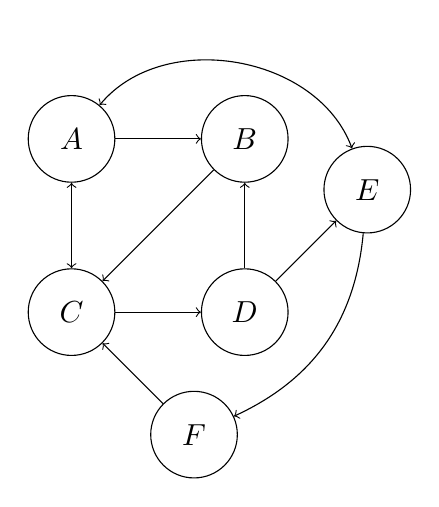
\begin{tikzpicture}[node distance={20mm},main/.style={draw, circle, scale=1.1, minimum size=10mm}]
            \node[main] (0) {$A$};          
            \node[main] (1) [right of=0] {$B$};
            \node[main] (2) [below of=0] {$C$};
            \node[main] (3) [below of=1] {$D$};
            \node[main] (4) [above right of=3] {$E$};
            \node[main] (5) [below right of=2] {$F$};
          
            \draw[->] (0) -- (1);
            \draw[<->] (0) -- (2);
            \draw[<-] (1) -- (3);
            \draw[->] (2) -- (3);
            \draw[<-] (2) -- (1);
            \draw[->] (3) -- (4);
            \draw[<-] (2) -- (5);
            \draw[<->] (0) edge[bend left=60] (4);
            \draw[<-] (5) edge[bend right] (4);
          \end{tikzpicture}
    }
    \hspace{1.5cm}
    \subfloat[\emph{Albero ordinato}]{
        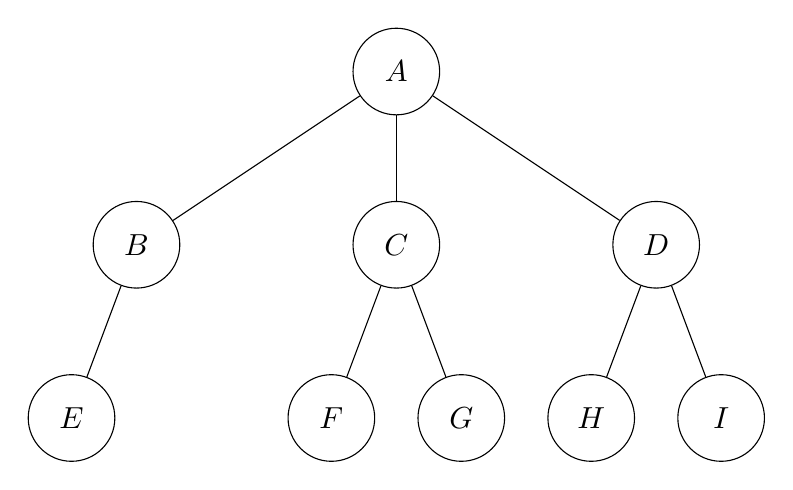
\begin{tikzpicture}[node distance={20mm},main/.style={draw, circle, scale=1.1, minimum size=10mm}]
            \node[main] (0) {$A$};
          
            \node[main] (2) [below of=0] {$C$};
            \node[main] (1) [left of=2, xshift=-10mm] {$B$};
            \node[main] (3) [right of=2, xshift=10mm] {$D$};
          
            \node[main] (4) [below of=1, xshift=-7.5mm] {$E$};
            \node[main] (5) [below of=2, xshift=-7.5mm] {$F$};
            \node[main] (6) [below of=2, xshift=7.5mm] {$G$};
            \node[main] (7) [below of=3, xshift=-7.5mm] {$H$};
            \node[main] (8) [below of=3, xshift=7.5mm] {$I$};
          
            \path[-]  (0) edge (1)
                      (0) edge (2)
                      (0) edge (3)
                      (1) edge (4)
                      (2) edge (5)
                      (2) edge (6)
                      (3) edge (7)
                      (3) edge (8);
          \end{tikzpicture}
    }
    \caption{\emph{Grafo} VS \emph{Albero ordinato}}
\end{figure}

\paragraph{Operazioni ammesse} Oltre a inserimento e rimozione, le operazioni
ammesse su \emph{grafi} e \emph{alberi} ruotano attorno alla possibilità di
accedere a tutti gli elementi delle strutture secondo diverse
\emph{visite}\footnote{Tutte le \emph{visite} saranno discusse nel dettaglio
nel prossimo capitolo}.

\subsection{Criticità nell'implementazione di strutture dati astratte}
Quando si implementa una \emph{struttura di dati astratta} può essere naturale
prediligere una particolare \emph{struttura di dati elementare} piuttosto che
un'altra. Ad esempio, viene naturale implementare una \emph{sequenza}
usando una \emph{lista}, o un \emph{albero astratto} come \emph{albero di
puntatori}. Tuttavia, esistono possibilità meno scontate, come l'utilizzo di
un vettore di booleani per l'implementazione di un \emph{insieme}, o un
\emph{albero} implementato come \emph{vettore dei padri}.

La \emph{struttura di dati elementare} scelta per l'implementazione di una
\emph{struttura dati astratta} si ripercuote sull'efficienza delle singole
operazioni. Per esempio, un \emph{dizionario} implementato come \emph{tabella
hash} permette di avere \emph{complessità} $O(1)$ nella funzione \texttt{lookup}
e $O(n)$ nella ricerca del minimo. Invece, lo stesso \emph{dizionario}
implementato come \emph{albero} porta la \emph{complessità} della \texttt{lookup}
a $O(\log n)$, ma riduce a $O(1)$ quella per la ricerca del minimo.

\newpage
\section{Strutture di dati elementari}
Vediamo ora le possibili implementazioni delle più comuni \emph{strutture
dati elementari}: \emph{liste}, \emph{pile} e \emph{code}.

\subsection{Liste}
\begin{definition}[Lista]
    Una lista è una sequenza di nodi contenenti dati arbitrati e uno o due
    puntatori all'elemento successivo e/o precedente.
\end{definition}
\begin{note}
    È importante notare che nodi contigui nella \emph{lista} non lo sono
    necessariamente anche in memoria.
\end{note}
\begin{note}
    In una \emph{lista} tutte le operazioni hanno costo $O(1)$.
\end{note}\noindent
Diverse implementazioni di una \emph{lista} possono essere categorizzate sulla
base di tre parametri:
\begin{itemize}
    \item \emph{Monodirezionali/Bidirezionali}: sono \emph{bidirezionali} le
    implementazioni in cui ogni nodo contiene due puntatori: uno all'elemento
    precedente, l'altro al successivo;
    \item \emph{Con sentinelle/Senza sentinella}: sono \emph{con sentinella}
    tutte le implementazioni in cui una \emph{lista} vuota ha un elemento;
    \item \emph{Circolare/Non circolare}: sono \emph{circolari} le
    implementazioni in cui l'ultimo elemento ha come successivo il primo, o
    viceversa;
\end{itemize}

\begin{figure}[ht]
    \centering
    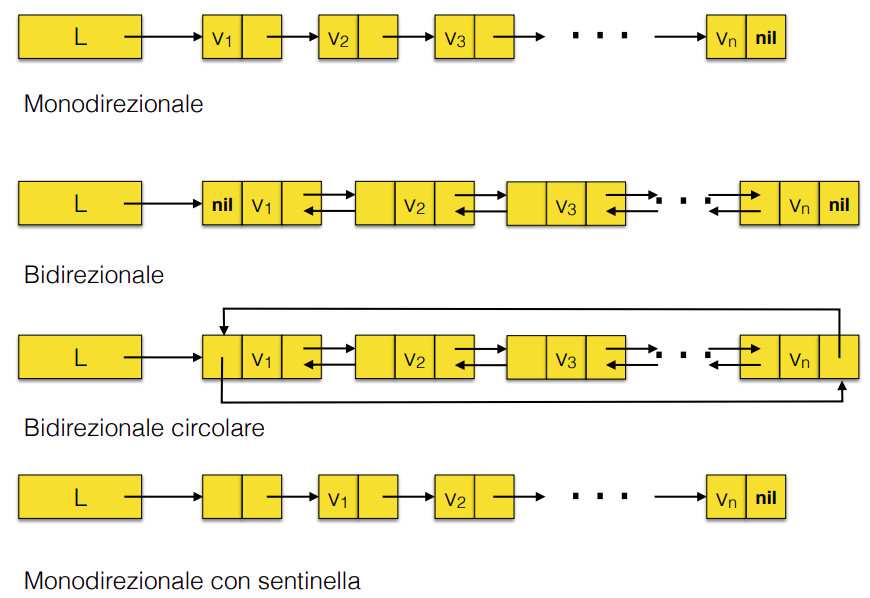
\includegraphics[width=0.9\textwidth]{tipi-liste.png}
    \caption{Diverse implementazioni di una \emph{lista}}
\end{figure}

\paragraph{Implementazione del tipo di dato POS}
\begin{code}{POS}
    \bc{POS} succ\hfill\com{Elemento successivo}
    \bc{POS} pred\hfill\com{Elemento precedente}
    \bc{ITEM} value\hfill\com{Valore}
    
    \ind\bc{POS} Pos(\bc{ITEM} v)\\
        \bc{POS} p = new \bc{POS}\\
        p.succ = nil\\
        p.pred = nil\\
        p.value = v
\end{code}

\paragraph{Implementazione di una lista bidirezionale con sentinella}
\begin{code}{Lista bidirezionale con sentinella}
    \begin{minipage}[t]{0.48\textwidth}
        \bc{LIST} pred\hfill\com{Predecessore}
        \bc{LIST} succ\hfill\com{Successore}
        \bc{ITEM} value\hfill\com{Valore}

        \ind\bc{LIST} List()\\
            \bc{LIST} t = new LIST\\
            t.pred = t\\
            t.succ = t\\
            return t\\

        \ind\bc{boolean} isEmpty()\\
            return (pred == succ == this)\\

        \ind\bc{POS} head()\\
            return succ\\

        \ind\bc{POS} tail()\\
            return pred\\

        \ind\bc{POS} next(\bc{POS} p)\\
            return p.succ\\

        \ind\bc{POS} prev(\bc{POS} p)\\
            return p.pred\\
    \end{minipage}
    \hfill
    \begin{minipage}[t]{0.48\textwidth}
        \par\noindent\com{Restituisce \bc{true} se $p$ è la}
        \com{posizione \emph{sentinella}}
        \rmbreak\ind\bc{boolean} finished(\bc{POS} p)\\
            return (p == this)\\

        \ind\bc{ITEM} read(\bc{POS} p)\\
            return p.value\\

        \ind write(\bc{POS} p, \bc{ITEM} v)\\
            p.value = v\\

        \ind\bc{POS} insert(\bc{POS} p, \bc{ITEM} v)\\
            \bc{POS} t = Pos(v)\\
            t.pred = p.pred\\
            p.pred.succ = t\\
            t.succ = p\\
            p.pred = t\\
            return t\\

        \ind\bc{POS} remove(\bc{POS} p)\\
            p.pred.succ = p.succ\\
            p.succ.pred = p.pred\\
            \bc{POS} t = p.succ\\
            delete p\\
            return t
        
    \end{minipage}
\end{code}
\begin{note}
    I tipi \texttt{POS} e \texttt{LIST} sono equivalenti.
\end{note}
\begin{note}
    Alla posizione \emph{sentinella} non è stato assegnato alcun valore
    in quanto serve soltanto a semplificare le operazioni di inserimento e
    rimozione.
\end{note}

\newpage
\subsection{Pile}
\begin{definition}[Pila]
    Una pila è una struttura dati dinamica e lineare, nella quale l'accesso agli
    elementi è definito in base all'ordine in cui sono stati inseriti. In
    particolare, è possibile accedere direttamente soltanto all'ultimo elemento
    inserito.
\end{definition}
\begin{note}
    Le \emph{pile} sono basate sull'approccio \emph{LIFO} (\emph{Last In, First
    Out}).
\end{note}

\paragraph{Specifica}
\begin{code}{Pila}
    \com{Restituisce \bc{true} se la \emph{pila} è vuota}
    \bc{boolean} isEmpty()
    \nl\com{Inserisce $v$ in cima alla pila}
    push(\bc{ITEM} v)
    \nl\com{Rimuove l'elemento in cima alla \emph{pila} e lo restituisce}
    \bc{ITEM} pop()
    \nl\com{Legge l'elemento in cima alla \emph{pila}}
    \bc{ITEM} top()
\end{code}
\begin{note}
    Nel gergo delle \emph{pile}, l'elemento \q{in cima} è l'ultimo elemento
    inserito, mentre quello \q{in fondo}, il primo.
\end{note}\noindent
Una \emph{pila} può essere implementata come \emph{vettore}, quindi di dimensione
limitata, o come \emph{lista bidirezionale} con puntatore all'elemento in testa.
\begin{figure}[h]
    \centering
    \subfloat[\emph{Pila} implementata come \emph{lista}]{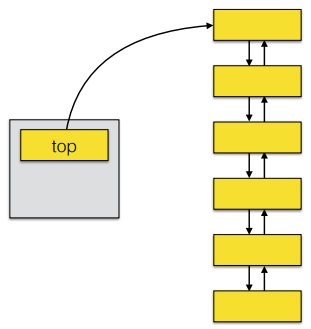
\includegraphics[width=0.4\textwidth, align=c]{pila-lista.png}}
    \hspace*{2cm}
    \subfloat[\emph{Pila} implementata come \emph{vettore}]{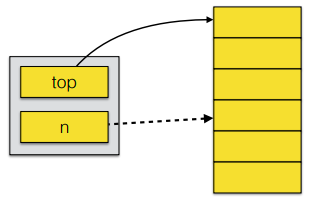
\includegraphics[width=0.4\textwidth, align=c]{pila-vettore.png}}
    \caption{Diverse implementazioni di una \emph{pila}}
\end{figure}

\newpage
\paragraph{Implementazione di una pila basata su vettore}
\begin{code}{Pila basata su vettore}
    \begin{minipage}[t]{0.48\textwidth}
        \bc{ITEM}[] V\hfill\com{Elementi}
        \bc{int} cur\hfill\com{Posizione cursore}
        \bc{int} max\_dim\hfill\com{Dimensione massima}

        \ind\bc{STACK} Stack(\bc{int} dim)\\
            \bc{STACK} t = new \bc{STACK}\\
            t.V = new \bc{int}[1\dots dim]\\
            t.V = new \bc{int}[1\dots dim]\\
            t.cur = 0\\
            t.max\_dim = dim\\
            return t\\
        
        \ind\bc{ITEM} top()\\
            precondition:(cur > 0)\\
            return V[cur]
    \end{minipage}
    \hfill
    \begin{minipage}[t]{0.48\textwidth}
        \ind\bc{boolean} isEmpty()\\
            return (cur == 0)\\

        \ind\bc{ITEM} pop()\\
            precondition:(cur > 0)\\
            \bc{ITEM} t = V[cur]\\
            cur = cur - 1\\
            return t\\

        \ind push(\bc{ITEM} v)\\
            precondition:(cur < max\_dim)\\
            cur = cur + 1\\
            V[cur] = v
    \end{minipage}
\end{code}
\begin{note}
    In una \emph{pila} implementata come \emph{lista} non è necessario specificare
    una dimensione massima.
\end{note}

\subsection{Code}
\begin{definition}[Coda]
    Una coda è una struttura dati dinamica e lineare, nella quale l'accesso agli
    elementi è definito in base all'ordine in cui sono stati inseriti. In
    particolare, è possibile accedere direttamente soltanto al primo elemento
    inserito.
\end{definition}
\begin{note}
    Le \emph{code} sono basate sull'approccio \emph{FIFO} (\emph{First In, First
    Out}).
\end{note}

\paragraph{Specifica}
\begin{code}{Coda}
    \com{Restituisce \bc{true} se la \emph{coda} è vuota}
    \bc{boolean} isEmpty()\\
    \com{Inserisce $v$ in fondo alla \emph{coda}}
    enqueue(\bc{ITEM} v)\\
    \com{Estrae l'elemento in testa alla \emph{coda} e lo restituisce al chiamante}
    \bc{ITEM} dequeue()\\
    \com{Legge l'elemento in testa alla \emph{coda}}
    \bc{ITEM} top()
\end{code}
\begin{note}
    Nel gergo delle \emph{code} l'elemento \q{in testa} è il primo inserito,
    mentre quello \q{in coda}, l'ultimo.
\end{note}\noindent
Una \emph{coda} può essere implementata come \emph{vettore circolare}, quindi di
dimensione limitata, o come \emph{lista monodirezionale} con puntatore
\emph{head} per l'estrazione e \emph{tail} per l'inserimento.

\paragraph{Implementazione di una coda basata su vettore circolare}
In un \emph{vettore circolare} gli indici possono essere gestiti efficientemente
facendo uso dell'operazione di \emph{modulo}. Bisogna tuttavia fare attenzione
alla gestione dei problemi di \emph{overflow}, provocati, non dall'accesso ad
aree di memoria esterne alla struttura (usando correttamente il \emph{modulo} ciò
è impossibile), ma dalla scrittura su valori non ancora letti. Questo
problema si propone quando il \emph{vettore} è pieno.

\bigskip\noindent Vediamo come questo problema può essere evitato.

Utilizzando due puntatori, \emph{read pointer} e \emph{write pointer}, che sono,
rispettivamente, il puntatore alla \emph{testa} e alla \emph{coda} della struttura,
si può fare in modo che non sia possibile scrivere nuovi valori quando il
\emph{write pointer} punta alla cella immediatamente precedente a quella puntata
dal \emph{read pointer}.

\bigskip\noindent Vediamo nel dettaglio graficamente:
\begin{figure}[h]
    \centering
    \subfloat[Prima scrittura]{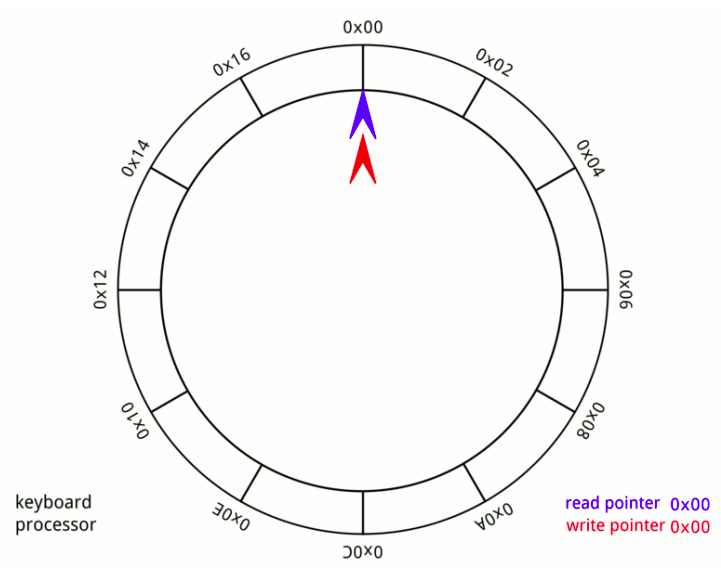
\includegraphics[align=c, width=0.50\textwidth]{coda-es-1.png}}
    \subfloat[Seconda scrittura]{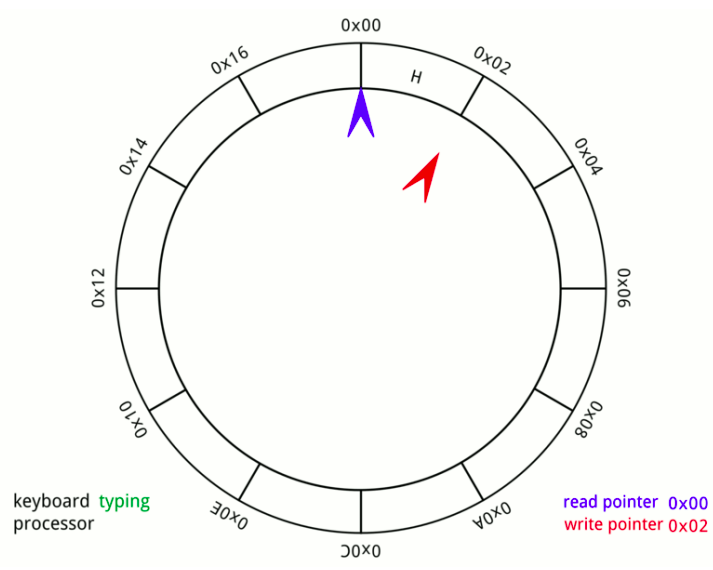
\includegraphics[align=c, width=0.50\textwidth]{coda-es-2.png}}\\
    \subfloat[Prima lettura]{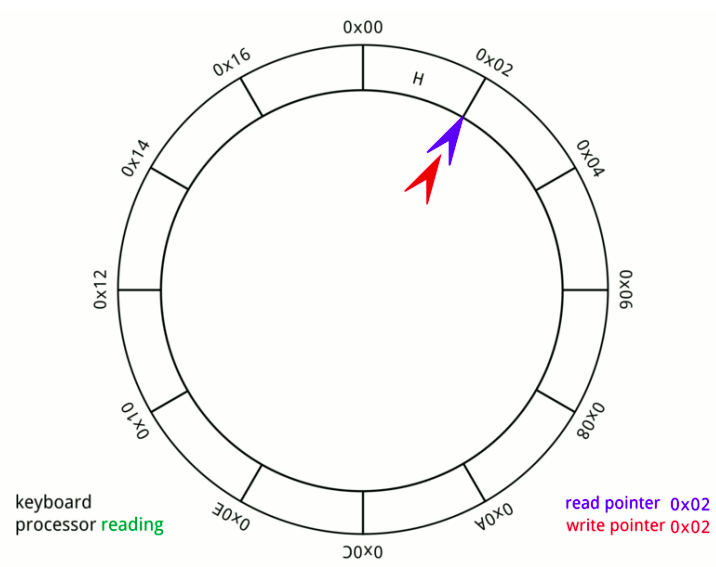
\includegraphics[align=c, width=0.50\textwidth]{coda-es-3.png}}
    \subfloat[Seconda lettura]{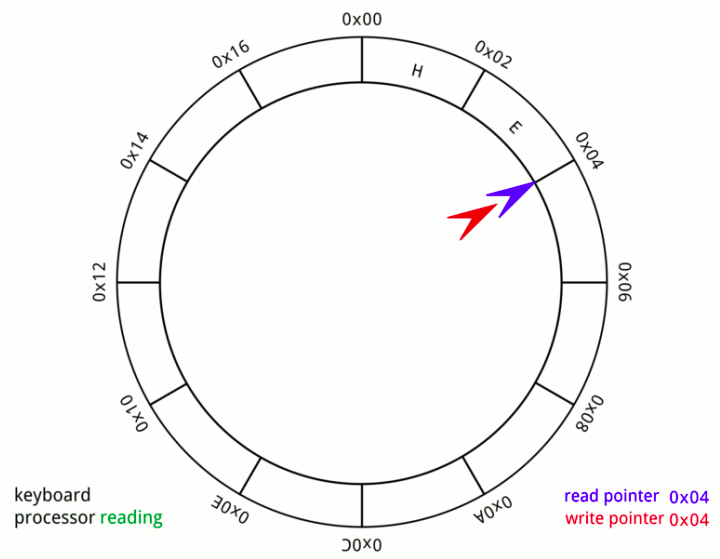
\includegraphics[align=c, width=0.50\textwidth]{coda-es-4.png}}\\
\end{figure}\newpage
\begin{figure}[ht]\ContinuedFloat
    \centering
    \subfloat[Ultima scrittura su cella libera]{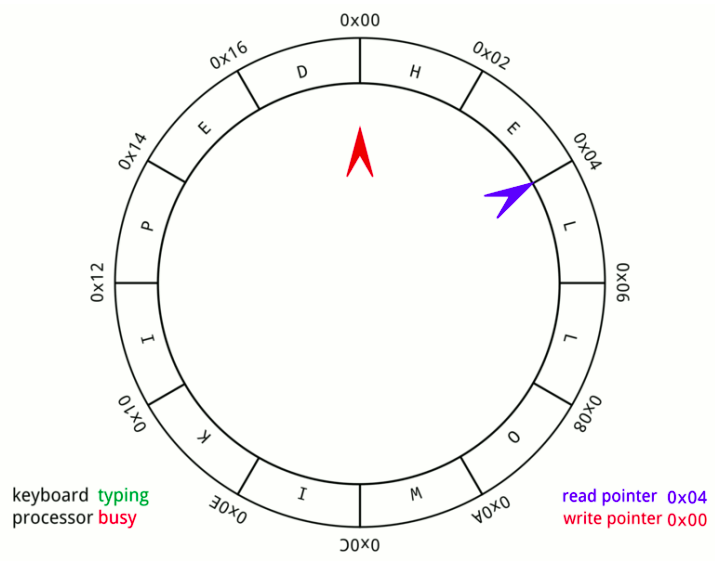
\includegraphics[align=c, width=0.50\textwidth]{coda-es-5.png}}
    \subfloat[Prima scrittura su cella già letta]{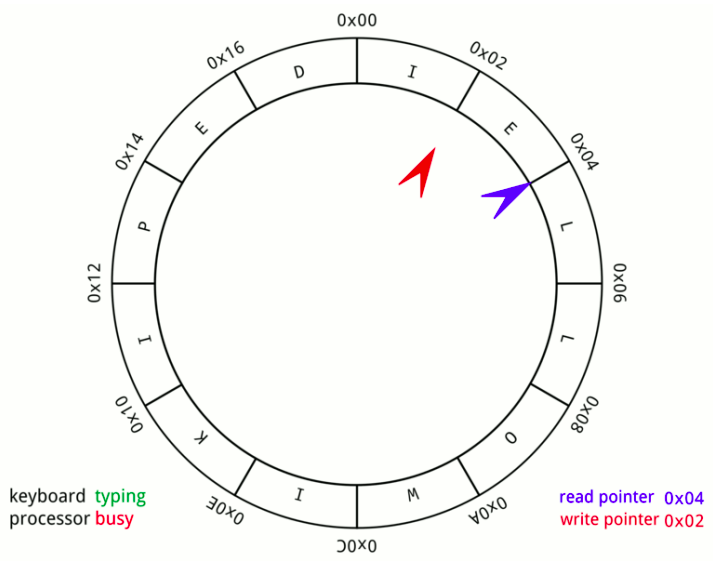
\includegraphics[align=c, width=0.50\textwidth]{coda-es-6.png}}\\
    \subfloat[Blocco delle scritture]{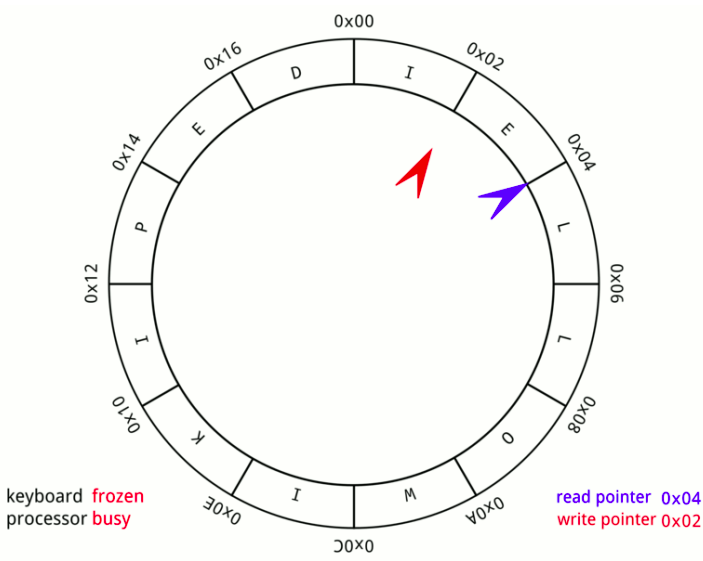
\includegraphics[align=c, width=0.50\textwidth]{coda-es-7.png}}
    \subfloat[Lettura di tutte le celle]{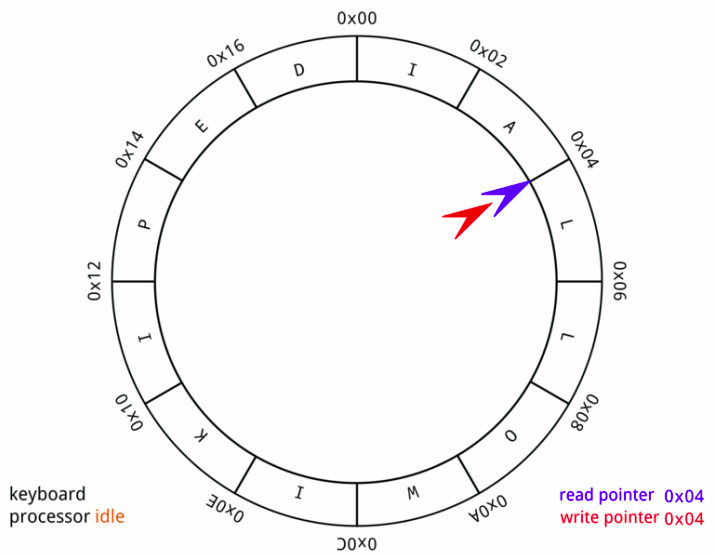
\includegraphics[align=c, width=0.50\textwidth]{coda-es-8.png}}
    \caption{Esempio di esecuzione di una \emph{coda} implementata come \emph{vettore circolare}}
\end{figure}\noindent
Nelle immagini di cui sopra si vede molto bene come, dopo ogni operazione di lettura
e scrittura, i rispettivi puntatori avanzino fino alla cella successiva.
Fino a quando ci sono celle libere i due puntatori avanzano in modo indipendente,
ma quando queste finiscono, le successive scritture vanno a sovrascrivere i
valori precedentemente inseriti e che sono stati già letti.

Una volta che il \emph{write pointer} si trova sulla cella che precede quella
indicata dal \emph{read pointer}, la \emph{coda} è piena e quindi non è possibile
inserire nuovi elementi fino a quando non ne vengono letti alcuni. Quando invece
il \emph{read pointer} va a sovrapporsi al \emph{write pointer} significa che la
\emph{coda} è stata svuotata e di conseguenza vengono bloccate le letture.

\newpage
\begin{code}{Coda basata su vettore circolare}
    \begin{minipage}[t]{0.48\textwidth}
        \bc{ITEM}[] V\hfill\com{Elementi}
        \bc{int} cur\_dim\hfill\com{Dimensione attuale}
        \bc{int} head\hfill\com{Testa della \emph{coda}}
        \bc{int} max\_dim\hfill\com{Dimensione massima}

        \ind\bc{QUEUE} Queue(\bc{int} dim)\\
            \bc{QUEUE} t = new \bc{QUEUE}\\
            t.V = new \bc{int}[dim]\\
            t.max\_dim = dim\\
            t.head = 0\\
            t.cur\_dim = 0\\
            return t\\

        \ind\bc{ITEM} top()\\
            precondition:(cur\_dim > 0)\\
            return V[head]\\
    \end{minipage}
    \hfill
    \begin{minipage}[t]{0.48\textwidth}
        \ind\bc{boolean} isEmpty()\\
            return (cur\_dim == 0)\\

        \ind\bc{ITEM} dequeue()\\
            precondition:(cur\_dim > 0)\\
            \bc{ITEM} t = V[head]\\
            head = (head + 1) mod max\_dim\\
            cur\_dim = cur\_dim - 1\\
            return t\\

        \ind enqueue(\bc{ITEM} v)\\
            precondition:(cur\_dim < max\_dim)\\
            V[(head + cur\_dim) mod max\_dim] = v\\
            cur\_dim = cur\_dim + 1
    \end{minipage}
\end{code}
\begin{note}
    In una \emph{coda} implementata come \emph{lista} non è necessario specificare
    una dimensione massima.
\end{note}
\chapter{Alberi binari e alberi generici}
\section{Introduzione}
Iniziamo con una definizione:
\begin{definition}[Albero radicato]
    Un albero radicato consiste di un insieme di nodi e di archi orientati che
    connettono coppie di nodi con le seguenti proprietà:
    \begin{itemize}
        \item Un nodo dell'albero è designato come nodo radice;
        \item Ogni nodo $n$, a parte la radice, ha esattamente un arco entrante;
        \item Per ogni nodo esiste un unico cammino che parte dalla radice e
        raggiunge quel nodo;
        \item L'albero è connesso;
    \end{itemize}
\end{definition}
\begin{definition}[Albero radicato (definizione ricorsiva)]
    Un albero radicato è definito come un insieme vuoto, oppure un nodo radice
    e zero o più sottoalberi, ognuno dei quali è un albero radice. La radice è
    connessa alla radice di ogni sottoalbero con un arco orientato.
\end{definition}

\subsection{Terminologia}
\begin{figure}[h!]
    \centering
    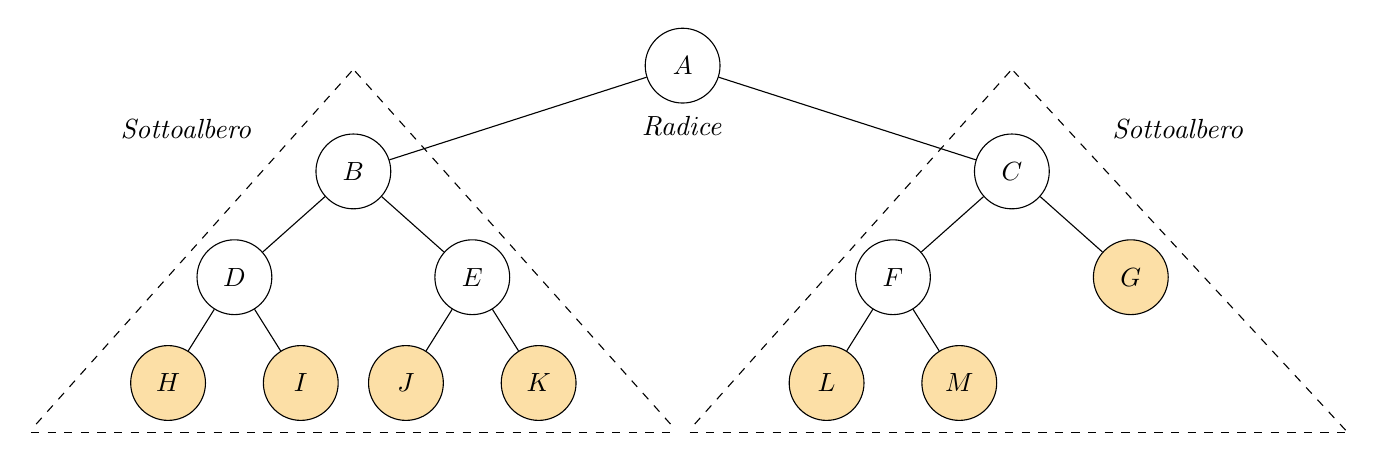
\begin{tikzpicture}[baseline={(0,0)},node distance={20mm},main/.style={draw, circle, scale=0.95, minimum size=10mm}]
        \node[main] (0) {$A$};
        
        \node[main] (1) [below left of=0, xshift=-85] {$B$};
        \node[main] (2) [below right of=0, xshift=85] {$C$};
      
        \node[main] (3) [below left of=1, xshift=-5] {$D$};
        \node[main] (4) [below right of=1, xshift=5] {$E$};
        \node[main] (5) [below left of=2, xshift=-5] {$F$};
        \node[main, fill=leaf] (6) [below right of=2, xshift=5] {$G$};
      
        \node[main, fill=leaf] (7) [below left of=3, xshift=15] {$H$};
        \node[main, fill=leaf] (8) [below right of=3, xshift=-15] {$I$};
        \node[main, fill=leaf] (9) [below left of=4, xshift=15] {$J$};
        \node[main, fill=leaf] (10) [below right of=4, xshift=-15] {$K$};
        \node[main, fill=leaf] (11) [below left of=5, xshift=15] {$L$};
        \node[main, fill=leaf] (12) [below right of=5, xshift=-15] {$M$};
      
        \path[-] (0) edge (1)
                 (0) edge (2)
                 (1) edge (3)
                 (1) edge (4)
                 (2) edge (5)
                 (2) edge (6)
                 (3) edge (7)
                 (3) edge (8)
                 (4) edge (9)
                 (4) edge (10)
                 (5) edge (11)
                 (5) edge (12);
      
        \node[] (13) [above of=1, yshift=-20, inner sep=0] {};
        \node[] (14) [below left of=7, yshift=22.5, xshift=-10, inner sep=0] {};
        \node[] (15) [below right of=10, yshift=22.5, xshift=10, inner sep=0] {};
      
        \path[-]  (13) edge[dashed] (14)
                  (13) edge[dashed] (15)
                  (14) edge[dashed] (15);
      
        \node[] (16) [above of=2, yshift=-20, inner sep=0] {};
        \node[] (17) [below left of=11, yshift=22.5, xshift=-10, inner sep=0] {};
        \node[] (18) [below right of=12, yshift=22.5, xshift=100, inner sep=0] {};
      
        \path[-]  (16) edge[dashed] (17)
                  (17) edge[dashed] (18)
                  (18) edge[dashed] (16);
        
        \node[] (19) [below of=0, yshift=35] {\emph{Radice}};
        \node[] (20) [above left of=1, yshift=-25, xshift=-20] {\emph{Sottoalbero}};
        \node[] (21) [above right of=2, yshift=-25, xshift=20] {\emph{Sottoalbero}};
      \end{tikzpicture}
\end{figure}\noindent
Partendo dallo schema di cui sopra possiamo definire la seguente terminologia:

\medskip\noindent\begin{minipage}[t]{0.48\textwidth}
    \begin{itemize}
        \item $A$ è la \emph{radice};
        \item $B$ e $C$ sono \emph{radici} dei \emph{sottoalberi};
        \item $D$ ed $E$ sono \emph{fratelli};
        \item $D$ ed $E$ sono \emph{figli} di $B$;
    \end{itemize}
\end{minipage}
\hfill
\begin{minipage}[t]{0.48\textwidth}
    \begin{itemize}
        \item $B$ è il \emph{padre} di $D$ ed $E$;
        \item I \emph{nodi} gialli sono \emph{foglie};
        \item Gli altri \emph{nodi} sono \emph{nodi interni};
    \end{itemize}
\end{minipage}

\bigskip\noindent
Per ogni \emph{albero} possiamo poi definire i seguenti parametri:
\begin{definition}[Profondità di un nodo (depth)]
    È definita profondità di un nodo la lunghezza del cammino semplice dalla
    radice al nodo. La lunghezza è misurata in numero di archi attraversati.
\end{definition}
\begin{definition}[Livello (level)]
    È definito livello l'insieme dei nodi alla stessa profondità
\end{definition}
\begin{definition}[Altezza di un albero (height)]
    È definita altezza di un albero la profondità massima della sue foglie.
\end{definition}

\begin{figure}[h]
\centering
\begin{tikzpicture}[node distance={20mm},main/.style={draw, circle, scale=0.95}]
    \node[] (0) {};
    \node[] (1) [left of=0, xshift=80mm] {\emph{Livello}};

    \node[main] (3) [below of=0, yshift=10mm] {$L_0$};
    \node[] (2) [left of=3, xshift=80mm] {$0$};

    \node[main] (5) [below left of=3, xshift=-30mm] {$L_1$};
    \node[main] (6) [below right of=3, xshift=30mm] {$L_1$};
    \node[] (4) [below of=2, yshift=6.5mm] {$1$};

    \node[main] (7) [below left of=5, xshift=-10mm] {$L_2$};
    \node[main] (8) [below right of=5, xshift=10mm] {$L_2$};
    \node[main] (9) [below left of=6, xshift=-10mm] {$L_2$};
    \node[] (14) [below of=4, yshift=6.75mm] {$2$};
    
    \node[main] (10) [below left of=7, xshift=5mm] {$L_3$};
    \node[main] (11) [below right of=7, xshift=-5mm] {$L_3$};
    \node[main] (12) [below left of=8, xshift=5mm] {$L_3$};
    \node[main] (13) [below right of=8, xshift=-5mm] {$L_3$};
    \node[] (15) [below of=14, yshift=6.75mm] {$3$};

    \draw (3) -- (5);
    \draw (3) -- (6);
    \draw (5) -- (7);
    \draw (5) -- (8);
    \draw (6) -- (9);
    \draw (7) -- (10);
    \draw (7) -- (11);
    \draw (8) -- (12);
    \draw (8) -- (13);
\end{tikzpicture}
\caption{\emph{Albero} di \emph{altezza} $3$}
\end{figure}

\section{Alberi binari}
\begin{definition}[Albero binario]
    Un albero binario è un albero radicato in cui ogni nodo ha al più due figli,
    identificati come figlio sinistro e figlio destro.
\end{definition}
\begin{note}
    Due \emph{alberi} $T$ e $U$ che hanno gli stessi \emph{nodi}, gli stessi
    \emph{figli} per ogni \emph{nodo} e la stessa \emph{radice}, sono distinti
    qualora un \emph{nodo} $u$ sia designato come \emph{figlio sinistro} di $v$
    in $T$ e come \emph{figlio destro} di $v$ in $U$.
\end{note}

\subsection{Specifica}
\begin{code}{Albero binario}
    \com{Costituisce un nuovo \emph{nodo}, contenente $v$, senza \emph{figli} o
    \emph{genitori}}
    Tree(\bc{ITEM}  v)
    \nl\com{Legge il valore memorizzato nel \emph{nodo}}
    \bc{ITEM} read()
    \nl\com{Modifica il valore memorizzato nel \emph{nodo}}
    write(\bc{ITEM} v)
    \nl\com{Restituisce il \emph{padre}, oppure nil se questo è il \emph{nodo
    radice}}
    \bc{TREE} parent()
    \nl\com{Restituisce il \emph{figlio sinistro} di questo \emph{nodo}, oppure
    nil se è assente}
    \bc{TREE} left()
    \nl\com{Restituisce il \emph{figlio destro} di questo \emph{nodo}, oppure
    nil se è assente}
    \bc{TREE} right()
    \nl\com{Inserisce il \emph{sottoalbero radicato} $t$ come \emph{figlio sinistro}
    di questo \emph{nodo}}
    insertLeft(\bc{TREE} t)
    \nl\com{Inserisce il \emph{sottoalbero radicato} $t$ come \emph{figlio destro}
    di questo \emph{nodo}}
    insertRight(\bc{TREE} t)
    \nl\com{Distrugge ricorsivamente il \emph{figlio sinistro} di questo \emph{nodo}}
    deleteLeft()
    \nl\com{Distrugge ricorsivamente il \emph{figlio destro} di questo \emph{nodo}}
    deleteRight()
\end{code}

\subsection{Memorizzazione di un albero binario}
In memoria, per ogni \emph{nodo}, memorizziamo un puntatore al \emph{nodo padre}
(\texttt{P}), che sarà \texttt{nil} nel caso della \emph{radice}, e altri due
puntatori, contenenti, rispettivamente, il riferimento al \emph{figlio sinistro}
(\texttt{L}) e \emph{destro} (\texttt{R}) di quel \emph{nodo}.
Nel caso di \emph{nodi foglia}, quei puntatori saranno entrambi \texttt{nil}.
\begin{figure}[h!]
    \centering
    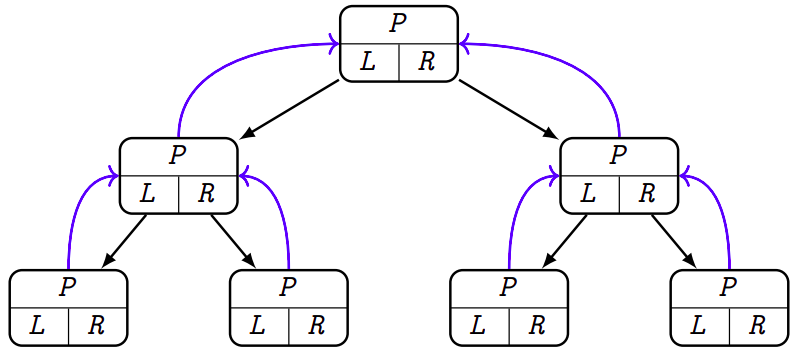
\includegraphics[width=0.7\textwidth]{memorizzazione-albero-binario.png}
    \caption{Schema di memorizzazione di un \emph{albero binario}}
\end{figure}

\subsection{Implementazione di un albero binario}
\begin{code}{Implementazione di un albero binario}
    \begin{minipage}[t]{0.48\textwidth}
        \ind Tree(\bc{ITEM} v)\\
            \bc{TREE} t = new \bc{TREE}\\
            t.parent = nil\\
            t.left = nil\\
            t.right = nil\\
            t.value = v\\
            return t\\
        
        \ind\bc{ITEM} read()\\
            return value\\

        \ind write(\bc{ITEM} v)\\
            value = v\\

        \ind\bc{TREE} parent()\\
            return parent\\

        \ind\bc{TREE} left()\\
            return left\\

        \ind\bc{TREE} right()\\
            return right\\
    \end{minipage}
    \hfill
    \begin{minipage}[t]{0.48\textwidth}
        \com{Ipotizziamo che sia possibile}
        \com{inserire un \emph{figlio} solo se non}
        \com{ne esiste già uno}
        \rmbreak\ind insertLeft(\bc{TREE} t)\\
            \indf if (left == nil) then\\
                t.parent = this\\
                left = t\\

        \ind insertRight(\bc{TREE} t)\\
            \indf if (right == nil) then\\
                t.parent = this\\
                right = t\\

        \ind deleteLeft()\\
            \indf if (left $\neq$ nil) then\\
                left.deleteLeft()\\
                left.deleteRight()\\
                delete left\\
                left = nil\\
            
        \ind deleteRight()\\
            \indf if (right $\neq$ nil) then\\
                right.deleteLeft()\\
                right.deleteRight()\\
                delete right\\
                right = nil\\
    \end{minipage}
\end{code}

\subsection{Visite di un albero binario}
\begin{definition}[Visita di un albero]
    Una visita è una strategia per visitare tutti i nodi dell'albero.
\end{definition}
\begin{definition}[Visita in profondità (depth first search)]
    Una visita in profondità è un tipo di visita nella quale vengono visitati
    ricorsivamente tutti i sottoalberi.
\end{definition}
\begin{note}
    Questo tipo di \emph{visita} richiede l'utilizzo di una \emph{pila}.
\end{note}\noindent
Per la \emph{visita in profondità} esistono tre varianti che si differenziano per
il momento in cui viene utilizzato il valore di un \emph{nodo}:
\begin{itemize}
    \item \emph{Visita in Pre-order}: il valore del \emph{nodo} viene usato prima
    di visitare i \emph{sottoalberi};
    \item \emph{Visita in In-order}: il valore del \emph{nodo} viene usato dopo
    aver visitato il \emph{sottoalbero di sinistra} e prima di visitare quello di
    \emph{destra};
    \item \emph{Visita in Post-order}: il valore del \emph{nodo} viene usato dopo
    aver visitato i \emph{sottoalberi}; 
\end{itemize}

\begin{definition}[Visita in ampiezza (breadth first search)]
    Una visita in ampiezza è un tipo di visita nella quale l'albero viene
    visitato un livello alla volta partendo dalla radice. 
\end{definition}
\begin{note}
    Questo tipo di \emph{visita} richiede l'utilizzo di una \emph{coda}.
\end{note}

\paragraph{Implementazione delle visite}
\begin{code}{Implementazione delle visite}
    \begin{minipage}[t]{0.48\textwidth}
        \com{Depth-First-Search in Pre-order}
        \rmbreak\ind dfs\_pre\_order(\bc{TREE} t)\\
            \indf if (t $\neq$ nil) then\\
                print t.value\\
                dfs\_pre\_order(t.left)\\
                dfs\_pre\_order(t.right)\\

        \noindent\com{Depth-First-Search in In-order}
        \rmbreak\ind dfs\_in\_order(\bc{TREE} t)\\
            \indf if (t $\neq$ nil) then\\
                dfs\_in\_order(t.left)\\
                print t.value\\
                dfs\_in\_order(t.right)\\

        \noindent\com{Depth-First-Search in Post-order}
        \rmbreak\ind dfs\_post\_order(\bc{TREE} t)\\
            \indf if (t $\neq$ nil) then\\
                dfs\_post\_order(t.left)\\
                dfs\_post\_order(t.right)\\
                print t.value\\
    \end{minipage}
    \hfill
    \begin{minipage}[t]{0.48\textwidth}
        \com{Breadth-First-Search}
        \rmbreak\ind bfs(\bc{TREE} t)\\
            \bc{QUEUE} q = Queue()\\
            q.enqueue(t)\\
            \indf while (not q.isEmpty()) do\\
                \bc{TREE} u = q.dequeue()\\
                print u.value\\
                \com{Accoda entrambi i \emph{figli}}
                \com{del \emph{nodo} corrente}
                u = u.left()\\
                \indff if (u $\neq$ nil) then\\
                    q.enqueue(u)\\
                
                \rmbreak\indf\\
                u = u.parent().right()\\
                \indff if (u $\neq$ nil) then\\
                    q.enqueue(u)\\
    \end{minipage}
\end{code}\noindent
\paragraph{Esempi di visite}\mbox{}\\
\begin{minipage}[t]{0.48\textwidth}
    Vediamo un esempio di utilizzo delle \emph{visite}:
    \begin{itemize}
        \item \emph{DFS Pre-order}: \texttt{A B C D E F G};
        \item \emph{DFS In-order}: \texttt{C B D A F E G};
        \item \emph{DFS Post-order}: \texttt{C D B F G E A};
        \item \emph{BFS}: \texttt{A B E C D F G};
    \end{itemize}
\end{minipage}
\hfill
\begin{minipage}[t]{0.48\textwidth}
    \begin{center}
        \begin{graph}
          \node[main] (0) {$A$};
          \node[main] (1) [below left of=0, xshift=-15] {$B$};
          \node[main] (2) [below right of=0, xshift=15] {$E$};
          \node[main] (3) [below left of=1, xshift=10] {$C$};
          \node[main] (4) [below right of=1, xshift=-10] {$D$};
          \node[main] (5) [below left of=2, xshift=10] {$F$};
          \node[main] (6) [below right of=2, xshift=-10] {$G$};
      
          \path[-]  (0) edge (1)
                    (0) edge (2)
                    (1) edge (3)
                    (1) edge (4)
                    (2) edge (5)
                    (2) edge (6);
        \end{graph}
      \end{center}
\end{minipage}

\begin{note}
    Il \emph{costo computazionale} di una \emph{visita} di un \emph{albero}
    contenente $n$ \emph{nodi} è $\Theta(n)$ poiché ogni \emph{nodo} viene
    visitato una sola volta.
\end{note}

\newpage
\section{Alberi generici}
Negli \emph{alberi generici}, ovviamente, non possiamo parlare di \emph{figlio
sinistro} e \emph{figlio destro}, ma possiamo comunque distinguere i \emph{figli}
di un \emph{nodo} in base alla loro posizione. Parleremo infatti, di
\emph{figlio più a sinistra}, o \emph{primo figlio}, e \emph{fratello destro},
o \emph{prossimo fratello}.

\subsection{Specifica}
\begin{code}{Albero generico}
    \com{Costituisce un nuovo \emph{nodo}, contenente $v$, senza \emph{figli} o
    \emph{genitori}}
    Tree(\bc{ITEM}  v)
    \nl\com{Legge il valore memorizzato nel \emph{nodo}}
    \bc{ITEM} read()
    \nl\com{Modifica il valore memorizzato nel \emph{nodo}}
    write(\bc{ITEM} v)
    \nl\com{Restituisce il \emph{padre}, oppure nil se questo è il \emph{nodo
    radice}}
    \bc{TREE} parent()
    \nl\com{Restituisce il primo \emph{figlio} da sinistra, oppure nil se
    questo \emph{nodo}}
    \com{è una \emph{foglia}}
    \bc{TREE} leftmostChild()
    \nl\com{Restituisce il primo \emph{fratello} sulla destra, oppure nil se
    è assente}
    \bc{TREE} rightSibling()
    \nl\com{Inserisce il \emph{sottoalbero} $t$ come primo \emph{figlio} di
    questo \emph{nodo}}
    insertChild(\bc{TREE} t)
    \nl\com{Inserisce il \emph{sottoalbero} $t$ come prossimo \emph{fratello} di
    questo \emph{nodo}}
    insertSibling(\bc{TREE} t)
    \nl\com{Distrugge l'\emph{albero radicato} identificato dal primo \emph{figlio}}
    deleteChild()
    \nl\com{Distrugge l'\emph{albero radicato} identificato dal prossimo \emph{fratello}}
    deleteSibling()
    \nl\com{Distrugge l'\emph{albero radicato} identificato dal \emph{nodo}}
    delete(\bc{TREE} t)
\end{code}

\subsection{Memorizzazione di un albero generico}
A differenza degli \emph{alberi binari}, per gli \emph{alberi generici} esistono
diversi modi per rappresentarli in memoria. I modi sono tre:
\begin{itemize}
    \item \emph{Vettore dei figli}: ogni \emph{nodo} contiene un riferimento al
    \emph{padre} e un vettore contenente i puntatori ai \emph{figli};
    \item \emph{Primo figlio, prossimo fratello}: ogni \emph{nodo} contiene un
    riferimento al \emph{padre} e un riferimento al prossimo \emph{fratello};
    \item \emph{Vettore dei padri}: l'\emph{albero} è rappresentato da un
    vettore di coppie nelle quali il primo valore è il valore associato al
    \emph{nodo} e il secondo è l'indice della posizione del \emph{padre} nel
    vettore;
\end{itemize}

\begin{note}
    L'approccio con \emph{vettore dei figli} può causare uno spreco di memoria
    se molte celle di quei vettori puntano a \texttt{nil}.
\end{note}
\paragraph{Tecniche di memorizzazione a confronto}\mbox{}\\
\begin{figure}[h!]
    \centering
    \subfloat[\emph{Vettore dei figli}]{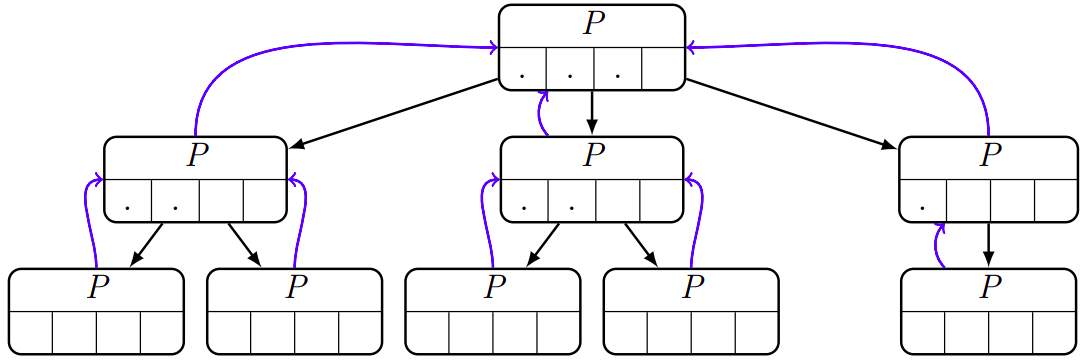
\includegraphics[width=0.48\textwidth]{vettore-dei-figli.png}}
    \hfill
    \subfloat[\emph{Primo figlio, prossimo fratello}]{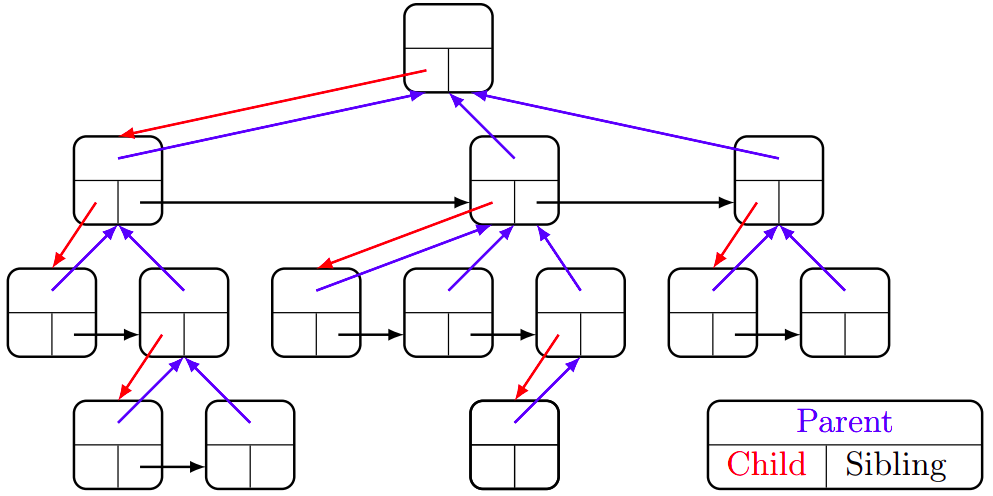
\includegraphics[width=0.48\textwidth]{vettore-dei-fratelli.png}}\\
    \subfloat[\emph{Vettore dei padri}]
    {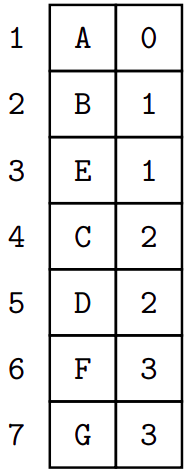
\includegraphics[width=0.1\textwidth, align=t]{vettore-dei-padri.png}
    \hspace{30pt}
    \begin{graph}
        \node[main] (0) [yshift=-15] {$A$};
        \node[main] (1) [below left of=0, xshift=-15] {$B$};
        \node[main] (2) [below right of=0, xshift=15] {$E$};
        \node[main] (3) [below left of=1, xshift=10] {$C$};
        \node[main] (4) [below right of=1, xshift=-10] {$D$};
        \node[main] (5) [below left of=2, xshift=10] {$F$};
        \node[main] (6) [below right of=2, xshift=-10] {$G$};
    
        \path[-]  (0) edge (1)
                  (0) edge (2)
                  (1) edge (3)
                  (1) edge (4)
                  (2) edge (5)
                  (2) edge (6);
    \end{graph}}
    \caption{Memorizzazione di \emph{alberi generici}}
\end{figure}

\subsection{Implementazione di un albero generico}
Di seguito, è riportata l'implementazione di un \emph{albero generico} realizzato
con la tecnica di memorizzazione \emph{primo figlio, prossimo fratello}.

\begin{code}{Implementazione di un albero generico}
    \begin{minipage}[t]{0.48\textwidth}
        \bc{TREE} parent\hfill\com{Riferimento al \emph{padre}}
        \bc{TREE} child\hfill\com{Riferimento al}
        \mbox{}\hfill\com{primo \emph{figlio}}
        \bc{TREE} sibling\hfill\com{Riferimento al}
        \mbox{}\hfill\com{prossimo \emph{fratello}}
        \bc{ITEM} value\hfill\com{Valore}

        \ind\bc{TREE} Tree(\bc{ITEM} v)\\
            \bc{TREE} t = new \bc{TREE}\\
            t.value = v\\
            t.parent = nil\\
            t.child = nil\\
            t.sibling = nil\\
            return t
    \end{minipage}
    \hfill
    \begin{minipage}[t]{0.48\textwidth}
        \vspace{-8.5pt}
        \com{Inserisce $t$ prima dell'attuale}
        \com{\emph{figlio}}
        \rmbreak\ind insertChild(\bc{TREE} t)\\
            t.parent = this\\
            t.sibling = child\\
            child = t\\
        
        \com{Inserisce $t$ prima dell'attuale}
        \com{prossimo \emph{fratello}}
        \rmbreak\ind insertSibling(\bc{TREE} t)\\
                t.parent = parent\\
                t.sibling = sibling\\
                sibling = t\\
    \end{minipage}
\end{code}
\begin{codecont}
    \begin{minipage}[t]{0.48\textwidth}
        \ind\bc{ITEM} read()\\
            return value\\

        \ind write(\bc{ITEM} v)\\
            value = v\\

        \ind\bc{TREE} parent()\\
            return parent\\
            
        \ind\bc{TREE} leftmostChild()\\
            return child\\

        \ind\bc{TREE} rightSibling()\\
            return sibling\\
    \end{minipage}
    \hfill
    \begin{minipage}[t]{0.48\textwidth}
        \ind deleteChild()\\
            \bc{TREE} c = child.rightSibling()\\
            delete(child)\\
            child = c\\

        \ind deleteSibling()\\
            \bc{TREE} s = sibling.rightSibling()\\
            delete(sibling)\\
            sibling = s\\

        \ind delete(\bc{TREE} t)\\
            \bc{TREE} u = t.leftmostChild()\\
            \indf while (u $\neq$ nil) do\\
                \bc{TREE} next = u.rightSibling()\\
                delete(u)\\
                u = next\\
            \indf delete t\\
    \end{minipage}
\end{codecont}

\subsection{Visite di un albero generico}
Anche per gli \emph{alberi generici} valgono le stesse \emph{visite} viste
per gli \emph{alberi binari} ad eccezione della \emph{visita In-order} perché
in questo caso non è ben definibile una situazione intermedia.

\paragraph{Implementazione delle visite}
\begin{code}{Implementazione delle visite}
    \begin{minipage}[t]{0.48\textwidth}
        \com{Depth-First-Search in Pre-order}
        \rmbreak\ind dfs\_pre\_order(\bc{TREE} t)\\
            \indf if (t $\neq$ nil) then\\
                print t.value\\
                \bc{TREE} u = t.leftmostChild()\\
                \indff while (u $\neq$ nil) do
                    dfs\_pre\_order(u)\\
                    u = u.rightSibling()\\

        \noindent\com{Depth-First-Search in Post-order}
        \rmbreak\ind dfs\_post\_order(\bc{TREE} t)\\
            \indf if (t $\neq$ nil) then\\
                \bc{TREE} u = t.leftmostChild()\\
                \indff while (u $\neq$ nil) do
                    dfs\_post\_order(u)\\
                    u = u.rightSibling()\\
                \indff print t.value\\
    \end{minipage}
    \hfill
    \begin{minipage}[t]{0.48\textwidth}
        \com{Breadth-First-Search}
        \rmbreak\ind bfs(\bc{TREE} t)\\
            \bc{QUEUE} q = Queue()\\
            q.enqueue(t)\\
            \indf while (not q.isEmpty()) do\\
                \bc{TREE} u = q.dequeue()\\
                print u.value\\
                \com{Accoda tutti i \emph{figli}}
                \com{del \emph{nodo} corrente}
                u = u.leftmostChild()\\
                \indff while (u $\neq$ nil) do\\
                    q.enqueue(u)\\
                    u = u.rightSibling()\\
    \end{minipage}
\end{code}
\chapter{Alberi binari di ricerca e alberi bilanciati}
\section{Alberi binari di ricerca}
Precedentemente abbiamo accennato al concetto di \hyperref[def:39]
{\emph{dizionario}}, ovvero una \emph{struttura dati} costituita da coppie
chiave-valore. Un \emph{dizionario} può essere implementato in molteplici modi e
come abbiamo visto, implementazioni diverse possono comportare \emph{complessità}
diverse per le singole operazioni che agiscono su quella \emph{struttura}.

Ad, esempio, la seguente tabella riporta le complessità delle operazioni per
tre possibili implementazioni:
\begin{table}[h]
    \renewcommand{\arraystretch}{1.2}
    \centering
    \begin{tabular}{|l|c|c|c|}
        \hline
        \textbf{Struttura dati} & \textbf{lookup} & \textbf{insert} & \textbf{remove}\\
        \hline
        Vettore ordinato & $O(\log n)$ & $O(1)$ & $O(n)$\\
        \hline
        Vettore non ordinato & $O(n)$ & $O(1)$ & $O(1)$\\
        \hline
        Lista non ordinata & $O(n)$ & $O(1)$ & $O(1)$\\
        \hline
    \end{tabular}
\end{table}

\begin{note}
    La \emph{complessità} delle operazioni di \texttt{insert} e \texttt{remove}
    per le implementazioni con \emph{vettore e lista non ordinati} è $O(1)$
    solo se si ipotizza che, nella \texttt{insert} non si debba verificare se
    l'elemento è già presente o meno, e nella \texttt{remove}, che si conosca
    già la posizione dell'elemento da rimuovere. Se non si fanno queste
    ipotesi, la \emph{complessità} diventa $O(n)$.
\end{note}\noindent
A questo punto ci chiediamo se non sia possibile implementare un \emph{dizionario}
sfruttando gli \emph{alberi binari}. Supponiamo che ogni \emph{nodo}
contenga una coppia formata da una chiave e un valore. E ipotizziamo anche che
le chiavi appartengano ad un insieme totalmente ordinato, cioè che sia sempre
possibile stabile se una chiave precede o meno un'altra.
L'implementazione di un \emph{nodo} dell'\emph{albero} potrebbe quindi essere:
\begin{code}{Nodo albero}
    \bc{TREE} parent\\
    \bc{TREE} left\\
    \bc{TREE} right\\
    \bc{ITEM} key, value
\end{code}\noindent
Poiché le chiavi sono ordinabili, possiamo ipotizzare che per ogni \emph{nodo}
$u$ valgano le seguenti due proprietà:
\begin{enumerate}
    \item Le chiavi contenute nel \emph{sottoalbero sinistro} di $u$ sono
    tutte minori di $u.key$;
    \item Le chiavi contenute nel \emph{sottoalbero destro} di $u$ sono
    tutte maggiori di $u.key$;
\end{enumerate}\newpage
\begin{note}
    Le proprietà appena definite permettono di realizzare un algoritmo di
    ricerca dicotomica.
\end{note}\noindent
Definiamo una regola generale:\
\begin{definition}[Albero binario di ricerca (ABR)]
    Un albero binario di ricerca è un albero binario nel quale per ogni nodo $u$
    vale:
    \begin{enumerate}
        \item Ogni nodo del sottoalbero sinistro ha un valore inferiore di quello
        del nodo $u$;
        \item Ogni nodo del sottoalbero destro ha un valore maggiore di quello
        del nodo $u$;
    \end{enumerate}
\end{definition}

\subsection{Specifica}
Per un \emph{dizionario} implementato come \emph{albero binario di ricerca}
possiamo definire la seguente \emph{specifica}.
\begin{code}{Dizionario come albero binario di ricerca}
    \com{Getter}
    \bc{TREE} parent()\\
    \bc{TREE} left()\\
    \bc{TREE} right()\\
    \bc{ITEM} key()\\
    \bc{ITEM} value()\\
    
    \noindent\com{Operazioni per il \emph{dizionario}}
    \bc{ITEM} lookup(\bc{ITEM} k)\\
    insert(\bc{ITEM} k, \bc{ITEM} v)\\
    remove(\bc{ITEM} k)\\
    
    \noindent\com{Operazioni definibili su un \emph{albero di ricerca binaria}}
    \nl\com{Restituisce il nodo successore di $t$, cioè il più piccolo}
    \com{tra i \emph{nodi} più grandi di $t$}
    \bc{TREE} successorNode(\bc{TREE} t)
    \nl\com{Restituisce il nodo predecessore di $t$, cioè il più grande}
    \com{tra i \emph{nodi} più piccoli di $t$}
    \bc{TREE} predecessorNode(\bc{TREE} t)
    \nl\com{Restituisce il \emph{nodo} con valore minore}
    \bc{TREE} min(\bc{TREE} t)
    \nl\com{Restituisce il \emph{nodo} con valore maggiore}
    \bc{TREE} max(\bc{TREE} t)\\

    \noindent\com{Funzioni interne ausiliarie}
    \nl\com{Restituisce il \emph{nodo} dell'\emph{albero} $t$ contenente la
    chiave $k$,}
    \com{se è presente, altrimenti nil}
    \bc{TREE} lookupNode(\bc{TREE} t, \bc{ITEM} k)
    \nl\com{Inserisce l'associazione chiave-valore $(k, v)$ nell'\emph{albero} $t$.}
    \com{Se la chiave è già presente sostituisce il valore associato, altrimenti}
    \com{viene inserita una nuova associazione.}
    \com{Se $t$ è nil restituisce il \emph{nodo} creato, altrimenti $t$}
    \bc{TREE} insertNode(\bc{TREE} t, \bc{ITEM} k, \bc{ITEM} v)
    \nl\com{Rimuove il \emph{nodo} associato alla chiave $k$ e restituisce la
    \emph{radice}}
    \com{dell'\emph{albero} (potrebbe essere stata cambiata)}
    \bc{TREE} removeNode(\bc{TREE} t, \bc{ITEM} k)
\end{code}

\paragraph{Implementazione dizionario}
Operazioni a parte, l'implementazione di \emph{dizionario} mediante \emph{albero
binario di ricerca} non è altro che:
\begin{code}{Dizionario come ABR}
    \bc{TREE} tree\\

    \ind Dictionary()\\
        tree = nil
\end{code}

\subsection{Ricerca}
L'implementazione della funzione \texttt{lookup} è banale:
\begin{minicode}{Dizionario come ABR - lookup}
    \ind\bc{ITEM} lookup(\bc{ITEM} k)\\
    \bc{TREE} t = lookupNode(tree, k)\\
    \indf if (t $\neq$ nil) then\\
        return t.value()\\
    \indf else\\
        return nil
\end{minicode}\noindent
La \texttt{lookupNode} può essere implementata sia in modo ricorsivo che
iterativo:
\begin{code}{Implementazione ricorsiva e iterativa di lookupNode}
    \begin{minipage}[t]{0.50\textwidth}
        \com{Versione ricorsiva}
        \rmbreak\ind\bc{TREE} lookupNode(\bc{TREE} t, \bc{ITEM} k)\\
            \indf if (t == nil or t.key == k) then\\
                return t\\
            \indf else\\
                \indff if (k < t.key) then\\
                    return lookupNode(t.left, k)\\
                \indff else\\
                    return lookupNode(t.right, k)\\
    \end{minipage}
    \hfill
    \begin{minipage}[t]{0.48\textwidth}
        \com{Versione iterativa}
        \rmbreak\ind\bc{TREE} lookupNode(\bc{TREE} t, \bc{ITEM} k)\\
            \bc{TREE} u = t\\
            \indf while (t $\neq$ nil and t.key $\neq$ k) do\\
                \indff if (k < u.key) then\\
                    \com{Sottoalbero di sinistra}
                    u = u.left\\
                \indff else\\
                    \com{Sottoalbero di destra}
                    u = u.right\\
            \indf return u
    \end{minipage}
\end{code}

\subsection{Massimo e minimo}
Grazie alle proprietà degli \emph{alberi binari di ricerca} la ricerca del
minimo e del massimo si riduce alla ricerca del \emph{nodo} più a sinistra
e più a destra dell'\emph{albero}.

\begin{code}{Implementazione minimo e massimo}
    \begin{minipage}[t]{0.48\textwidth}
        \com{Ricerca del minimo}
        \rmbreak\ind\bc{TREE} min(TREE t)\\
            \bc{TREE} u = t\\
            \indf if (u == nil) do\\
                return u\\
            \indf while (u.left $\neq$ nil) do\\
                u = u.left\\
            \indf return u
    \end{minipage}
    \hfill
    \begin{minipage}[t]{0.48\textwidth}
        \com{Ricerca del massimo}
        \rmbreak\ind\bc{TREE} max(TREE t)\\
            \bc{TREE} u = t\\
            \indf if (u == nil) do\\
                return u\\
            \indf while (u.right $\neq$ nil) do\\
                u = u.right\\
            \indf return u
    \end{minipage}
\end{code}

\subsection{Successore e predecessore}
\begin{definition}[Successore]
    Il successore di un nodo $u$ è il più piccolo nodo maggiore di $u$.
\end{definition}
\begin{definition}[Predecessore]
    Il predecessore di un nodo $u$ è il più grande nodo minore di $u$.
\end{definition}

\paragraph{Ricerca del successore}
Poiché il \emph{successore} di un \emph{nodo} è il più piccolo tra i \emph{nodi}
maggiori di esso, la ricerca del \emph{successore} di un \emph{nodo} $u$ non
può che essere fatta sui \emph{nodi} maggiori di $u$.
A questo punto quindi, si configurano due casi:
\begin{enumerate}
    \item \emph{$u$ ha un figlio destro}: il \emph{successore} di $u$ è
    il \emph{minimo} tra i \emph{nodi} del suo \emph{sottoalbero destro};
    \item \emph{$u$ non ha un figlio destro}: il \emph{successore}, se esiste, è
    uno degli \emph{avi} di $u$, ovvero uno dei \emph{nodi} superiori.
    Quindi, risalendo l'\emph{albero}, il \emph{successore} è il primo \emph{nodo}
    maggiore di $u$, cioè il primo \emph{nodo} per il quale $u$ sta nel suo
    \emph{sottoalbero sinistro};
\end{enumerate}

\begin{minicode}{Implementazione successore}
    \ind\bc{TREE} successorNode(\bc{TREE} t)\\
        \indf if (t == nil) then
            return t\\
        \indf if (t.right $\neq$ nil)\hfill\com{Caso 1:\,$t$ ha un \emph{figlio destro}}
            return min(t.right)\\
        \indf else\hfill\com{Caso 2:\,$t$ non ha un \emph{figlio destro}}
            \bc{TREE} p = t.parent\\
            \indff while (p $\neq$ nil and t == p.right) do\\
                t = p\\
                p = p.parent\\
            \indff return p
\end{minicode}

\paragraph{Ricerca del predecessore}
Per il \emph{predecessore} valgono le stesse considerazioni fatte per la
ricerca del \emph{successore}, ad eccezione del fatto che, se esiste, il
\emph{predecessore} di un \emph{nodo} $u$ sarà il massimo del suo \emph{sottoalbero
sinistro} oppure il primo \emph{avo} che ha $u$ come elemento del
\emph{sottoalbero destro}.

\begin{minicode}{Implementazione predecessore}
    \ind\bc{TREE} successorNode(\bc{TREE} t)\\
        \indf if (t == nil) then
            return t\\
        \indf if (t.left $\neq$ nil)\hfill\com{Caso 1:\,$t$ ha un \emph{figlio sinistro}}
            return max(t.left)\\
        \indf else\hfill\com{Caso 2:\,$t$ non ha un \emph{figlio sinistro}}
            \bc{TREE} p = t.parent\\
            \indff while (p $\neq$ nil and t == p.left) do\\
                t = p\\
                p = p.parent\\
            \indff return p
\end{minicode}

\subsection{Inserimento}
Per eseguire l'inserimento di una nuova associazione nel \emph{dizionario} è
sufficiente fare uso della funzione \texttt{insertNode}, che va ad inserire un
\emph{nodo}, o a modificarne uno esistente, in un \emph{albero binario di
ricerca}.
\begin{minicode}{Dizionario come ABR - insert}
    \ind insert(\bc{ITEM} k, \bc{ITEM} v)\\
        \indf tree = insertNode(tree, k, v)\\
\end{minicode}\noindent
Nemmeno l'implementazione della \texttt{insertNode} crea molti problemi, in quanto
è sufficiente applicare ricorsivamente le \hyperref[def:44]{\emph{proprietà degli
alberi binari di ricerca}}. Andremo quindi ad invocare ricorsivamente
l'\texttt{insertNode}, sul \emph{sottoalbero sinistro} o \emph{destro} a seconda
della relazione d'ordine tra il valore del nodo (i.e il valore della chiave
associata al \emph{nodo}) e il valore della chiave da inserire, fino al
raggiungimento di una \emph{foglia}, alla quale aggiungeremo un nuovo \emph{figlio
destro} o \emph{sinistro}, o di un \emph{nodo}, associato ad una chiave con lo
stesso valore di quella da inserire, nel qual caso sostituiremo il valore
salvato nel \emph{nodo} con quello nuovo.

Prima però di passare all'implementazione vera e propria, definiamo una
funzione ausiliaria \texttt{link} che presi due \emph{nodi} $p$, $u$ e una
chiave $k$, inserisce il \emph{nodo} $u$ come \emph{figlio sinistro} di $p$ se
$p.key > k$, altrimenti lo inserisce come \emph{figlio destro}.

\begin{minicode}{Implementazione link}
    \ind link(\bc{TREE} p, \bc{TREE} u, \bc{ITEM} k)\\
        \indf if (u $\neq$ nil) then\\
            u.parent = p\hfill\com{Inserisce il riferimento al \emph{padre}}
        \indf if (p $\neq$ nil) then\\
            \indff if (p.key > k) then\\
                p.left = u\hfill\com{Inserisce $u$ come \emph{figlio sinistro}}
            \indff else\\
                p.right = u\hfill\com{Inserisce $u$ come \emph{figlio destro}}
\end{minicode}

\begin{minicode}{Implementazione ricorsiva insertNode}
   \ind\bc{TREE} insertNode(\bc{TREE} t, \bc{ITEM} k, \bc{ITEM} v)\\
        \com{L'\emph{albero} è vuoto, quindi creo un nuovo \emph{nodo} e lo restituisco}
        \indf if (t == nil) then\\
            return Tree(k, v)\\
        \indf if (t.key == k) then\\
            t.value = v\hfill\com{L'associazione esiste già, per cui aggiorno il valore}
            return t\\
        \indf if (t.key > k) then\\
            \indff if (t.left == nil) then\hfill\com{Inserisce il \emph{nodo} come \emph{figlio sinistro}}
                link(t, Tree(k, v), k)\\
                return t\\
            \indff else\\
                return insertNode(t.left, k, v)\hfill\com{Continua a discendere l'\emph{albero}}
        \indf else\\
            \indff if (t.right == nil) then\hfill\com{Inserisce il \emph{nodo} come \emph{figlio destro}}
                link(t, Tree(k, v), k)\\
                return t\\
            \indff else\\
                return insertNode(t.right, k, v)\hfill\com{Continua a discendere l'\emph{albero}}
\end{minicode}\noindent
È anche possibile realizzare una versione iterativa della \texttt{insertNode}

\begin{minicode}{Implementazione iterativa insertNode}
\ind\bc{TREE} insertNode(\bc{TREE} t, \bc{ITEM} k, \bc{ITEM} v)\hfill\com{Riferimento al \emph{padre}}
    \bc{TREE} p = nil\\
    \bc{TREE} u = t\\
    \indf while (u $\neq$ nil and u.key $\neq$ k) do\hfill\com{Cerca la posizione di inserimento}
        p = u\\
        u = iif(k < u.key, u.left, u.right)\\
    \indf if (u $\neq$ nil and u.key == k) then\hfill\com{La chiave è già presente}
        u.value = v\\
    \indf else\\
        \bc{TREE} newTree = Tree(k, v)\hfill\com{Crea un nuovo \emph{nodo}}
        link(p, newTree, k)\hfill\com{Inserisce il nuovo \emph{nodo}}
        \indff if (p == nil) then\hfill\com{Il \emph{nodo creato è il primo dell'\emph{albero}}}
            t = newTree\\
    \indf return t\hfill\com{Restituisce il nuovo \emph{albero} o quello modificato}
\end{minicode}

\subsection{Cancellazione}
Come per la ricerca e l'inserimento, anche l'implementazione della funzione
\texttt{remove} è basata su un'altra funzione, la \texttt{removeNode}.

\begin{minicode}{Dizionario come ABR - remove}
    \ind remove(\bc{ITEM} k)\\
        tree = removeNode(tree, k)
\end{minicode}\noindent
L'implementazione della \texttt{removeNode} non è per nulla banale, in quanto, se
$u$ è il \emph{nodo} da eliminare, vanno considerate diverse casistiche:
\begin{enumerate}
    \item \emph{$u$ non ha figli}: si elimina il \emph{nodo};
    \item \emph{$u$ ha un figlio $f$}: si elimina $u$ e si rende $f$ il \emph{figlio}
    dell'\emph{ex-padre} di $u$ in sostituzione di $u$ (\emph{short-cut});
    \item \emph{$u$ ha due figli}: si individua il \emph{successore} $s$ di $u$.
    Poiché il \emph{successore}, per definizione, non ha \emph{figlio sinistro},
    si stacca $s$ dal proprio \emph{padre} e si attacca il suo \emph{figlio
    destro}, se esiste, come \emph{figlio sinistro} del \emph{padre} di $s$.
    Infine, si copia il valore di $s$ su $u$ e si elimina $s$;
\end{enumerate}

\begin{minicode}{Implementazione removeNode}
\ind\bc{TREE} removeNode(\bc{TREE} t, \bc{ITEM} k)\\
    \bc{TREE} u = lookupNode(t, k)\\
    \indf if (u $\neq$ nil) then\\
        \indff if (u.left == nil and u.right == nil) then\hfill\com{Caso 1}
            link(u.parent, nil, k)\hfill\com{Rimuove il \emph{figlio}}
            delete u\\
        \indff else if (u.left $\neq$ nil and u.right $\neq$ nil) then\hfill\com{Caso 3}
            \bc{TREE} s = successorNode(u)\\
            link(s.parent, s.right, s.key)\hfill\com{Attacca il \emph{figlio} di $s$ al \emph{padre} di $s$}
            u.key = s.key\hfill\com{Copia su $u$ la chiave di $s$}
            u.value = s.value\hfill\com{Copia su $u$ il valore di $s$}
            delete s\\
        \indff else if (u.left $\neq$ nil and u.right == nil)\hfill\com{Caso 2 con \emph{figlio sinistro}}
            link(u.parent, u.left, k)\\
            \indfff if (u.parent == nil) then\\
                t = u.left\\
        \indff else\hfill\com{Caso 2 con \emph{figlio destro}}
            link(u.parent, u.right, k)\\
            \indfff if (u.parent == nil) then\\
                t = u.right\\
    \indf return t
\end{minicode}\noindent
Vediamo la dimostrazione della correttezza di questa implementazione:
\begin{proof}[Dimostrazione]
    Procediamo caso per caso. Sia $u$ il \emph{nodo} che si
    intende rimuovere dall'\emph{albero}:
    \begin{enumerate}
        \item \emph{Nessun figlio}: eliminare \emph{foglie} non inficia
        sull'ordine degli altri nodi;
        \item \emph{Un solo figlio}:
        \begin{enumerate}
            \item \emph{Figlio destro}: se $u$ è il \emph{figlio destro} di $p$
            tutti i valori nell'\emph{albero} che ha come \emph{radice} $u$ sono
            maggiori di $p$;
            \item \emph{Figlio sinistro}: se $u$ è il \emph{figlio sinistro} di $p$
            tutti i valori nell'\emph{albero} che ha come \emph{radice} $u$ sono
            minori di $p$;
        \end{enumerate}
        \item \emph{Due figli}: il \emph{successore} $s$ del \emph{nodo} è
        maggiore di tutti i nodi del \emph{sottoalbero di sinistra} di $u$,
        ma allo stesso tempo, è anche minore di tutti i \emph{nodi} nel
        \emph{sottoalbero destro} di $u$, di conseguenza può essere sostituito
        a $u$;
    \end{enumerate}
\end{proof}

\subsection{Costo computazionale delle operazioni}
Tutte le operazioni viste per gli \emph{alberi binari di ricerca} sono
confinate ai \emph{nodi} posizionati lungo un cammino semplice dalla
\emph{radice} a una \emph{foglia}. Di conseguenza, se $h$ è l'\emph{altezza}
di un \emph{albero}, tutte le operazioni sono $O(h)$.

A questo punto vale la pena chiedersi quali siano il caso peggiore e quello
migliore.

\begin{figure}[h!]
    \centering
    \subfloat[Caso peggiore $h=O(n)$]
    {
        \begin{graph}
            \node[main, scale=0.8] (0) {$4$};
            \node[main, scale=0.8] (1) [below right of=0, xshift=-15] {$6$};
            \node[main, scale=0.8] (2) [below right of=1, xshift=-15] {$8$};
            \node[main, scale=0.8] (3) [below right of=2, xshift=-15] {$10$};
            \node[main, scale=0.8] (4) [below right of=3, xshift=-15] {$12$};
            \node[main, scale=0.8] (5) [below right of=4, xshift=-15] {$15$};
            \node[main, scale=0.8] (6) [below right of=5, xshift=-15] {$18$};
        
            \path[-]    (0) edge (1)
                        (1) edge (2)
                        (2) edge (3)
                        (3) edge (4)
                        (4) edge (5)
                        (5) edge (6);
        \end{graph}
    }
    \hspace{3cm}
    \subfloat[Caso migliore $h=O(\log n)$]
    {
        \begin{graph}
            \node[main] (0) [yshift=-107.5] {$10$};
            \node[main] (1) [below left of=0, xshift=-15] {$6$};
            \node[main] (2) [below right of=0, xshift=15] {$15$};
            \node[main] (3) [below left of=1, xshift=10] {$4$};
            \node[main] (4) [below right of=1, xshift=-10] {$8$};
            \node[main] (5) [below left of=2, xshift=10] {$12$};
            \node[main] (6) [below right of=2, xshift=-10] {$18$};
        
            \path[-]    (0) edge (1)
                        (0) edge (2)
                        (1) edge (3)
                        (1) edge (4)
                        (2) edge (5)
                        (2) edge (6);
        \end{graph}
    }
    \caption{\emph{Caso peggiore} e \emph{caso migliore}}
\end{figure}\noindent
Da queste immagini risulta evidente che sia meglio evitare di lavorare con \emph{alberi}
troppo \q{\emph{sbilanciati}}.

\section{Alberi binari di ricerca bilanciati}
Abbiamo terminato l'ultima sezione discutendo brevemente il modo in cui
l'\emph{altezza} di un \emph{albero} determini il costo delle operazioni. In
particolare, abbiamo accennato al fatto che nel caso pessimo tutti i \emph{nodi}
sono posizionati come in una \emph{lista}, mentre nel caso migliore
l'\emph{albero} gode una struttura più simmetrica rispetto alla \emph{radice}.

Ovviamente, nella maggior parte delle situazioni non si avrà a che fare né con
l'uno che con l'altro ed è quindi ragionevole attendersi, generalmente,
un'altezza inferiore a quella del caso pessimo. Addirittura, è dimostrato che
se gli elementi vengono inseriti in ordine casuale, l'\emph{altezza media} è
$O(\log n)$.

Nella realtà però, difficilmente ci si affida alla casualità e quindi, per
lavorare con \emph{alberi} di \emph{altezza} ottimale, si deve ricorrere a
tecniche che garantiscano un buon livello di \emph{bilanciamento}.

\begin{definition}[Fattore di bilanciamento]
    È definito fattore di bilanciamento di un nodo $v$ la massima differenza
    di l'altezza tra i suoi sottoalberi ed è indicato in simboli come $\beta(v)$.
\end{definition}\noindent
Esistono diversi algoritmi di \emph{bilanciamento}, quali ad esempio:
\begin{itemize}
    \item \emph{Alberi AVL} (Adelson-Veskii e Landis): bilanciano l'\emph{albero}
    facendo uso di rotazioni e garantiscono che per ogni \emph{nodo} $v$
    $\beta(v)\leq1$;
    \item \emph{B-alberi} (Bayer e McCreight): ogni \emph{nodo} $v$ ha
    $\beta(v)=0$ e sono specializzati per \emph{strutture} salvate in memoria
    secondaria;
    \item \emph{Alberi 2-3} (Hopcroft): ogni \emph{nodo} $v$ ha $\beta(v)=0$ e
    sono basati su una \emph{struttura} dinamica che attraverso operazioni di
    merge e split, distribuisce i \emph{nodi} su \emph{alberi} con due o tre
    \emph{figli};
\end{itemize}
In questa trattazione analizzeremo un quarto tipo di \emph{alberi}, gli
\emph{Alberi Red-Black}, ideati da Guibas e Sedgewick nel 1978.

\section{Alberi Red-Black}
\begin{definition}[Alberi Red-Black]
    Gli Alberi Red-Black sono alberi binari di ricerca nei quali ogni nodo è
    colorato di rosso oppure di nero. Le chiavi vengono mantenute soltanto nei
    nodi interni e le foglie sono costituite da nodi speciali con valore Nil.
    Inoltre, vengono rispettati i seguenti vincoli:
    \begin{enumerate}
        \item La radice è nera;
        \item Tutte le foglie sono nere;
        \item Entrambi i figli di un nodo rosso sono neri;
        \item Ogni cammino semplice da un nodo ad una delle sue foglie ha sempre
        lo stesso numero di nodi neri;
    \end{enumerate}
\end{definition}

\begin{figure}[h!]
    \centering
    \resizebox*{\textwidth}{!}{
        \begin{graph}
            \tikzset{rb/.style={main, font=\large\boldmath}}
            \tikzset{b/.style={rb, fill=black, color=black, text=red}}
            \tikzset{r/.style={rb, fill=red, color=red, text=black}}
            \tikzset{nil/.style={rectangle, fill=black, color=black, text=red, font=\ttfamily\large}}
        
            \node[b] (0) {$30$};
            \node[b] (1) [below left of=0, xshift=-100] {$15$};
            \node[b] (2) [below right of=0, xshift=100] {$70$};
        
            \node[b] (3) [below left of=1, xshift=-30] {$10$};
            \node[b] (4) [below right of=1, xshift=30] {$20$};
            \node[r] (5) [below left of=2, xshift=-30] {$60$};
            \node[b] (6) [below right of=2, xshift=30] {$85$};
        
            \node[r] (7) [below left of=3, xshift=7] {$5$};
            \node[b] (8) [below left of=5, xshift=7] {$50$};
            \node[b] (9) [below right of=5, xshift=-7] {$65$};
            \node[r] (10) [below left of=6, xshift=7] {$80$};
            \node[r] (11) [below right of=6, xshift=-7] {$90$};
        
            \node[r] (12) [below left of=8, xshift=24] {$40$};
            \node[r] (13) [below right of=8, xshift=-24] {$55$};
        
            \node[nil] (14) [below right of=3, xshift=-7] {Nil};
            \node[nil] (15) [below left of=4, xshift=7] {Nil};
            \node[nil] (16) [below right of=4, xshift=-7] {Nil};
        
            \node[nil] (23) [below left of=9, xshift=25, yshift=-5] {Nil};
            \node[nil] (24) [below right of=9, xshift=-25, yshift=-5] {Nil};
            \node[nil] (25) [below left of=10, xshift=25, yshift=-5] {Nil};
            \node[nil] (26) [below right of=10, xshift=-25, yshift=-5] {Nil};
            \node[nil] (27) [below left of=11, xshift=25, yshift=-5] {Nil};
            \node[nil] (28) [below right of=11, xshift=-25, yshift=-5] {Nil};
            \node[nil] (29) [below left of=7, xshift=25, yshift=-5] {Nil};
            \node[nil] (30) [below right of=7, xshift=-25, yshift=-5] {Nil};
        
            \node[nil] (31) [below left of=12, xshift=0] {Nil};
            \node[nil] (32) [below of=12, xshift=-3, yshift=16.5] {Nil};
            \node[nil] (33) [below of=13, xshift=3, yshift=16.5] {Nil};
            \node[nil] (34) [below right of=13, xshift=0] {Nil};
        
            \path[-]  (0) edge (1)
                      (0) edge (2)
                      (1) edge (3)
                      (1) edge (4)
                      (2) edge (5)
                      (2) edge (6)
                      (3) edge (7)
                      (5) edge (8)
                      (5) edge (9)
                      (6) edge (10)
                      (6) edge (11)
                      (8) edge (12)
                      (8) edge (13);
        
            \path[-]  (3) edge (14)
                      (4) edge (15)
                      (4) edge (16)
                      (9) edge (23)
                      (9) edge (24)
                      (10) edge (25)
                      (10) edge (26)
                      (11) edge (27)
                      (11) edge (28)
                      (7) edge (29)
                      (7) edge (30)
                      (12) edge (31)
                      (12) edge (32)
                      (13) edge (33)
                      (13) edge (34);
        \end{graph}
    }
    \caption{\emph{Albero Red-Black}}
    \label{fig:albero-red-black}
\end{figure}\noindent
Diamo inoltre le seguenti definizioni:
\begin{definition}[Altezza nera di un nodo]
    Dato un nodo $v$, l'altezza nera di quel nodo, indicata come $bh(v)$, è il
    numero di nodi neri lungo ogni cammino da $v$ (escluso) ad ogni sua foglia
    (inclusa).
\end{definition}
\begin{definition}[Altezza nera di un Albero Red-Black]
    L'altezza nera di un Albero Red-Black corrisponde all'altezza nera della
    sua radice.
\end{definition}\noindent
L'\emph{albero} della figura \ref{fig:albero-red-black} ha \emph{altezza nera}
pari a 3.

\begin{note}
    Per ogni \emph{Albero Red-Black} sono possibili più colorazioni che
    possono anche portare ad \emph{altezze nere} diverse.
\end{note}

\paragraph{Foglie come nodi Nil}
Come detto, le \emph{foglie} sono rappresentate da speciali \emph{nodi} con
valore \texttt{Nil}. Questo significa, che invece di un puntatore \texttt{nil},
c'è un riferimento ad un \emph{nodo} \texttt{Nil} di colore nero. E, poiché
tutti i \emph{nodi} \texttt{Nil} sono uguali, ne esiste uno solo al quale fanno
riferimento tutti i \emph{nodi} che hanno delle \emph{foglie}.

In realtà, i \emph{nodi} che hanno come \emph{figli} questo tipo di \emph{nodi},
sono essi stessi le vere foglie dell'\emph{albero}, in quanto, i \emph{nodi}
\texttt{Nil} non sono altro che \emph{sentinelle} create per permettere di
accedere al colore dei \emph{figli} senza dover gestire il caso in cui questi
siano \texttt{nil}.

\paragraph{Definizione di un nodo in un Albero Red-Black}
In generale, la definizione dei \emph{nodi} per \emph{Alberi Red-Black} non è
diversa da quella dei \emph{nodi} per \emph{alberi binari di ricerca} classici.
L'unica differenza sta nella necessità di tenere traccia del colore assegnato ad
ogni \emph{nodo}.

\begin{code}{Implementazione di un nodo in un Albero Red-Black}
    \bc{TREE} parent\\
    \bc{TREE} left\\
    \bc{TREE} right\\
    \bc{int} color\hfill\com{Per efficienza si sarebbe potuto usare un \bc{boolean}}
    \bc{ITEM} key, value
\end{code}

\subsection{Rotazioni}
Ogni volta che si va ad inserire un elemento in un \emph{Albero Red-Black} è
possibile che le \emph{condizioni di bilanciamento} vengano violate.

Quando ciò accade è possibile agire applicando delle operazioni di
\emph{rotazione}, oppure andando direttamente a modificare i colori dei \emph{nodi}
presenti nella zona in cui i vincoli risultano violati.

Una \emph{rotazione} prevede che la \emph{radice} di un \emph{albero} venga
sostituita con uno dei suoi \emph{figli}. Un'operazione di questo tipo, se
opportunamente sfruttata, permette di bilanciare un \q{\emph{albero sbilanciato}}.

\begin{figure}[h!]
\centering
\begin{tabular}[t]{c@{\quad}|@{\quad}c}
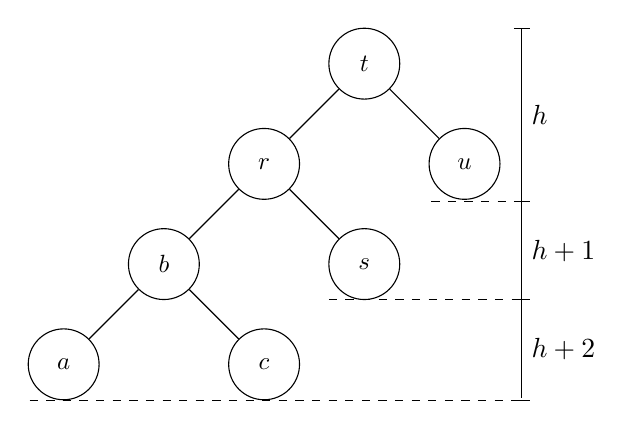
\begin{tikzpicture}[baseline={(0,0)},node distance={20mm},main/.style={draw, circle, scale=0.9, minimum size=10mm}]
    \node[main] (0) {$t$};

    \node[main] (1) [below left of=0] {$r$};
    \node[main] (2) [below right of=0] {$u$};

    \node[main] (3) [below left of=1] {$b$};
    \node[main] (4) [below right of=1] {$s$};

    \node[main] (5) [below left of=3] {$a$};
    \node[main] (6) [below right of=3] {$c$};

    \draw (0) -- (1);
    \draw (0) -- (2);
    \draw (1) -- (3);
    \draw (1) -- (4);
    \draw (3) -- (5);
    \draw (3) -- (6);

    \draw (2,0.45) -- (2,-1.75) node[midway, right] {$h$};
    \draw (1.9,0.45) -- (2.1,0.45);
    \draw [dashed] (0.85,-1.75) -- (1.9,-1.75);
    \draw (1.9,-1.75) -- (2.1,-1.75);
    \draw (2,-1.75) -- (2,-3) node[midway, right] {$h+1$};
    \draw [dashed] (-0.45,-3) -- (1.9,-3);
    \draw (1.9,-3) -- (2.1,-3);
    \draw (2,-3) -- (2,-4.25) node[midway, right] {$h+2$};
    \draw [dashed] (-4.25,-4.275) -- (1.9,-4.275);
    \draw (1.9,-4.275) -- (2.1, -4.275);
\end{tikzpicture} &
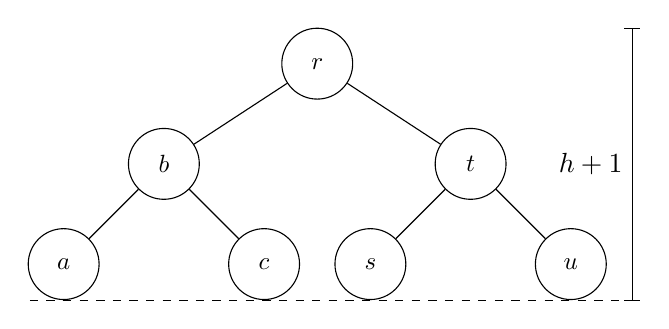
\begin{tikzpicture}[baseline={(0,0)},node distance={20mm},main/.style={draw, circle, scale=0.9, minimum size=10mm}]
    \node[main] (1) [] {$r$};

    \node[main] (0) [below right of=1, xshift=7.5mm] {$t$};
    \node[main] (2) [below right of=0] {$u$};

    \node[main] (3) [below left of=1, xshift=-7.5mm] {$b$};
    \node[main] (4) [below left of=0] {$s$};

    \node[main] (5) [below left of=3] {$a$};
    \node[main] (6) [below right of=3] {$c$};

    \draw (0) -- (1);
    \draw (0) -- (2);
    \draw (1) -- (3);
    \draw (0) -- (4);
    \draw (3) -- (5);
    \draw (3) -- (6);

    \draw (4,0.45) -- (4,-3) node[midway, left] {$h+1$};
    \draw (3.9,0.45) -- (4.1,0.45);
    \draw [dashed] (-3.65,-3.01) -- (3.9,-3.01);
    \draw (3.9,-3.01) -- (4.1,-3.01);
\end{tikzpicture}
\end{tabular}
\caption{Esempio di \emph{rotazione verso destra} del \emph{nodo} $t$}
\end{figure}

\begin{code}{Implementazione funzioni di rotazione}
\begin{minipage}[t]{0.48\textwidth}
    \com{Rotazione verso sinistra}
    \rmbreak\ind\bc{TREE} rotateLeft(\bc{TREE} r)\\
        \bc{TREE} s = r.right\\
        \bc{TREE} t = r.parent\\
        \nl\rmbreak\ind\\
        \com{Il \emph{sottoalbero sinistro} di $s$}
        \com{diventa il \emph{figlio destro} di $r$}
        r.right = s.left\\
        \indf if (s.left $\neq$ nil) then\\
            s.left.parent = r\\
        \nl\rmbreak\ind\\
        \com{$r$ diventa il \emph{figlio sinistro}}
        \com{di $s$}
        s.left = r\\
        r.parent = s\\

        \nl\rmbreak\ind\\
        \com{$s$ diventa il \emph{figlio} di $t$}
        s.parent = t\\
        \indf if (t $\neq$ nil) then\\
            \indff if (t.left == r) then\\
                t.left = s\\
            \indff else\\
                t.right = s\\
        \indf return s\\
\end{minipage}
\hfill
\begin{minipage}[t]{0.48\textwidth}
    \com{Rotazione verso destra}
    \rmbreak\ind\bc{TREE} rotateRight(\bc{TREE} r)\\
        \bc{TREE} b = r.left\\
        \bc{TREE} t = r.parent\\
        \nl\rmbreak\ind\\
        \com{Il \emph{sottoalbero destro} di $b$}
        \com{diventa il \emph{figlio sinistro} di $r$}
        r.left = b.right\\
        \indf if (b.right $\neq$ nil) then\\
            b.right.parent = r\\
        \nl\rmbreak\ind\\
        \com{$r$ diventa il \emph{figlio destro}}
        \com{di $b$}
        b.right = r\\
        r.parent = b\\

        \nl\rmbreak\ind\\
        \com{$b$ diventa il \emph{figlio} di $t$}
        b.parent = t\\
        \indf if (t $\neq$ nil) then\\
            \indff if (t.left == r) then\\
                t.left = b\\
            \indff else\\
                t.right = b\\
        \indf return b\\
\end{minipage}
\end{code}

\begin{figure}[h!]
\centering
\begin{tabular}[t]{c@{\quad}|@{\quad}c}
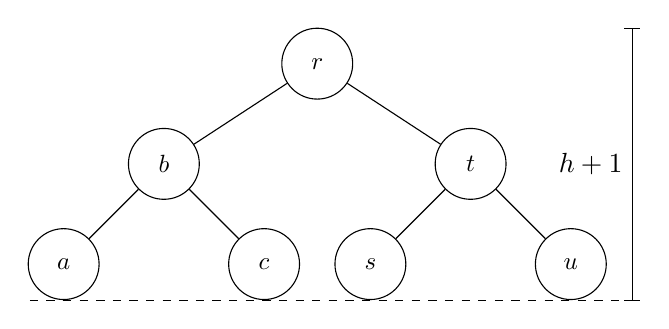
\begin{tikzpicture}[baseline={(0,0)},node distance={20mm},main/.style={draw, circle, scale=0.9, minimum size=10mm}]
    \node[main] (1) [] {$r$};

    \node[main] (0) [below right of=1, xshift=7.5mm] {$t$};
    \node[main] (2) [below right of=0] {$u$};

    \node[main] (3) [below left of=1, xshift=-7.5mm] {$b$};
    \node[main] (4) [below left of=0] {$s$};

    \node[main] (5) [below left of=3] {$a$};
    \node[main] (6) [below right of=3] {$c$};

    \draw (0) -- (1);
    \draw (0) -- (2);
    \draw (1) -- (3);
    \draw (0) -- (4);
    \draw (3) -- (5);
    \draw (3) -- (6);

    \draw (4,0.45) -- (4,-3) node[midway, left] {$h+1$};
    \draw (3.9,0.45) -- (4.1,0.45);
    \draw [dashed] (-3.65,-3.01) -- (3.9,-3.01);
    \draw (3.9,-3.01) -- (4.1,-3.01);
\end{tikzpicture} &
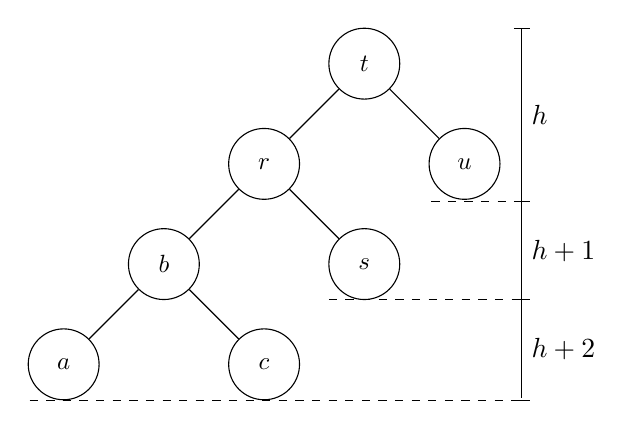
\begin{tikzpicture}[baseline={(0,0)},node distance={20mm},main/.style={draw, circle, scale=0.9, minimum size=10mm}]
    \node[main] (0) {$t$};

    \node[main] (1) [below left of=0] {$r$};
    \node[main] (2) [below right of=0] {$u$};

    \node[main] (3) [below left of=1] {$b$};
    \node[main] (4) [below right of=1] {$s$};

    \node[main] (5) [below left of=3] {$a$};
    \node[main] (6) [below right of=3] {$c$};

    \draw (0) -- (1);
    \draw (0) -- (2);
    \draw (1) -- (3);
    \draw (1) -- (4);
    \draw (3) -- (5);
    \draw (3) -- (6);

    \draw (2,0.45) -- (2,-1.75) node[midway, right] {$h$};
    \draw (1.9,0.45) -- (2.1,0.45);
    \draw [dashed] (0.85,-1.75) -- (1.9,-1.75);
    \draw (1.9,-1.75) -- (2.1,-1.75);
    \draw (2,-1.75) -- (2,-3) node[midway, right] {$h+1$};
    \draw [dashed] (-0.45,-3) -- (1.9,-3);
    \draw (1.9,-3) -- (2.1,-3);
    \draw (2,-3) -- (2,-4.25) node[midway, right] {$h+2$};
    \draw [dashed] (-4.25,-4.275) -- (1.9,-4.275);
    \draw (1.9,-4.275) -- (2.1, -4.275);
\end{tikzpicture}
\end{tabular}
\caption{Esempio di \emph{rotazione verso sinistra} del \emph{nodo} $t$}
\end{figure}\noindent
Da questo esempio si vede anche che applicando una rotazione su un \emph{nodo}
e applicando poi la rotazione inversa sullo stesso \emph{nodo}, si riottiene
l'\emph{albero} di partenza della prima rotazione.

\subsection{Inserimento}
A questo punto, possiamo affrontare l'argomento \emph{inserimento}, che nei
principi generali non si discosta molto da quanto visto per gli \emph{alberi
binari di ricerca}. In particolare, la posizione di inserimento viene
ricercata con le stesse regole, ma in più il nuovo \emph{nodo} viene \q{colorato}
di rosso.

\noindent
Ovviamente, come già accennato, l'inserimento di un \emph{nodo} può comportare
la violazione dei \emph{vincoli di bilanciamento}. È quindi opportuno che ad
ogni inserimento, se necessario, l'\emph{albero} venga ribilanciato.

\begin{minicode}{Implementazione insertNode per Alberi Red-Black}
\ind\bc{TREE} insertNode(\bc{TREE} t, \bc{ITEM} k, \bc{ITEM} v)\\
    \bc{TREE} p = nil\hfill\com{Riferimento al \emph{padre}}
    \bc{TREE} u = t\\
    \indf while (u $\neq$ nil and u.key $\neq$ k) do\hfill\com{Cerca la posizione di inserimento}
        p = u\\
        u = iif(k < u.key, u.left, u.right)\\
    \indf if (u $\neq$ nil and u.key == k) then\hfill\com{Chiave già presente}
        u.value = v\\
    \indf else\\
        \bc{TREE} newTree = Tree(k, v)\hfill\com{Crea un nuovo \emph{nodo}}
        link(p, newTree, k)\hfill\com{Inserisce il nuovo \emph{nodo}}
        balanceInsert(newTree)\hfill\com{Garantisce il bilanciamento dell'\emph{albero}}
        \indff if (p == nil) then\hfill\com{Il \emph{nodo} creato è il primo dell'\emph{albero}}
            t = newTree\\
    \indf return t
\end{minicode}\noindent
La funzione \texttt{balanceInsert} si occupa di garantire il rispetto di tutti i
\emph{vincoli di bilanciamento} modificando la colorazione dei \emph{nodi} o
applicando delle rotazioni.

Questa funzione procede con un approccio bottom-up a partire dal \emph{nodo}
inserito. A mano a mano che risale, i \emph{figli} di ogni \emph{nodo} rosso
vengono colorati di nero, garantendo così il rispetto del \emph{vincolo 3}.
Tutte le violazioni ancora irrisolte vengono in questo modo spostate verso
l'alto. Quando infine viene raggiunta la \emph{radice}, questa viene colorata
di nero come richiesto dal \emph{vincolo 1}, ma ciò si rende necessario solo se
il \emph{nodo} inserito era proprio la \emph{radice} o se risalendo
l'\emph{albero} era stata colorata di rosso.

\begin{note}
    Le operazioni di ripristino sono necessarie solo quando due \emph{nodi}
    consecutivi sono rossi.
\end{note}
\begin{note}
    Ogni \emph{nodo} inserito viene in automatico colorato di rosso perché in
    questo modo c'è la possibilità che non sia necessario ribilanciare
    l'\emph{albero}. Al contrario, l'inserimento di un \emph{nodo} nero
    comporta sempre un ribilanciamento perché viene modificata
    l'\emph{altezza nera} dell'\emph{albero}.
\end{note}

\medskip\noindent
\begin{minipage}[c]{0.6\textwidth}
Quando si inserisce un \emph{nodo}, per capire se i \emph{vincoli di bilanciamento}
sono stati violati, è sufficiente analizzare quattro \emph{nodi}:
\begin{itemize}
    \item Il \emph{nodo} $t$ appena inserito;
    \item Il \emph{padre} $p$ di $t$;
    \item Il \emph{padre} $n$ di $p$ o, equivalentemente, il \emph{nonno} di $t$;
    \item Il secondo \emph{figlio} $z$ di $n$, ovvero il \emph{fratello} di $p$ o
    lo \emph{zio} di $t$;
\end{itemize}
\end{minipage}
\hfill
\begin{minipage}[c]{0.38\textwidth}
\begin{center}
\begin{tikzpicture}[node distance={20mm},main/.style={draw, circle, scale=1, minimum size=10mm}]
    \node[main] (0) {$n$};
    \node[main] (1) [below left of=0] {$p$};
    \node[main] (2) [below right of=0] {$z$};
    \node[main] (3) [below left of=1] {$t$};

    \draw (0) -- (1);
    \draw (0) -- (2);
    \draw (1) -- (3);
\end{tikzpicture}
\end{center}
\end{minipage}

\medskip\noindent
A seconda del colore di questi quattro \emph{nodi} si configurano 7 possibili
casi.

\paragraph{Caso 1 - Il nuovo nodo non ha padre}
Questo caso si configura quando viene inserita la \emph{radice} dell'\emph{albero}
o quando risalendo si è arrivati alla \emph{radice}. A questo punto l'unico
vincolo che potrebbe risultare violato è il numero 1, quindi è sufficiente
colorare il \emph{nodo} di nero.

\begin{figure}[ht]
    \centering
    \begin{graph}
        \tikzset{rb/.style={main, font=\large\boldmath}}
        \tikzset{b/.style={rb, fill=black, color=black, text=red}}
        \tikzset{r/.style={rb, fill=red, color=red, text=black}}
        \tikzset{nil/.style={rectangle, fill=black, color=black, text=red, font=\ttfamily\large}}
    
        \node[r] (0) {$t$};
        \node[main] (1) [below left of=0] {};
        \node[main] (2) [below right of=0] {};
        \node[] (l1) [left of=0] {$(1)$};
        \node[] (l2) [right of=0, xshift=20] {\Huge$\Longrightarrow$};
    
        \node[b] (3) [right of=l2, xshift=20] {$t$};
        \node[] (l3) [right of=3] {$t=\texttt{nil}$};
        \node[main] (4) [below left of=3] {};
        \node[main] (5) [below right of=3] {};
    
        \node[inner sep=0] (6) [below left of=1, xshift=15, yshift=-20] {};
        \node[inner sep=0] (7) [below right of=1, xshift=-15, yshift=-20] {};
        \node[inner sep=0] (8) [below left of=2, xshift=15, yshift=-20] {};
        \node[inner sep=0] (9) [below right of=2, xshift=-15, yshift=-20] {};
    
        \node[inner sep=0] (10) [below left of=4, xshift=15, yshift=-20] {};
        \node[inner sep=0] (11) [below right of=4, xshift=-15, yshift=-20] {};
        \node[inner sep=0] (12) [below left of=5, xshift=15, yshift=-20] {};
        \node[inner sep=0] (13) [below right of=5, xshift=-15, yshift=-20] {};
    
        \path[-]  (0)   edge (1)
                  (0)   edge (2)
                  (3)   edge (4)
                  (3)   edge (5)
                  (1)   edge (6)
                  (1)   edge (7)
                  (2)   edge (8)
                  (2)   edge (9)
                  (4)   edge (10)
                  (4)   edge (11)
                  (5)   edge (12)
                  (5)   edge (13)
                  (6)   edge node[midway, above, yshift=10] {$A$} (7)
                  (8)   edge node[midway, above, yshift=10] {$B$} (9)
                  (10)  edge node[midway, above, yshift=10] {$A$} (11)
                  (12)  edge node[midway, above, yshift=10] {$B$} (13);
      \end{graph}
    \caption{Risoluzione del caso 1}
\end{figure}

\paragraph{Caso 2 - Il padre di \bm{$t$} è nero}
In questo caso non serve fare nulla, poiché nessun vincolo può risultare violato.

\begin{figure}[h!]
    \centering
    \begin{graph}
        \tikzset{rb/.style={main, font=\large\boldmath}}
        \tikzset{b/.style={rb, fill=black, color=black, text=red}}
        \tikzset{r/.style={rb, fill=red, color=red, text=black}}
        \tikzset{nil/.style={rectangle, fill=black, color=black, text=red, font=\ttfamily\large}}
    
        \node[r] (0) {$t$};
        \node[b] (1) [below left of=0] {};
        \node[b] (2) [below right of=0] {};
        \node[] (l1) [left of=0] {$(2)$};
    
        \node[b] (3) [above right of=0, xshift=20] {$p$};
        \node[main] (4) [below right of=3, xshift=20] {};
        \node[] (l2) [right of=3, xshift=40] {$t=\texttt{nil}$};
        \node[] (l3) [right of=4, xshift=-20] {$(Ok)$};
    
        \node[inner sep=0] (6) [below left of=1, xshift=15, yshift=-20] {};
        \node[inner sep=0] (7) [below right of=1, xshift=-15, yshift=-20] {};
        \node[inner sep=0] (8) [below left of=2, xshift=15, yshift=-20] {};
        \node[inner sep=0] (9) [below right of=2, xshift=-15, yshift=-20] {};
    
        \node[inner sep=0] (10) [below left of=4, xshift=15, yshift=-20] {};
        \node[inner sep=0] (11) [below right of=4, xshift=-15, yshift=-20] {};
    
        \path[-]  (0)   edge (1)
                  (0)   edge (2)
                  (0)   edge (3)
                  (3)   edge (4)
                  (1)   edge (6)
                  (1)   edge (7)
                  (2)   edge (8)
                  (2)   edge (9)
                  (4)   edge (10)
                  (4)   edge (11)
                  (6)   edge node[midway, above, yshift=10] {$A$} (7)
                  (8)   edge node[midway, above, yshift=10] {$B$} (9)
                  (10)  edge node[midway, above, yshift=10] {$C$} (11);
    \end{graph}
    \caption{Risoluzione del caso 2}
\end{figure}

\paragraph{Caso 3 - Sia \bm{$t$} che il padre e lo zio sono rossi}
Poiché $z$ è rosso, è possibile colorare di nero $p$ e $z$ e poi colorare di
rosso $n$. A questo punto, poiché tutti i cammini che passano per $p$ e $z$
passano anche per $n$, l'\emph{altezza nera} certamente non avrà subito variazioni.

A questo punto, è ancora possibile che $n$ violi i \emph{vincoli 1} e \emph{3}.
Di conseguenza, risaliamo l'\emph{albero} ponendo $t=n$ e ripetiamo il ciclo.

\begin{figure}[h!]
    \centering
    \resizebox*{\textwidth}{!}{
    \begin{graph}
        \tikzset{rb/.style={main, font=\large\boldmath}}
        \tikzset{b/.style={rb, fill=black, color=black, text=red}}
        \tikzset{r/.style={rb, fill=red, color=red, text=black}}
        \tikzset{nil/.style={rectangle, fill=black, color=black, text=red, font=\ttfamily\large}}

        \node[r] (0) {$t$};
        \node[b] (1) [below left of=0, xshift=10] {};
        \node[b] (2) [below right of=0, xshift=-10] {};
        \node[] (l1) [left of=0] {$(3)$};

        \node[r] (3) [above right of=0, xshift=0] {$p$};
        \node[b] (4) [below right of=3, xshift=0] {};

        \node[b] (5) [above right of=3, xshift=30] {$n$};

        \node[inner sep=0] (6) [below left of=1, xshift=15, yshift=-20] {};
        \node[inner sep=0] (7) [below right of=1, xshift=-15, yshift=-20] {};
        \node[inner sep=0] (8) [below left of=2, xshift=15, yshift=-20] {};
        \node[inner sep=0] (9) [below right of=2, xshift=-15, yshift=-20] {};

        \node[inner sep=0] (10) [below left of=4, xshift=15, yshift=-20] {};
        \node[inner sep=0] (11) [below right of=4, xshift=-15, yshift=-20] {};

        \node[r] (12) [below right of=5, xshift=30] {$z$};
        \node[b] (13) [below left of=12, xshift=0] {};
        \node[b] (14) [below right of=12, xshift=0] {};

        \node[inner sep=0] (15) [below left of=13, xshift=15, yshift=-20] {};
        \node[inner sep=0] (16) [below right of=13, xshift=-15, yshift=-20] {};
        \node[inner sep=0] (17) [below left of=14, xshift=15, yshift=-20] {};
        \node[inner sep=0] (18) [below right of=14, xshift=-15, yshift=-20] {};

        \path[-]  (0)   edge (1)
                (0)   edge (2)
                (0)   edge (3)
                (3)   edge (4)
                (3)   edge (5)
                (1)   edge (6)
                (1)   edge (7)
                (2)   edge (8)
                (2)   edge (9)
                (4)   edge (10)
                (4)   edge (11)
                (5)   edge (12)
                (12)  edge (13)
                (12)  edge (14)
                (13)  edge (15)
                (13)  edge (16)
                (14)  edge (17)
                (14)  edge (18)
                (6)   edge node[midway, above, yshift=10] {$A$} (7)
                (8)   edge node[midway, above, yshift=10] {$B$} (9)
                (10)  edge node[midway, above, yshift=10] {$C$} (11)
                (15)  edge node[midway, above, yshift=10] {$D$} (16)
                (17)  edge node[midway, above, yshift=10] {$E$} (18);
        
        \node[] (l2) [right of=12, xshift=30] {\Huge$\Longrightarrow$};

        \node[b] (23) [right of=l2, xshift=30] {$p$};
        \node[b] (24) [below right of=23, xshift=0] {};

        \node[r] (20) [below left of=23] {$t$};
        \node[b] (21) [below left of=20, xshift=10] {};
        \node[b] (22) [below right of=20, xshift=-10] {};

        \node[r] (25) [above right of=23, xshift=30] {$n$};

        \node[inner sep=0] (26) [below left of=21, xshift=15, yshift=-20] {};
        \node[inner sep=0] (27) [below right of=21, xshift=-15, yshift=-20] {};
        \node[inner sep=0] (28) [below left of=22, xshift=15, yshift=-20] {};
        \node[inner sep=0] (29) [below right of=22, xshift=-15, yshift=-20] {};

        \node[inner sep=0] (30) [below left of=24, xshift=15, yshift=-20] {};
        \node[inner sep=0] (31) [below right of=24, xshift=-15, yshift=-20] {};

        \node[b] (32) [below right of=25, xshift=30] {$z$};
        \node[b] (33) [below left of=32, xshift=0] {};
        \node[b] (34) [below right of=32, xshift=0] {};

        \node[inner sep=0] (35) [below left of=33, xshift=15, yshift=-20] {};
        \node[inner sep=0] (36) [below right of=33, xshift=-15, yshift=-20] {};
        \node[inner sep=0] (37) [below left of=34, xshift=15, yshift=-20] {};
        \node[inner sep=0] (38) [below right of=34, xshift=-15, yshift=-20] {};

        \node[] (l3) [right of=25, xshift=40] {$t=n$};

        \path[-]  (20)  edge (21)
                (20)  edge (22)
                (20)  edge (23)
                (23)  edge (24)
                (23)  edge (25)
                (21)  edge (26)
                (21)  edge (27)
                (22)  edge (28)
                (22)  edge (29)
                (24)  edge (30)
                (24)  edge (31)
                (25)  edge (32)
                (32)  edge (33)
                (32)  edge (34)
                (33)  edge (35)
                (33)  edge (36)
                (34)  edge (37)
                (34)  edge (38)
                (26)  edge node[midway, above, yshift=10] {$A$} (27)
                (28)  edge node[midway, above, yshift=10] {$B$} (29)
                (30)  edge node[midway, above, yshift=10] {$C$} (31)
                (35)  edge node[midway, above, yshift=10] {$D$} (36)
                (37)  edge node[midway, above, yshift=10] {$E$} (38);
    \end{graph}}
    \caption{Risoluzione del caso 3}
\end{figure}

\newpage
\paragraph{Caso 4 - Sia \bm{$t$} che il padre sono rossi e lo zio è nero}
\begin{enumerate}[label=\alph*.]
    \item \emph{$t$ è il figlio destro di $p$ e $p$ è il figlio sinistro di $n$}:
    viene eseguita una rotazione verso sinistra partendo dal \emph{nodo} $p$ in
    modo da rendere $p$ il \emph{figlio sinistro} di $t$ e potersi così ricondurre
    al \emph{caso 5a}. In questo caso vengono coinvolti soltanto i \emph{nodi}
    $p$ e $t$ che essendo entrambi rossi, non influenzano l'\emph{altezza nera};
    \item \emph{$t$ è il figlio sinistro di $p$ e $p$ è il figlio destro di $n$}:
    viene eseguita una rotazione verso destra partendo dal \emph{nodo} $p$ in
    modo da rendere $p$ il \emph{figlio destro} di $t$ e potersi così ricondurre
    al \emph{caso 5b}. In questo caso vengono coinvolti soltanto i \emph{nodi}
    $p$ e $t$ che essendo entrambi rossi, non influenzano l'\emph{altezza nera};
\end{enumerate}

\begin{figure}[h!]
    \centering
    \resizebox*{\textwidth}{!}{
    \begin{graph}
        \tikzset{rb/.style={main, font=\large\boldmath}}
        \tikzset{b/.style={rb, fill=black, color=black, text=red}}
        \tikzset{r/.style={rb, fill=red, color=red, text=black}}
        \tikzset{nil/.style={rectangle, fill=black, color=black, text=red, font=\ttfamily\large}}

        \node[r] (0) {$t$};
        \node[b] (1) [below left of=0, xshift=10] {};
        \node[b] (2) [below right of=0, xshift=-10] {};

        \node[r] (3) [above left of=0, xshift=0] {$p$};
        \node[b] (4) [below left of=3, xshift=0] {};

        \node[b] (5) [above right of=3, xshift=40] {$n$};
        \node[] (l1) [left of=5, xshift=-10] {$\begin{array}{l}
        (4a)\\
        (4b)\text{ speculare}
        \end{array}$};

        \node[inner sep=0] (6) [below left of=1, xshift=15, yshift=-20] {};
        \node[inner sep=0] (7) [below right of=1, xshift=-15, yshift=-20] {};
        \node[inner sep=0] (8) [below left of=2, xshift=15, yshift=-20] {};
        \node[inner sep=0] (9) [below right of=2, xshift=-15, yshift=-20] {};

        \node[inner sep=0] (10) [below left of=4, xshift=15, yshift=-20] {};
        \node[inner sep=0] (11) [below right of=4, xshift=-15, yshift=-20] {};

        \node[b] (12) [below right of=5, xshift=40] {$z$};
        \node[main] (13) [below left of=12, xshift=0] {};
        \node[main] (14) [below right of=12, xshift=0] {};

        \node[inner sep=0] (15) [below left of=13, xshift=15, yshift=-20] {};
        \node[inner sep=0] (16) [below right of=13, xshift=-15, yshift=-20] {};
        \node[inner sep=0] (17) [below left of=14, xshift=15, yshift=-20] {};
        \node[inner sep=0] (18) [below right of=14, xshift=-15, yshift=-20] {};

        \path[-]  (0)   edge (1)
                (0)   edge (2)
                (0)   edge (3)
                (3)   edge (4)
                (3)   edge (5)
                (1)   edge (6)
                (1)   edge (7)
                (2)   edge (8)
                (2)   edge (9)
                (4)   edge (10)
                (4)   edge (11)
                (5)   edge (12)
                (12)  edge (13)
                (12)  edge (14)
                (13)  edge (15)
                (13)  edge (16)
                (14)  edge (17)
                (14)  edge (18)
                (6)   edge node[midway, above, yshift=10] {$B$} (7)
                (8)   edge node[midway, above, yshift=10] {$C$} (9)
                (10)  edge node[midway, above, yshift=10] {$A$} (11)
                (15)  edge node[midway, above, yshift=10] {$D$} (16)
                (17)  edge node[midway, above, yshift=10] {$E$} (18);
        
        \node[] (l2) [right of=12, xshift=40] {\Huge$\Longrightarrow$};

        \node[r] (23) [right of=l2, xshift=40] {$t$};
        \node[b] (24) [below right of=23, xshift=0] {};

        \node[r] (20) [below left of=23] {$p$};
        \node[b] (21) [below left of=20, xshift=10] {};
        \node[b] (22) [below right of=20, xshift=-10] {};

        \node[b] (25) [above right of=23, xshift=30] {$n$};

        \node[inner sep=0] (26) [below left of=21, xshift=15, yshift=-20] {};
        \node[inner sep=0] (27) [below right of=21, xshift=-15, yshift=-20] {};
        \node[inner sep=0] (28) [below left of=22, xshift=15, yshift=-20] {};
        \node[inner sep=0] (29) [below right of=22, xshift=-15, yshift=-20] {};

        \node[inner sep=0] (30) [below left of=24, xshift=15, yshift=-20] {};
        \node[inner sep=0] (31) [below right of=24, xshift=-15, yshift=-20] {};

        \node[b] (32) [below right of=25, xshift=30] {$z$};
        \node[main] (33) [below left of=32, xshift=0] {};
        \node[main] (34) [below right of=32, xshift=0] {};

        \node[inner sep=0] (35) [below left of=33, xshift=15, yshift=-20] {};
        \node[inner sep=0] (36) [below right of=33, xshift=-15, yshift=-20] {};
        \node[inner sep=0] (37) [below left of=34, xshift=15, yshift=-20] {};
        \node[inner sep=0] (38) [below right of=34, xshift=-15, yshift=-20] {};

        \node[] (l3) [right of=25, xshift=40] {$t=p$};

        \path[-]  (20)  edge (21)
                (20)  edge (22)
                (20)  edge (23)
                (23)  edge (24)
                (23)  edge (25)
                (21)  edge (26)
                (21)  edge (27)
                (22)  edge (28)
                (22)  edge (29)
                (24)  edge (30)
                (24)  edge (31)
                (25)  edge (32)
                (32)  edge (33)
                (32)  edge (34)
                (33)  edge (35)
                (33)  edge (36)
                (34)  edge (37)
                (34)  edge (38)
                (26)  edge node[midway, above, yshift=10] {$A$} (27)
                (28)  edge node[midway, above, yshift=10] {$B$} (29)
                (30)  edge node[midway, above, yshift=10] {$C$} (31)
                (35)  edge node[midway, above, yshift=10] {$D$} (36)
                (37)  edge node[midway, above, yshift=10] {$E$} (38);
    \end{graph}}
    \caption{Risoluzione del caso 4}
\end{figure}

\paragraph{Caso 5 - Sia \bm{$t$} che il padre sono rossi e lo zio è nero}
\begin{enumerate}[label=\alph*.]
    \item \emph{$t$ è il figlio sinistro di $p$ e $p$ è il figlio sinistro di $n$}:
    viene eseguita una rotazione verso destra partendo dal \emph{nodo} $n$ in modo
    da rendere $t$ ed $n$ \emph{figli} di $p$. Quindi, colorando di rosso $n$
    e di nero $p$ ci si porta in una situazione nella quale tutti i
    \emph{vincoli di bilanciamento} sono rispettati e l'\emph{altezza nera} è
    uguale alla situazione iniziale;
    \item \emph{$t$ è il figlio destro di $p$ e $p$ è il figlio destro di $n$}:
    viene eseguita una rotazione verso sinistra partendo dal \emph{nodo} $n$ in
    modo da rendere $t$ ed $n$ \emph{figli} di $p$. Quindi, colorando di rosso
    $n$ e di nero $p$ ci si porta in una situazione nella quale tutti i
    \emph{vincoli di bilanciamento} sono rispettati e l'\emph{altezza nera} è
    uguale alla situazione iniziale;
\end{enumerate}

\begin{figure}[h!]
    \centering
    \resizebox*{0.95\textwidth}{!}{
    \begin{graph}
        \tikzset{rb/.style={main, font=\large\boldmath}}
        \tikzset{b/.style={rb, fill=black, color=black, text=red}}
        \tikzset{r/.style={rb, fill=red, color=red, text=black}}
        \tikzset{nil/.style={rectangle, fill=black, color=black, text=red, font=\ttfamily\large}}

        \node[r] (0) {$t$};
        \node[b] (1) [below left of=0, xshift=10] {};
        \node[b] (2) [below right of=0, xshift=-10] {};

        \node[r] (3) [above right of=0, xshift=0] {$p$};
        \node[b] (4) [below right of=3, xshift=0] {};

        \node[b] (5) [above right of=3, xshift=40] {$n$};
        \node[] (l1) [left of=5, xshift=-10] {$\begin{array}{l}
        (5a)\\
        (5b)\text{ speculare}
        \end{array}$};

        \node[inner sep=0] (6) [below left of=1, xshift=15, yshift=-20] {};
        \node[inner sep=0] (7) [below right of=1, xshift=-15, yshift=-20] {};
        \node[inner sep=0] (8) [below left of=2, xshift=15, yshift=-20] {};
        \node[inner sep=0] (9) [below right of=2, xshift=-15, yshift=-20] {};

        \node[inner sep=0] (10) [below left of=4, xshift=15, yshift=-20] {};
        \node[inner sep=0] (11) [below right of=4, xshift=-15, yshift=-20] {};

        \node[b] (12) [below right of=5, xshift=40] {$z$};
        \node[main] (13) [below left of=12, xshift=0] {};
        \node[main] (14) [below right of=12, xshift=0] {};

        \node[inner sep=0] (15) [below left of=13, xshift=15, yshift=-20] {};
        \node[inner sep=0] (16) [below right of=13, xshift=-15, yshift=-20] {};
        \node[inner sep=0] (17) [below left of=14, xshift=15, yshift=-20] {};
        \node[inner sep=0] (18) [below right of=14, xshift=-15, yshift=-20] {};

        \path[-]  (0)   edge (1)
                (0)   edge (2)
                (0)   edge (3)
                (3)   edge (4)
                (3)   edge (5)
                (1)   edge (6)
                (1)   edge (7)
                (2)   edge (8)
                (2)   edge (9)
                (4)   edge (10)
                (4)   edge (11)
                (5)   edge (12)
                (12)  edge (13)
                (12)  edge (14)
                (13)  edge (15)
                (13)  edge (16)
                (14)  edge (17)
                (14)  edge (18)
                (6)   edge node[midway, above, yshift=10] {$B$} (7)
                (8)   edge node[midway, above, yshift=10] {$C$} (9)
                (10)  edge node[midway, above, yshift=10] {$A$} (11)
                (15)  edge node[midway, above, yshift=10] {$D$} (16)
                (17)  edge node[midway, above, yshift=10] {$E$} (18);
        
        \node[] (l2) [right of=12, xshift=40] {\Huge$\Longrightarrow$};

        \node[r] (23) [right of=l2, xshift=40] {$t$};
        \node[b] (24) [below right of=23, xshift=0] {};

        \node[b] (20) [below left of=23] {};

        \node[b] (25) [above right of=23, xshift=30] {$p$};

        \node[inner sep=0] (26) [below left of=20, xshift=15, yshift=-20] {};
        \node[inner sep=0] (27) [below right of=20, xshift=-15, yshift=-20] {};
        \node[inner sep=0] (28) [below left of=22, xshift=15, yshift=-20] {};
        \node[inner sep=0] (29) [below right of=22, xshift=-15, yshift=-20] {};

        \node[inner sep=0] (30) [below left of=24, xshift=15, yshift=-20] {};
        \node[inner sep=0] (31) [below right of=24, xshift=-15, yshift=-20] {};

        \node[r] (32) [below right of=25, xshift=30] {$n$};
        \node[b] (33) [below left of=32, xshift=0] {};
        \node[b] (34) [below right of=32, xshift=0] {$z$};

        \node[inner sep=0] (35) [below left of=33, xshift=15, yshift=-20] {};
        \node[inner sep=0] (36) [below right of=33, xshift=-15, yshift=-20] {};
        \node[main] (37) [below left of=34, xshift=10, yshift=-20] {};
        \node[main] (38) [below right of=34, xshift=-10, yshift=-20] {};

        \node[inner sep=0] (39) [below left of=37, xshift=15, yshift=-20] {};
        \node[inner sep=0] (40) [below right of=37, xshift=-15, yshift=-20] {};
        \node[inner sep=0] (41) [below left of=38, xshift=15, yshift=-20] {};
        \node[inner sep=0] (42) [below right of=38, xshift=-15, yshift=-20] {};

        \node[] (l3) [right of=25, xshift=40] {$t=\texttt{nil}$};

        \path[-]  (20)  edge (26)
                (20)  edge (27)
                (20)  edge (23)
                (23)  edge (24)
                (23)  edge (25)
                (24)  edge (30)
                (24)  edge (31)
                (25)  edge (32)
                (32)  edge (33)
                (32)  edge (34)
                (33)  edge (35)
                (33)  edge (36)
                (34)  edge (37)
                (34)  edge (38)
                (37)  edge (39)
                (37)  edge (40)
                (38)  edge (41)
                (38)  edge (42)
                (26)  edge node[midway, above, yshift=10] {$A$} (27)
                (30)  edge node[midway, above, yshift=10] {$B$} (31)
                (35)  edge node[midway, above, yshift=10] {$C$} (36)
                (39)  edge node[midway, above, yshift=10] {$D$} (40)
                (41)  edge node[midway, above, yshift=10] {$E$} (42);
    \end{graph}}
    \caption{Risoluzione del caso 5}
\end{figure}

\begin{minicode}{Implementazione balanceInsert}
\ind balanceInsert(\bc{TREE} t)\\
    t.color = RED\hfill\com{Il \emph{nodo} inserito viene inizialmente colorato di rosso}
    \indf while (t $\neq$ nil) do\\
        \bc{TREE} p = t.parent\hfill\com{\emph{Padre}}
        \bc{TREE} n = iif(p $\neq$ nil, p.parent, nil)\hfill\com{\emph{Nonno}}
        \bc{TREE} z = iif(n $\neq$ nil, iif(n.left == p, n.right, n.left), nil)\hfill\com{\emph{Zio}}
        \indff if (p == nil) then\hfill\com{Caso 1}
            t.color = BLACK\\
            t = nil\\
        \indff else if (p.color == BLACK) then\hfill\com{Caso 2}
            t = nil\\
        \indff else if (z.color == RED) then\hfill\com{Caso 3}
            p.color = BLACK\\
            z.color = BLACK\\
            n.color = RED\\
            t = n\\
        \indff else\\
            \indfff if (t == p.right and p == n.left) then\hfill\com{Caso 4a}
                rotateLeft(p)\\
                t = p\\
            \indfff else if (t == p.left and p == n.right) then\hfill\com{Caso 4b}
                rotateRight(p)\\
                t = p\\
            \indfff else\\
                \indffff if (t == p.left and p == n.left) then\hfill\com{Caso 5a}
                    rotateRight(n)\\
                \indffff else if (t == p.right and p == n.right) then\hfill\com{Caso 5b}
                    rotateLeft(n)\\
            \indfff\\
                p.color = BLACK\\
                n.color = RED\\
                t = nil
\end{minicode}

\paragraph{Complessità della balanceInsert}
Non è difficile rendersi conto che tutte le istruzione interne al ciclo
\texttt{while} hanno \emph{complessità} $O(1)$. Di conseguenza, la
\emph{complessità} totale della funzione dipende dal numero di volte che viene
eseguito il ciclo. Poiché $t$ quando viene inserito è una \emph{foglia},\footnotemark
il caso peggiore è quello in cui il ribilanciamento coinvolge tutti i \emph{livelli}
e quindi termina solo dopo aver raggiunto la \emph{radice}.
\footnotetext{I \emph{nodi} di un \emph{albero} vengono sempre inseriti al
\emph{livello} delle \emph{foglie}}

In quel caso la \emph{complessità} dipende dall'\emph{altezza} dell'\emph{albero}.
Vedremo che negli \emph{Alberi Red-Black} esiste una relazione ben precisa tra
la loro \emph{altezza} il numero di noi \emph{nodi} che contengono.
\newpage
\subsection{Altezza degli Alberi Red-Black}
\begin{definition}[Numero massimo di nodi interni]
    In un Albero Red-Black, un sottoalbero di radice $u$ contiene un numero
    $n\geq 2^{bh(u)}-1$ di nodi interni.
\end{definition}
\begin{proof}[Dimostrazione]
    Procediamo per induzione sull'altezza del nodo $u$.
    \paragraph{Caso base} Dimostro la disequazione per $h=0$:

    Se $h=0$, $u$ è una \emph{foglia} \texttt{Nil} e quindi il \emph{sottoalbero}
    con \emph{radice} $u$ non può contenere \emph{nodi interni}, quindi $n$ deve
    per forza valere $0$. Poiché:
    \[n\geq2^{bh(u)}-1=2^0-1=1-1=0\]
    ciò è confermato e quindi il caso base risulta verificato.

    \paragraph{Passo induttivo} Ipotizzo che $n\geq2^{bh(u)}-1$ per ogni
    \emph{albero} con \emph{radice} $u$ e \emph{altezza} $h\leq1$. Dimostro la
    disequazione per $h>1$:

    Se $h>1$, $u$ è certamente un \emph{nodo interno} e quindi ha due \emph{figli}.
    Ogni \emph{figlio} di $u$ ha un \emph{altezza nera} che è pari a $bh(u)$ se
    è rosso e $bh(u)-1$ se è nero. Ogni \emph{sottoalbero} con \emph{radice} uno
    dei \emph{figli} di $u$ ha \emph{altezza} $h-1$ e quindi, per ipotesi induttiva,
    so che ognuno di quei sottoalberi ha almeno $2^{bh(u)-1}-1$ \emph{nodi interni}.
    Allora, per il \emph{sottoalbero} con \emph{radice} $u$ vale:
    \[n\geq2\cdot\left(2^{bh(u)-1}-1\right)+1\]
    cioè, il numero di \emph{nodi interni} del \emph{sottoalbero} con \emph{radice}
    $u$ è pari, almeno, alla somma dei limiti inferiori al numero di \emph{nodi
    interni} dei \emph{sottoalberi} che hanno come \emph{radice} un \emph{figlio}
    di $u$, più $1$, perché bisogna contare anche il \emph{nodo} $u$ stesso.
    Poiché vale seguente catena di uguaglianze:
    \[n\geq2\cdot\left(2^{bh(u)-1}-1\right)+1=2\cdot\left(\frac{2^{bh(u)}}{2}-1
    \right)+1=2^{bh(u)}-2+1=2^{bh(u)}-1\]
    il passo induttivo risulta verificato.
\end{proof}

\begin{definition}[Quota nera minima]
    In un Albero Red-Black, almeno la metà dei nodi dalla radice a una foglia
    deve essere nera.
\end{definition}
\begin{proof}[Dimostrazione]
    Per il secondo \emph{vincolo di bilanciamento}, i \emph{figli} di un
    \emph{nodo} rosso devono essere neri e, poiché la situazione in cui sono
    presenti il minor numero di \emph{nodi} neri è quando \emph{nodi} rossi
    e neri sono alternati, almeno la metà dei \emph{nodi} devono essere neri.
\end{proof}

\begin{definition}[Lunghezza massima dei cammini semplici]
    In un Albero Red-Black, dati due cammini semplici, dalla radice a due
    foglie, non è possibile che uno sia lungo più del doppio dell'altro.
\end{definition}
\begin{proof}[Dimostrazione]
    Per il quarto \emph{vincolo di bilanciamento}, tutti i \emph{cammini} da
    un \emph{nodo} ad una \emph{foglia} hanno lo stesso numero di \emph{nodi}
    neri e, per la definizione precedente, almeno la metà di quei \emph{nodi}
    deve essere nera. Di conseguenza, il caso più sbilanciato è quello in cui
    un \emph{cammino} è costituito da soli \emph{nodi} neri e l'altro da
    \emph{nodi} neri e rossi alternati e quindi si ha che il secondo \emph{cammino}
    è lungo il doppio del primo.
\end{proof}

\begin{definition}[Altezza massima di un Albero Red-Black]
    L'altezza massima di un Albero Red-Black con $n$ nodi interni è al più
    $2\log(n+1)$.
\end{definition}
\begin{proof}[Dimostrazione]
    Vale quanto segue:
    \[n\geq2^{bh(u)}-1\begin{array}[t]{cll}
        \Leftrightarrow & n\geq2^{h/2}-1 & \quad\hyperref[def:52]{\emph{Quota nera minima}}\\
        \Leftrightarrow & n+1\geq2^{h/2}\\
        \Leftrightarrow & \log(n+1)\geq\frac{h}{2} & \quad\emph{Applicazione logaritmo ai termini}\\
        \Leftrightarrow & h\leq2\log(n+1)
    \end{array}\]
\end{proof}

\paragraph{Complessità funzione insertNode}
Fatte queste considerazioni sull'\emph{altezza} massima degli \emph{Alberi
Red-Black}, possiamo affermare che la \emph{complessità} della funzione
\texttt{insertNode} è $O(\log n)$. Questo è vero in quanto costa $O(\log n)$
discendere l'\emph{albero} dalla \emph{radice} al punto di inserimento, costa
$O(1)$ inserire il \emph{nodo} e infine, costa $O(\log n)$ ribilanciare
l'\emph{albero} nel caso peggiore, il caso 3.

\subsection{Cancellazione}
Similmente a quanto visto per l'inserimento, la funzione \texttt{removeNode} per
gli \emph{Alberi Red-Black} è costruita a partire dalla controparte per
\emph{alberi binari di ricerca} ed è costituita da un insieme di casistiche che
possono comportare o meno, la necessità di ribilanciare l'\emph{albero}.

Le operazioni di ribilanciamento si rendono necessarie soltanto quando viene
rimosso un \emph{nodo} nero. Ciò è vero in quanto l'eliminazione di un \emph{nodo}
nero comporta sicuramente una variazione dell'\emph{altezza nera} e potrebbe
anche portare ad avere due \emph{nodi} rossi in posizioni consecutive.

Più in generale, quando viene rimosso un \emph{nodo} nero possono essere violati
i \emph{vincoli} 1, 3 o 4. In particolare:
\begin{itemize}
    \item \emph{Violato il vincolo 1}: viene eliminata la \emph{radice} e la
    nuova \emph{radice} è rossa;
    \item \emph{Violato il vincolo 3}: viene eliminato un \emph{nodo} che
    aveva il \emph{padre} e almeno uno dei \emph{figli} rossi;
    \item \emph{Violato il vincolo 4}: ogni volta che viene eliminato un
    \emph{nodo} nero, l'\emph{altezza} nera cambia;
\end{itemize}

\begin{minicode}{Implementazione removeNode per Alberi Red-Black}
\ind\bc{TREE} removeNode(\bc{TREE} t, \bc{ITEM} k)\\
    \bc{TREE} u = lookupNode(t, k)\\
    \indf if (u $\neq$ nil) then\\
        \indff if (u.left == nil and u.right == nil) then\hfill\com{Caso 1}
            link(u.parent, nil, k)\hfill\com{Rimuove il \emph{figlio}}
            delete u\\
        \indff else if (u.left $\neq$ nil and u.right $\neq$ nil) then\hfill\com{Caso 3}
            \bc{TREE} s = successorNode(u)\\
            link(s.parent, s.right, s.key)\hfill\com{Attacca il \emph{figlio} di $s$ al \emph{padre} di $s$}
            u.key = s.key\hfill\com{Copia su $u$ la chiave di $s$}
            u.value = s.value\hfill\com{Copia su $u$ il valore di $s$}
            delete s
\end{minicode}
\begin{codecont}
\begin{minipage}[t]{\textwidth}
        \indff else\hfill\com{Caso 2 con \emph{figlio destro}}
            link(u.parent, u.right, k)\\
            \indfff if (u.parent == nil) then\\
                t = u.right\\
        \\\indff if (u.color == BLACK) then\\
            balanceRemove(t, u)\hfill\com{Garantisce il bilanciamento dell’albero}
    \indf return t
\end{minipage}
\end{codecont}

\begin{minicode}{Implementazione balanceRemove}
\ind balanceRemove(\bc{TREE} r, \bc{TREE} t)\\
    \indf while (t $\neq$ r and t.color == BLACK) do\hfill\com{Il ciclo termina quando $t$ diventa}
    \mbox{}\hfill\com{la \emph{radice} o un \emph{nodo} rosso}
    \bc{TREE} p = t.parent\hfill\com{\emph{Padre}}
    \indff if (t == p.left) then\hfill\com{È sicuramente diverso da \texttt{nil}}
        \bc{TREE} f = p.right\hfill\com{\emph{Fratello}}
        \bc{TREE} ns = f.left\hfill\com{\emph{Nipote sinistro}}
        \bc{TREE} nd = f.right\hfill\com{\emph{Nipote destro}}
        \indfff (f.color == RED) then\hfill\com{Caso 1}
            p.color = RED\\
            f.color = BLACK\\
            rotateLeft(p)\\
        \indfff else\\
            \indffff if (ns.color == BLACK and nd.color == BLACK) then\hfill\com{Caso 2}
                f.color = RED\\
                t = p\\
            \indffff else if (ns.color == RED and nd.color == BLACK) then\hfill\com{Caso 3}
                ns.color = BLACK\\
                f.color = RED\\
                rotateRight(f)\\
            \indffff else if (nd.color == RED) then\hfill\com{Caso 4}
                f.color = p.color\\
                p.color = BLACK\\
                nd.color = BLACK\\
                rotateLeft(p)\\
                t = r\hfill\com{Fa terminare il ciclo}
    \indff else\hfill\com{I casi si ripetono simmetrici ai precedenti}
        \dots
\end{minicode}

\paragraph{Complessità della funzione removeNode}
Come per la \texttt{insertNode} anche in questo caso la \emph{complessità}
totale è $O(\log n)$ in quanto dipende dall'\emph{altezza} dell'\emph{albero}.
\chapter{Grafi}
Moltissimi problemi possono essere visti come problemi sui \emph{grafi} e
sebbene questi abbiano forma astratta, le loro soluzioni trovano applicazioni
negli ambiti più disparati.

Abbiamo già dato una prima definizione generica di \hyperref[def:30]{\emph{grafo}},
ma adesso andremo ad estenderla introducendo una serie di concetti che saranno
necessari per affrontare proficuamente questo capitolo.

\section{Introduzione}
Diamo le seguenti definizioni.

\begin{definition}[Grafo orientato]
    Un grafo orientato è una coppia $G=(V,E)$ dove $V$ è l'insieme dei vertici,
    o dei nodi, del grafo ed $E$ è un insieme di coppie ordinate di nodi $(u,v)$
    per $u,v\in V$ dette archi, o lati.
\end{definition}
\begin{figure}[ht]
    \centering
    \resizebox*{0.44\textwidth}{!}{
      $\begin{array}[c]{rcl}
        V & = & \{\,a,b,c,d,e,f\,\}\\
        E & = & \{\,(a,b),(a,d),(d,a),\\
          &   &  \ \ (b,c),(d,c),(d,e),\\
          &   &  \ \ (e,c)\,\}
      \end{array}$
    }\hfill
    \resizebox*{0.52\textwidth}{!}{
      \begin{graph}
        \node[main] (0) {$a$};
        \node[main] (1) [above right of=0, xshift=30] {$b$};
        \node[main] (2) [below right of=0, xshift=30] {$d$};
        \node[main] (3) [right of=1, xshift=30] {$c$};
        \node[main] (4) [right of=2, xshift=30] {$e$};
        \node[main] (5) [below right of=3] {$f$};
    
        \draw[->] (0) -- (1);
        \draw[->] (0) edge[bend left=20] (2);
        \draw[<-] (0) edge[bend right=20] (2);
        \draw[->] (1) -- (3);
        \draw[->] (2) -- (3);
        \draw[->] (2) -- (4);
        \draw[->] (4) -- (3);
      \end{graph}
    }
    \caption{\emph{Grafo orientato}}
\end{figure}

\begin{definition}[Grafo non orientato]
    Un grafo non orientato è una coppia $G=(V,E)$ dove $V$ è l'insieme dei vertici,
    o dei nodi, del grafo ed $E$ è un insieme di coppie non ordinate di nodi $(u,v)$
    per $u,v\in V$ dette archi, o lati.
\end{definition}\newpage
\begin{figure}[ht]
    \centering
    \resizebox*{0.44\textwidth}{!}{
      $\begin{array}[c]{rcl}
        V & = & \{\,a,b,c,d,e,f\,\}\\
        E & = & \{\,(a,b),(a,d),(b,c),\\
          &   &  \ \ (d,c),(d,e),(e,c)\,\}
      \end{array}$
    }\hfill
    \resizebox*{0.52\textwidth}{!}{
      \begin{graph}
        \node[main] (0) {$a$};
        \node[main] (1) [above right of=0, xshift=30] {$b$};
        \node[main] (2) [below right of=0, xshift=30] {$d$};
        \node[main] (3) [right of=1, xshift=30] {$c$};
        \node[main] (4) [right of=2, xshift=30] {$e$};
        \node[main] (5) [below right of=3] {$f$};
    
        \draw (0) -- (1);
        \draw (0) -- (2);
        \draw (1) -- (3);
        \draw (2) -- (3);
        \draw (2) -- (4);
        \draw (4) -- (3);
      \end{graph}
    }
    \caption{\emph{Grafo non orientato}}
\end{figure}

\begin{note}
    I \emph{grafi orientati} e \emph{non orientati} sono anche detti,
    rispettivamente, \emph{directed} e \emph{undirected}.
\end{note}\noindent
In un \emph{grafo orientato} un \emph{vertice} $v$ è detto \emph{adiacente} a $u$
se esiste un \emph{arco} $(u,v)$ e, quell'arco, è detto \emph{incidente} da
$u$ in $v$. Ovviamente, in un \emph{grafo non orientato} la nozione di
\emph{adiacenza} è simmetrica.
\begin{eg}[Adiacenza e incidenza]
    Nel seguente grafo orientato, per la parte evidenziata, valgono le seguenti
    relazioni di adiacenza e incidenza.\\
    \begin{minipage}{0.48\textwidth}
        \centering
        \begin{graph}
            \node[main, line width=1.3pt] (0) {$a$};
            \node[main, line width=1.3pt] (1) [above right of=0, xshift=30] {$b$};
            \node[main, line width=1.3pt] (2) [below right of=0, xshift=30] {$d$};
            \node[main] (3) [right of=1, xshift=30] {$c$};
            \node[main] (4) [right of=2, xshift=30] {$e$};
            \node[main] (5) [below right of=3] {$f$};
        
            \draw[->, line width=1.3pt] (0) -- (1);
            \draw[->] (0) edge[bend left=20, line width=1.3pt] (2);
            \draw[<-] (0) edge[bend right=20, line width=1.3pt] (2);
            \draw[->] (1) -- (3);
            \draw[->] (2) -- (3);
            \draw[->] (2) -- (4);
            \draw[->] (4) -- (3);
        \end{graph}
    \end{minipage}
    \hfill
    \begin{minipage}{0.48\textwidth}
        \par\noindent
        \begin{itemize}
            \item $(a,b)$ è incidente da $a$ a $b$;
            \item $(a,d)$ è incidente da $a$ a $d$;
            \item $(d,a)$ è incidente da $d$ ad $a$;
            \item $b$ è adiacente ad $a$;
            \item $d$ è adiacente ad $a$;
            \item $a$ è adiacente a $d$;
        \end{itemize}
    \end{minipage}
\end{eg}

\subsection{Dimensioni dei grafi}
\begin{definition}[Numero di nodi e di archi]
    Dato un grafo $G=(V,E)$ il numero di nodi e il numero di archi corrispondono,
    rispettivamente, alla cardinalità degli insiemi $V$ ed $E$.
\end{definition}
\begin{note}
    Di seguito, salvo diverse indicazioni, indicheremo con $n$ il numero di
    \emph{nodi} e con $m$ il numero di \emph{archi}, cioè $n=|V|$ ed $m=|E|$.
\end{note}

\begin{definition}[Numero massimo di archi in un grafo orientato]
    Dato un grafo orientato vale la seguente relazione sul numero di
    archi:
    \[m\leq n(n-1)\]
\end{definition}
\begin{definition}[Numero massimo di archi in un grafo non orientato]
    Dato un grafo non orientato vale la seguente relazione sul numero
    di archi:
    \[m\leq\frac{n(n-1)}{2}\]
\end{definition}
\begin{note}
    In entrambi i casi possiamo affermare che il numero di \emph{archi} è $O(n^2)$.
\end{note}
\begin{note}
    Per gli algoritmi che operano sui \emph{grafi} la \emph{complessità} è espressa
    sia in termine di $n$ che $m$ e quindi considereremo \emph{lineare} un
    algoritmo con \emph{complessità} $O(n+m)$.
\end{note}

\subsection{Casi speciali}
\begin{definition}[Grafo completo]
    Un grafo con un arco tra tutte le coppie di nodi è detto completo.
\end{definition}
\begin{definition}[Grafi sparsi e densi]
    Un grafo con \q{pochi archi} è detto essere sparso, mentre uno con \q{tanti
    archi}, denso.
\end{definition}
\begin{note}
    La definizione di \emph{grafi sparsi} e \emph{densi} non è formale, ma
    tendenzialmente un \emph{grafo} con $m=O(n)$ o $O(n\log n)$ è considerato
    \emph{sparso}. Sono invece considerati \emph{densi} i \emph{grafi} con
    $m=\Omega(n^2)$.
\end{note}

\bigskip\noindent
Possiamo definire gli \emph{alberi} in funzione dei \emph{grafi}.
\begin{definition}[Albero libero]
    Un grafo con $m=n-1$ è detto albero libero.
\end{definition}
\begin{definition}[Albero radicato (visto come grafo)]
    Un grafo connesso con $m=n-1$ archi nel quale uno dei nodi è stato designato
    come radice è detto albero radicato.
\end{definition}
\begin{definition}[Foresta]
    Un insieme di alberi è detto foresta.
\end{definition}

\subsection{Cammini e gradi dei nodi}
\begin{definition}[Cammino]
    In un grafo $G=(V,E)$, una sequenza di $k+1$ nodi $u_0,\,u_1,\,\dots,\,u_k$ è
    definita essere un cammino di lunghezza $k$, se è tale per cui l'arco
    $(u_i,u_{i+1})\in E$ $\forall\,0\leq i\leq k-1$.
\end{definition}

\begin{eg}[Cammino]
\begin{minipage}{0.45\textwidth}
    \vspace{0.2cm}
    \hspace{0.2cm}
    \begin{graph}
        \node[main] (0) {$a$};
        \node[main] (1) [above right of=0, xshift=30] {$b$};
        \node[main] (2) [below right of=0, xshift=30] {$d$};
        \node[main] (3) [right of=1, xshift=30] {$c$};
        \node[main] (4) [right of=2, xshift=30] {$e$};
    
        \draw[line width=1.3pt] (0) -- (1);
        \draw[line width=1.3pt] (1) -- (3);
        \draw (2) -- (3);
        \draw[line width=1.3pt] (2) -- (4);
        \draw[line width=1.3pt] (4) -- (3);
    \end{graph}
\end{minipage}
\hfill
\begin{minipage}{0.53\textwidth}
    La sequenza di nodi $a,b,c,e,d$ è un cammino di lunghezza $4$.

    \paragraph{NB}
    In questo caso il cammino è anche detto semplice perché tutti i nodi
    che lo compongono sono distinti.
\end{minipage}
\end{eg}

\begin{definition}[Grado di un nodo in un grafo orientato]
    In un grafo orientato si definisce grado entrante di un nodo il numero di
    archi incidenti su di esso, mentre il grado uscente è definito come il numero
    di archi incidenti da esso.
\end{definition}
\begin{definition}[Grado di un nodo in un grafo non orientato]
    In un grafo non orientato il grado di un nodo è definito come il numero di
    archi incidenti su di esso.
\end{definition}

\begin{figure}[ht]
    \centering
    \subfloat[\emph{Grafo orientato}]
    {
        \resizebox*{0.48\textwidth}{!}{
            \begin{graph}
                \node[main, label={$\begin{array}{rr}
                  \emph{in} & 1\\
                  \emph{out} & 2
                \end{array}$}] (0) {$a$};
                \node[main, label={$\begin{array}{rr}
                  \emph{in} & 1\\
                  \emph{out} & 1
                \end{array}$}] (1) [above right of=0, xshift=30] {$b$};
                \node[main, label=below:{$\begin{array}{rr}
                  \emph{in} & 1\\
                  \emph{out} & 3
                \end{array}$}] (2) [below right of=0, xshift=30] {$d$};
                \node[main, label={$\begin{array}{rr}
                  \emph{in} & 3\\
                  \emph{out} & 0
                \end{array}$}] (3) [right of=1, xshift=30] {$c$};
                \node[main, label=below:{$\begin{array}{rr}
                  \emph{in} & 1\\
                  \emph{out} & 1
                \end{array}$}] (4) [right of=2, xshift=30] {$e$};
                \node[main, label={$\begin{array}{rr}
                  \emph{in} & 0\\
                  \emph{out} & 0
                \end{array}$}] (5) [below right of=3] {$f$};
            
                \draw[->] (0) -- (1);
                \draw[->] (0) edge[bend left=20] (2);
                \draw[<-] (0) edge[bend right=20] (2);
                \draw[->] (1) -- (3);
                \draw[->] (2) -- (3);
                \draw[->] (2) -- (4);
                \draw[->] (4) -- (3);
              \end{graph}
        }
    }
    \hfill
    \subfloat[\emph{Grafo non orientato}]
    {\resizebox*{0.48\textwidth}{!}{
        \begin{graph}
            \node[main, label={$2$}] (0) {$a$};
            \node[main, label={$2$}] (1) [above right of=0, xshift=30] {$b$};
            \node[main, label=below:{$3$}] (2) [below right of=0, xshift=30] {$d$};
            \node[main, label={$3$}] (3) [right of=1, xshift=30] {$c$};
            \node[main, label=below:{$2$}] (4) [right of=2, xshift=30] {$e$};
            \node[main, label={$0$}] (5) [below right of=3] {$f$};
        
            \draw (0) -- (1);
            \draw (0) -- (2);
            \draw (1) -- (3);
            \draw (2) -- (3);
            \draw (2) -- (4);
            \draw (4) -- (3);
          \end{graph}
    }}
    \caption{\emph{Grado} dei \emph{nodi} nei \emph{grafi orientati} e \emph{non orientati}}
\end{figure}

\subsection{Specifica}
\begin{code}{Grafo}
    \com{Crea un nuovo \emph{grafo}}
    \bc{GRAPH} Graph()
    \nl\com{Restituisce l'insieme di tutti i \emph{vertici}}
    \bc{SET} V()
    \nl\com{Restituisce il numero di \emph{nodi}}
    \bc{int} size()
    \nl\com{Restituisce l'insieme dei \emph{nodi adiacenti} ad $u$}
    \bc{SET} adj(\bc{NODE} u)
    \nl\com{Aggiunge un \emph{nodo} $u$ al \emph{grafo}}
    insertNode(\bc{NODE} u)
    \nl\com{Aggiunge l'\emph{arco} $(u,v)$ al \emph{grafo}}
    insertEdge(\bc{NODE} u, \bc{NODE} v)
    \nl\com{Rimuove il \emph{nodo} $u$ dal \emph{grafo}}
    removeNode(\bc{NODE} u)
    \nl\com{Rimuove l'\emph{arco} $(u,v)$ dal \emph{grafo}}
    removeEdge(\bc{NODE} u, \bc{NODE} v)
\end{code}

\subsection{Memorizzare un grafo}
Per la memorizzazione dei \emph{grafi} esistono due approcci: \emph{matrici di
adiacenza} e \emph{liste di adiacenza}.

\paragraph{Memorizzazione di un grafo orientato}
L'approccio con \emph{matrice di adiacenza} prevede che venga realizzata una
matrice $n\times n$ tale che:
\[m_{u,v}=\begin{cases}
    1 & \text{se } (u,v)\in E\\
    0 & \text{se } (u,v)\notin E
\end{cases}\]
Quindi, il \emph{grafo} viene rappresentato tramite una matrice di
valori binari nella quale la cella che si trova nell'$u$-esima riga e $v$-esima
colonna è 1 se e solo se esiste un \emph{arco} da $u$ a $v$.

D'altra parte, le \emph{liste di adiacenza} sfruttano il concetto di
\emph{adiacenza} espresso nelle specifiche dalla funzione \texttt{adj}. Vale
infatti, la seguente definizione matematica di \texttt{adj} e quindi di
\emph{adiacenza}:
\[G.adj(u)=\{v\,|\,(u,v)\in E\}\]
Quindi, nell'approccio basato su \emph{liste}, viene realizzata una \emph{lista}
contenente tutti i \emph{vertici} del \emph{grafo}. Ogni \emph{nodo} della
\emph{lista} poi, a cascata, contiene un riferimento ad un uno dei \emph{vertici}
che nel \emph{grafo} sono \emph{adiacenti} al \emph{vertice} associato a quel
\emph{nodo} della \emph{lista}.

\begin{figure}[h!]
    \centering
    \subfloat[\emph{Grafo orientato}]
    {
        \begin{graph}
            \node[main] (0) {$0$};
            \node[main] (1) [right of=0, xshift=30] {$1$};
            \node[main] (2) [below of=0, yshift=-30] {$3$};
            \node[main] (3) [right of=1, xshift=30] {$2$};
            \node[main] (4) [right of=2, xshift=30] {$4$};
            \node[main] (5) [below of=3, yshift=-30] {$5$};
        
            \draw[->] (0) -- (1);
            \draw[<-] (0) edge[bend left=20] (2);
            \draw[->] (0) edge[bend right=20] (2);
            \draw[->] (1) -- (3);
            \draw[->] (2) -- (3);
            \draw[->] (2) -- (4);
            \draw[->] (4) -- (3);
          \end{graph}
    }\\
    \subfloat[\emph{Matrice di adiacenza}]{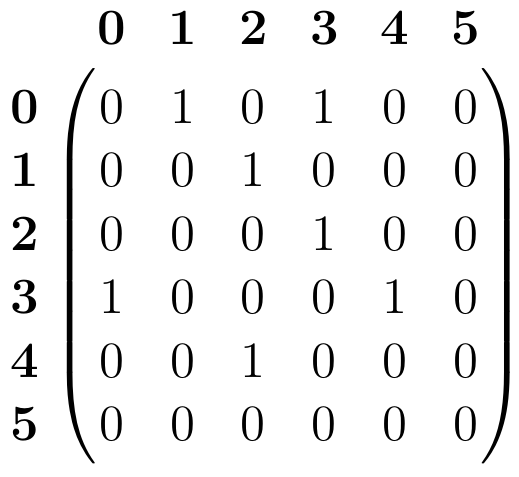
\includegraphics[width=0.48\textwidth]{matrice-di-adiacenza-esempio-1.png}}
    \hfill
    \subfloat[\emph{Lista di adiacenza}]{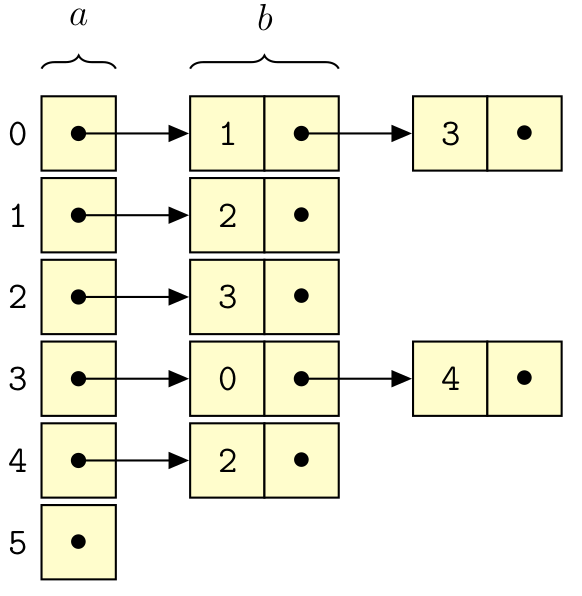
\includegraphics[width=0.48\textwidth]{lista-di-adiacenza-esempio-1.png}}
    \caption{Memorizzazione di un \emph{grafo orientato}}
\end{figure}\noindent
Dall'immagine si può derivare facilmente il \emph{costo di memorizzazione} nei
due casi. Per le \emph{matrici di adiacenza} lo spazio necessario dipende
unicamente dal quadrato del numero di \emph{nodi} e quindi è $O(n^2)$, mentre
per memorizzare una \emph{lista di adiacenza}, lo spazio usato dipende sia dal
numero di \emph{nodi} che di \emph{lati} e quindi è $O(a\cdot n+b\cdot m)=O(n+m)$.

\paragraph{Memorizzazione di un grafo non orientato}
Per i \emph{grafi non orientati} non cambia molto, ma nel caso delle
\emph{matrici di adiacenza} possiamo dimezzare lo spazio grazie alla simmetria
dell'\emph{adiacenza}. Di conseguenza lo spazio necessario diventa $O(\frac{n(n-1)}
{2})$, che però è comunque un $O(n^2)$.

Per le \emph{liste di adiacenza} invece, un \emph{arco} $(u,v)$ deve essere
memorizzato sia tra i \emph{nodi adiacenti} a $u$ che a $v$. Di conseguenza, il
numero di \emph{archi} da memorizzare raddoppia e, conseguentemente, lo spazio
necessario diventa $O(a\cdot n+2b\cdot m)$ che anche sta volte è comunque $O(n+m)$.

\begin{figure}[h!]
    \centering
    \subfloat[\emph{Grafo non orientato}]
    {
        \begin{graph}
            \node[main] (0) {$0$};
            \node[main] (1) [right of=0, xshift=30] {$1$};
            \node[main] (2) [below of=0, yshift=-30] {$3$};
            \node[main] (3) [right of=1, xshift=30] {$2$};
            \node[main] (4) [right of=2, xshift=30] {$4$};
            \node[main] (5) [below of=3, yshift=-30] {$5$};
        
            \draw (0) -- (1);
            \draw (0) -- (2);
            \draw (1) -- (3);
            \draw (2) -- (3);
            \draw (2) -- (4);
            \draw (4) -- (3);
        \end{graph}
    }\\
    \subfloat[\emph{Matrice di adiacenza}]{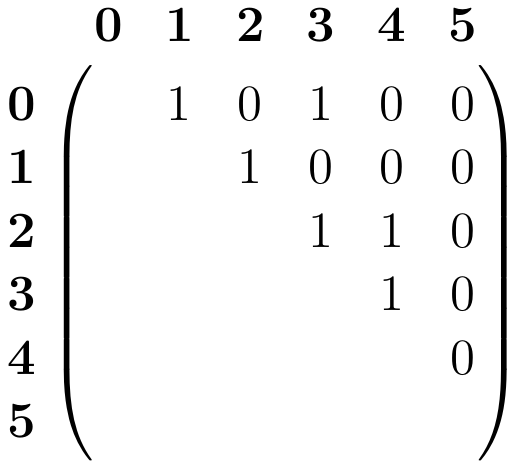
\includegraphics[width=0.48\textwidth]{matrice-di-adiacenza-esempio-1n.png}}
    \hfill
    \subfloat[\emph{Lista di adiacenza}]{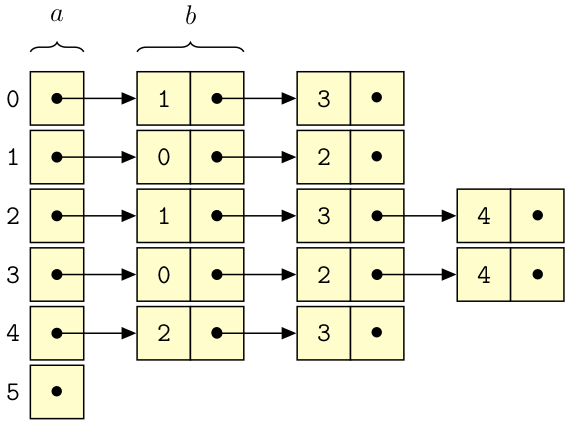
\includegraphics[width=0.48\textwidth]{lista-di-adiacenza-esempio-1n.png}}
    \caption{Memorizzazione di un \emph{grafo non orientato}}
\end{figure}\noindent
Giunti a questo punto possiamo dire che, a parità di metodo di
memorizzazione scelto, lo spazio necessario per memorizzare un \emph{grafo orientato}
non è diverso da quello che servirebbe se il \emph{grafo} fosse \emph{non orientato}.

\paragraph{Memorizzazione di un grafo pesato}
Un caso interessante è quello in cui si debba memorizzare un \emph{grafo pesato},
cioè un \emph{grafo} nel quale ad ogni \emph{arco} è associato un costo (o un
profitto). Matematicamente possiamo pensare il peso di un \emph{arco} come
l'applicazione di una funzione di peso del tipo: $w:\,V\times V\to\mathbb{R}$.
L'unico caso particolare è quello in cui non esista un \emph{arco} tra due
\emph{vertici} e quindi, a seconda del problema che si sta affrontando, si può
decidere di assegnare un peso nullo o infinito.

\noindent
Ciò che cambia nella memorizzazione è che nella \emph{matrice di adiacenza},
invece di indicare un valore binario, si indica il peso dell'\emph{arco}, mentre
nella \emph{lista di adiacenza} si aggiunge il valore del peso all'interno di
ogni \emph{nodo}.

\begin{figure}[h!]
    \centering
    \subfloat[\emph{Grafo pesato non orientato}]
    {
        \begin{graph}
            \node[main] (0) {$0$};
            \node[main] (1) [right of=0, xshift=30] {$1$};
            \node[main] (2) [below of=0, yshift=-30] {$3$};
            \node[main] (3) [right of=1, xshift=30] {$2$};
            \node[main] (4) [right of=2, xshift=30] {$4$};
            \node[main] (5) [below of=3, yshift=-30] {$5$};
        
            \draw (0) -- (1) node [midway, below] {$3$};
            \draw (0) -- (2) node [midway, right] {$1$};
            \draw (1) -- (3) node [midway, below] {$4$};
            \draw (2) -- (3) node [midway, below] {$4$};
            \draw (2) -- (4) node [midway, below] {$8$};
            \draw (4) -- (3) node [midway, below right=-1.5pt] {$7$};
        \end{graph}
    }\\
    \subfloat[\emph{Matrice di adiacenza}]{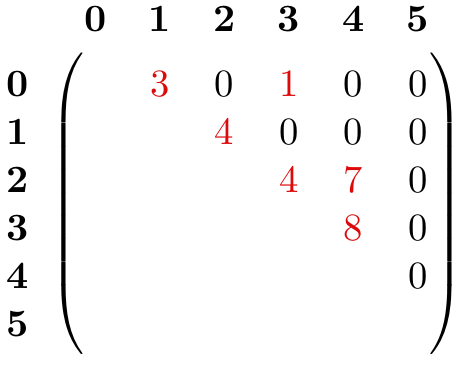
\includegraphics[width=0.48\textwidth]{matrice-di-adiacenza-esempio-1np.png}}
    \hfill
    \subfloat[\emph{Lista di adiacenza}]{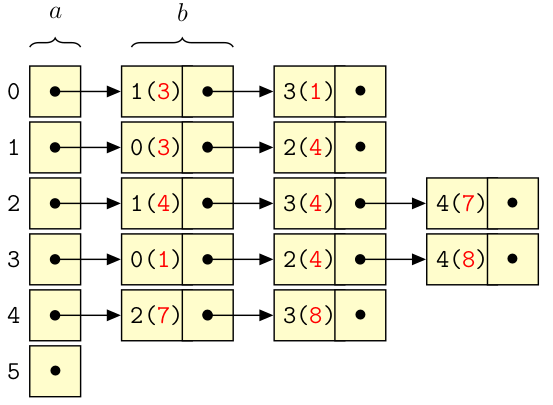
\includegraphics[width=0.48\textwidth]{lista-di-adiacenza-esempio-1np.png}}
    \caption{Memorizzazione di un \emph{grafo pesato non orientato}}
\end{figure}

\paragraph{Dettagli sull'implementazione}
Se non diversamente specificato, di seguito assumeremo che i \emph{grafi} siano
memorizzati come \emph{vettori di adiacenza}, ovvero \emph{liste} implementate
tramite \emph{vettori} (\emph{dinamici} o \emph{statici}). Inoltre, consideriamo
$O(1)$ il costo per l'accesso alle informazioni di un oggetto di classe
\texttt{NODE} e per l'inserimento e la rimozione di \emph{nodi} e \emph{archi}
dai \emph{grafi}. Ipotizzeremo inoltre, che dopo l'inizializzazione i
\emph{grafi} siano \emph{statici} e che quindi non sia più possibile modificarli.

\bigskip\noindent
Fatte queste premesse, possiamo concludere questa sezione discutendo
del \emph{costo} complessivo di alcune operazioni basilari sui \emph{grafi}.

\begin{code}{Iterazione su \emph{nodi} e \emph{archi}}
\begin{minipage}[t]{0.48\textwidth}
\com{Iterazione su tutti i \emph{nodi}}
\rmbreak\ind foreach (u $\in$ G.V()) do\\
    \{ Operazioni sul \emph{nodo} $u$ \}
\end{minipage}
\hfill
\begin{minipage}[t]{0.48\textwidth}
\com{Iterazione su tutti i \emph{nodi} e tutti gli \emph{archi}}
\rmbreak\ind foreach (u $\in$ G.V()) do\\
    \{ Operazioni sul \emph{nodo} $u$ \}\\
    \indf foreach (v $\in$ G.adj(u)) do\\
        \{ Operazioni sull'\emph{arco} $(u,v)$ \}\\
\end{minipage}
\end{code}

\noindent\begin{minipage}[t]{0.48\textwidth}
    \paragraph{Matrici di adiacenza}
    \hbadness=10000
    \begin{itemize}
        \item Lo spazio richiesto per la memorizzazione è $O(n^2)$;
        \item Il tempo richiesto per verificare se un \emph{nodo} $u$ è
        \emph{adiacente} a un altro \emph{nodo} $v$ è $O(1)$;
        \item Il tempo necessario per iterare su tutti gli \emph{archi} è $O(n^2)$
    \end{itemize}
\end{minipage}
\hfill
\begin{minipage}[t]{0.48\textwidth}
    \paragraph{Liste di adiacenza}
    \hbadness=10000
    \begin{itemize}
        \item Lo spazio richiesto per la memorizzazione è $O(n+m)$;
        \item Il tempo richiesto per verificare se un \emph{nodo} $u$ è
        \emph{adiacente} a un altro \emph{nodo} $v$ è $O(n)$;
        \item Il tempo necessario per iterare su tutti gli \emph{archi} è $O(n+m)$
    \end{itemize}
\end{minipage}

\bigskip\noindent
In generale, le \emph{matrici di adiacenza} sono adatte per memorizzare
\emph{grafi densi} e, al contrario, per \emph{grafi sparsi} risulta più
convenienti l'utilizzo delle \emph{liste}.

\section{Visite di un grafo}
\begin{definition}[Visita di un grafo]
    Dati, un grafo $G=(V,E)$ e un vertice $r\in V$ detto radice o sorgente,
    visitare un grafo significa visitare una e una sola volta tutti i nodi del
    grafo che possono essere raggiunti da $r$.
\end{definition}\noindent
Come per gli \emph{alberi}, esistono \emph{visite in profondità} e in
\emph{ampiezza}. Un primo approccio alla \emph{visita} di un \emph{grafo}
potrebbe essere il doppio ciclo visto in precedenza:
\begin{minicode}{Visita scriteriata di un grafo}
\com{Iterazione su tutti i \emph{nodi} e tutti gli \emph{archi}}
\rmbreak\ind foreach (u $\in$ G.V()) do\\
    \{ Operazioni sul \emph{nodo} $u$ \}\\
    \indf foreach (v $\in$ G.adj(u)) do\\
        \{ Operazioni sull'\emph{arco} $(u,v)$ \}
\end{minicode}\noindent
Questo approccio tuttavia non va bene in quanto non viene tenuto conto della struttura
del \emph{grafo} e, cosa più importante, non segue alcun criterio nell'ordine
di visita dei \emph{nodi} e degli \emph{archi}. A dirla tutta, questo approccio
viola la definizione stessa di \emph{visita} in quanto non offre alcuna garanzia
sul fatto che \emph{nodi} e \emph{archi} verranno visitati una sola volta.

\subsection{Visita in ampiezza}
Nella \emph{visita in ampiezza} andiamo a visitare i \emph{nodi} in ordine
crescente di distanza dalla \emph{radice}. Ciò può essere utile per calcolare
il \emph{cammino} più breve da $r$ a tutti gli altri \emph{nodi} e quindi
riuscire a generare un \emph{albero breadth-first}.
\begin{definition}[Albero breadth-first]
    Un albero breadth-first è un albero contenente tutti i nodi raggiungibili da
    $r$ e tale per cui il cammino dalla radice $r$ al nodo $u$ nell'albero
    corrisponde al cammino più breve da $r$ a $u$ nel grafo.
\end{definition}\noindent
Dunque, per l'implementazione della \emph{visita in ampiezza} possiamo partire
da quanto fatto per gli \hyperref[code:15]{\emph{alberi generici}} ipotizzando
di trattare i \emph{nodi adiacenti} come \emph{figli}. Con le opportune
modifiche si ottiene una funzione di questo tipo:
\begin{minicode}{Implementazione errata visita in ampiezza di un grafo}
\ind bfsTraversal(\bc{GRAPH} G, \bc{NODE} r)\\
    \bc{QUEUE} q = Queue()\\
    q.enqueue(r)\\
    \indf while (not q.isEmpty()) do\\
        \bc{NODE} u = q.dequeue()\\
        \{ Visita il \emph{nodo} $u$ \}\\
        \indff foreach (v $\in$ G.adj(u)) do\\
            q.enqueue(v)\hfill\com{Accoda tutti i \emph{nodi adiacenti} a $u$}
\end{minicode}\noindent
Questa implementazione, come la precedente, è errata e il motivo è che non solo
lo stesso \emph{nodo} può essere visitato più volte, ma la funzione non termina
mai l'esecuzione. Infatti, se $u$ e $v$ sono \emph{adiacenti}, quando viene
visitato $u$ viene messo in coda $v$ e quando viene visitato $v$ viene messo in
coda $u$. È quindi necessario utilizzare un sistema che permetta di tenere
traccia dei
\emph{nodi} già visitati.
\begin{minicode}{Implementazione generica visita in ampiezza di un grafo}
\ind graphTraversal(\bc{GRAPH} G, \bc{NODE} r)\\
    \bc{SET} s = Set()\hfill\com{\emph{Insieme} generico}
    s.insert(r)\hfill\com{Da specificare}
    \{ Marca il \emph{nodo} $r$ \}\\
    \indf while (s.size() > 0) do\\
        \bc{NODE} u = s.remove()\hfill\com{Da Specificare}
        \indff foreach (v $\in$ G.adj(u)) do\\
            \{ Visita l'\emph{arco} $(u,v)$ \}\\
            \indfff if (v non è stato ancora marcato) then\\
                \{ Marca il \emph{nodo} $v$ \}\\
                s.insert(v)\hfill\com{Da specificare}
\end{minicode}
\begin{code}{Implementazione visita in ampiezza di un grafo}
\noindent\rmbreak\ind bfs(\bc{GRAPH} G, \bc{NODE} r)\\
    \bc{QUEUE} q = Queue()\\
    q.enqueue(r)\\
    \bc{boolean}[] visited = new \bc{boolean}[G.size()]\hfill\com{\emph{Vettore marcatore}}
    foreach (u $\in$ G.V() - \{r\}) do\hfill\com{Estrae tutti i \emph{nodi} tranne $r$}
        \indf visited[u] = false\\
    \ind visited[r] = true\hfill\com{Marca $r$}
    \ind while (not q.isEmpty()) do\\
        \indf\bc{NODE} u = q.dequeue()\\
        \{ Visita il \emph{nodo} $u$ \}\\
        \indf foreach (v $\in$ G.adj(u)) do\\
            \indff\{ Visita l'\emph{arco} $(u,v)$ \}\\
            if (not visited[v]) then\hfill\com{Controlla se il \emph{nodo} è già stato visitato}
                \indfff visited[v] = true\hfill\com{Marca $v$}
                q.enqueue(v)
\end{code}

\subsection{Visita in profondità}
La \emph{visita in profondità} viene usata per visitare tutti i \emph{nodi} e
non solo quelli raggiungibili da una singola sorgente come avviene con la
\emph{visita in ampiezza}. Proprio per questo, la ricerca restituisce una
\emph{foresta} di \emph{alberi depth-first} e non un solo \emph{albero}.

La funzione \texttt{dfs} per la \emph{visita in profondità} può essere realizzata
in modo ricorsivo o iterativo. In entrambi i casi si fa uso di una \emph{pila},
ma nel caso della ricorsione la \emph{pila} ha una dimensione massima definita
dal sistema operativo, quindi per grafi di grandi dimensioni è bene considerare
attentamente il tipo di implementazione più opportuno.

\begin{minicode}{Implementazione ricorsiva visita in profondità di un grafo}
\ind dfs(\bc{GRAPH} G, \bc{NODE} u, \bc{boolean}[] visited)\\
    visited[u] = true\\
    \{ Visita il \emph{nodo} $u$ \}\hfill\com{Pre-order}
    \indf foreach (v $\in$ G.adj(u)) do\\
        \indff if (not visited[v]) then\\
            \{ Visita l'\emph{arco} $(u,v)$ \}\\
            dfs(G, v, visited)\\

    \indf\{ Visita il \emph{nodo} $u$ \}\hfill\com{Post-order}
\end{minicode}
\begin{minicode}{Implementazione iterativa visita in profondità di un grafo}
\ind dfs(\bc{GRAPH} G, \bc{NODE} u)\\
    \bc{STACK} s = Stack()\\
    s.push(r)\\
    \bc{boolean}[] visited = new \bc{boolean}[G.size()]\\
    \indf foreach (u $\in$ G.V()) do\\
        visited[u] = false\\
    \indf while (not s.isEmpty()) do\\
        \bc{NODE} u = s.pop()\\
        \indff if (not visited[u]) then\\
            \{ Visita il \emph{nodo} $u$ \}\hfill\com{Pre-order}
            visited[u] = true\\
            \indfff foreach (v $\in$ G.adj(u)) do\\
                \{ Visita l'\emph{arco} $(u,v)$ \}\\
                s.push(v)
\end{minicode}\noindent
È bene esplicitare alcuni particolari dell'implementazione iterativa. In
particolare, un \emph{nodo} può essere inserito più volte nella \emph{pila},
in quanto il controllo sul marcatore viene effettuato al momento dell'estrazione
e non dell'inserimento.

La \emph{visita} in \emph{post-order} prevede che alla scoperta di un \emph{nodo}, questo venga inserito nella
\emph{pila} impostando un tag \texttt{discovery}. Alla successiva estrazione di
quel \emph{nodo}, il tag \texttt{discovery} viene cambiato in \texttt{finish} e
il \emph{nodo} viene inserito nuovamente nella \emph{pila}. Alla terza
estrazione viene effettuata la \emph{visita}. L'utilizzo dei tag \texttt{discovery}
e \texttt{finish} garantisce che un \emph{nodo} con tag \texttt{finish} venga
estratto soltanto dopo che tutti i suoi vicini sono già stati inseriti.

\subsection{Complessità delle visite}
Tutte e tre le implementazioni viste per i due tipi di \emph{visite} hanno
\emph{complessità} $O(n+m)$. Nello specifico, l'implementazione iterativa della
\emph{dfs} costa $O(n+m)$ perché effettua $O(m)$ \emph{visite} degli \emph{archi},
$O(m)$ inserimenti ed estrazioni e $O(n)$ \emph{visite} dei \emph{nodi}.

\section{Problemi sui grafi risolubili con visite in ampiezza}
Le \emph{visite in ampiezza} e in \emph{profondità} sono solitamente
sfruttate all'interno di altri algoritmi per risolvere problemi più complessi.

L'utilizzo più importante delle \emph{visite in ampiezza} è nella ricerca del
\emph{cammino più breve} tra due \emph{nodi}. Tuttavia, prima di arrivare a
discutere quel problema, facciamo una piccola digressione e andiamo a vedere
come calcolare la distanza tra un \emph{nodo} e tutti gli altri.

\subsection{Calcolo della distanza tra nodi}
Per distanza tra \emph{nodi} si intende il numero di \emph{archi}
che collegano un \emph{nodo} a tutti gli altri. Il \emph{nodo} di partenza
ha distanza $0$ da se stesso, i suoi vicini, ovvero i \emph{nodi} ad esso
\emph{adiacenti}, hanno distanza $1$ e così via. In generale, se un \emph{nodo}
$u$ è \emph{adiacente} ad un \emph{nodo} che è a distanza $k$ e, contemporaneamente,
non è \emph{adiacente} a nessun \emph{nodo} che ha distanza inferiore a $k$ dal
\emph{nodo} di partenza, allora $u$ è a distanza $k+1$.

\begin{note}
    Il concetto di distanze appena espresso deriva dai cosiddetti \emph{Numeri di
    Erdös}. Erdös fu un matematico estremamente prolifico che scrisse più
    di 1500 articoli con più di 500 coautori. I \emph{numeri di Erdös} descrivono
    la distanza di una persona da Erdös. Quindi, Erdös ha valore $erdos=0$, i
    suoi coautori hanno $erdos=1$ e, in generale, una persona coautore di qualcuno
    con $erdos=k$ e che non è coautore con nessuno che abbia $erdos<k$, ha $erdos=k+1$.
\end{note}\noindent
Quindi, l'algoritmo per il calcolo della distanza di un \emph{nodo} dagli altri,
non fa altro che calcolare il \emph{numero di Erdös} di ogni \emph{nodo}, e lo fa,
sfruttando il meccanismo delle \emph{visite in ampiezza}.

\begin{minicode}{Implementazione distance per il calcolo dei numeri di Erdös}
\ind distance(\bc{GRAPH} G, \bc{NODE} r, \bc{int}[] distances)\\
    \bc{QUEUE} q = Queue()\\
    q.enqueue(r)\\
    \indf foreach (u $\in$ G.V() - \{r\}) do\\
        distances[u] = $\infty$\hfill\com{Tutti i \emph{nodi} non visitati sono a $\infty$}
    \indf distances[r] = 0\\
    \indf while (not q.isEmpty()) do\\
        \bc{NODE} u = q.dequeue()\\
        \indff foreach (v $\in$ G.adj(u)) do\\
            \indfff if (distances[v] == $\infty$) then\hfill\com{Un \emph{nodo} mai visitato ha $erdos=\infty$}
                distances[v] = distance[u] + 1\hfill\com{Se $u$ ha $erdos=k$, $v$ ha $k+1$}
                q.enqueue(v)
\end{minicode}

\subsection{Ricerca del cammino più breve fra due nodi}
Partendo dalla funzione per il calcolo dei \emph{numeri di Erdös} è possibile
implementare una funzione che, dato un \emph{nodo} $r$, costruisca l'\emph{albero
di copertura} con \emph{radice} $r$. Quell'\emph{albero} è realizzato tramite un
\emph{vettore dei padri} e può essere utilizzato per determinare, non solo la
distanza di $r$ da uno dei \emph{nodi}, ma anche il \emph{cammino semplice} più
breve.

\begin{minicode}{Implementazione distance per la ricerca dei cammini brevi}
    \ind distance(\bc{GRAPH} G, \bc{NODE} r, \bc{int}[] distances, \bc{NODE}[] parents)\\
    \bc{QUEUE} q = Queue()\\
    q.enqueue(r)\\
    \indf foreach (u $\in$ G.V() - \{r\}) do\\
        distances[u] = $\infty$\hfill\com{Tutti i \emph{nodi} non visitati sono a $\infty$}
        parents[u] = nil\hfill\com{Tutti i \emph{nodi} non visitati non avranno un \emph{padre}}
    \indf distances[r] = 0\\
    \indf parents[r] = nil\hfill\com{$r$ è la \emph{radice} dell'\emph{albero di copertura}}
\end{minicode}
\begin{codecont}
\begin{minipage}[t]{\textwidth}
    \indf while (not q.isEmpty()) do\\
    \bc{NODE} u = q.dequeue()\\
    \indff foreach (v $\in$ G.adj(u)) do\\
        \indfff if (distances[v] == $\infty$) then\hfill\com{Un \emph{nodo} mai visitato ha $erdos=\infty$}
            distances[v] = distance[u] + 1\hfill\com{Se $u$ ha $erdos=k$, $v$ ha $k+1$}
            parents[v] = u\hfill\com{Popola il vettore dei padri}
            q.enqueue(v)\\
\end{minipage}
\end{codecont}
Il \emph{cammino semplice} tra due \emph{nodi} può poi essere stampato con la
seguente funzione.
\begin{minicode}{Implementazione printPath per la stampa del cammino tra due nodi}
\ind printPath(\bc{NODE} r, \bc{NODE} s, \bc{NODE}[] parents)\\
    \indf if (r == s) then\hfill\com{\emph{Cammino} tra un \emph{nodo} e se stesso}
        print s\\
    \indf else if (parents[s] == nil) then\hfill\com{Se il \emph{padre} è \texttt{nil}, non esiste un \emph{cammino}}
        print "error"\\
    \indf else\\
        printPath(r, parents[s], parents)\\
        print s
\end{minicode}

\paragraph{Complessità}
Entrambe le funzioni hanno \emph{complessità lineare} $O(n+m)$ perché si basano
sull'algoritmo per la \emph{visita in ampiezza}.

\section{Problemi sui grafi risolubili con visite in profondità}
\subsection{Ricerca delle componenti connesse}
\begin{definition}[Raggiungibilità]
    Un nodo $v$ è raggiungibile da un nodo $u$ se esiste almeno un cammino da
    $u$ a $v$.
\end{definition}
\begin{note}
    Nei \emph{grafi non orientati} il concetto di \emph{raggiungibilità} è
    simmetrico.
\end{note}
\begin{definition}[Grafo connesso]
    Un grafo non orientato $G=(V,E)$ è connesso se e solo se ogni suo nodo
    è raggiungibile da ogni altro nodo.
\end{definition}
\begin{definition}[Sottografo]
    $G'=(V',E')$ è un sottografo di $G=(V,E)$, ovvero $G'\subseteq G$ se e solo
    se $V'\subseteq V$ e $E'\subseteq E$.
\end{definition}
\begin{definition}[Grafo massimale]
    $G'$ è massimale se e solo se non esiste un altro sottografo $G''$ di $G$
    che sia connesso e più grande di $G'$, ovvero se non esiste un grafo $G''$
    che soddisfi la seguente relazione:
    \[G'\subseteq G''\subseteq G\]
\end{definition}
\begin{definition}[Componente connessa]
    Un grafo $G'=(V', E')$ è una componente connessa di $G=(V,E)$ se e solo se
    è un sottografo connesso e massimale di $G$.
\end{definition}\noindent
Fatte salve queste definizioni, possiamo dire che una \emph{visita in profondità}
può sia permetterci di capire se un grafo è \emph{connesso} o meno, che di
conoscere le sue \emph{componenti connesse}. Per fare ciò, è sufficiente usare
un \emph{vettore} contenente gli identificatori delle \emph{componenti connesse}.
In particolare, il valore in posizione $u$ del \emph{vettore} è l'identificatore
della \emph{componente connessa} alla quale appartiene il \emph{nodo} $u$.

\begin{minicode}{Implementazione cc per la ricerca delle componenti connesse}
\ind\bc{int}[] cc(\bc{GRAPH} G)\\
    \bc{int}[] id = new \bc{int}[G.size()]\hfill\com{\emph{Vettore} degli identificatori}
    \indf foreach (u $\in$ G.V()) do\\
        id[u] = 0\\
    \indf\bc{int} counter = 0\hfill\com{Contatore \emph{Componenti Connesse}}
    \indf foreach (u $\in$ G.V()) do\\
        \indff if (id[u] == 0) then\\
            counter = counter + 1\\
            ccdfs(G, counter, u, id)\\
    \indf return id

\nl\com{Funzione ausiliaria che marca tutti i \emph{nodi} tra loro \emph{raggiungibili}}
\rmbreak\ind ccdfs(\bc{GRAPH} G, \bc{int} counter, \bc{NODE} u, \bc{int}[] id)\\
    id[u] = counter\\
    \indf foreach (v $\in$ G.adj(u)) do\\
        \indff if (id[v] == 0) then\\
            ccdfs(G, counter, v, id)
\end{minicode}
\newpage
\begin{figure}[ht]
    \centering
    \begin{graph}
        \node[main, label=$1$] (0) {$a$};
        \node[main, label=$1$] (1) [right of=0, xshift=30] {$b$};
        \node[main, label=$1$] (2) [right of=1, xshift=30] {$c$};
        \node[main, label=below:$1$] (3) [below of=1, yshift=-30] {$d$};
    
        \path[->] (0) edge[bend left=15] (1)
                  (1) edge[bend left=15] (2)
                  (2) edge[bend left=15] (3);
    
        \path[<-, dashed] (0) edge[bend right=15] (1)
                  (1) edge[bend right=15] (2)
                  (2) edge[bend right=15] (3)
                  (1) edge[bend right=15] (3)
                  (3) edge[bend right=15] (1)
                  (0) edge[bend right=15] (3)
                  (3) edge[bend right=15] (0);
    
        \node[main, label=$2$] (4) [right of=2, xshift=30] {$e$};
        \node[main, label=$2$] (5) [right of=4, xshift=30] {$f$};
        \node[main, label=$2$] (6) [below right of=5, xshift=30] {$i$};
        \node[main, label=below:$2$] (7) [below of=4, yshift=-30] {$g$};
        \node[main, label=below:$2$] (8) [right of=7, xshift=30] {$h$};
    
        \path[->] (4) edge[bend left=15] (5)
                  (5) edge[bend left=15] (8)
                  (8) edge[bend left=15] (6)
                  (8) edge[bend left=15] (7);
    
        \path[<-, dashed] (4) edge[bend right=15] (5)
                  (5) edge[bend right=15] (8)
                  (8) edge[bend right=15] (6)
                  (8) edge[bend right=15] (7)
                  (4) edge[bend right=15] (7)
                  (7) edge[bend right=15] (4)
                  (5) edge[bend right=15] (6)
                  (6) edge[bend right=15] (5);
    
        \node[main, label=$3$] (9) [below right of=3, xshift=30, yshift=-30] {$j$};
        \node[main, label=$3$] (10) [right of=9, xshift=30] {$k$};
    
        \draw[->] (9) edge[bend left=15] (10);
        \draw[<-, dashed] (9) edge[bend right=15] (10);
    \end{graph}
    \caption{\emph{Grafo} con tre \emph{componenti connesse}}
\end{figure}
\begin{note}
    Nella figura di cui sopra è rappresentato un \emph{grafo orientato}, ma
    poiché per ogni coppia di \emph{nodi} esiste un \emph{arco} in entrambe le
    direzioni, il \emph{grafo} può anche essere visto come \emph{non
    orientato}.
\end{note}

\subsection{Verifica di esistenza di cicli nei grafi non orientati}
\begin{definition}[Ciclo in un grafo non orientato]
    In grafo non orientato $G=(V,E)$, un ciclo $C$ di lunghezza $k>2$ è una
    sequenza di nodi $u_0,\,u_1\,\dots,\,u_k$ tale che $(u_i,\,u_{i+1})\in E$
    $\forall\,0\leq i\leq k-1$ e $u_0=u_k$.
\end{definition}
\begin{note}
    Il vincolo $k>2$ serve per escludere i \emph{cicli} banali composti da
    coppie di \emph{archi} $(u,v)$ e $(v,u)$ che sono onnipresenti nei
    \emph{grafi non orientati}.
\end{note}

\begin{definition}[Grafo aciclico]
    Un grafo non orientato che non contiene cicli è detto aciclico.
\end{definition}
\begin{definition}[Grafo ciclico]
    Un grafo che contiene almeno un ciclo è detto essere ciclico.
\end{definition}\noindent
Riuscire a capire se un \emph{grafo non orientato} contiene cicli, non è
difficile. È sufficiente modificare l'algoritmo per la \emph{visita in
profondità} aggiungendo un parametro che ad ogni invocazione contenga un
riferimento all'ultimo \emph{nodo} visitato. Quindi, si esegue la normale
\emph{visita in profondità}, evitando però di visitare il \emph{nodo} indicato
dal parametro, e, se si arriva a un altro \emph{nodo} già visitato, allora si è
in presenza di un \emph{ciclo}.

\begin{code}{Implementazione hasCycle per la verifica di esistenza di
    cicli in grafi non orientati}
\noindent\rmbreak\ind\bc{boolean} hasCycle(\bc{GRAPH} G)\\
    \bc{boolean}[] visited = new \bc{boolean}[G.size()]\\
    foreach (u $\in$ G.V()) do\\
        \indf visited[u] = false\\
    \ind foreach (u $\in$ G.V()) do\\
        \indf if (not visited[u]) then\\
            \indff if (hasCycleRec(G, u, nil, visited)) then\\
                \indfff return true\\
    \ind return false\\

\noindent\com{Funzione ausiliaria}
\rmbreak\ind\bc{boolean} hasCycleRec(\bc{GRAPH} G, \bc{NODE} u, \bc{NODE} p, \bc{boolean}[] visited)\\
    visited[u] = true\\
    foreach (v $\in$ G.adj(u) - \{p\}) do\hfill\com{Visita tutti i \emph{nodi} adiacenti tranne $p$}
        \indf if (visited[v]) then\\
            \indff return true\\
        \indf else if (hasCycleRec(G, v, u, visited)) then\\
            \indff return true\\
    \ind return false
\end{code}

\subsection{Verifica di esistenza di cicli nei grafi orientati}
\begin{definition}[Ciclo in un grafo orientato]
    In un grafo orientato $G=(V,E)$, un ciclo $C$ di lunghezza $k\geq 2$ è
    una sequenza di nodi $u_0,\,u_1,\,\dots,\,u_k$ tale che $(u_i,\,u_{i+1})\in E$
    $\forall\,0\leq i\leq k-1$ e $u_0=u_k$.
\end{definition}
\begin{note}
    Nei \emph{grafi orientati} i \emph{cicli} banali formati da coppie di
    \emph{archi} $(u,v)$ e $(v,u)$ sono accettati.
\end{note}
\begin{note}
    I \emph{cicli} in cui tutti i \emph{nodi} ad eccezione del primo e l'ultimo
    sono distinti sono detti \emph{cicli semplici}.
\end{note}
\begin{definition}[Grafi orientati aciclici - DAG]
    Un grafo orientato che non contiene cicli è detto essere un DAG (Directed
    Acyclic Graph).
\end{definition}

\begin{figure}[h!]
    \centering
    \subfloat[\emph{Grafo DAG}]
    {
        \resizebox*{0.42\textwidth}{!}{
        \begin{graph}
            \node[main] (0) {$a$};
            \node[main] (1) [above right of=0, xshift=20, yshift=10] {$b$};
            \node[main] (2) [below right of=0, xshift=20, yshift=-10] {$d$};
            \node[main] (3) [right of=1, xshift=20] {$c$};
            \node[main] (4) [right of=2, xshift=20] {$e$};
            \node[main] (5) [below right of=3, xshift=20, yshift=-10] {$f$};
          
            \draw[->] (0) -- (1);
            \draw[->] (0) -- (2);
            \draw[->] (1) -- (3);
            \draw[->] (2) -- (3);
            \draw[->] (2) -- (4);
            \draw[->] (3) -- (4);
            \draw[->] (3) -- (5);
            \draw[->] (4) -- (5);
        \end{graph}}
    }
    \hspace{1.5cm}
    \subfloat[\emph{Grafo ciclico}]
    {
        \resizebox*{0.42\textwidth}{!}{
        \begin{graph}
            \node[main] (0) {$a$};
            \node[main] (1) [above right of=0, xshift=20, yshift=10] {$b$};
            \node[main] (2) [below right of=0, xshift=20, yshift=-10] {$d$};
            \node[main] (3) [right of=1, xshift=20] {$c$};
            \node[main] (4) [right of=2, xshift=20] {$e$};
            \node[main] (5) [below right of=3, xshift=20, yshift=-10] {$f$};
          
            \draw[->] (0) -- (1);
            \draw[->] (0) -- (2);
            \draw[->] (1) -- (3);
            \draw[->, line width=1.3pt] (2) -- (3);
            \draw[->, line width=1.3pt] (4) -- (2);
            \draw[->, line width=1.3pt] (3) -- (4);
            \draw[->] (3) -- (5);
            \draw[->] (4) -- (5);
        \end{graph}}
    }
    \caption{\emph{Grafi DAG} VS \emph{grafi ciclici}}
\end{figure}\noindent
Verificare l'esistenza di \emph{cicli} all'interno di \emph{grafi orientati}
non è semplice come nei \emph{grafi non orientati}, infatti non è possibile
usare l'algoritmo visto in precedenza, ma ne serve uno ad-hoc.

\begin{definition}[Archi degli alberi di copertura]
    Ogni volta che si esamina un arco da un nodo marcato a uno non marcato, tale
    arco viene detto arco dell'albero.
\end{definition}\noindent
Quando si effettua una \emph{visita}, l'\emph{albero di copertura} risultante
non contiene tutti gli \emph{archi} del \emph{grafo}. Gli \emph{archi} $(u,v)$ non
compresi nell'\emph{albero di copertura} $T$ possono essere classificati in tre modi:
\begin{itemize}
    \item Se $u$ è un antenato di $v$ in $T$, $(u,v)$ è detto \emph{arco in avanti};
    \item Se $u$ è un discendente di $v$ in $T$, $(u,v)$ è detto \emph{arco all'indietro};
    \item Se $(u,v)$ non è né un \emph{arco in avanti}, né un \emph{arco
    all'indietro}, è un \emph{arco di attraversamento};
\end{itemize}

\vspace*{-0.5cm}
\begin{figure}[ht]
    \centering
    \subfloat[\emph{Grafo orientato}]
    {
        \begin{graph}
            \node[main] (0) [yshift=-20] {$a$};
            \node[main] (1) [right of=0, xshift=30] {$b$};
            \node[main] (2) [below of=0, yshift=-30] {$c$};
            \node[main] (3) [right of=2, xshift=30] {$d$};
            
            \path[->] (0) edge (1)
                        (0) edge (3)
                        (1) edge (2)
                        (3) edge (1)
                        (3) edge (2)
                        (0) edge[bend left=15] (2)
                        (2) edge[bend left=15] (0);

            \node[] (4) at (3) [yshift=-10] {};
        \end{graph}
    }
    \hspace{2.5cm}
    \subfloat[\emph{Albero di copertura con radice $a$}]
    {
        \begin{graph}
            \node[main] (0) {$a$};
            \node[main] (1) [below left of=0, yshift=-15, xshift=5] {$b$};
            \node[main] (2) [below right of=0, yshift=-15, xshift=-5] {$c$};
            \node[main] (3) [below right of=1, yshift=-15, xshift=-15] {$d$};
            
            \path[->, color=red]    (0) edge (1)
                                    (0) edge (2)
                                    (1) edge (3);
            \path[->, dashed, color=blue]   (2) edge (1)
                                            (2) edge (3);
            \draw[->, dashed, color=Dandelion] (3) -- (0);
            \draw[->, dashed, color=Purple] (0) edge[bend right=90] (3);

            \node[] (4) [right of=2, xshift=-25] {};
            \node[] (5) [left of=1, xshift=10] {};
        \end{graph}
    }
    \caption{\emph{Classificazione degli archi}}
\end{figure}\noindent
Nella figura si vede l'\emph{albero di copertura} ottenuto dopo aver effettuato una
\emph{visita in profondità} partendo dal \emph{nodo} $a$. Gli \emph{archi} rossi
sono gli \emph{archi dell'albero di copertura}, mentre gli \emph{archi} $(a,d)$
e $(d,a)$ sono, rispettivamente, un \emph{arco in avanti} e un \emph{arco
all'indietro}. Infine, gli \emph{archi} uscenti da $c$ sono \emph{archi di
attraversamento}.

\begin{code}{Implementazione dfs\_schema per la classificazione degli archi}
\noindent\rmbreak\ind dfs\_schema(\bc{GRAPG} G, \bc{NODE} u, \bc{int} \&time, \bc{int}[] dt, \bc{int}[] ft)\\
    time = time + 1\hfill\com{Aggiorna il contatore del tempo}
    dt[u] = time\hfill\com{Imposta il tempo di scoperta del \emph{nodo} $u$}
    foreach (v $\in$ G.adj(u)) do\\
        \indf if (dt[v] == 0) then\hfill\com{\emph{Arco dell'albero}}
            \indff\{ Visita l'\emph{arco} $(u,v)$ \}\\
            dfs\_schema(G, v, time, dt, ft)\\
        \indf else if (dt[u] > dt[v] and ft[v] == 0) then\hfill\com{\emph{Arco all'indietro}}
            \indff\{ Visita l'\emph{arco} $(u,v)$ \}\\
        \indf else if (dt[u] < dt[v] and ft[v] $\neq$ 0) then\hfill\com{\emph{Arco in avanti}}
            \indff\{ Visita l'\emph{arco} $(u,v)$ \}\\
        \indf else\hfill\com{\emph{Arco di attraversamento}}
            \indff \{ Visita l'\emph{arco} $(u,v)$ \}\\
    \ind time = time + 1\hfill\com{Aggiorna il contatore del tempo}
    \ind ft[u] = time\hfill\com{Imposta il tempo di fine visita del \emph{nodo} $u$}
\end{code}\noindent
In questa funzione, il \emph{tempo di scoperta} viene impostato quando per la prima
volta si visita un \emph{nodo}, mentre il \emph{tempo di fine visita} quando sono
già stati visitati tutti i \emph{nodi adiacenti}.

\begin{definition}[Teorema di caratterizzazione delle coppie di nodi]
    Data una visita in profondità di un grafo $G=(V,E)$, per ogni coppia di nodi
    $u,\,v\in V$, vale una delle seguenti condizioni:
    \begin{itemize}
        \item Gli intervalli $[dt[u],\,ft[u]]$ e $[dt[v],\,ft[v]]$ non si
        intersecano, né sovrappongono in alcun modo dunque, $u$ e $v,$ nella
        foresta depth-first, non sono discendenti l'uno dell'altro;
        \item L'intervallo $[dt[u],\,ft[u]]$ è contenuto in $[dt[v],\,ft[v]]$
        dunque, in uno degli alberi depth-first, $u$ è un discendente di $v$;
        \item L'intervallo $[dt[u],\,ft[u]]$ contiene $[dt[v],\,ft[v]]$
        dunque, in uno degli alberi depth-first, $u$ è un antenato di $v$;
    \end{itemize}
\end{definition}\noindent
Grazie a questa definizione possiamo dire che, dati due \emph{nodi} $u$ e $v$, se
vale la seguente:
\[[dt[u],\,ft[u]]\subset[dt[v],\,ft[v]]\]
valgono le seguenti affermazioni:
\begin{itemize}
    \item Il \emph{nodo} $v$ è un \emph{antenato} di $u$;
    \item Il \emph{nodo} $u$ è un \emph{discendente} di $v$;
    \item L'\emph{arco} $(v,u)$, se non è un \emph{arco dell'albero}, è un
    \emph{arco in avanti};
    \item L'\emph{arco} $(u,v)$, se non è un \emph{arco dell'albero}, è un
    \emph{arco all'indietro};
\end{itemize}

\begin{figure}[h!]
    \centering
    \begin{graph}
        \node[main, label={$[6,7]$}] (0) {$d$};
        \node[main, label=right:{$[2,5]$}] (1) [below of=0, yshift=-20] {$b$};
        \node[main, label={$[1,8]\ $}] (2) [left of=1, xshift=-20] {$a$};
        \node[main, label=below:{$[3,4]$}] (3) [below of=1, yshift=-20] {$c$};
        \node[main, label=below:{$[9,10]$}] (4) [left of=3, xshift=-20] {$e$};
      
        \path[->, color=red] (2) edge[bend left=15] (0)
                                  (2) edge (1)
                                  (1) edge (3);
        \path[->, dashed, color=blue] (0) edge (1)
                                  (4) edge (3);
        \draw[->, dashed, color=Dandelion] (0) edge[bend left=15] (2);
        \draw[->, dashed, color=Purple] (2) -- (3);
    \end{graph}
    \caption{Classificazione degli \emph{archi} e intervalli di tempo}
\end{figure}\noindent
Nella figura di cui sopra, si è effettuata una \emph{visita in profondità} a
partire dal \emph{nodo} $a$ e si sono visitati, nell'ordine, i \emph{nodi}
$a$, $b$, $c$, $d$. Gli \emph{archi} $(a,b)$, $(b,c)$ e $(a,d)$ sono \emph{archi
dell'albero} poiché quando $b$, $c$ e $d$ sono stati scoperti avevano certamente
$dt=0$.

L'intervallo associato al \emph{nodo} $d$ è contenuto in quello associato
al \emph{nodo} $a$, quindi l'\emph{arco} $(d,a)$, poiché non è un \emph{arco
dell'albero}, è un \emph{arco all'indietro}. In realtà, quando l'algoritmo
arriva a visitare il \emph{nodo} $d$, $ft[a]$ non è ancora stato impostato, ma
dato che la condizione \texttt{dt[u] > dt[v] and ft[v] == 0} con $u=d$ e $v=a$
risulta verificata, l'\emph{arco} ($d,a$) è effettivamente un \emph{arco
all'indietro}.

\noindent
L'\emph{arco} $(a,c)$, invece, è un \emph{arco in avanti} perché verifica la
relazione sugli intervalli, ovvero $[dt[c],\,ft[c]]\subset[dt[a],\,ft[a]]$, ma
anche perché durante l'esecuzione dell'algoritmo la condizione \texttt{dt[u] <
dt[v] and ft[v] $\neq$ 0} con $u=a$ e $v=c$ viene verificata.

Infine, il \emph{nodo} $e$ non appartiene alla \emph{componente connessa} di
$a$, quindi non fa nemmeno parte dello stesso \emph{albero di copertura}.
L'\emph{arco} $(e,c)$ non soddisfa nessuna condizione quindi è un \emph{arco di
attraversamento}.

\bigskip\noindent
Fatta questa digressione, possiamo ritornare al problema originale:
verificare l'esistenza di \emph{cicli} in un \emph{grafo orientato}.
Enunciamo il seguente teorema.
\begin{definition}[Teorema di esistenza dei cicli]
    Un grafo orientato è aciclico se e solo se non esistono archi all'indietro.
\end{definition}
\begin{proof}[Dimostrazione]
    \mbox{}
    \begin{itemize}
        \item $(\Rightarrow)$: si supponga esista un \emph{ciclo}. Sia $(v,u)$ un
        \emph{arco} del \emph{ciclo} e sia $u$ il primo \emph{nodo} ad essere visitato.
        Prima o poi verrà visitato il \emph{cammino} che connette $u$ a $v$ e da $v$
        verrà scoperto l'\emph{arco all'indietro} $(v,u)$;
        \item $(\Leftarrow)$: se esiste un \emph{arco all'indietro} $(u,v)$, dove
        $v$ è un antenato di $u$, allora esistono un \emph{cammino} da $v$ a $u$
        e un \emph{arco} da $u$ a $v$, ovvero un \emph{ciclo};
    \end{itemize}
\end{proof}\noindent
Quindi, per verificare l'esistenza di un \emph{ciclo} è sufficiente cercare un
\emph{arco all'indietro}. Se ne esiste almeno uno, esisterà sicuramente un anche
un \emph{ciclo}.

\begin{minicode}{Implementazione hasCycle per la verifica di esistenza di cicli
    in un grafo orientato}
\ind\bc{boolean} hasCycle(\bc{GRAPH} G, \bc{NODE} u, \bc{int} \&time, \bc{int}[] dt, \bc{int}[] ft)\\
    time = time + 1\\
    dt[u] = time\\
    \indf foreach (v $\in$ G.adj(u)) do\\
        \indff if (dt[v] == 0) then\\
            \indfff if (hasCycle(G, v, time, dt, ft)) then\\
                return true\\
        \indff else if (dt[u] > dt[v] and ft[v] == 0) then\\
            return true\\
    \indf time = time + 1\\
    \indf ft[u] = time\\
    \indf return false
\end{minicode}

\subsection{Realizzare un ordinamento topologico di un grafo orientato}
\begin{definition}[Ordinamento topologico]
    Dato un grafo orientato aciclico (DAG) $G$, un ordinamento topologico di $G$
    è un ordinamento lineare dei suoi nodi tale che se $(u,v)\in E$, allora $u$
    appare prima di $v$ nell'ordinamento.
\end{definition}

\newpage
\begin{note}
    Se il \emph{grafo} è \emph{aciclico} esistono più ordinamenti possibili, ma
    se esiste anche solo un \emph{ciclo} non ne esiste alcuno.
\end{note}

\begin{figure}[ht]
    \centering
    \begin{graph}
        \node[main] (0) {$1$};
        \node[main] (1) [right of=0, xshift=10] {$3$};
        \node[main] (2) [above of=1, yshift=10] {$2$};    
        \node[main] (3) [below of=1, yshift=-10] {$5$};
        \node[main] (4) [right of=1, xshift=10] {$4$};
    
        \path[->] (0) edge (1)
                  (0) edge (2)
                  (0) edge (3)
                  (1) edge (3)
                  (2) edge (4);
    
        \node[main] (5) [above right of=4, yshift=15, xshift=15] {$1$};
        \node[main] (6) [right of=5, xshift=10] {$3$};
        \node[main] (7) [right of=6, xshift=10] {$5$};
        \node[main] (8) [right of=7, xshift=10] {$2$};
        \node[main] (9) [right of=8, xshift=10] {$4$};
    
        \path[->] (5) edge (6)
                  (6) edge (7)
                  (5) edge[bend left=30] (7)
                  (5) edge[bend right=30] (8)
                  (8) edge (9);
    
        \node[main] (10) [below right of=4, yshift=-15, xshift=15] {$1$};
        \node[main] (11) [right of=10, xshift=10] {$2$};
        \node[main] (12) [right of=11, xshift=10] {$3$};
        \node[main] (13) [right of=12, xshift=10] {$4$};
        \node[main] (14) [right of=13, xshift=10] {$5$};
    
        \path[->] (10) edge (11)
                  (10) edge[bend left=30] (12)
                  (10) edge[bend left=45] (14)
                  (11) edge[bend right=45] (13)
                  (12) edge[bend right=45] (14);
    \end{graph}
    \caption{Possibili \emph{ordinamenti topologici} di un \emph{grafo}}
\end{figure}

\vspace{-0.7cm}
\paragraph{Approccio naive}
Un primo approccio a questo problema potrebbe essere quello in cui, scelto un
\emph{nodo} privo di \emph{archi entranti}, lo si aggiunge all'ordinamento e si
rimuovono tutti i suoi \emph{archi}. Quindi, si ripete l'operazione per tutti
gli altri \emph{nodi}.

\begin{figure}[h!]
    \centering
    \subfloat[Output: ]
    {
        \begin{graph}
            \node[main] (0) {$1$};
            \node[main] (1) [right of=0, xshift=10] {$3$};
            \node[main] (2) [above of=1, yshift=10] {$2$};    
            \node[main] (3) [below of=1, yshift=-10] {$5$};
            \node[main] (4) [right of=1, xshift=10] {$4$};

            \path[->] (0) edge (1)
                    (0) edge (2)
                    (0) edge (3)
                    (1) edge (3)
                    (2) edge (4);
        \end{graph}
    }
    \subfloat[Output: 1]
    {
        \begin{graph}
            \node[] (0) {};
            \node[main] (1) [right of=0, xshift=10] {$3$};
            \node[main] (2) [above of=1, yshift=10] {$2$};    
            \node[main] (3) [below of=1, yshift=-10] {$5$};
            \node[main] (4) [right of=1, xshift=10] {$4$};

            \path[->] (1) edge (3)
                    (2) edge (4);
        \end{graph}
    }
    \subfloat[Output: 1 3]
    {
        \begin{graph}
            \node[] (0) {};
            \node[] (1) [right of=0, xshift=10] {};
            \node[main] (2) [above of=1, yshift=10] {$2$};    
            \node[main] (3) [below of=1, yshift=-10] {$5$};
            \node[main] (4) [right of=1, xshift=10] {$4$};
    
            \path[->] (2) edge (4);
        \end{graph}
    }
    \hfill
\end{figure}

\begin{figure}[h!]
    \ContinuedFloat
    \centering
    \subfloat[Output: 1 3 5]
    {
        \begin{graph}
            \node[] (0) {};
            \node[] (1) [right of=0, xshift=10] {};
            \node[main] (2) [above of=1, yshift=10] {$2$};    
            \node[] (3) [below of=1, yshift=-10] {};
            \node[main] (4) [right of=1, xshift=10] {$4$};
    
            \path[->] (2) edge (4);
        \end{graph}
    }
    \subfloat[Output: 1 3 5 2]
    {
        \begin{graph}
            \node[] (0) {};
            \node[] (1) [right of=0, xshift=10] {};
            \node[] (2) [above of=1, yshift=10] {};
            \node[] (3) [below of=1, yshift=-10] {};
            \node[main] (4) [right of=1, xshift=10] {$4$};
        \end{graph}
    }
    \subfloat[Output: 1 3 5 2 4]
    {
        \begin{graph}
            \node[] (0) {};
            \node[] (1) [right of=0, xshift=10] {};
            \node[] (2) [above of=1, yshift=10] {};
            \node[] (3) [below of=1, yshift=-10] {};
            \node[] (4) [right of=1, xshift=10] {};
        \end{graph}
    }
    \caption{Esecuzione dell'algoritmo \q{naive} per l'\emph{ordinamento topologico}}
\end{figure}

\paragraph{Approccio efficiente}
Un approccio migliore prevede di effettuare una \emph{visita in Post-order}
inserendo tutti i \emph{nodi} in una \emph{pila} a mano a mano che li si visita.
L'utilizzo della \emph{visita in Post-order} fa si che un \emph{nodo} venga
inserito solo quando tutti i suoi \emph{discendenti} sono già stati scoperti ed
aggiunti alla \emph{pila}, e, l'utilizzo della \emph{pila} permette di estrarre
i \emph{nodi} in ordine inverso a quello di \emph{inserimento}. Ciò, permette di
ottenere un corretto \emph{ordinamento topologico}.

\begin{minicode}{Implementazione topSort per l'ordinamento topologico di un grafo DAG}
\ind\bc{STACK} topSort(\bc{GRAPH} G)\\
    \bc{STACK} s = Stack()\\
    \bc{boolean}[] visited = new \bc{boolean}[G.size()]\\
    \indf foreach (u $\in$ G.V()) do\\
        visited[u] = false\\
    \indf foreach (u $\in$ G.V()) do\\
        \indff if (not visited[u]) then\\
            ts-dfs(G, u, visited, s)\hfill\com{Effettua la \emph{visita in Post-order}}
    \indf return s\\

\com{Funzione ausiliaria}
\rmbreak\ind ts-dfs(\bc{GRAPH} G, \bc{NODE} u, \bc{boolean}[] visited, \bc{STACK} s)\\
    visited[u] = true\\
    \indf foreach (v $\in$ G.adj(u)) do\\
        \indff if (not visited[v]) then\\
            ts-dfs(G, v, visited, s)\\
    \indf s.push(u)
\end{minicode}

\begin{figure}[ht]
    \centering
    \subfloat[\emph{Ordinamento topologico} partendo da $1$]
    {
        \begin{graph}
            \node[main, label={$[1,10]$}] (0) {$1$};
            \node[main, label={$[2,5]$}] (1) [right of=0, xshift=10] {$3$};
            \node[main, label={$[6,9]$}] (2) [above of=1, yshift=10] {$2$};    
            \node[main, label=below:{$[3,4]$}] (3) [below of=1, yshift=-10] {$5$};
            \node[main, label={$[7,8]$}] (4) [right of=1, xshift=10] {$4$};
        
            \path[->, color=red] (0) edge (1)
                      (0) edge (2)
                      (1) edge (3)
                      (2) edge (4);
            \draw[->, dashed, color=Purple] (0) -- (3);
        
            \node[] (5) [right of=4, xshift=-17] {};
            \node[] (6) [left of=0, xshift=17] {};

            \node[] (7) [below of=3] {\texttt{Stack = \{1, 2, 4, 3, 5\}}};
        \end{graph}
    }
    \hfill
    \subfloat[\emph{Ordinamento topologico} partendo da $5$]
    {
        \begin{graph}
            \node[main, label={$[9,10]$}] (0) {$1$};
            \node[main, label={$[3,4]$}] (1) [right of=0, xshift=10] {$3$};
            \node[main, label={$[7,8]$}] (2) [above of=1, yshift=10] {$2$};    
            \node[main, label=below:{$[1,2]$}] (3) [below of=1, yshift=-10] {$5$};
            \node[main, label={$[5,6]$}] (4) [right of=1, xshift=10] {$4$};
        
            \path[->] (0) edge (1)
                      (0) edge (2)
                      (1) edge (3)
                      (2) edge (4)
                      (0) edge (3);

            \node[] (5) [right of=4, xshift=-17] {};
            \node[] (6) [left of=0, xshift=17] {};
        
            \node[] (7) [below of=3] {\texttt{Stack = \{1, 2, 4, 3, 5\}}};
        \end{graph}
    }
    \caption{Esempi di \emph{ordinamenti topologici}}
\end{figure}

\newpage
\subsection{Ricerca delle componenti fortemente connesse}
\begin{definition}[Grafo fortemente connesso]
    Un grafo orientato $G=(V,E)$ è fortemente connesso se e solo se ogni suo
    nodo è raggiungibile da ogni altro nodo.
\end{definition}
\begin{definition}[Componente fortemente connessa]
    Un grafo $G'=(V',E')$ è una componente fortemente connessa di $G=(V,E)$ se
    e solo se $G'$ è un sottografo fortemente connesso e massimale di $G$.
\end{definition}

\begin{figure}[h!]
    \centering
    \subfloat[\emph{Grafo orientato}]
    {
        \begin{graph}
            \node[main] (0) {$a$};
            \node[main] (1) [above right of=0, xshift=20, yshift=10] {$b$};
            \node[main] (2) [below right of=0, xshift=20, yshift=-10] {$d$};
            \node[main] (3) [right of=1, xshift=20] {$c$};
            \node[main] (4) [right of=2, xshift=20] {$e$};
            \node[main] (5) [below right of=3, xshift=20, yshift=-10] {$f$};
          
            \draw[->] (0) -- (1);
            \draw[->] (0) -- (2);
            \draw[->] (1) -- (3);
            \draw[->] (2) -- (3);
            \draw[->] (4) -- (2);
            \draw[->] (3) -- (4);
            \draw[->] (4) -- (5);
            \draw[->] (5) -- (3);

            \node[] (6) [below of=2, yshift=23] {};
        \end{graph}
    }
    \hfill
    \subfloat[\emph{Componenti fortemente connesse}]
    {
        \begin{graph}
            \node[main] (0) {$a$};
            \node[main] (1) [above right of=0, xshift=20, yshift=10] {$b$};
            \node[main] (2) [below right of=0, xshift=20, yshift=-10] {$d$};
            \node[main] (3) [right of=1, xshift=20] {$c$};
            \node[main] (4) [right of=2, xshift=20] {$e$};
            \node[main] (5) [below right of=3, xshift=20, yshift=-10] {$f$};
          
            \draw[color=red, dashed, line width=1.3pt] (0) circle (0.6);
            \draw[color=red, dashed, line width=1.3pt] (1) circle (0.6);
            \draw[color=red, dashed, line width=1.3pt, rotate=35] (4) [yshift=38, xshift=21] ellipse (3.4 and 2.15);
          
            \draw[->] (0) -- (1);
            \draw[->] (0) -- (2);
            \draw[->] (1) -- (3);
            \draw[->] (2) -- (3);
            \draw[->] (4) -- (2);
            \draw[->] (3) -- (4);
            \draw[->] (4) -- (5);
            \draw[->] (5) -- (3);
        \end{graph}
    }
    \caption{\emph{Componenti fortemente connesse} di un \emph{grafo}}
\end{figure}\noindent
Una soluzione ingenua potrebbe essere quella di applicare \texttt{cc} al
\emph{grafo}, ma purtroppo il risultato dipenderebbe dal \emph{nodo} di partenza.
Ad esempio, nella figura di cui sopra, se si applicasse \texttt{cc} partendo da
$a$ si otterrebbe un'unica componente connessa, mentre applicandola da $b$ se ne
otterrebbero due. La soluzione corretta è quella fornita dall'\emph{Algoritmo di
Kosaraju}.
\begin{minicode}{Implementazione Algoritmo di Kosaraju}
\ind\bc{int}[] scc(\bc{GRAPH} G)\\
    \bc{STACK} S = topsort(G)\hfill\com{Prima visita}
    \bc{GRAPH} G$^T$ = traspose(G)\hfill\com{Calcolo del \emph{grafo trasposto}}
    return cc(G$^T$, S)\hfill\com{Seconda visita}
\end{minicode}
\paragraph{Utilizzo della topsort}
La prima cosa che dovrebbe farci storcere il naso è l'utilizzo della funzione
\texttt{topsort} per \emph{grafi} non \emph{aciclici}. Quando abbiamo parlato di
\emph{ordinamento topologico} avevamo infatti posto come condizione
l'\emph{aciclicità} dei \emph{grafi}, vincolo necessario per poter definire un
ordine di visita dei \emph{nodi}. In questo caso però, una \emph{componente
connessa} non banale, che quindi include più di un \emph{nodo}, è sicuramente un
\emph{ciclo} e l'ordine di visita dei \emph{nodi} in un \emph{ciclo} non ha
importanza.

\newpage\noindent
Di conseguenza, applicando la \texttt{topsort} su un \emph{grafo}
generico siamo sicuri che:
\begin{itemize}
    \item Se l'\emph{arco} $(u,v)$ non appartiene a un \emph{ciclo}, il \emph{nodo}
    $u$ compare prima di $v$ nell'ordinamento;
    \item Se l'\emph{arco} $(u,v)$ appartiene a un \emph{ciclo}, i \emph{nodi}
    compaiono in un qualche ordine ininfluente;
\end{itemize}

\begin{figure}[ht!]
    \centering
    \begin{graph}
        \node[main, label={$[1,12]$}] (0) {$a$};
        \node[main, label={$[2,11]$}] (1) [above right of=0, xshift=20, yshift=10] {$b$};
        \node[main, label=below:{$[7,8]$}] (2) [below right of=0, xshift=20, yshift=-10] {$d$};
        \node[main, label={$[3,10]$}] (3) [right of=1, xshift=20] {$c$};
        \node[main, label=below:{$[4,9]$}] (4) [right of=2, xshift=20] {$e$};
        \node[main, label={$[5,6]$}] (5) [below right of=3, xshift=20, yshift=-10] {$f$};
      
        \draw[->, color=red, line width=1.3pt] (0) -- (1);
        \draw[->] (0) -- (2);
        \draw[->, color=red, line width=1.3pt] (1) -- (3);
        \draw[->] (2) -- (3);
        \draw[->, color=red, line width=1.3pt] (4) -- (2);
        \draw[->, color=red, line width=1.3pt] (3) -- (4);
        \draw[->, color=red, line width=1.3pt] (4) -- (5);
        \draw[->] (5) -- (3);
      
        \node[] (6) [below of=2, xshift=35] {\texttt{Stack = \{a, b, c, e, d, f\}}};
    \end{graph}
    \caption{\emph{Ordinamento topologico} di un \emph{grafo} generico}
\end{figure}
\begin{note}
    L'utilizzo della \texttt{topsort} permette di ottenere i \emph{nodi} di
    un \emph{grafo} in ordine decrescente di tempo di fine.
\end{note}

\paragraph{Utilizzo della traspose}
\begin{definition}[Grafo trasposto]
    Dato un grafo orientato $G=(V,E)$, il grafo trasposto $G_T=(V,E_T)$ ha gli
    stessi nodi e archi di $G$, ma gli archi sono orientati in senso opposto.
    Cioè:
    \[E_T=\{(u,v)\,|\,(v,u)\in E\}\]
\end{definition}
\begin{minicode}{Implementazione traspose per la generazione di un grafo trasposto}
\ind\bc{GRAPH} traspose(\bc{GRAPH} G)\\
    \bc{GRAPH} G$^T$ = Graph()\hfill\com{Crea un \emph{grafo} vuoto}
    \indf foreach (u $\in$ G.V()) do\\
        G$^T$.insertNode(u)\hfill\com{Aggiunge a $G^T$ tutti i \emph{nodi} di $G$}
    \indf foreach (u $\in$ G.V()) do\\
        \indff foreach (v $\in$ G.adj(u)) do\\
            G$^T$.insertEdge(v, u)\hfill\com{Aggiunge a $G^T$ gli \emph{archi} di $G$ invertendoli}
\end{minicode}\noindent
Il costo di questa funzione è \emph{lineare}, cioè $O(n+m)$, perché vengono
aggiunti tutti i \emph{nodi} e tutti gli \emph{archi}.

\begin{figure}[ht]
    \centering
    \subfloat[\emph{Grafo} originale]
    {
        \begin{graph}
            \node[main] (0) {$a$};
            \node[main] (1) [above right of=0, xshift=20, yshift=10] {$b$};
            \node[main] (2) [below right of=0, xshift=20, yshift=-10] {$d$};
            \node[main] (3) [right of=1, xshift=20] {$c$};
            \node[main] (4) [right of=2, xshift=20] {$e$};
            \node[main] (5) [below right of=3, xshift=20, yshift=-10] {$f$};
          
            \draw[->] (0) -- (1);
            \draw[->] (0) -- (2);
            \draw[->] (1) -- (3);
            \draw[->] (2) -- (3);
            \draw[->] (4) -- (2);
            \draw[->] (3) -- (4);
            \draw[->] (4) -- (5);
            \draw[->] (5) -- (3);
        \end{graph}
    }
    \hfill
    \subfloat[\emph{Grafo trasposto}]
    {
        \begin{graph}
            \node[main] (0) {$a$};
            \node[main] (1) [above right of=0, xshift=20, yshift=10] {$b$};
            \node[main] (2) [below right of=0, xshift=20, yshift=-10] {$d$};
            \node[main] (3) [right of=1, xshift=20] {$c$};
            \node[main] (4) [right of=2, xshift=20] {$e$};
            \node[main] (5) [below right of=3, xshift=20, yshift=-10] {$f$};
          
            \draw[<-] (0) -- (1);
            \draw[<-] (0) -- (2);
            \draw[<-] (1) -- (3);
            \draw[<-] (2) -- (3);
            \draw[<-] (4) -- (2);
            \draw[<-] (3) -- (4);
            \draw[<-] (4) -- (5);
            \draw[<-] (5) -- (3);
        \end{graph}
    }
    \caption{\emph{Grafo orientato} e relativo \emph{grafo trasposto}}
\end{figure}

\paragraph{Utilizzo della cc}
Usiamo un'implementazione della \texttt{cc} diversa rispetto a quella vista
precedentemente. In particolare, l'ordine di visita dei \emph{nodi} viene
stabilito in base all'ordine in cui questi sono stati inseriti nella
\emph{pila} ricevuta come parametro.

\begin{code}{Implementazione alternativa di cc}
\noindent\rmbreak\ind\bc{int}[] cc(\bc{GRAPH} G, \bc{STACK} S)\\
    \bc{int}[] id = new \bc{int}[G.size()]\\
    \ind foreach (u $\in$ G.V()) do\\
        \indf id[u] = 0\\
    \ind\bc{int} counter = 0\\
    while (not S.isEmpty()) do\\
        \indf\bc{NODE} u = S.pop()\\
        if (id[u] == 0) then\\
            \indff counter = counter + 1\\
            ccdfs(G, counter, u, id)\\
    \ind return id\\

\nl\com{L'implementazione della funzione ausiliaria non cambia}
\rmbreak\ind ccdfs(\bc{GRAPH} G, \bc{int} counter, \bc{NODE} u, \bc{int}[] id)\\
    id[u] = counter\\
    \ind foreach (v $\in$ G.adj(u)) do\\
        \indf if (id[v] == 0) then\\
            \indff ccdfs(G, counter, v, id)
\end{code}\noindent
Quindi, per ricercare le \emph{componenti fortemente connesse}, applichiamo
l'algoritmo di ricerca delle \emph{componenti connesse} al \emph{grafo trasposto}
e procediamo a visitare i \emph{nodi} nell'ordine stabilito
dall'\emph{ordinamento topologico} del \emph{grafo} originale.

Questo significa che, nell'esempio che stiamo considerando, la \texttt{cc}
inizia esaminando il \emph{nodo} $a$. Poiché nel \emph{grafo trasposto} $a$
non ha alcun \emph{arco uscente}, quel singolo \emph{nodo} viene marcato come
appartenente alla \emph{componente connessa} 1. Alla seconda iterazione del
ciclo \texttt{while} viene estratto il \emph{nodo} $b$. Nel \emph{grafo
trasposto} $b$ è adiacente soltanto ad $a$ che è già stato marcato, quindi
$b$ viene assegnato alla \emph{componente connessa} banale con identificativo 2.

Infine viene estratto $c$ che fa parte di due \emph{cicli}. Poiché da $c$ possono
essere raggiunti tutti i \emph{nodi} che fanno parte di quei \emph{cicli}, i
\emph{nodi} $c,e,f,d,$ vengono assegnati a un'unica \emph{componente connessa}.

Al termine dell'esecuzione di \texttt{cc} siamo riusciti ad'identificare con
successo tutte e tre le \emph{componenti fortemente connesse} del
\emph{grafo}.
\begin{figure}[ht!]
    \centering
    \begin{graph}
        \node[main, label=above left:{$[1,2]$}] (0) {$a$};
        \node[main, label=above left:{$[3,4]$}] (1) [above right of=0, xshift=20, yshift=10] {$b$};
        \node[main, label=below left:{$[10,11]$}] (2) [below right of=0, xshift=20, yshift=-10] {$d$};
        \node[main, label=right:{$[5,12]$}] (3) [right of=1, xshift=20] {$c$};
        \node[main, label=above left:{$[7,8]$}] (4) [right of=2, xshift=20] {$e$};
        \node[main, label={$[6,9]$}] (5) [below right of=3, xshift=20, yshift=-10] {$f$};
      
        \node[circle, minimum size=12mm, draw, red, dashed, line width=1.3pt] (6) at (0) {};
        \node[circle, minimum size=12mm, draw, red, dashed, line width=1.3pt] (7) at (1) {};
        \node[ellipse, draw, red, dashed, line width=1.3pt,
            minimum width=4.2cm,
            minimum height=7cm,
            rotate=-55
        ] (8) [above of=4, xshift=-38, yshift=-34] {};
      
        \draw[<-] (0) -- (1);
        \draw[<-] (0) -- (2);
        \draw[<-] (1) -- (3);
        \draw[<-, color=red, line width=1.3pt] (2) -- (3);
        \draw[<-] (4) -- (2);
        \draw[<-] (3) -- (4);
        \draw[<-, color=red, line width=1.3pt] (4) -- (5);
        \draw[<-, color=red, line width=1.3pt] (5) -- (3);
    \end{graph}
    \caption{\emph{Componenti fortemente connesse} del \emph{grafo}}
\end{figure}

\paragraph{Costo computazionale}
Poiché tutte e tre le funzioni che vengono richiamate dalla \texttt{scc} hanno
costo $O(n+m)$ anche la \texttt{scc} ha la stessa \emph{complessità}.

\paragraph{Dimostrazione di correttezza}
\begin{definition}[Grafo delle componenti]
    Dato un grafo $G=(V,E)$, il suo grafo delle componenti $C(G)=(V_C,E_C)$
    è un grafo tale che:
    \begin{itemize}
        \item $V_C=\{C_1,\,C_2,\,\dots,\,C_k\}$, dove $C_i$ è la $i$-esima
        componente fortemente connessa di $G$;
        \item $E_C=\{(C_i,C_{j})\,|\,\exists\,(u_i,u_j)\in E:u_i\in C_i\wedge u_j\in C_j\}$
    \end{itemize}
\end{definition}\noindent
\begin{note}
    Dati un \emph{grafo} $G$ e il suo \emph{trasposto} $G^T$, vale
    $C\left(G^T\right)=\left[C\left(G\right)\right]^T$.
\end{note}\noindent
\begin{figure}[ht!]
    \centering
    \subfloat[\emph{Grafo delle componenti} del \emph{grafo} originale]
    {
        \resizebox*{0.48\textwidth}{!}{
        \begin{graph}
            \node[main] (0) {$a$};
            \node[main] (1) [above right of=0, xshift=20, yshift=10] {$b$};
            \node[main] (2) [below right of=0, xshift=20, yshift=-10] {$d$};
            \node[main] (3) [right of=1, xshift=20] {$c$};
            \node[main] (4) [right of=2, xshift=20] {$e$};
            \node[main] (5) [below right of=3, xshift=20, yshift=-10] {$f$};
          
            \node[circle, minimum size=12mm, draw, red, dashed, line width=1.3pt] (6) at (0) {};
            \node[circle, minimum size=12mm, draw, red, dashed, line width=1.3pt] (7) at (1) {};
            \node[ellipse, draw, red, dashed, line width=1.3pt,
                minimum width=4.2cm,
                minimum height=7cm,
                rotate=-55
            ] (8) [above of=4, xshift=-38, yshift=-34] {};

            \draw[->, red] (6) edge[bend left=30, line width=1.3pt] (7);
            \path[->] (7.45) edge[red, line width=1.3pt, bend left=30] (8.120);
            \path[->] (6.-75) edge[red, line width=1.3pt, bend right=30] (8.-92);
          
            \draw[->] (0) -- (1);
            \draw[->] (0) -- (2);
            \draw[->] (1) -- (3);
            \draw[->] (2) -- (3);
            \draw[->] (4) -- (2);
            \draw[->] (3) -- (4);
            \draw[->] (4) -- (5);
            \draw[->] (5) -- (3);
        \end{graph}}
    }
    \hfill
    \subfloat[\emph{Grafo delle componenti} del \emph{grafo trasposto}]
    {
        \resizebox*{0.48\textwidth}{!}{
        \begin{graph}
            \node[main] (0) {$a$};
            \node[main] (1) [above right of=0, xshift=20, yshift=10] {$b$};
            \node[main] (2) [below right of=0, xshift=20, yshift=-10] {$d$};
            \node[main] (3) [right of=1, xshift=20] {$c$};
            \node[main] (4) [right of=2, xshift=20] {$e$};
            \node[main] (5) [below right of=3, xshift=20, yshift=-10] {$f$};
          
            \node[circle, minimum size=12mm, draw, red, dashed, line width=1.3pt] (6) at (0) {};
            \node[circle, minimum size=12mm, draw, red, dashed, line width=1.3pt] (7) at (1) {};
            \node[ellipse, draw, red, dashed, line width=1.3pt,
                minimum width=4.2cm,
                minimum height=7cm,
                rotate=-55
            ] (8) [above of=4, xshift=-38, yshift=-34] {};

            \draw[<-, red] (6) edge[bend left=30, line width=1.3pt] (7);
            \path[<-] (7.45) edge[red, line width=1.3pt, bend left=30] (8.120);
            \path[<-] (6.-75) edge[red, line width=1.3pt, bend right=30] (8.-92);
          
            \draw[<-] (0) -- (1);
            \draw[<-] (0) -- (2);
            \draw[<-] (1) -- (3);
            \draw[<-] (2) -- (3);
            \draw[<-] (4) -- (2);
            \draw[<-] (3) -- (4);
            \draw[<-] (4) -- (5);
            \draw[<-] (5) -- (3);
        \end{graph}}
    }
    \caption{\emph{Grafi delle componenti} del \emph{grafo} d'esempio e del suo
    \emph{trasposto}}
\end{figure}
\begin{note}
    I \emph{grafi delle componenti} sono sempre \emph{aciclici}.
\end{note}

\newpage
\begin{definition}[Relazione tra discovery e finish time nei grafi delle componenti]
    Dato un nodo $C$ di un grafo delle componenti, valgono le seguenti equivalenze:
    \[dt(C)=\min\{dt(u)\,|\,u\in C\}\]
    \[ft(C)=\max\{ft(u)\,|\,u\in C\}\]
\end{definition}
\begin{note}
    Il \emph{discovery} e \emph{finish time} di una \emph{componente fortemente
    connessa} corrispondono al \emph{discovery} e \emph{finish time} del primo
    \emph{nodo} visitato in quella \emph{componente}.
\end{note}

\begin{definition}[Teorema di ordinamento delle componenti fortemente connesse]
    Siano $C$ e $C'$ due distinte componenti fortemente connesse del grafo
    orientato $G=(V,E)$. Se esiste un arco $(C,C')\in E_C$, allora $ft(C)>ft(C')$.
\end{definition}
\begin{note}
    Ovviamente nel \emph{grafo trasposto} $G_T$, le relazioni d'ordine sui
    \emph{finish time} sono invertite.
\end{note}
\begin{figure}[h!]
    \centering
    \subfloat[\emph{Componenti} nel \emph{grafo} originale]
    {
        \resizebox*{0.48\textwidth}{!}{
        \begin{graph}
            \node[main, label={[above left, red]:{$[1,12]$}}] (0) {$a$};
            \node[main, label={[above left, red]:{$[2,11]$}}] (1) [above right of=0, xshift=20, yshift=10] {$b$};
            \node[main, label=below left:{$[7,8]$}] (2) [below right of=0, xshift=20, yshift=-10] {$d$};
            \node[main, label={[right, red, xshift=15, yshift=-14]:$[3,10]$}] (3) [right of=1, xshift=20] {$c$};
            \node[main, label=above left:{$[4,9]$}] (4) [right of=2, xshift=20] {$e$};
            \node[main, label={$[5,6]$}] (5) [below right of=3, xshift=20, yshift=-10] {$f$};
          
            \node[circle, minimum size=12mm, draw, red, dashed, line width=1.3pt] (6) at (0) {};
            \node[circle, minimum size=12mm, draw, red, dashed, line width=1.3pt] (7) at (1) {};
            \node[ellipse, draw, red, dashed, line width=1.3pt,
                minimum width=4.2cm,
                minimum height=7cm,
                rotate=-55
            ] (8) [above of=4, xshift=-38, yshift=-34] {};

            \draw[->, red] (6) edge[bend left=30, line width=1.3pt] (7);
            \path[->] (7.45) edge[red, line width=1.3pt, bend left=30] (8.120);
            \path[->] (6.-75) edge[red, line width=1.3pt, bend right=30] (8.-92);
          
            \draw[->] (0) -- (1);
            \draw[->] (0) -- (2);
            \draw[->] (1) -- (3);
            \draw[->] (2) -- (3);
            \draw[->] (4) -- (2);
            \draw[->] (3) -- (4);
            \draw[->] (4) -- (5);
            \draw[->] (5) -- (3);
        \end{graph}}
    }
    \hfill
    \subfloat[\emph{Componenti} nel \emph{grafo trasposto}]
    {
        \resizebox*{0.48\textwidth}{!}{
        \begin{graph}
            \node[main, label={[red, above left]:{$[9,12]$}}] (0) {$a$};
            \node[main, label={[red, above left]:{$[10,11]$}}] (1) [above right of=0, xshift=20, yshift=10] {$b$};
            \node[main, label=below left:{$[4,5]$}] (2) [below right of=0, xshift=20, yshift=-10] {$d$};
            \node[main, label=right:{$[2,7]$}] (3) [right of=1, xshift=20] {$c$};
            \node[main, label=above left:{$[3,6]$}] (4) [right of=2, xshift=20] {$e$};
            \node[main, label={[red]:{$[1,8]$}}] (5) [below right of=3, xshift=20, yshift=-10] {$f$};
          
            \node[circle, minimum size=12mm, draw, red, dashed, line width=1.3pt] (6) at (0) {};
            \node[circle, minimum size=12mm, draw, red, dashed, line width=1.3pt] (7) at (1) {};
            \node[ellipse, draw, red, dashed, line width=1.3pt,
                minimum width=4.2cm,
                minimum height=7cm,
                rotate=-55
            ] (8) [above of=4, xshift=-38, yshift=-34] {};

            \draw[<-, red] (6) edge[bend left=30, line width=1.3pt] (7);
            \path[<-] (7.45) edge[red, line width=1.3pt, bend left=30] (8.120);
            \path[<-] (6.-75) edge[red, line width=1.3pt, bend right=30] (8.-92);
          
            \draw[<-] (0) -- (1);
            \draw[<-] (0) -- (2);
            \draw[<-] (1) -- (3);
            \draw[<-] (2) -- (3);
            \draw[<-] (4) -- (2);
            \draw[<-] (3) -- (4);
            \draw[<-] (4) -- (5);
            \draw[<-] (5) -- (3);
        \end{graph}}
    }
    \caption{\emph{Discovery} e \emph{finish time} delle \emph{componenti}}
\end{figure}
\begin{note}
    Quanti si considera un \emph{arco} tra due \emph{componenti fortemente
    connesse}, in realtà, bisogna considerare l'\emph{arco} che collega i due
    \emph{nodi} appartenenti ad una e all'altra \emph{componente}.
\end{note}\noindent
Nelle immagini sopra si vede bene come le \emph{componenti} banali $a$ e $b$
siano collegate dall'\emph{arco} $(a,b)$ nel \emph{grafo} originale e da
$(b,a)$ nel \emph{grafo trasposto}. Quindi, nel primo caso $C$ e $C'$ sono
rispettivamente le \emph{componenti} $a$ e $b$ e infatti vale $ft(a)>ft(b)$.
Nel \emph{trasposto} invece, $C$ e $C'$ sono invertite, ovvero $C'$ contiene
$a$ e $C$ contiene $b$. Di conseguenza, la relazione d'ordine sui \emph{finish
time} è invertita: $ft(C)<ft(C')$.

\bigskip\noindent A questo punto abbiamo tutti gli strumenti per dimostrare la
correttezza dell'\emph{Algoritmo di Kosaraju}.
\begin{proof}[Dimostrazione]
    Se le \emph{componenti} $C_x$ e $C_y$ sono connesse mediante un \emph{arco}
    $(x,y)\in E_T$, sicuramente $ft(C_x)<ft(C_y)$. Di conseguenza, la visita di
    $C_y$ inizierà prima di quella di $C_x$. Inoltre, poiché non esistono
    \emph{cammini} da $C_y$ a $C_x$, perché altrimenti il \emph{grafo} sarebbe
    \emph{ciclico}, la visita di $C_y$ non raggiungerà mai \emph{nodi} appartenenti
    a $C_x$.

    In altre parole, la funzione \texttt{cc} assegnerà correttamente tutti gli
    identificatori delle \emph{componenti}.
\end{proof}
\chapter{Hashing}
Nei capitoli precedenti abbiamo affrontato il concetto di \nameref{def:29} e
abbiamo visto come la scelta della \emph{struttura dati} si ripercuota sulla
\emph{complessità} delle operazioni.

In particolare, abbiamo osservato le seguenti \emph{complessità}:

\begin{table}[h]
    \renewcommand{\arraystretch}{1.2}
    \centering
    \begin{tabular}{|c|c|c|c|c|c|}
        \hline
        \textbf{Operazione} & \textbf{Array non ordinato} & \textbf{Array ordinato}
        & \textbf{Lista} & \textbf{Alberi RB}\\
        \hline
        \texttt{insert()} & $O(1),\,O(n)$ & $O(n)$ & $O(1),\,O(n)$ & $O(\log n)$\\
        \hline
        \texttt{lookup()} & $O(n)$ & $O(\log n)$ & $O(n)$ & $O(\log n)$\\
        \hline
        \texttt{remove()} & $O(n)$ & $O(n)$ & $O(n)$ & $O(\log n)$\\
        \hline
        \texttt{foreach} & $O(n)$ & $O(n)$ & $O(n)$ & $O(n)$\\
        \hline
    \end{tabular}
\end{table}\noindent
Esiste una \emph{struttura dati} che ci permetta di fare meglio di così?
La risposta è sì e si chiama \emph{hash table} (o \emph{tabella hash}) e ci
consente di ottenere \emph{complessità} $O(1)$ in tutte le operazioni (tranne
ovviamente nel \texttt{foreach}).

Vediamo quindi che cos'è una \emph{tabella hash}.
\begin{definition}[Tabella hash]
    Una tabella hash è una struttura dati dinamica che permette di memorizzare
    associazioni chiave-valore. L'insieme delle possibili chiavi è rappresentato
    da un insieme universo $\mathcal{U}$ di dimensione $u$ e le chiavi sono
    memorizzati in un vettore \texttt{T[0..m-1]} di dimensione $m$ detto
    tabella hash.
\end{definition}\noindent
Ogni elemento di $\mathcal{U}$ è associato ad una sola posizione all'interno
della tabella e questa associazione è definita da una \emph{funzione hash}.

\begin{definition}[Funzione hash]
    Una funzione hash è una funzione definita come $h:\mathcal{U}\to\{0,\,\dots,
    \,m-1\}$.
\end{definition}\noindent
Le \emph{funzioni hash} sono tali per cui la coppia chiave-valore $\langle k,\,
v\rangle$ è memorizzata nella tabella alla posizione $h(k)$.

\begin{note}
    L'insieme universo $\mathcal{U}$ ha potenzialmente una dimensione infinità,
    mentre la \emph{tabella hash} ha una dimensione limitata, quindi è sicuro che
    più elementi saranno associati alla stessa posizione.
\end{note}

\begin{definition}[Collisione]
    Quando due o più chiavi nel dizionario hanno lo stesso valore hash diciamo
    che è avvenuta una collisione.
\end{definition}\noindent
Idealmente, vorremmo realizzare \emph{funzioni hash} che non generino collisioni.

\paragraph{Tabelle ad accesso diretto}
In alcuni casi in cui l'insieme delle chiavi è noto a priori ed è un sottoinsieme
\q{piccolo} di $\mathbb{Z}^+$ (e.g insieme dei giorni dell'anno) è possibile
definire la \emph{funzione hash} come la funzione identità, ovvero:
\[h(k)=k\quad\forall\,k\in\mathcal{U}\subset\mathbb{Z}^+\]
e definire una \emph{tabella hash} di dimensione $m=u$.

In situazioni di questo tipo, ovviamente, non si genereranno mai \emph{collisioni},
ma purtroppo non sono quasi mai praticabili perché se $u$ è molto grande è
richiesto uno spazio eccessivo, mentre se vengono usate poche delle possibili
chiavi si va a sprecare memoria.

\section{Caratteristiche e implementazioni di funzioni hash}
Andiamo a vedere come possono essere definite le \emph{funzioni hash} e quali
sono le loro caratteristiche.

\begin{definition}[Funzione hash perfetta]
    Una funzione hash $h$ si dice perfetta se è iniettiva, ovvero se vale:
    \[\forall\,k_1,\,k_2\in\mathcal{U}:k_1\neq k_2\Rightarrow h(k_1)\neq h(k_2)\]
\end{definition}
\begin{note}
    Le funzioni iniettive non danno mai origine a \emph{collisioni}.
\end{note}\noindent
Per le stesse ragioni espresse per le \emph{tabelle ad accesso diretto}, è molto
difficile poter ottenere una \emph{funzione hash perfetta} e inoltre, lo spazio
delle chiavi è spesso grande, sconosciuto e sparso.

Quindi, se non possiamo evitare che si generino \emph{collisioni} cerchiamo almeno
di minimizzarne il numero. Per farlo cerchiamo \emph{funzioni hash} che
distribuiscano in modo uniforme le chiavi all'interno della \emph{tabella hash}.
Ma cosa significa \q{in modo uniforme}?
\begin{definition}[Uniformità semplice]
    Siano $P(k)$ la probabilità che una chiave $k$ sia inserita nella tabella e
    $Q(i)$ la probabilità che una chiave venga inserita nella posizione i, cioè:
    \[Q(i)=\sum_{k\in\mathcal{U}:h(k)=i}P(k)\]
    Una funzione hash gode di uniformità semplice se vale:
    \[Q(i)=\frac{1}{m}\quad\forall\,i\in[0,\,\dots,\,m-1]\]
\end{definition}
\begin{eg}[Funzione hash con uniformità semplice]
    Se $\mathcal{U}$ è l'insieme dei numeri reali $[0,\,1[$ e ogni chiave ha la
    stessa probabilità di essere scelta, la funzione hash $h(k)=\lfloor km\rfloor$
    gode di uniformità semplice.
\end{eg}\noindent
Notiamo che poter ottenere una \emph{funzione hash} con \emph{uniformità semplice}
dobbiamo conoscere la distribuzione delle probabilità $P$ e quindi si ripropongono
gli stessi problemi di prima: insieme delle chiavi sconosciuto in principio.
Per questo motivo, nella realtà si usano tecniche \q{euristiche}.

\subsection{Realizzare una funzione hash}
Assumiamo che ogni chiave sia traducibile in valori numeri interpretando la
propria rappresentazione in memoria come un valore intero.

Ad esempio, ipotizziamo di avere a disposizione le seguenti funzioni per
trasformare una stringa in un intero:
\begin{code}{Funzioni per la manipolazioni di chiavi stringhe}
\com{Restituisce il valore ordinale binario di $c$ in una qualche codifica\footnotemark}
\bc{bin} bin(\bc{char} c)
\nl\com{Restituisce la rappresentazione binaria di una chiave $k$, concatenando}
\com{i valori binari dei caratteri che la compongono}
\bc{bin} bin(\bc{string} k)
\nl\com{Restituisce il valore numerico associato al numero binario $b$}
\bc{int} int(\bc{bin} b)
\nl\com{Restituisce la traduzione in valore intero di una chiave $k$}
\rmbreak\ind\bc{int} int(\bc{string} k)\\
    return int(bin(k))
\end{code}
\footnotetext{D'ora in avanti useremo la codifica binaria \texttt{ASCII} a 8 bit}

\begin{eg}[Tradurre una chiave stringa in un intero]
    Calcolare il valore intero corrispondente alla chiave $k=$\q{DOG} di tipo
    \texttt{\bc{string}}.

    \bigskip\noindent
    Applichiamo la funzione $bin("DOG")$ e calcoliamo i valori
    binari dei caratteri della stringa \q{DOG}:
    \[\begin{array}[t]{ccc}
        ord('D') = 01000100 & ord('O') = 01001111 &
        ord('G') = 01000111
    \end{array}\]
    Quindi, restituiamo la concatenazione dei tre valori binari:
    \[01000100\ 01001111\ 01000111\]
    Ora, usando la funzione $int("DOG")$ traduciamo in intero la stringa:
    \[\begin{array}[t]{ccc}
        int(01000100)=68\cdot256^2 &
        int(01001111)=79\cdot256^1 &
        int(01000111)=71\cdot256^0
    \end{array}\]
    Terminiamo restituendo la somma dei tre valori:
    \[68\cdot256^2+79\cdot256^1+71\cdot256^0=4476743\]
\end{eg}\noindent
Come facciamo a trasformare quel numero in un valore compreso tra $0$ e $m-1$?

\subsection{Metodo dell'estrazione}
Il primo metodo sarebbe quello di scegliere $m=2^p$ e definire la \emph{funzione
hash} come la traduzione in intero di $p$ bit scelti tra i bit di $bin(k)$,
ovvero:
\[\begin{array}[t]{lcr}
    h(k)=bin(b) & \text{dove} & b\subset bin(k):\#b=p
\end{array}\]
Il problema di questa tecnica è che ha un alta probabilità di generare
\emph{collisioni}.

\newpage
\begin{eg}[Estrazione dei bit meno significativi]
    Sia $m=2^p=2^{16}$ e si supponga che $bin(k)$ restituisca i 16 bit meno
    significativi della rappresentazione.

    \[\begin{array}[t]{ccccccc}
        bin(\text{\q{Alberto}}) & = & 01110100\ 01101111 & \Rightarrow &
        h(\text{\q{Alberto}}) & = & 29\,807\\
        bin(\text{\q{Roberto}}) & = & 01110100\ 01101111 & \Rightarrow &
        h(\text{\q{Roberto}}) & = & 29\,807
    \end{array}\]
\end{eg}

\begin{eg}[Estrazione di un gruppo arbitrario di bit]
    Sia $m=2^p=2^{16}$ e si supponga che $bin(k)$ restituisca i 16 bit che vanno
    dal quinto al ventesimo (estremi inclusi).

    \[\begin{array}[t]{ccccccc}
        bin(\text{\q{Alberto}}) & = & 0001\ 01101100\ 0110 & \Rightarrow &
        h(\text{\q{Alberto}}) & = & 5\,830\\
        bin(\text{\q{Alessio}}) & = & 0001\ 01101100\ 0110 & \Rightarrow &
        h(\text{\q{Alessio}}) & = & 5\,830
    \end{array}\]
\end{eg}\noindent
In entrambi i casi abbiamo rilevato delle \emph{collisioni}.

\subsection{Metodo dello XOR}
Prendiamo sempre $m=2^p$, ma questa volta la \emph{funzione hash} restituisce la
traduzione in intero di un valore $b$ ottenuto effettuando la somma modulo 2,
bit-a-bit, di sottoinsiemi di dimensione $p$ di $bin(k)$. Questo tipo di somma
altro non è se non la funzione \texttt{XOR}.

Tuttavia, neanche questo metodo va bene perché permutazioni della stessa stringa
possono generare lo stesso valore.

\begin{eg}[Utilizzo della funzione XOR]
    Sia $m=2^p=2^{16}$.\\
    \begin{minipage}[t]{0.48\textwidth}
        \vspace{-0.75cm}
        \[bin(\text{\q{Montreson}})=
        \hspace{-2.5cm}\begin{array}[t]{lccl}
            \\
            & 01101101 & 01101111 & \oplus\\
            & 01101110 & 01110100 & \oplus\\
            & 01110010 & 01100101 & \oplus\\
            & 01110011 & 01101111 & \oplus\\
            & 01110010 & 00000000 & \oplus\\
            = & 01110000 & 00010001
        \end{array}\]
    \end{minipage}
    \hfill
    \begin{minipage}[t]{0.48\textwidth}
        \vspace{-0.75cm}
        \[bin(\text{\q{Sontremor}})=
        \hspace{-2.5cm}\begin{array}[t]{lccl}
            \\
            & 01110011 & 01101111 & \oplus\\
            & 01101110 & 01110100 & \oplus\\
            & 01110010 & 01100101 & \oplus\\
            & 01101101 & 01101111 & \oplus\\
            & 01110010 & 00000000 & \oplus\\
            = & 01110000 & 00010001
        \end{array}\]
    \end{minipage}
    Le due codifiche sono uguali quindi $h(\text{\q{Montresor}})=h(\text
    {\q{Sontremor}})=28\,689$.
\end{eg}

\subsection{Metodo della divisione}
In questo caso scegliamo per $m$ un valore dispari e possibilmente primo. La
\emph{funzione hash} è definita come $h(k)=int(k)\Mod{m}$.

\begin{eg}[Utilizzo del metodo della divisione]
    Sia $m=383$.

    \[\begin{array}[t]{rllcl}
        h(\text{\q{Alberto}}) & = & 18\,415\,043\,350\,787\,183\Mod{383} & = & 221\\
        h(\text{\q{Alessio}}) & = & 18\,415\,056\,470\,632\,815\Mod{383} & = & 77\\
        h(\text{\q{Cristin}}) & = & 4\,860\,062\,892\,481\,405\,294\Mod{383} & = & 130
    \end{array}\]
\end{eg}\noindent
Siamo finalmente riusciti a non ottenere alcuna \emph{collisione}.
\newpage\noindent
Abbiamo deciso di assegnare ad $m$ un numero primo perché se avessimo scelto
una potenza di 2, l'operatore di modulo avrebbe finito per farci considerare solo
i $p$ bit meno significativi facendoci così ritornare alla situazione del
\emph{metodo dell'estrazione}. Inoltre, anche un valore del tipo $2^p-1$ avrebbe
creato problemi in quanto si può dimostrare che permutazioni di stringhe con un
set di caratteri di dimensione $2^p$ hanno sempre lo stesso \emph{hash}.

In definitiva, questo metodo funziona se ad $m$ viene assegnato un valore primo
che sia \q{distante} da potenze di 2 o di 10.

\subsection{Metodo della moltiplicazione}
Per questo metodo scegliamo un $m$ qualsiasi, ma è meglio se è una potenza di due.
Definiamo poi una costante reale $C$ compresa tra 0 e 1 (estremi esclusi). A questo
punto, se $i=bin(k)$, la \emph{funzione hash} è definita come $h(k)=\lfloor m
(C\cdot i-\lfloor C\cdot i\rfloor)\rfloor$.

Notiamo che $C\cdot i-\lfloor C\cdot i\rfloor$ estrae la componente decimale di
$C\cdot i$.

\begin{eg}[Utilizzo del metodo della moltiplicazione]
    Siano $m=2^{16}$ e $C=\frac{\sqrt{5}-1}{2}$\footnotemark.
    \[\begin{array}[t]{ccccc}
        h(\text{\q{Alessio}}) & = & 65\,536\cdot0.51516739168 & = & 33\,762\\
        h(\text{\q{Alberto}}) & = & 65\,536\cdot0.78732161432 & = & 51\,598\\
        h(\text{\q{Cristian}}) & = & 65\,536\cdot0.72143641000 & = & 47\,280
    \end{array}\]
\end{eg}
\footnotetext{$C=\frac{\sqrt{5}-1}{2}$ è il valore suggerito da Knuth, l'ideatore
dell'algoritmo}

\bigskip\noindent
Per questo metodo è consigliato scegliere un valore di $m$ che sia una potenza
di 2 perché consente di rendere più efficiente l'implementazione dell'algoritmo.

Infatti, se $m=2^p$ e $w$ è la dimensione in bit di una parola in memoria, sia
per $i=bit(k)$ che per $m$, vale $i,\,m\leq2^w$. Se poi $s=\lfloor C\cdot2^w\rfloor$,
$i\cdot s$ può essere espresso come $r_1\cdot2^w+r_0$ dove $r_1$ e $r_0$
contengono rispettivamente la parte intera e frazionaria di $i\cdot C$.
Infine, il valore $h(k)$ di ogni chiave corrisponde ai $p$ bit più significativi
di $r_0$.

\begin{figure}[h!]
    \centering
    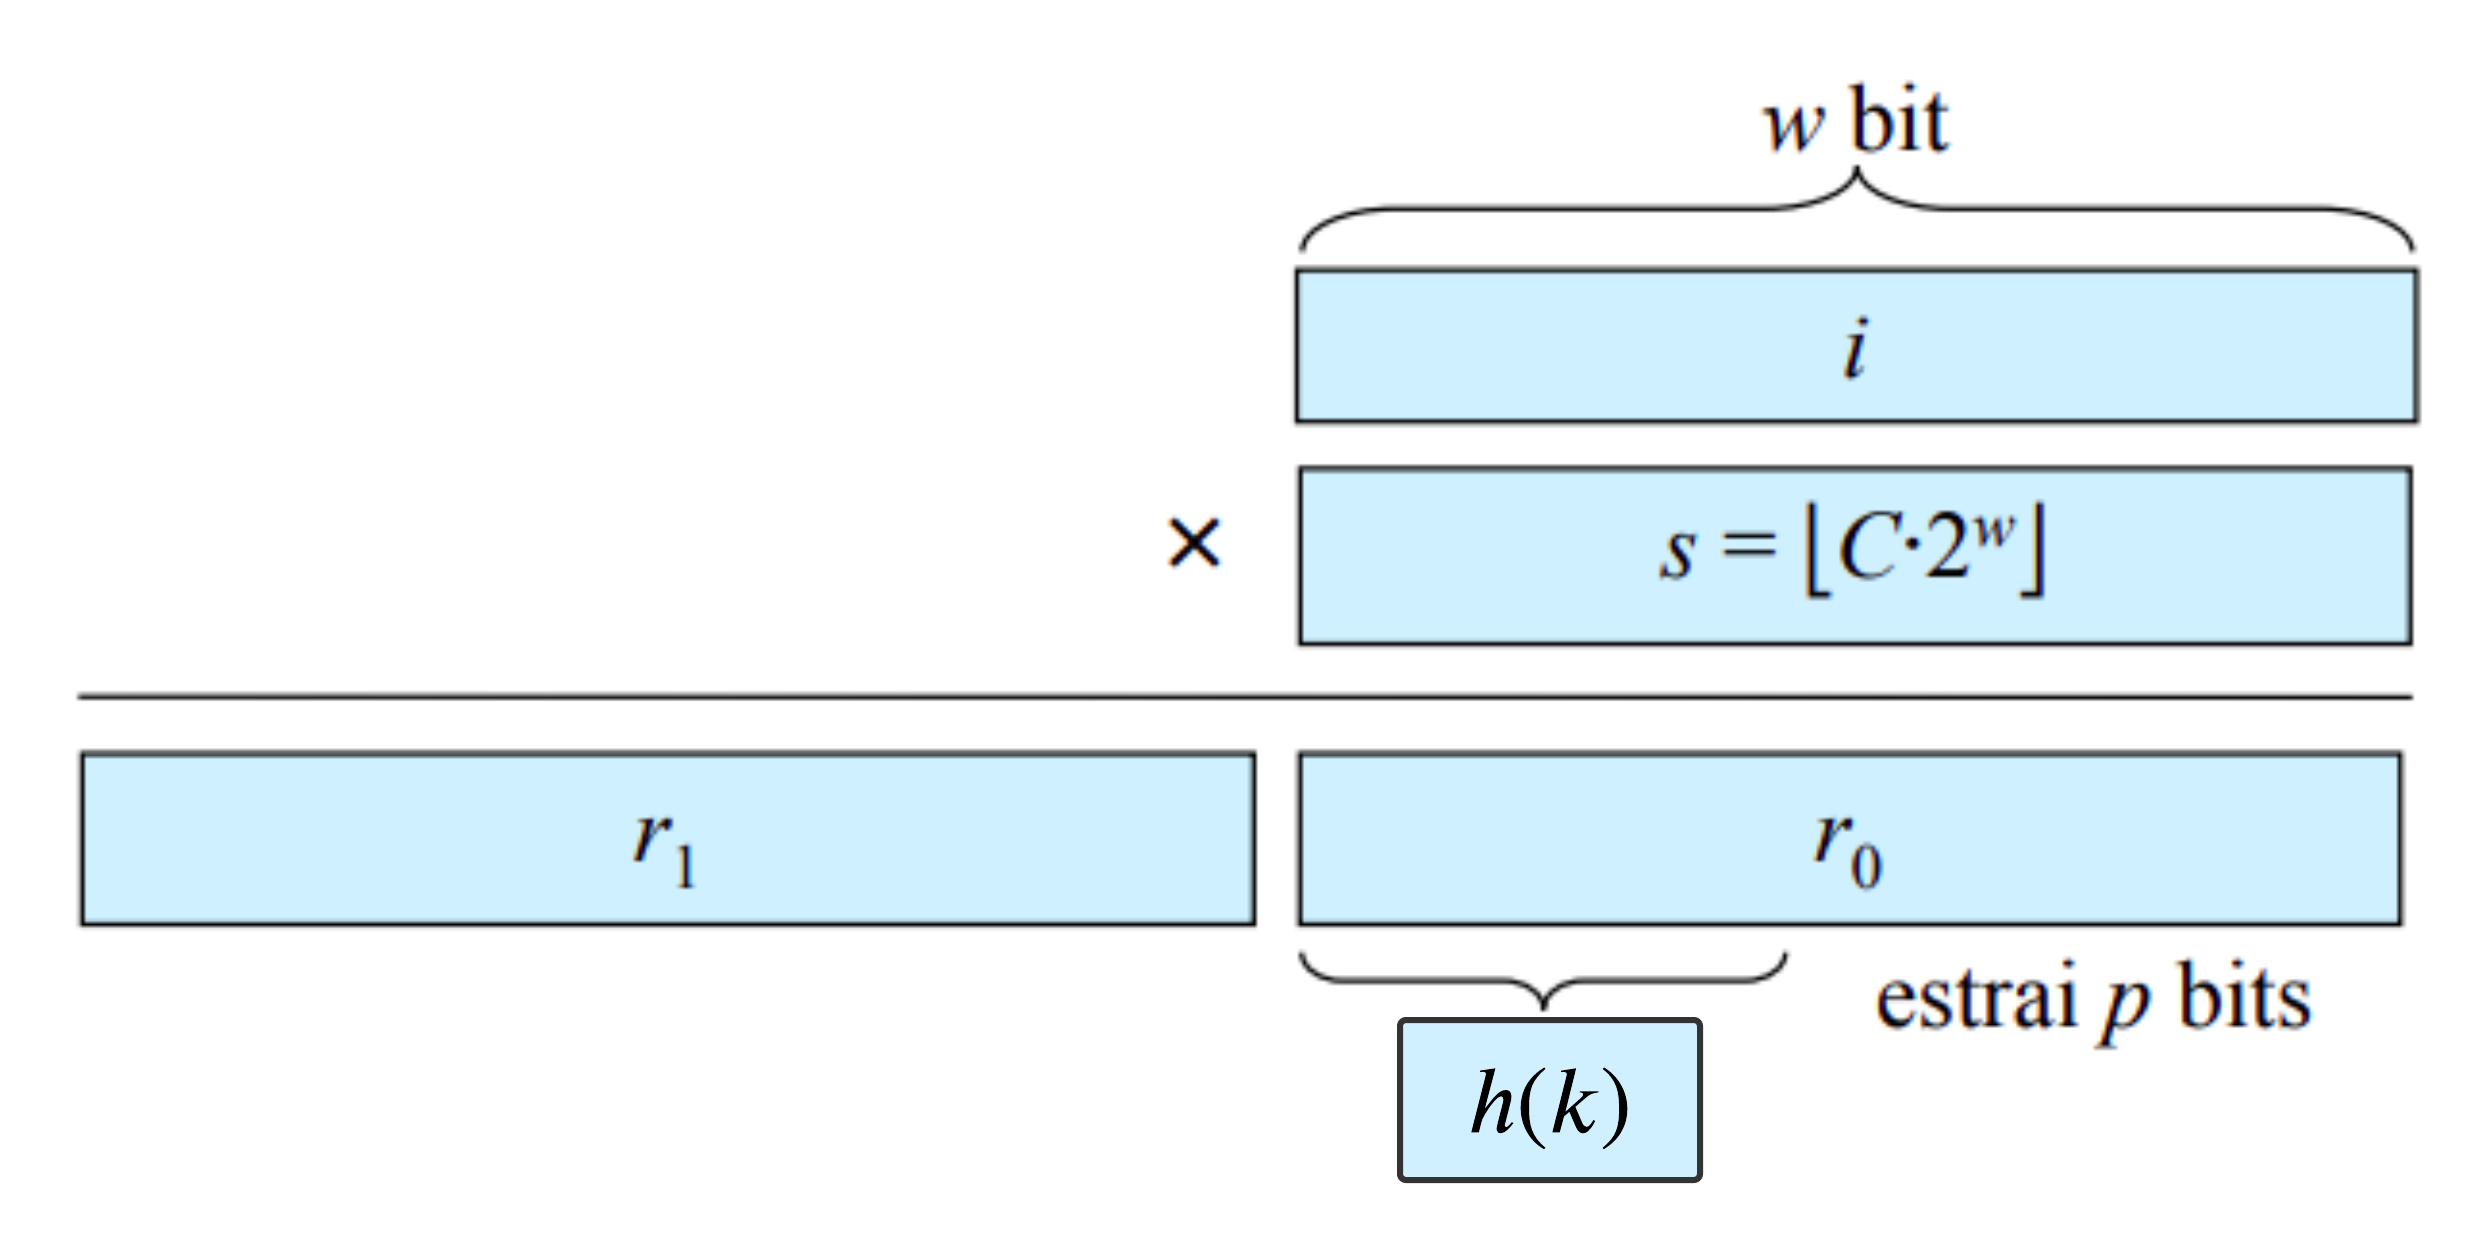
\includegraphics[width=0.8\textwidth]{metodo-moltiplicazione.png}
    \caption{Implementazione efficiente del \emph{metodo della moltiplicazione}}
\end{figure}\noindent
In definitiva, il \emph{metodo della moltiplicazione} sembra offrire una soluzione
sufficientemente efficacie anche se in realtà, la \emph{funzione hash} ottenuta non
gode di \emph{uniformità semplice} e non viene mai usata in applicazioni reali.

\section{Gestione delle collisioni}
Se abbiamo stabilito che non possiamo garantire l'assenza di \emph{collisioni}
dobbiamo definire una metodologia per la loro gestione. In particolare, se,
in fase di inserimento, la posizione in cui dovremmo inserire una chiave è
già occupata, dovremo trovarne una alternativa e, allo stesso modo, se in fase di
ricerca la chiave cercata non è nella posizione attesa, dovremo cercarla
altrove. Questa ricerca dovrebbe costare $O(1)$ nel caso medio e $O(n)$ nel caso
pessimo.

Le tecniche possibili sono due: \emph{liste di trabocco} e \emph{indirizzamento
aperto}. Queste due sono anche chiamate rispettivamente tecniche a
\emph{memorizzazione esterna} e \emph{interna}.

\subsection{Liste di trabocco}
Questa metodologia prevede che tutte le chiavi con lo stesso \emph{hash}
vengano memorizzate in una \emph{lista monodirezionale} o in un \emph{vettore
dinamico}. Ogni cella della \emph{tabella hash} poi conterrà un puntatore alla
testa della \emph{lista} o al primo elemento del \emph{vettore} associato a quella
posizione.

\begin{figure}[h!]
    \centering
    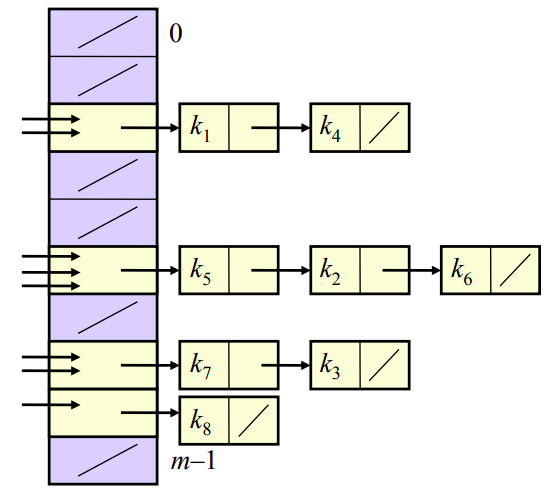
\includegraphics[width=0.6\textwidth]{liste-di-trabocco1.png}
    \caption{Struttura di una \emph{tabella hash} con \emph{liste di trabocco}}
\end{figure}\noindent
La funzione \texttt{insert()} va ad aggiungere in testa la chiave, mentre la
\texttt{lookup()} e la \texttt{remove()} scansionano la \emph{lista} fino
a trovare la chiave cercata.

\paragraph{Complessità}
Per studiare la \emph{complessità} di questa soluzione abbiamo bisogno di
definire alcuni parametri:
\begin{itemize}
    \item $n$: numero di chiavi memorizzate nella \emph{tabella hash};
    \item $m$: dimensione della \emph{tabella hash};
    \item $\alpha=\frac{n}{m}$: \emph{fattore di carico} della \emph{tabella hash};
    \item $I(\alpha)$: numero medio di accessi per la ricerca di una chiave che
    non è presente nella \emph{tabella hash} (ricerca con insuccesso);
    \item $S(\alpha)$: numero medio di accessi per la ricerca di una chiave che
    è presente nella \emph{tabella hash} (ricerca con successo);
\end{itemize}\noindent
Ovviamente il caso pessimo è quello in cui $m=1$ e quindi tutte le chiavi sono
inserite in un'unica lista e quindi la \emph{complessità} è pari a quella che
si avrebbe in un \emph{dizionario} implementato come \emph{vettore non ordinato} o
come \emph{lista}.

\bigskip\noindent
Studiare il caso medio invece, ci richiede di fare delle assunzioni. In particolare,
ipotizziamo che la \emph{funzione hash} costi $\Theta(1)$ e che consenta un
\emph{hashing uniforme}. Fatte queste ipotesi, ci aspettiamo che ogni
\emph{lista}/\emph{vettore} abbia una lunghezza pari ad $\alpha=\frac{n}{m}$.

In una ricerca con insuccesso devono ovviamente essere toccati tutti i valori di
una lista, mentre nelle ricerche con successo, in media, ne vengono toccati la
metà. Questo, unito al fatto che calcolare la posizione di ricerca costa
$\Theta(1)$, ci porta ad avere, rispettivamente, un costo $\Theta(1)+\alpha$ e
$\Theta(1)+\frac{\alpha}{2}$ per le ricerche con insuccesso e con successo.

\bigskip\noindent
Ma qual è il significato del \emph{fattore di carico}?

Il parametro influenza il costo delle operazioni sulla \emph{tabella hash}.
Per esempio, se $n=O(m)$, $\alpha=O(1)$ e quindi tutte le operazioni costano $O(1)$.

\subsection{Indirizzamento aperto}
Il problema delle \emph{liste di trabocco} è che ci costringono a
realizzare una \emph{struttura dati} complessa. L'idea alla base delle
implementazioni a \emph{indirizzamento aperto} invece, è di memorizzare tutte le
chiavi nella \emph{tabella stessa} in modo tale che ogni posizione contenga
una chiave, oppure \texttt{nil}.

Quindi, se in fase di inserimento la posizione calcolata è già
occupata, se ne sceglie un'altra. Per la ricerca invece, si parte dalla posizione
prescelta e si visitano tutte le posizioni alternative fino a quando non si
trova la chiave cercata. Per affrontare nel dettaglia questa tecnica implementativa
diamo alcune definizioni:
\begin{definition}[Ispezione]
    Un'ispezione è l'esame di una posizione durante la ricerca.
\end{definition}\noindent
Ovviamente, il numero massimo di ispezioni coincide con la dimensione $m$ della
\emph{tabella hash}. Modifichiamo la definizione di \emph{funzione hash} in modo
da includere il concetto di \emph{ispezione}.
\begin{definition}[Funzione hash per tabelle ad indirizzamento aperto]
    In una tabella hash implementata con la tecnica dell'indirizzamento aperto,
    la funzione hash $H$ è definita come
    \[H:\mathcal{U}\times\overbrace{\{0,\,\dots,\,m-1\}}^{\text{Numero di ispezione}}
    \to\overbrace{\{0,\,\dots,\,m-1\}}^{\text{Posizione nella tabella}}\]
\end{definition}
\begin{definition}[Sequenza di ispezione]
    Una sequenza di ispezione $[H(k,0),\,H(k,1),\,\dots,\,H(k,m-1)]$ è una
    permutazione degli indici $[0,\,\dots,\,m-1]$ corrispondente all'ordine
    in cui vengono visitate le posizioni della tabella.
\end{definition}\noindent
Generalmente non dovrebbe servire visitare tutte le posizioni, ma in ogni caso,
vogliamo evitare di visitarne più volte la stessa.

\begin{figure}[ht]
    \centering
    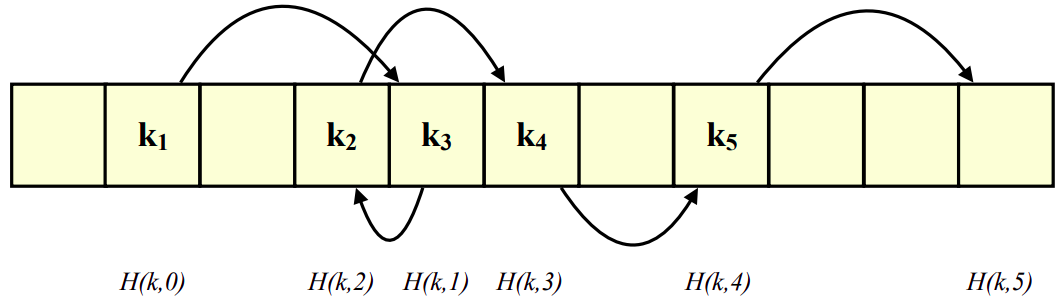
\includegraphics[width=\textwidth]{sequenza-ispezione-1.png}
    \caption{Esempio di \emph{sequenza di ispezione}}
\end{figure}

\newpage\noindent Ma cosa succede al \emph{fattore di carico}?

Siccome $0\leq n\leq m$, anche $\alpha$ è compreso tra 0 e 1 (estremi inclusi).
Questo comporta che la \emph{tabella hash} potrebbe andare in overflow,
ovvero occupare tutte le posizioni.

\bigskip\noindent
Generalizzando il concetto di \emph{uniformità semplice}, diamo la definizione di
\emph{hashing uniforme}.
\begin{definition}[Hashing uniforme]
    Si parla di hashing uniforme quando una chiave ha la stessa probabilità di
    avere come sequenza di ispezione una qualsiasi delle $m!$ permutazioni di
    $[0,\,\dots,\,m-1]$.
\end{definition}\noindent
Nella realtà è difficile raggiungere l'\emph{hashing uniforme}, per cui ci si
accontenta di ottenere alcune delle possibili permutazioni.

Le \emph{sequenze di ispezione} dipendono dalla tecnica di ispezione che si usa e
le più diffuse sono: \emph{ispezione lineare}, \emph{quadratica} e
\emph{doppio hashing}.

\paragraph{Ispezione lineare}
Questa tecnica definisce la \emph{funzione hash} come:
\[H(k,i)=(H_1(k)+h\cdot i)\Mod{m}\]
In questa definizione, $h$ è il passo della sequenza e di conseguenza la
\emph{sequenza di ispezione} per una chiave $k$ diventa:
$[H_1(k),\,H_1(k)+h,\,H_1(k)+2h,\,\dots]$.

Questa tecnica ci permette di avere al massimo $m$ possibili \emph{sequenze} che
sono tutte determinabili dalla posizione della prima \emph{ispezione}. Inoltre,
c'è il problema della cosiddetta \emph{aggregazione primaria} (o \emph{primary
clustering}) che comporta la formazione di sotto sequenze sempre più lunghe di
posizioni occupate, col risultato che una posizione libera preceduta da $i$
posizione occupate viene riempita con probabilità $\frac{i+1}{m}$ e i tempi di
inserimento e cancellazione crescono sempre di più.

\paragraph{Ispezione quadratica}
L'\emph{ispezione quadratica} segue lo stesso principio di quella \emph{lineare},
ma le \emph{ispezioni} hanno un offset che dipende da una funzione quadratica del
numero di \emph{ispezione}. La \emph{funzione hash} è infatti definita come:
\[H(k,i)=(H_1(k)+h\cdot i^2)\Mod{m}\]
Anche in questo caso sono possibili $m$ \emph{sequenze di ispezione}, ma nessuna
di esse è una permutazione e si propone il problema dell'\emph{aggregazione
secondaria} (o \emph{secondary clustering}) ovvero, chiavi con
la stessa posizione iniziale hanno anche \emph{sequenze di ispezione} identiche.

\paragraph{Doppio hashing}
In questo caso $H$ è:
\[H(k,i)=(H_1(k)+i\cdot H_2(k))\Mod{m}\]
dove $H_1(k)$ fornisce la posizione iniziale e $H_2(k)$ l'offset per le
successive \emph{ispezioni}. Sono possibili $m^2$ \emph{sequenze}, ma per
garantire una permutazione completa $H_2(k)$ deve essere coprimo con $H_1(k)$.
Cioè, se $m=2^p$, $H_2(k)$ deve essere un numero dispari, mentre se $m$ è
primo, $H_2(k)$ deve essere un valore minore di $m$.

\begin{minicode}{Implementazione tabella hash con hashing doppio}
\bc{ITEM}[] K\hfill\com{Tabella delle chiavi}
\bc{ITEM}[] V\hfill\com{Tabella dei valori}
\bc{int} m\hfill\com{Dimensione della \emph{tabella hash}}

\nl\ind\bc{HASH} Hash(\bc{int} dim)\\
    \bc{HASH} t = new \bc{HASH}\\
    t.m = dim\\
    t.K = new \bc{ITEM}[dim]\\
    t.V = new \bc{ITEM}[dim]\\
    \indf for (i = 0 to dim - 1) do\\
        t.K[i] = nil\\
    \indf return t

\nl\com{Cerca la posizione associata ad una chiave}
\rmbreak\ind\bc{int} scan(\bc{ITEM} k, \bc{boolean} insert)\\
    \bc{int} delpos = m\hfill\com{Prima posizione deleted}
    \bc{i} = 0\hfill\com{Numero di \emph{ispezione}}
    \bc{j} = H(k)\hfill\com{Posizione di partenza}
    \indf while (K[i] $\neq$ k and K[j] $\neq$ nil and i < m) do\\
        \indff if (K[j] == deleted and delpos == m) then\\
            delpos = j\\
        \indff j = (j + H'(k)) mod m\\
        \indff i = i + 1\\
    \indf if (insert and K[j] $\neq$ k and delpos < m) then\\
        return delpos\\
    \indf return j

\nl\com{Cerca e restituisce il valore associato a una chiave oppure nil}
\rmbreak\ind\bc{ITEM} lookup(\bc{ITEM} k)\\
    \bc{int} i = scan(k, false)\\
    \indf if (k[i] == k) then\\
        return V[i]\\
    \indf else\\
        return nil
\end{minicode}
\newpage
\begin{codecont}
\com{Inserisce un'associazione chiave-valore o ne modifica il valore associato}
\rmbreak\ind insert(\bc{ITEM} k, \bc{ITEM} v)\\
    \bc{int} i = scan(k, true)\\
    if (K[i] == nil or K[i] == deleted or K[i] == k) then\\
        \indf k[i] = k\hfill\com{È inutile se K[i] == k}
        \indf V[i] = v\\
    \ind else\\
        \indf \{ Errore:\,la tabella è piena \}

\nl\com{Rimuove un'associazione chiave-valore}
\rmbreak\ind remove(\bc{ITEM} k)\\
    \ind \bc{int} i = scan(k, false)\\
    \ind if (K[i] == k) then\\
        \indf K[i] = deleted\\
        \indf V[i] = nil\\
\end{codecont}

\bigskip\noindent
Esaminiamo più nel dettaglio la funzione \texttt{scan()}. Può infatti risultare
strano il fatto che abbiamo introdotto il valore \texttt{deleted} che usiamo al
posto di \texttt{nil} per marcare una posizione come libera dopo una cancellazione.
Questo serve a evitare situazioni come quella in figura, in cui la ricerca della
chiave $k_5$ si interrompe all'\emph{ispezione} della posizione \texttt{nil}
facendo erroneamente credere che $k_5$ non sia presente nella \emph{tabella hash}.

\begin{figure}[h!]
    \centering
    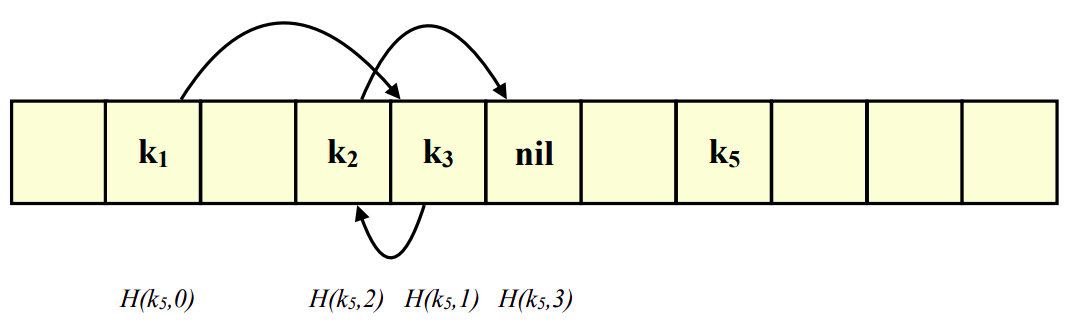
\includegraphics[width=\textwidth]{sequenza-ispezione-2.png}
    \caption{\emph{Sequenza di inspezione} errata}
\end{figure}\noindent
L'utilizzo del valore \texttt{deleted} al posto di \texttt{nil} ci consente di
marcare le posizioni nelle quali in precedenza c'era un valore che poi è stato
eliminato. In particolare, le posizioni \texttt{deleted} sono considerate come
piene in fase di ricerca e vuote in fase di inserimento.

Questa soluzione risolve il problema della ricerca, ma rende il tempo di ricerca
non più dipendente dal \emph{fattore di carico} $\alpha$ e fa sì che il
concatenamento sia più comune nelle implementazioni che ammettono la rimozione.

\newpage
\subsection{Complessità delle diverse implementazioni}
Mettiamo a confronto le \emph{complessità} di alcune delle implementazioni viste:
\begin{table}[ht]
    \renewcommand{\arraystretch}{1.5}
    \centering
    \begin{tabular}{|l|c|c|c|}
        \hline
        \textbf{Tecnica} & \bm{$\alpha$} & \bm{$I(\alpha)$} & \bm{$S(\alpha)$}\\
        \hline
        Lineare & $0\leq\alpha<1$ & $\frac{(1-\alpha)^2+1}{2(1-\alpha)^2}$ &
        $\frac{1-\frac{\alpha}{2}}{1-\alpha}$\\
        \hline
        Hashing doppio & $0\leq\alpha<1$ & $\frac{1}{1-\alpha}$ &
        $-\frac{1}{\alpha}\ln(1-\alpha)$\\
        \hline
        Liste di trabocco & $\alpha\geq0$ & $1+\alpha$ & $1+\frac{\alpha}{2}$\\
        \hline
    \end{tabular}
\end{table}
\begin{figure}[ht!]
    \centering
    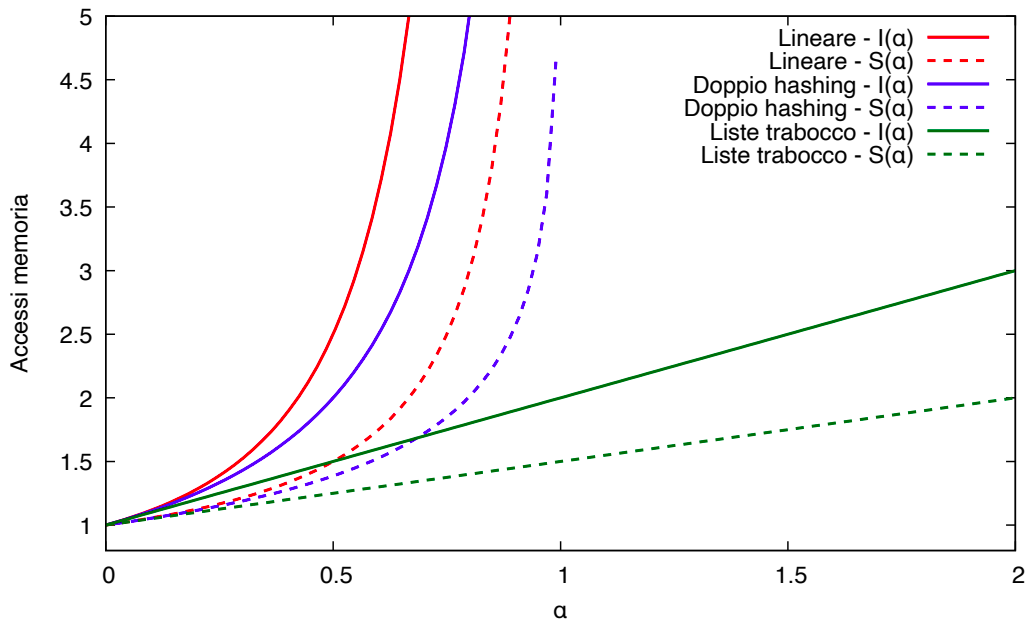
\includegraphics[width=\textwidth]{complessita-hash-table.png}
    \caption{\emph{Complessità} delle \emph{tabelle hash} a confronto}
\end{figure}

\paragraph{Conclusioni}
Per concludere possiamo dire che le \emph{tabelle hash} permettono di implementare
in modo molto efficiente dei \emph{dizionari}, ma hanno una scarsa \q{locality
of reference} che genera molte \emph{cache miss} e inoltre, non permettono di
ordinare le chiavi.
\chapter{Analisi ammortizzata}
Dopo aver parlato a lungo di \emph{strutture dati}, vediamo ora una tecnica che
ci permette di effettuare una stima dall'alto del costo che è necessario pagare
per eseguire delle operazioni su quelle strutture.
\begin{definition}[Analisi ammortizzata]
    L'analisi ammortizzata è una tecnica per l'analisi di complessità che valuta
    il tempo richiesto per eseguire, nel caso pessimo, una sequenza di operazioni
    su una struttura dati.
\end{definition}\noindent
In generale, esistono operazioni più o meno costose, ma se le operazioni più
costose sono poco frequenti, il loro costo può essere ammortizzato da quelle
meno costose.

È importante esplicitare la profonda differenza tra l'analisi del caso medio
e l'\emph{analisi ammortizzata}, effettuata sul caso pessimo. Nella prima,
l'analisi è di tipo probabilistico ed è effettuata sulle singole operazioni,
mentre, la seconda, è un'analisi deterministica effettuata su una sequenza di
operazioni, e in particolare, sulla sequenza più costosa possibile.

\section{Metodi per l'analisi ammortizzata}
Esistono diverse tecniche per realizzare un'\emph{analisi ammortizzata}.

\begin{definition}[Metodo dell'aggregazione]
    Col metodo dell'aggregazione si calcola la complessità $T(n)$ necessaria
    per eseguire $n$ operazioni in sequenza nel caso pessimo, quindi, si calcola
    il costo ammortizzato come $T(n)/n$ cioè come media su $n$ operazioni.
\end{definition}

\noindent
Definiamo meglio i termini presenti nella definizione:
\begin{itemize}
    \item \emph{Sequenza}: è una sequenza di operazioni che permettono alla
    \emph{struttura dati} di evolvere;
    \item \emph{Caso pessimo}: è la \emph{sequenza} con \emph{complessità} più
    alta tra tutte quelle possibili;
    \item \emph{Aggregazione}: la \emph{complessità} $T(n)$ è ottenuta mediante
    una sommatoria dei costi delle singole operazioni;
\end{itemize}

\newpage
\begin{definition}[Metodo degli accantonamenti]
    Col metodo degli accantonamenti si assegna ad ogni operazione un costo
    ammortizzato che può anche essere diverso dal costo effettivo. In particolare,
    le operazioni meno costose vengono caricate di un costo aggiuntivo detto
    credito, che viene poi usato per pagare le operazioni più costose.
\end{definition}
\begin{note}
    Potenzialmente, ad ogni operazione potrebbe essere assegnato un costo diverso.
\end{note}

\noindent
In generale, utilizzando il \emph{metodo degli accantonamenti}, il \emph{costo
ammortizzato} assegnato alle operazioni meno costose è definito come:
\[\emph{Costo ammortizzato}=\emph{Costo effettivo}+\emph{Credito prodotto}\]
Viceversa, il costo per le operazioni più costose è:
\[\emph{Costo ammortizzato}=\emph{Costo effettivo}-\emph{Credito consumato}\]
Quindi, l'obiettivo, quando si utilizza questo metodo, è dimostrare che la somma
dei \emph{costi ammortizzati} $a_i$ è un limite superiore ai costi effettivi
$c_i$, ovvero che vale:
\[\sum_{i=1}^nc_i\leq\sum_{i=1}^na_i\]
Ovviamente, la dimostrazione deve valere per tutte le sequenze, ma se vale per il
caso pessimo vale anche per tutti gli altri. Il \emph{credito} dopo la $t$-esima
operazione è sempre positivo ed è espresso dalla seguente formula:
\[\sum_{i=1}^ta_i-\sum_{i=1}^tc_i\geq0\]

\begin{definition}[Metodo del potenziale]
    Col metodo del potenziale si associa una funzione di potenziale $\Phi$ ad
    uno stato $S$ della struttura. La funzione $\Phi$ definisce la \q{quantità
    di lavoro} $\Phi(S)$ che è stato contabilizzata nell'analisi ammortizzata,
    ma non ancora spesa.
\end{definition}
\begin{note}
    $\Phi(S)$ rappresenta la quantità di energia potenziale che è stata
    \q{immagazzinata} in quello stato e che può essere spesa per eseguire le
    operazioni più costose.
\end{note}\noindent
In pratica, $\Phi(S)$ può essere vista come la cumulazione dei \emph{crediti
prodotti} dalle operazioni fino al raggiungimento dello stato $S$.

\bigskip\noindent
In generale, il \emph{costo ammortizzato} di un'operazione è pari a:
\[\begin{array}[t]{rcl}
    \emph{Costo ammortizzato} & = & \emph{Costo effettivo}+\emph{Variazione di potenziale}\\
    a_i & = & c_i + (\Phi(S_i)-\Phi(S_{i-1}))
\end{array}\]
dove $S_i$ è lo stato associato all'$i$-esima operazione.
Se proviamo a calcolare il \emph{costo ammortizzato} di una sequenza di $n$
operazioni, vale quanto segue:
\[A\begin{array}[t]{cl}
    = & \sum_{i=1}^na_i\\
    = & \sum_{i=1}^n\left(c_i+\Phi(S_i)-\Phi(S_{i-1})\right)\\
    = & \sum_{i=1}^nc_i+\sum_{i=1}^n\left(\Phi(S_i)-\Phi(S_{i-1})\right)\\
    = & C + \left(\Phi(S_1) - \Phi(S_{0})\right) + \left(\Phi(S_2) - \Phi(S_1)\right)+\dots+\left(\Phi(S_n)-\Phi(S_{n-1})\right)\\
    = & C + \Phi(S_n) - \Phi(S_0)
\end{array}\]
Allora, se $\Phi(S_n)-\Phi(S_0)\geq0$, $A$ è un limite superiore al costo effettivo.

\section{Esempio di analisi ammortizzata}
\begin{eg}[Contatore binario]
Si consideri un contatore binario a $k$ bit implementato come un vettore $A$ di
booleani, nel quale $A[0]$ è il bit meno significativo e $A[k-1]$ il più significativo.
Il valore del contatore corrisponde al risultato della seguente sommatoria:
\[x=\sum_{i=0}^{k-1}A[i]\cdot2^i\]
Alla struttura del contatore è associata soltanto la funzione \texttt{increment}
per l'incremento del valore.

\begin{minicode}{Implementazione funzione increment per contatori binari}
\ind increment(\bc{int}[] A, int k)\\
    \bc{int} i = 0\\
    \indf while (i < k and A[i] == 1) do\hfill\com{Imposta a 0 la prima sequenza di bit a 1}
        A[i] = 0\\
        i = i + 1\\
    \indf if (i < k) then\hfill\com{Se $i < k$ non c'è overflow}
        A[i] = 1
\end{minicode}\noindent
Se $k=8$, si ottiene un contatore binario a 8 bit e la seguente tabella ne mostra
lo stato dopo il sedicesimo incremento.
\begin{table}[h!]
    \centering
    \renewcommand{\arraystretch}{1.2}
    \begin{tabular}{|c|c|c|c|c|c|c|c|c|}
        \hline
        \bm{$x$} & \bm{$A[7]$} & \bm{$A[6]$} & \bm{$A[5]$} & \bm{$A[4]$} &
        \bm{$A[3]$} & \bm{$A[2]$} & \bm{$A[1]$} & \bm{$A[0]$}\\
        \hline
        0 & 0 & 0 & 0 & 0 & 0 & 0 & 0 & 0\\
        \hline
        1 & 0 & 0 & 0 & 0 & 0 & 0 & 0 & 1\\
        \hline
        2 & 0 & 0 & 0 & 0 & 0 & 0 & 1 & 0\\
        \hline
        3 & 0 & 0 & 0 & 0 & 0 & 0 & 1 & 1\\
        \hline
        4 & 0 & 0 & 0 & 0 & 0 & 1 & 0 & 0\\
        \hline
        5 & 0 & 0 & 0 & 0 & 0 & 1 & 0 & 1\\
        \hline
        6 & 0 & 0 & 0 & 0 & 0 & 1 & 1 & 0\\
        \hline
        7 & 0 & 0 & 0 & 0 & 0 & 1 & 1 & 1\\
        \hline
        8 & 0 & 0 & 0 & 0 & 1 & 0 & 0 & 0\\
        \hline
        9 & 0 & 0 & 0 & 0 & 1 & 0 & 0 & 1\\
        \hline
        10 & 0 & 0 & 0 & 0 & 1 & 0 & 1 & 0\\
        \hline
        11 & 0 & 0 & 0 & 0 & 1 & 0 & 1 & 1\\
        \hline
        12 & 0 & 0 & 0 & 0 & 1 & 1 & 0 & 0\\
        \hline
        13 & 0 & 0 & 0 & 0 & 1 & 1 & 0 & 1\\
        \hline
        14 & 0 & 0 & 0 & 0 & 1 & 1 & 1 & 0\\
        \hline
        15 & 0 & 0 & 0 & 0 & 1 & 1 & 1 & 1\\
        \hline
        16 & 0 & 0 & 0 & 1 & 0 & 0 & 0 & 0\\
        \hline
    \end{tabular}
\end{table}

\bigskip\noindent
Proviamo ora a realizzare una stima dall'alto del costo della funzione
\texttt{increment} usando i metodi per l'analisi ammortizzata.

\paragraph{Metodo dell'aggregazione}
Utilizzando questo metodo ci chiediamo quale sia il costo $T(n)$ da pagare per
eseguire $n$ operazioni in sequenza.

Inizialmente potremmo notare che per rappresentare $n$ in binario servono
$k=\lceil\log(n+1)\rceil$ bit. Un'invocazione di \texttt{increment} nel caso
pessimo richiede un tempo $O(k)$, quindi $n$ invocazioni costano $T(n)=O(nk)$.
A questo punto, il costo ammortizzato di ogni operazione è $T(n)/n=O(nk)/n=O(k)=O(\log n)$.

Se però notiamo che il costo per eseguire l'intera sequenza è proporzionale al
numero di bit che vengono modificati, possiamo provare a realizzare una stima
più ristretta. Proviamo quindi a contare per ogni riga e per ogni colonna il
numero di bit che sono stati modificati.

\begin{table}[h!]
    \centering
    \renewcommand{\arraystretch}{1.2}
    \begin{tabular}{|c|c|c|c|c|c|c|c|c|c|}
        \hline
        \bm{$x$} & \bm{$A[7]$} & \bm{$A[6]$} & \bm{$A[5]$} & \bm{$A[4]$} &
        \bm{$A[3]$} & \bm{$A[2]$} & \bm{$A[1]$} & \bm{$A[0]$} & \bm{$\#bit$}\\
        \hline
        0 & 0 & 0 & 0 & 0 & 0 & 0 & 0 & 0 & 0\\
        \hline
        1 & 0 & 0 & 0 & 0 & 0 & 0 & 0 & \color{red}{1} & 1\\
        \hline
        2 & 0 & 0 & 0 & 0 & 0 & 0 & \color{red}{1} & \color{red}{0} & 2\\
        \hline
        3 & 0 & 0 & 0 & 0 & 0 & 0 & 1 & \color{red}{1} & 1\\
        \hline
        4 & 0 & 0 & 0 & 0 & 0 & \color{red}{1} & \color{red}{0} & \color{red}{0} & 3\\
        \hline
        5 & 0 & 0 & 0 & 0 & 0 & 1 & 0 & \color{red}{1} & 1\\
        \hline
        6 & 0 & 0 & 0 & 0 & 0 & 1 & \color{red}{1} & \color{red}{0} & 2\\
        \hline
        7 & 0 & 0 & 0 & 0 & 0 & 1 & 1 & \color{red}{1} & 1\\
        \hline
        8 & 0 & 0 & 0 & 0 & \color{red}{1} & \color{red}{0} & \color{red}{0} & \color{red}{0} & 4\\
        \hline
        9 & 0 & 0 & 0 & 0 & 1 & 0 & 0 & \color{red}{1} & 1\\
        \hline
        10 & 0 & 0 & 0 & 0 & 1 & 0 & \color{red}{1} & \color{red}{0} & 2\\
        \hline
        11 & 0 & 0 & 0 & 0 & 1 & 0 & 1 & \color{red}{1} & 1\\
        \hline
        12 & 0 & 0 & 0 & 0 & 1 & \color{red}{1} & \color{red}{0} & \color{red}{0} & 3\\
        \hline
        13 & 0 & 0 & 0 & 0 & 1 & 1 & 0 & \color{red}{1} & 1\\
        \hline
        14 & 0 & 0 & 0 & 0 & 1 & 1 & \color{red}{1} & \color{red}{0} & 2\\
        \hline
        15 & 0 & 0 & 0 & 0 & 1 & 1 & 1 & \color{red}{1} & 1\\
        \hline
        16 & 0 & 0 & 0 & \color{red}{1} & \color{red}{0} & \color{red}{0} & \color{red}{0} & \color{red}{0} & 5\\
        \hline
        \#bit & 0 & 0 & 0 & 1 & 2 & 4 & 8 & 16 &\\
        \hline
    \end{tabular}
\end{table}\noindent
Guardando l'ultima riga possiamo notare che il bit in posizione $A[0]$ viene
modificato ad ogni incremento, quello in $A[1]$ ogni due, quello in $A[2]$ ogni
4 e così via. Di conseguenza, il costo $T(n)$ è una funzione di questo tipo:
\[T(n)=\sum_{i=0}^{k-1}\left\lfloor\frac{n}{2^i}\right\rfloor\leq n\sum_{i=0}^{k-1}\frac
{1}{2^i}\leq n\sum_{i=0}^{+\infty}\left(\frac{1}{2}\right)^i=2n\]
e quindi il costo ammortizzato vale:
\[\frac{T(n)}{n}\leq\frac{2n}{n}=2=O(1)\]

\paragraph{Metodo degli accantonamenti}
Supponiamo che il costo effettivo della \texttt{increment} sia $d$, dove $d$ è
il numero di bit che vengono modificati ad ogni incremento. Proviamo però ad
assegnare alla \texttt{increment} un costo di $2$ che include 1 per il costo
effettivo che si paga per cambiare un bit da 0 a 1 e 1 per il futuro cambio
dello stesso bit da 1 a 0.

Di conseguenza, in ogni istante, il credito è pari al numero di bit a 1
presenti e quindi il costo totale vale $O(n)$ e il costo ammortizzato $O(1)$.

\paragraph{Metodo del potenziale}
Scegliamo come funzione di potenziale $\Phi$ il numero di bit a 1 presenti nel
contatore. Ad ogni utilizzo della funzione \texttt{increment}, se $t$ è il numero
di bit a 1 incontrati prima del primo 0, il costo effettivo è $1+t$ perché
cambiamo lo stato di tutti i primi $t$ bit a 1 e del primo bit a 0.

La variazione di potenziale, invece, vale $1-t$ in quanto tutti i bit a 1
incontrati diventano 0 e il primo bit a 0 diventa 1. Quindi, se allo stato $S_i$
$\Phi(S_i)=t$, allo stato $S_{i+1}$ $\Phi(S_{i+1})=1$ e, conseguentemente, la
variazione di potenziale tra lo stato $S_{i+1}$ e lo stato $S_i$ vale:
\[\Phi(S_{i+1})-\Phi(S_i)=1-t\]
Il costo ammortizzato di un'invocazione della \texttt{increment}, allora, vale:
\[\emph{Costo ammortizzato}\begin{array}[t]{cl}
    = & \emph{Costo effettivo}+\emph{Variazione di potenziale}\\
    = & (1+t)+(1-t)\\
    = & 2 = O(1)
\end{array}\]
Inoltre, poiché allo stato $S_0$, $\Phi(S_0)=0$ perché non ci sono bit impostati a
1, e allo stato $S_n$, $\Phi(S_n)\geq0$, risulta verificata anche la
condizione $\Phi(S_n)-\Phi(S_0)\geq0$.
\end{eg}

\section{Vettori dinamici}
Possiamo utilizzare le tecniche di \emph{analisi ammortizzata} per stimare la
\emph{complessità} delle operazioni di inserimento e cancellazione nei vettori
con ridimensionamento dinamico della dimensione.

Prima però vediamo brevemente cosa significa \q{ridimensionamento dinamico della
dimensione}. Quando si implementa una \emph{\hyperref[def:27]{sequenza}}
utilizzando un vettore, se ne specifica una dimensione iniziale detta
\emph{capacità}. Ovviamente, non è sempre nota a priori la quantità di elementi
che dovranno essere inseriti nella struttura, e quindi la \emph{capacità} iniziale
può rivelarsi insufficiente. I \emph{vettori dinamici} risolvono questo problema
allocando un nuovo vettore con una capacità maggiore e ricopiando in esso tutti
i valori presenti nel vettore originale, che poi può essere eliminato.

\subsection{Inserimento}
Quando in fase di inserimento si rende necessario aumentare la dimensione del
vettore, esistono due principali metodologie di approccio: \emph{incremento fisso}
e \emph{incremento variabile}.

Il primo approccio prevede che la \emph{capacità} venga incrementata di un fattore
fisso (e.g. $+1$, $+2$, $+10$, \dots), mentre il secondo è dipendente dalla dimensione
attuale della struttura (e.g. $\cdot2$, $\cdot1.5$, \dots).

Ma qual è il metodo migliore? Proviamo a utilizzare l'\emph{analisi ammortizzata}
per realizzare una stima.

\paragraph{Incremento fisso}
Il costo effettivo di un inserimento con ridimensionamento fisso è descritto
dalla seguente espressione:
\[c_i=\begin{cases}
    i & \text{se}\ (i\Mod{d}) = 1\footnotemark\\
    1 & \text{altrimenti}
\end{cases}\]
dove $d$ è sia la dimensione iniziale che il valore di cui viene incrementata.
\footnotetext{L'inserimento ha un costo $i$ quando $(i\Mod{d})=1$ perché se è stata
raggiunta la dimensione massima quell'operazione di modulo vale 1}

\newpage\noindent
Supponiamo $d=4$ e vediamo il costo delle prime 17 operazioni di inserimento:
\begin{table}[ht]
    \renewcommand{\arraystretch}{1.2}
    \centering
    \begin{tabular}{|c|l|}
        \hline
        \bm{$n$} & \textbf{Costo}\\
        \hline
        1 & 1\\
        \hline
        2 & 1\\
        \hline
        3 & 1\\
        \hline
        4 & 1\\
        \hline
        5 & $1+d=5$\\
        \hline
        6 & 1\\
        \hline
        7 & 1\\
        \hline
        8 & 1\\
        \hline
        9 & $1+2d=9$\\
        \hline
        10 & 1\\
        \hline
        11 & 1\\
        \hline
        12 & 1\\
        \hline
        13 & $1+3d=13$\\
        \hline
        14 & 1\\
        \hline
        15 & 1\\
        \hline
        16 & 1\\
        \hline
        17 & $1+4d=17$\\
        \hline
    \end{tabular}
\end{table}

\noindent A questo punto, calcoliamo il costo effettivo di $n$ operazioni:
\[\renewcommand{\arraystretch}{1.3}
    T(n)\begin{array}[t]{cll}
    = & \sum_{i=1}^nc_i\\
    = & n + \sum_{j=1}^{\lfloor n/d\rfloor}d\cdot j\\
    = & n + d\sum_{j=1}^{\lfloor n/d\rfloor}j\\
    = & n + d\frac{\left(\lfloor n/d\rfloor+1\right)\lfloor n/d\rfloor}{2}\\
    \leq & n + \frac{\left(n/d+1\right)n}{2} & \quad\emph{Rimozione dell'intero inferiore}\\
    = & n + \frac{n^2/d+n}{2}=O(n^2)
\end{array}\]
Il \emph{costo ammortizzato} vale:
\[\frac{T(n)}{n}=\frac{O(n^2)}{n}=O(n)\]

\paragraph{Incremento dinamico}
Supponendo che ad ogni incremento la dimensione del vettore venga raddoppiata, il
costo effettivo vale:
\[c_i=\begin{cases}
    i & \text{se}\ \exists k\in\mathbb{Z}^+_0:i=2^k+1\\
    1 & \text{altrimenti}
\end{cases}\]
\newpage\noindent
Se la dimensione iniziale è 1, il costo delle prime 17 operazioni è il seguente:
\begin{table}[h!]
    \renewcommand{\arraystretch}{1.2}
    \centering
    \begin{tabular}{|c|l|}
        \hline
        \bm{$n$} & \textbf{Costo}\\
        \hline
        1 & 1\\
        \hline
        2 & $1+2^0=2$\\
        \hline
        3 & $1+2^1=3$\\
        \hline
        4 & 1\\
        \hline
        5 & $1+2^2=5$\\
        \hline
        6 & 1\\
        \hline
        7 & 1\\
        \hline
        8 & 1\\
        \hline
        9 & $1+2^3=9$\\
        \hline
        10 & 1\\
        \hline
        11 & 1\\
        \hline
        12 & 1\\
        \hline
        13 & 1\\
        \hline
        14 & 1\\
        \hline
        15 & 1\\
        \hline
        16 & 1\\
        \hline
        17 & $1+2^4=17$\\
        \hline
    \end{tabular}
\end{table}

\noindent Il costo effettivo di $n$ operazioni vale:
\[\renewcommand{\arraystretch}{1.3}
    T(n)\begin{array}[t]{cll}
    = & \sum_{i=1}^nc_i\\
    = & n + \sum_{j=0}^{\lfloor\log n\rfloor}2^j\\
    = & n + 2^{\lfloor\log n\rfloor+1}-1\\
    \leq & 2^{\log(n)+1}-1 & \quad\emph{Rimozione dell'intero inferiore}\\
    = & n+2n-1=O(n)
\end{array}\]
e di conseguenza quello \emph{ammortizzato} è:
\[\frac{T(n)}{n}=\frac{O(n)}{n}=O(1)\]
Giunti a questo punto, siamo riusciti a dimostrare che l'incremento dinamico
ha un costo inferiore all'incremento fisso.

\subsection{Cancellazione}
Se il vettore non è ordinato, rimuovere un elemento significa spostare l'ultimo
elemento della \emph{sequenza} nella posizione dell'elemento da rimuovere.

Per ridurre lo spreco di memoria, è opportuno ridurre la dimensione del vettore
quando il \emph{fattore di carico} $\alpha=\frac{\emph{Dim}}
{\emph{Capacità}}$\footnotemark\ scende sotto una certa soglia.
\footnotetext{Il valore \emph{Dim} rappresenta il numero di elementi che
in dato momento sono presenti nella struttura}

L'operazione di riduzione della \emph{capacità} è detta \emph{contrazione} e,
similmente a quanto avviene con l'\emph{espansione}, prevede che venga allocato un nuovo
vettore di dimensione inferiore a quella attuale, che vi vengano copiati i
valori del vettore originale e che quindi quest'ultimo venga eliminato.

\bigskip\noindent
Ma qual è la soglia di \emph{contrazione} ottimale?

Una prima strategia potrebbe essere quella di dimezzare la \emph{capacità} quando
\emph{Dim} raggiunge la metà della \emph{capacità}, cioè quando $\alpha=
\frac{1}{2}$. Il problema di questa scelta è che dopo la \emph{contrazione}
nella struttura non rimangono posizioni libere e quindi un successivo inserimento
richiederebbe di fare subito un'\emph{espansione}.

Una strategia migliore è quella invece di scegliere $\alpha=\frac{1}{4}$. In
questo modo, se quando viene raggiunta la \emph{soglia di contrazione}, si va
a dimezzare la \emph{capacità}, il \emph{fattore di carico} $\alpha$, invece di
aumentare fino a $1$ si fermerà a $\frac{1}{2}$ concedendoci di aggiungere al
vettore tanti elementi quanti sono quelli già presenti prima di dover effettuare
un'\emph{espansione}.

\paragraph{Analisi del costo}
Proviamo a stimare il costo di questa seconda soluzione utilizzando il
\emph{metodo del potenziale}. Scegliamo una funzione di potenziale $\Phi$ che
vale 0 all'inizio e immediatamente dopo un'\emph{espansione} o una
\emph{contrazione} e il cui valore cresca fino a raggiungere il numero di
elementi presenti nella struttura quando $\alpha=1$ e diminuisca fino a un
quarto quando $\alpha$ si riduce alla \emph{soglia di contrazione}.

Quindi, la definizione di $\Phi$ è la seguente:
\[\Phi=\begin{cases}
    2\cdot\emph{Dim}-\emph{Capacità} & \text{se}\ \alpha\geq\frac{1}{2}\\
    \frac{\emph{Capacità}}{2}-\emph{Dim} & \text{se}\ \alpha<\frac{1}{2}
\end{cases}\]
Vediamone il valore in alcuni casi particolari:
\begin{itemize}
    \item $\alpha=\frac{1}{2}$: è stata appena effettuata un'\emph{espansione} o
    una \emph{contrazione} e quindi $\Phi=0$;
    \item $\alpha=1$ la struttura è piena, ovvero $\emph{Dim}=\emph{Capacità}$
    e quindi $\Phi=\emph{Dim}=\emph{Capacità}$;
    \item $\alpha=\frac{1}{4}$: il \emph{fattore di carico} ha raggiunto la
    \emph{soglia di contrazione}, ovvero $\emph{Dim}=\frac{\emph{Capacità}}
    {4}$ e quindi $\Phi=\emph{Dim}$;
\end{itemize}
Una funzione di potenziale di questo tipo ci garantisce che il potenziale presente
nel momento in cui si effettua un'\emph{espansione} o una \emph{contrazione} sia
sufficiente per \q{pagare} quelle stesse operazioni.

Proviamo quindi a calcolare il \emph{costo ammortizzato} in base ai diversi valori
di $\alpha$:
\begin{itemize}
    \item $\alpha\geq\frac{1}{2}$:
    \[a_i\begin{array}[t]{cl}
        = & c_i + \Phi_i - \Phi_{i-1}\\
        = & 1 + (2\emph{Dim}_i - \emph{Capacità}_i) - (2\emph{Dim}_{i-1}-\emph{Capacità}_{i-1})\\
        = & 1 + 2(\emph{Dim}_{i-1}+1) - \emph{Capacità}_i - 2\emph{Dim}_{i-1}+\emph{Capacità}_{i-1}\\
        = & 1 + 2(\emph{Dim}_{i-1}+1) - \emph{Capacità}_{i-1} - 2\emph{Dim}_{i-1}+\emph{Capacità}_{i-1}\\
        = & 1 + 2\emph{Dim}_{i-1}+2 - \emph{Capacità}_{i-1} - 2\emph{Dim}_{i-1}+\emph{Capacità}_{i-1}\\
        = & 3
    \end{array}\]
    \item $\alpha=1$:
    \[a_i\begin{array}[t]{cl}
        = & c_i+\Phi_i-\Phi_{i-1}\\
        = & 1 + \emph{Dim}_{i-i}+(2\emph{Dim}_i+\emph{Capacità}_i)-(2\emph{Dim}_{i-1}-\emph{Capacità}_{i-1})\\
        = & 1 + \emph{Dim}_{i-i}+2(\emph{Dim}_{i-1}+1)-2\emph{Dim}_{i-1}-2\emph{Dim}_{i-1}+\emph{Dim}_{i-1}\\
        = & 3
    \end{array}\]
\end{itemize}
In entrambi i casi il costo è $O(1)$.

\begin{note}
    Poiché non è conveniente che il \emph{fattore di carico} $\alpha$ cresca
    troppo, regole di ridimensionamento simili vengono usate anche nelle
    \emph{tabelle hash}. Solitamente, quando $\alpha$ raggiunge una soglia
    di $0.5$ o $0.75$ la \emph{tabella hash} viene estesa raddoppiandone la
    \emph{capacità}.  Quest'operazione, oltre che dimezzare il \emph{fattore di
    carico}, rimuove anche tutti gli elementi \texttt{deleted}. Il costo nel
    caso peggiore è $O(m)$, ma quello \emph{ammortizzato} è $O(1)$.
\end{note}

\section{Discussione sugli insiemi}
Giunti a questo punto della trattazione, abbiamo introdotto una vasta gamma di
\emph{strutture dati} più o meno complesse e caratterizzata da costi più o meno
convenienti. Abbiamo anche visto che \emph{strutture dati astratte} possono
essere implementate utilizzando diverse \emph{strutture dati concrete} e che
questo influenza il costo delle operazioni. Per chiudere il cerchio, mettiamo ora
a confronto diverse implementazioni di un \emph{\hyperref[def:28]{insieme}}.

\subsection{Insieme come vettore di booleani}
Quando si a che fare con $m$ valori ordinabili e consecutivi è possibile
implementare un \emph{insieme} per quei valori come un vettore di booleani di
dimensione $m$. Ogni posizione del vettore vale \texttt{true} se l'elemento
associato appartiene all'insieme, altrimenti vale \texttt{false}.

\bigskip\noindent
Vediamone l'implementazione:

\begin{code}{Insieme come vettore di booleani}
\begin{minipage}[t]{0.48\textwidth}
\bc{boolean}[] V\hfill\com{Vettore di booleani}
\bc{int} size\hfill\com{Numero di elementi presenti}
\bc{int} capacity\hfill\com{Dimensione massima}
\nl\ind\bc{SET} Set(\bc{int} m)\\
    \bc{SET} t = new \bc{SET}\\
    t.size = 0\\
    t.capacity = m\\
    t.V = new \bc{int}[1\dots m] = {false}\\
    return t\\

\ind\bc{boolean} contains(\bc{int} x)\\
    \indf if (1 $\leq$ x $\leq$ capacity) then\\
        return V[x]\\
    \indf else\\
        return false
\end{minipage}
\hfill
\begin{minipage}[t]{0.48\textwidth}
\ind\bc{int} size()\\
    return size\\

\ind insert(\bc{int} x)\\
    \indf if (1 $\leq$ x $\leq$ capacity) then\\
        \indff if (not V[x]) then\\
            size = size + 1\\
            V[x] = true\\

\ind remove(\bc{int} x)\\
\indf if (1 $\leq$ x $\leq$ capacity) then\\
    \indff if (V[x]) then\\
        size = size - 1\\
        V[x] = false
\end{minipage}
\newline\nl\ind\bc{SET} union(\bc{SET} A, \bc{SET} B)\\
    \bc{int} newSize = max(A.capacity, B.capacity)\\
    \bc{SET} C = Set(newSize)\\
    \ind for (i = 1 to A.capacity) do\\
        \indf if (A.contains(i)) then\\
            \indff C.insert(i)\\
    \ind for (i = 1 to B.capacity) do\\
        \indf if (B.contains(i)) then\\
            \indff C.insert(i)\\
    \ind return C
\end{code}
\begin{codecont}
\ind\bc{SET} difference(\bc{SET} A, \bc{SET} B)\\
    \bc{SET} C = Set(A.capacity)\\
    for (i = 1 to A.capacity) do\\
        \indf if (A.contains(i) and not B.contains(i)) then\\
            \indff C.insert(i)\\
    \ind return C\\
\nl\ind\bc{SET} intersection(\bc{SET} A, \bc{SET} B)\\
    \bc{int} newSize = min(A.capacity, B.capacity)\\
    \bc{SET} C = Set(newSize)\\
    for (i = 1 to newSize) do\\
        \indf if (A.contains(i) and B.contains(i)) do\\
            \indff C.insert(i)\\
    \indent return C
\end{codecont}

\bigskip\noindent
I vantaggi di questa implementazione sono certamente la semplicità e
l'efficienza delle operazioni di inserimento, rimozione e verifica di appartenenza.
Tuttavia, la memoria occupata è indipendente dal numero di elementi effettivamente
contenuti, così come lo sono le operazioni che visitano tutti gli elementi.
Ad esempio, le operazioni di \texttt{union}, \texttt{difference} e
\texttt{intersection} hanno costo $O(m)$.

\subsection{Insieme come lista non ordinata}
In un \emph{insieme} implementato come \emph{lista} non ordinata le operazioni
di inserimento, ricerca e rimozione hanno un costo $O(n)$ dove $n$ è il numero
di elementi presenti. Per le operazioni di unione, intersezione e differenza
non va meglio, infatti dati due \emph{insiemi} $A$ e $B$ di dimensione $n_A$ e
$n_B$, la \emph{complessità} è $O(n_An_B)$.

\begin{note}
    Se supponiamo di sapere che un elemento non appartiene all'\emph{insieme},
    l'inserimento può avere costo $O(1)$.
\end{note}

\begin{minicode}{Insieme come lista non ordinata}
\ind\bc{SET} union(\bc{SET} A, \bc{SET} B)\\
    \bc{SET} C = Set()\\
    \indf foreach (s $\in$ A) do\hfill\com{Costa $O(n_A)$}
        C.insert(s)\hfill\com{Costa $O(n_C)$\footnotemark}
    \indf foreach (s $\in$ B) do\hfill\com{Costa $O(n_B)$}
        C.insert(s)\hfill\com{Costa $O(n_C)$}
    \indf return C\hfill\com{Abbiamo pagato $O(n_An_C+n_Bn_C)=O(n_Cm)$}

\ind\bc{SET} difference(\bc{SET} A, \bc{SET} B)\\
    \bc{SET} C = Set()\\
    \indf foreach (s $\in$ A) do\hfill\com{Costa $O(n_A)$}
        \indff if (not B.contains(s))\hfill\com{Costa $O(n_B)$}
            C.insert(s)\hfill\com{Possiamo supporre ci costi $O(1)$}
    \indf return C\hfill\com{Abbiamo pagato $O(n_An_B1)=O(n_An_B)$}
\end{minicode}
\footnotetext{Avremmo anche potuto supporre di pagare $O(1)$ in quanto
sicuramente nessuno degli elementi di $A$ apparteneva a $C$}
\begin{codecont}
\ind\bc{SET} intersection(\bc{SET} A, \bc{SET} B)\\
    \bc{SET} C = Set()\\
    \ind foreach (s $\in$ A) do\hfill\com{Costa $O(n_A)$}
        \indf if (B.contains(s))\hfill\com{Costa $O(n_B)$}
            \indff C.insert(s)\hfill\com{Possiamo supporre ci costi $O(1)$}
    \indent return C\hfill\com{Abbiamo pagato $O(n_An_B1)=O(n_An_B)$}
\end{codecont}

\begin{note}
    Il costo dell'implementazione come vettore non ordinato è in tutto e per
    tutto equivalente all'implementazione come \emph{lista} non ordinata.
\end{note}

\subsection{Insieme come lista ordinata}
Con le \emph{liste} ordinate i costi rimangono identici ad eccezione di
unione, intersezione e differenza il cui costo si riduce a $O(n)$.

\begin{minicode}{Insieme come lista ordinata}
\ind\bc{SET} union(\bc{SET} A, \bc{SET} B)\\
    \bc{SET} C = Set()\\
    \bc{POS} pos$_A$ = A.head()\\
    \bc{POS} pos$_B$ = B.head()\\
    \indf while (not A.finished(pos$_A$) and not B.finished(pos$_B$)) do\hfill\com{$O(max(n_A,n_B))$}
        C.insert(C.tail(), A.read(pos$_A$))\hfill\com{L'inserimento in coda costa $O(1)$}
        \indff if (A.read(pos$_A$) == B.read(pos$_B$)) then\\    
            pos$_A$ = A.next(pos$_A$)\\
            pos$_B$ = B.next(pos$_B$)\\
        \indff else if (A.read(pos$_A$) < B.read(pos$_B$)) then\\
            pos$_A$ = A.next(pos$_A$)\\
        \indff else\\
            pos$_B$ = B.next(pos$_B$)\\
    \indf return C\\

\ind\bc{SET} difference(\bc{SET} A, \bc{SET} B)\\
    \bc{SET} C = Set()\\
    \bc{POS} pos$_A$ = A.head();\\
    \bc{POS} pos$_B$ = B.head();\\
    \indf while (not A.finished(pos$_A$) and not B.finished(pos$_B$)) do\hfill\com{$O(max(n_A,n_B))$}
        \indff if  (A.read(pos$_A$) $\neq$ B.read(pos$_B$)) then\\
            C.insert(C.tail(), A.read(pos$_A$))\hfill\com{L'inserimento in coda costa $O(1)$}
            \indfff if (A.read(pos$_A$) > B.read(pos$_B$)) then\\
                pos$_B$ = B.next(pos$_B$)\\
            \indfff pos$_A$ = A.next(pos$_A$)\\
    \indf return C\\
\end{minicode}
\newpage
\begin{codecont}
\ind\bc{SET} intersection(\bc{SET} A, \bc{SET} B)\\
    \bc{SET} C = Set()\\
    \bc{POS} pos$_A$ = A.head();\\
    \bc{POS} pos$_B$ = B.head();\\
    \ind while (not A.finished(pos$_A$) and not B.finished(pos$_B$)) do\hfill\com{$O(max(n_A,n_B))$}
        \indf if  (A.read(pos$_A$) == B.read(pos$_B$)) then\\
            \indff C.insert(C.tail(), A.read(pos$_A$))\hfill\com{L'inserimento in coda costa $O(1)$}
            \indff pos$_A$ = A.next(pos$_A$)\\
            \indff pos$_B$ = B.next(pos$_B$)\\
        \indf else if (A.read(pos$_A$) < B.read(pos$_B$)) then\\
            \indff pos$_A$ = A.next(pos$_A$)\\
        \indf else\\
            \indff pos$_B$ = B.next(pos$_B$)\\
    \indent return C\\
\end{codecont}
\begin{note}
    Il costo dell'implementazione come vettore ordinato è equivalente
    all'implementazione come \emph{lista} ordinata, tranne per la funzione
    \texttt{contains} che nel vettore ha costa $O(\log n)$ in quanto è
    possibile usare un algoritmo di ricerca dicotomica.
\end{note}

\subsection{Confronto generale}
In generale, se $n$ è il numero di elementi presenti in un \emph{insieme} ed \hspace{-3pt}
$m$ è la capacità di quell'\emph{insieme}, la \emph{complessità} delle operazioni
a seconda dell'implementazione usata è riassunta dalla tabella sottostante.

\begin{table}[h!]
\resizebox{\linewidth}{!}{
\centering
\renewcommand{\arraystretch}{1.2}
\begin{tabular}{|l|c|c|c|c|c|c|}
    \hline
    {
        \diagbox[height=40pt, width=115pt, outerleftsep=-10pt]
        {\textbf{Struttura}}{\textbf{Operazione}}
    } &
    $\begin{array}[c]{c}
        \textbf{\texttt{contains}}\\
        \textbf{\texttt{lookup}}
    \end{array}$ & \textbf{\texttt{insert}} &   
    \textbf{\texttt{remove}} & \textbf{\texttt{min}} & \textbf{\texttt{foreach}}
    & \textbf{Ordinabile}\\
    \hline
    Vettore booleano & $O(1)$ & $O(1)$ & $O(1)$ & $O(m)$ & $O(m)$ & Sì\\
    \hline
    Lista non ordinata & $O(n)$ & $O(n)$ & $O(n)$ & $O(n)$ & $O(n)$ & No\\
    \hline
    Lista ordinata & $O(n)$ & $O(n)$ & $O(n)$ & $O(1)$ & $O(n)$ & Sì\\
    \hline
    Vettore ordinato & $O(\log n)$ & $O(n)$ & $O(n)$ & $O(1)$ & $O(n)$ & Sì\\
    \hline
    Albero bilanciato & $O(\log n)$ & $O(\log n)$ & $O(\log n)$ & $O(\log n)$ & $O(n)$ & Sì\\
    \hline
    $\begin{array}[c]{c}
        \text{Tabella Hash}\\
        \text{Mem. interna}
    \end{array}$ & $O(1)$ & $O(1)$ & $O(1)$ & $O(m)$ & $O(m)$ & No\\
    \hline
    $\begin{array}[c]{c}
        \text{Tabella Hash}\\
        \text{Mem. esterna}
    \end{array}$ & $O(1)$ & $O(1)$ & $O(1)$ & $O(m+n)$ & $O(m+n)$ & No\\
    \hline
\end{tabular}}
\end{table}
\chapter{Divide-et-impera}\label{chap:divide-et-impera}
\section{Introduzione}
Giunti a questo punto della trattazione, è arrivato il momento di parlare delle
tecniche per la risoluzione di problemi, ovvero di quelle tecniche che permettono
di arrivare alla definizione di un algoritmo per la risoluzione di un particolare
problema.

Esiste un'ampia di gamma di categorie di problemi, tra le quali troviamo:
\begin{itemize}
    \item \emph{Problemi decisionali}: l'obiettivo è riuscire a stabilire se il
    dato in ingresso soddisfa o meno una proprietà;
    \item \emph{Problemi di ricerca}: l'obiettivo è ricercare all'interno
    dell'insieme dei dati di input un sottoinsieme di dati che soddisfano una
    certa proprietà;
    \item \emph{Problemi di ottimizzazione}: in un insieme di soluzioni alle
    quali è associata una funzione di costo, l'obiettivo è trovare la soluzione
    di costo minimo;
\end{itemize}
Le tecniche per la ricerca di soluzioni sono molteplici e nel corso della
trattazione ne approfondiremo diverse. In questo capitolo, iniziamo a vedere
la tecnica del \emph{Divide-et-impera}.

\begin{definition}[Tecnica del Divide-et-impera]
    La tecnica del Divide-et-impera prevede che il problema da risolvere venga
    suddiviso in sotto-problemi indipendenti e che le soluzioni ai sotto-problemi
    vengano combinate per ottenere la soluzione al problema di partenza.
\end{definition}\noindent
La definizione lascia intendere molto chiaramente la simbiosi che esiste tra
algoritmi \emph{Divide-et-impera} e ricorsione. Infatti, la suddivisione in
sotto-problemi viene realizzata applicando ricorsivamente l'algoritmo ad un
sottoinsieme dei dati di input.

\bigskip\noindent
L'approccio \emph{Divide-et-impera} si compone di tre fasi:
\begin{itemize}
    \item \emph{Divide}: il problema viene suddiviso in sotto-problemi indipendenti;
    \item \emph{Impera}: vengono risolti i sotto-problemi;
    \item \emph{Combina}: le soluzioni dei sotto-problemi vengono combinate per
    ottenere la soluzione al problema di partenza;
\end{itemize}
\begin{note}
    La tecnica del \emph{Divide-et-impera} trova applicazione soprattutto negli
    ambiti dei \emph{problemi decisionali} e \emph{di ricerca}.
\end{note}\noindent
Vediamo un esempio tipico di applicazione della tecnica
\emph{Divide-et-impera}.
\begin{problem}[Problema della Torre di Hanoi]
    Quello della Torre di Hanoi è un problema matematico molto famoso. Esistono
    tre pioli e $n$ dischi di dimensione diversa. Inizialmente i dischi sono
    impilati in ordine decrescente sul piolo di sinistra. Lo scopo del gioco è
    riuscire a impilare quegli stessi dischi in ordine decrescente sul piolo di
    destra.
    
    Ad ogni mossa è possibile spostare un disco ed è possibile usare il piolo
    centrale come appoggio. L'importante è non posizionare mai un
    disco sopra uno più piccolo.

    \bigskip
\begin{minicode}{Implementazione algoritmo per risoluzione della Torre di Hanoi}
\ind hanoi(\bc{int} n, \bc{int} src, \bc{int} dest, \bc{int} aux)\\
    \indf if (n == 1) then\\
        print src $\to$ dest\\
    \indf else\\
        hanoi(n-1, src, aux, dest)\hfill\com{Sposta $n-1$ dischi sul piolo ausiliario}
        print src $\to$ dest\hfill\com{Sposta il disco più grande}
        hanoi(n-1, aux, src, dest)\hfill\com{Sposta $n-1$ dischi sul piolo finale}
\end{minicode}\noindent
    In questo codice è evidente la suddivisione in sotto-problemi in quanto
    l'invocazione \texttt{hanoi(n-1, src, aux, dest)} sposta tutti i dischi tranne
    l'ultimo sul piolo ausiliario usando il piolo che sarebbe di destinazione come
    piolo d'appoggio. Quindi, sposta il disco rimasto, il più grande, sul piolo
    di destinazione. L'invocazione \texttt{hanoi(n-1, aux, dest, src)}
    sposta di nuovo gli $n-1$ dischi di prima sul piolo di destinazione.

    \bigskip\noindent È interessante provare a studiare la complessità di questa
    soluzione. La funzione di ricorrenza è la seguente:
    \[T(n)=2T(n-1)+1\]
    e per il \hyperref[def:21]{Teorema delle ricorrenze lineari di ordine costante}
    il costo di questo algoritmo è $\Theta(2^n)$, che nonostante sia un costo
    esponenziale è comunque il migliore possibile in quanto è dimostrabile
    l'ottimalità della soluzione proposta.
\end{problem}

\paragraph{Convenienza degli algoritmi Divide-et-impera}
L'utilizzo di una qualsiasi tecnica per la risoluzione di problemi non sempre
permette di arrivare ad una soluzione ottima o anche solo conveniente.
Ad esempio, la seguente implementazione ricorsiva della funzione di ricerca del
minimo non è migliore della sua controparte iterativa:
\begin{minicode}{Implementazione minrec per la ricerca ricorsiva del minimo}
    \ind\bc{int} minrec(\bc{int}[] A, \bc{int} i, \bc{int} j)\\
        \indf if (i == j) then\\
            return A[i]\\
        \indf else\\
            m = $\lfloor$(i + j) / 2$\rfloor$\\
            return min(minrec(A, i, m), minrec(A, m + 1, j))
\end{minicode}\noindent
La \emph{funzione di ricorrenza} di questa soluzione è:
\[T(n)=\begin{cases}
    2T(n/2)+1 & n>1\\
    1 & n\leq1
\end{cases}\]
e per il \emph{\hyperref[def:19]{Teorema delle ricorrenze lineari con
partizione bilanciata - Rid}} vale $T(n)=\Theta(n)$ che è la stessa
\emph{complessità} della versione iterativa dell'algoritmo. Di conseguenza,
in questo caso non conviene usare la tecnica del \emph{Divide-et-impera} perché
l'algoritmo ottenuto è più complicato di quello che già conoscevamo.

\section{Algoritmo Quicksort}
All'inizio della trattazione abbiamo già esaminato un algoritmo di ordinamento
basato sul \emph{Divide-et-impera}: l'algoritmo \emph{merge sort}.

\subsection{Principi di funzionamento}
Il \emph{Quicksort} è un altro algoritmo di ordinamento, basato anch'esso su
\emph{Divide-et-impera}, che riceve in input un vettore $A[1\dots n]$ e due indici $lo$ e
$hi$ tali che $1\leq lo\leq hi\leq n$.

Nella fase di \emph{divide} viene scelto un valore $p\in A[lo\dots hi]$ detto
\emph{perno} o \emph{pivot}. Quindi, tutti gli elementi del vettore vengono
permutati in modo da portare tutti i valori più piccoli del \emph{pivot} alla sua
sinistra e gli altri alla sua destra.

\begin{figure}[h!]
    \centering
    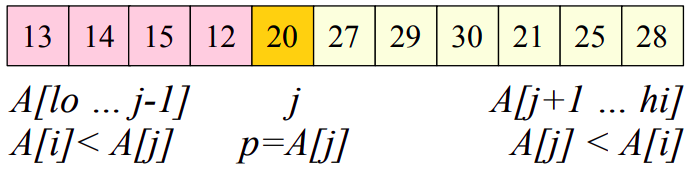
\includegraphics[width=0.7\textwidth]{quicksort1.png}
    \caption{Posizionamento dei valori dopo la scelta del \emph{pivot}}
\end{figure}\noindent
Nella fase di \emph{Impera} vengono ordinati i due sottoarray $A[lo\dots j-1]$
e $A[j+1\dots hi]$ e infine nella fare di \emph{Combina} non serve fare nulla in
quanto il vettore risulta già ordinato.

\begin{figure}[h!]
    \centering
    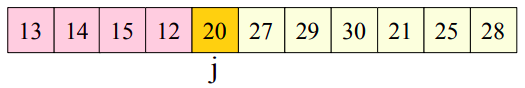
\includegraphics[width=0.7\textwidth]{quicksort2.png}
    \caption{Vettore ordinato al termine della fase di \emph{Impera}}
\end{figure}

\newpage
\subsection{Implementazione}
\begin{minicode}{Implementazione dell'algoritmo Quicksort}
    \ind quicksort(\bc{ITEM}[] A, \bc{int} lo, \bc{int} hi)\\
        \indf if (lo < hi) then\\
            \bc{int} j = pivot(A, lo, hi)\hfill\com{Calcola il \emph{pivot}}
            quicksort(A, lo, j - 1)\hfill\com{Ordina il sottoarray sinistro}
            quicksort(A, j + 1, hi)\hfill\com{Ordina il sottoarray destro}

    \com{Funzione per la ricerca del \emph{pivot}}
    \rmbreak\ind\bc{int} pivot(\bc{ITEM}[] A, \bc{int} lo, \bc{int} hi)\\
        \bc{ITEM} pivot = A[lo]\hfill\com{Scelta del valore del \emph{pivot}}
        \bc{int} j = lo\hfill\com{Indice del \emph{pivot}}
        \indf for (i = lo + 1 to hi) do\\
            \indff if (A[i] < pivot) then\\
                j = j + 1\hfill\com{Aggiorna l'indice del \emph{pivot}}
                swap(A, i, j)\hfill\com{Scambia di posizione gli elementi agli indici $i$ e $j$}
        \indf A[lo] = A[j]\\
        \indf A[j] = pivot\hfill\com{Mette in posizione $j$ il \emph{pivot}}
        \indf return j\\

    \com{Funzione ausiliaria per lo scambio di posizione di due elementi}
    \rmbreak\ind swap(\bc{ITEM}[] A, \bc{int} i, \bc{int} j)\\
        \bc{int} tmp = A[i]\\
        A[i] = A[j]\\
        A[j] = tmp
\end{minicode}

\subsection{Costo computazionale}
Per studiare il costo della funzione principale \texttt{quicksort} analizziamo
le funzioni ausiliarie. La \texttt{swap} è banale e ha un costo
$\Theta(1)$, mentre la \texttt{pivot} costa $\Theta(n)$ perché va a confrontare
il \emph{pivot} con ogni elemento dell'array. Per il costo della
\texttt{quicksort} consideriamo separatamente il caso pessimo il caso migliore.

\bigskip\noindent
Il caso pessimo è quello in cui la scelta del \emph{pivot} porta sempre ad avere
due sottoarray di dimensione $0$ e $n-1$ e conseguentemente induce una
\emph{funzione di ricorrenza} di questo tipo:
\[T(n)=T(n-1)+T(0)+\Theta(n)=T(n-1)+\Theta(n)=\Theta(n^2)\]
Nel caso migliore invece, il vettore viene sempre diviso in due sottoarray di
dimensione $n/2$ e quindi il costo è descritto dalla seguente funzione:
\[T(n)=2T(n/2)+\Theta(n)=\Theta(n\log n)\]

\bigskip\noindent
E il caso medio?
Fortunatamente, i partizionamenti nel caso medio sono molto più simili al caso
migliore che al peggiore. Ad esempio, con un partizionamento $9-a-1$ vale:
\[T(n)=T(n/10)+T(9n/10)+cn=\Theta(n\log n)\]
Lo stesso accade anche un partizionamento $99-a-1$:
\[T(n)=T(n/100)+T(99n/100)+cn=\Theta(n\log n)\]
\begin{note}
    In questi esempi non stiamo considerando i fattori moltiplicativi, ma in
    certi contesti potrebbero essere importanti.
\end{note}\noindent
Riassumendo, il costo dell'algoritmo \emph{Quicksort} è $\Theta(n\log n)$ nei
casi ottimo e medio, mentre è $\Theta(n^2)$ nel caso pessimo. Il \emph{Merge sort}
aveva un costo $\Theta(n\log n)$ in tutti i casi, quindi a prima vista
sembrerebbe essere più conveniente. In verità, poiché il \emph{Quicksort}
non usa memoria addizionale, gode di fattori moltiplicativi inferiori rispetto al
\emph{Merge sort}, è parallelizzabile ed esistono tecniche Euristiche che consentono
di evitare il caso pessimo, è spesso preferito al \emph{Merge sort}.

\paragraph{Funzione euristica per la selezione del pivot}
Vediamo di seguito un esempio di una funzione per la selezione del \emph{pivot}
in maniera euristica.

\begin{minicode}{Implementazione euristica della funzione pivot}
\ind\bc{int} pivot(\bc{ITEM}[] A, \bc{int} lo, \bc{int} hi)\\
    \bc{int} m = $\lfloor$(lo + hi) / 2$\rfloor$\\
    \indf if (A[lo] > A[hi]) then\\
        swap(A, lo, hi)\hfill\com{Sposta il massimo in ultima posizione}
    \indf if (A[m] > A[hi]) then\\
        swap(A, m, hi)\hfill\com{Sposta il massimo in ultima posizione}
    \indf if (A[m] > A[lo]) then\\
        swap(A, m, lo)\hfill\com{Sposta il mediano in prima posizione}
    \indf \bc{ITEM} pivot = A[lo]\\
    \indf\bc{int} j = lo\hfill\com{Indice del \emph{pivot}}
    \indf for (i = lo + 1 to hi) do\\
        \indff if (A[i] < pivot) then\\
            j = j + 1\hfill\com{Aggiorna l'indice del \emph{pivot}}
            swap(A, i, j)\hfill\com{Scambia di posizione gli elementi agli indici $i$ e $j$}
    \indf A[lo] = A[j]\\
    \indf A[j] = pivot\hfill\com{Mette in posizione $j$ il \emph{pivot}}
    \indf return j\\
\end{minicode}

\section{Esercizio di applicazione del Divide-et-impera}
\begin{problem}[Ricerca di un gap in un vettore]
    Dato un vettore $V$ contenente $n\geq 2$ interi, un gap è un indice $i$ con
    $1<i\leq n$ tale che $V[i-1]<V[i]$.
    \begin{itemize}
        \item Dimostrare che se $n\geq2$ e $V[1]<V[n]$, allora $V$ contiene
        sicuramente almeno un gap;
        \item Progettare un algoritmo che, dato un vettore $V$ contenente $n\geq 2$
        valori e tale che $V[1]<V[n]$, restituisce la posizione di un gap nel vettore;        
    \end{itemize}

    \bigskip\noindent
    Iniziamo dimostrando il primo punto.
    \begin{proof}[Dimostrazione]
        Supponiamo per assurdo che non esista alcun gap all'interno di $V$. Di
        conseguenza, deve per forza valere la seguente catena di disuguaglianze:
        \[V[1]\geq V[2]\geq\dots\geq V[n]\]
        Questo però è impossibile in quanto per ipotesi $V[1]<V[n]$ e quindi deve
        per forza esistere almeno un gap all'interno di $V$.
    \end{proof}

    \noindent
    Per il secondo punto proviamo a fare un ragionamento per induzione.
    Siano $i$ e $j$ due indici tali che $1\leq i<j\leq n$ e supponiamo che $V[i]
    <V[j]$. In base a questa definizione di $i$ e $j$, nel sottoarray $V[i\dots j]$
    ci sono almeno due elementi e il primo, $V[i]$, è minore dell'ultimo, $V[j]$.

    Proviamo a dimostrare per induzione sulla dimensione del sottoarray
    $V[i\dots j]$ che esiste almeno un gap.
    \paragraph{Caso base} $n = 2$ e quindi $j-i+1=2$, ovvero $i=j-1$. Da questo
    segue che $V[i]<V[j]\Leftrightarrow V[j-1]<V[j]$ e quindi alla posizione j
    esiste un gap.

    \paragraph{Passo induttivo} Ipotizziamo che dato un qualunque sottoarray
    $V[h\dots k]$, di dimensione $n'<n$ e tale che $V[h]<V[k]$, contenga
    un gap. A questo punto, se consideriamo un qualunque indice $m\in\,]i,j[$,
    si verificherà sicuramente almeno uno dei seguenti casi:
    \begin{itemize}
        \item $V[m]<V[j]$: per ipotesi induttiva, esiste sicuramente un gap
        all'interno di $V[m\dots j]$;
        \item $V[i]<V[m]$: per ipotesi induttiva, esiste sicuramente un gap
        all'interno di $V[i\dots m]$;
    \end{itemize} 

    Fatte queste considerazioni, possiamo usare la tecnica del Divide-et-impera
    per definire un algoritmo per la ricerca di gap:
    \begin{minicode}{Implementazione algoritmo Divide-et-impera per la ricerca di gap}
        \ind\bc{int} gap(\bc{int}[] V, \bc{int} n)\\
            return gaprec(V, 1, n)\\

        \ind\bc{int} gaprec(\bc{int}[] V, \bc{int} i, \bc{int} j)\\
            \indf if (j == i + 1) then\hfill\com{Caso base}
                return j\\
            \indf\bc{int} m = $\lfloor$(i + j) / 2$\rfloor$\hfill\com{Scelta dell'indice $m\in\,]i,j[$}
            \indf if (V[m] < V[j]) then\\
                return gaprec(V, m, j)\\
            \indf else\\
                return gaprec(V, i, m)
    \end{minicode}
\end{problem}
\chapter{Strutture dati specializzate}
Finora abbiamo esaminato una serie di \emph{strutture dati} e per ciascuna
ne abbiamo anche analizzato il costo delle operazioni. È possibile però
definire \emph{strutture dati speciali}, o per meglio dire \q{\emph{specializzate}},
nelle quali vengono implementate soltanto alcune delle operazioni e per questo
motivo quelle implementazioni possono essere realizzare in modo più efficiente.

In questo capitolo vedremo due esempi di \emph{strutture specializzate}: le
\emph{code a priorità} e gli \emph{insiemi disgiunti}.

\section{Code a priorità}
\begin{definition}[Coda a priorità]
    Una coda a priorità è una struttura dati astratta, simile a una coda, in
    cui ogni elemento possiede un valore che ne indica la \q{priorità} e che
    viene usato per stabilire l'ordine di estrazione degli elementi dalla
    struttura.
\end{definition}

\noindent
Esistono due tipi di \emph{code a priorità} (\emph{priority queue}):
\begin{itemize}
    \item \emph{Min-priority queue}: l'estrazione avviene per valori crescenti
    di priorità;
    \item \emph{Max-priority queue}: l'estrazione avviene per valori decrescenti
    di priorità;
\end{itemize}

\paragraph{Specifica}
\begin{code}{MINPRIORITYQUEUE}
    \com{Crea una \emph{coda a priorità} con capacità $n$}
    \bc{PRIORITYQUEUE} PriorityQueue(\bc{int} n)
    \nl\com{Restituisce \bc{true} se la \emph{coda a priorità} è vuota}
    \bc{boolean} isEmpty()
    \nl\com{Restituisce l'elemento minimo di una \emph{coda a priorità} non vuota}
    \bc{ITEM} min()
    \nl\com{Rimuove e restituisce l’elemento minimo di una \emph{coda a priorità} non vuota}
    \bc{deleteMin()}
    \nl\com{Inserisce l'elemento $x$ con priorità $p$ nella \emph{coda a priorità} e restituisce}
    \com{un oggetto \bc{PRIORITYITEM} che identifica $x$ all'interno della \emph{coda}}
    \bc{PRIORITYITEM} insert(\bc{ITEM} x, \bc{int} p)
    \nl\com{Diminuisce la priorità dell’oggetto identificato da $y$ portandola a $p$}
    decrease(\bc{PRIORITYITEM} y, \bc{int} p)
\end{code}
\begin{note}
    La specifica di una \emph{max-priority queue} è uguale, ma invece delle
    operazioni \texttt{min}, \texttt{deleteMin} e \texttt{decrease} ha
    \texttt{max}, \texttt{deleteMax} e \texttt{increase}.
\end{note}\noindent
Utilizzando le \emph{strutture dati} viste finora possiamo calcolare i seguenti
costi:
\begin{table}[h!]
\resizebox{\linewidth}{!}{
\centering
\renewcommand{\arraystretch}{1.3}
\begin{tabular}{|c|c|c|c|c|}
    \hline
    \textbf{Operazione} & $\begin{array}[c]{c}
        \textbf{Lista}\\
        \textbf{Vettore non ordinato}
    \end{array}$ & \textbf{Lista ordinata} & \textbf{Vettore ordinato} &
    \textbf{Albero Red-Black}\\
    \hline
    \textbf{min} & $O(n)$ & $O(1)$ & $O(1)$ & $O(\log n)$\\
    \hline
    \textbf{deleteMin} & $O(n)$ & $O(1)$ & $O(n)$ & $O(\log n)$\\
    \hline
    \textbf{insert} & $O(n)$ & $O(n)$ & $O(n)$ & $O(\log n)$\\
    \hline
    \textbf{decrease} & $O(n)$ & $O(n)$ & $O(\log n)$ & $O(\log n)$\\
    \hline
\end{tabular}}
\end{table}

\noindent
È possibile fare meglio di così?

La risposta è sì, utilizzando uno \emph{heap}, una \emph{struttura dati speciale}
che associa i vantaggi di un \emph{albero}, cioè la \emph{complessità} $O(\log n)$,
e la memorizzazione efficiente ottenibile con i normali vettori.

\subsection{Heap}
La \emph{struttura dati} dello \emph{heap} fu inventata da J. Williams nel
1964 con l'obiettivo di realizzare l'algoritmo di ordinamento \emph{HeapSort}.
Vediamo come si è arrivati all'ideazione dello \emph{heap}.

\bigskip\noindent
Consideriamo un \emph{albero binario perfetto} come il seguente:
\begin{figure}[h!]
    \centering
    \begin{graph}
        \node[main] (0) {$a$};
        \node[main] (1) [below left of=0, xshift=-10, yshift=-20] {$b$};
        \node[main] (2) [below right of=0, xshift=10, yshift=-20] {$c$};
        \node[main] (3) [below left of=1, xshift=10, yshift=-20] {$d$};
        \node[main] (4) [below right of=1, xshift=-10, yshift=-20] {$e$};
        \node[main] (5) [below left of=2, xshift=10, yshift=-20] {$f$};
        \node[main] (6) [below right of=2, xshift=-10, yshift=-20] {$g$};
      
        \path[-]  (0) edge (1)
                  (0) edge (2)
                  (1) edge (3)
                  (1) edge (4)
                  (2) edge (5)
                  (2) edge (6);
    \end{graph}
    \caption{\emph{Albero binario perfetto}}
\end{figure}

\noindent
Tutte le \emph{foglie} sono alla stessa \emph{profondità} $h$ e tutti i \emph{nodi}
interni hanno \emph{grado uscente} pari a 2. Se $n$ è il numero di \emph{nodi},
l'\emph{altezza} vale $h=\lfloor\log n\rfloor$ e, data l'\emph{altezza} $h$, il
numero di \emph{nodi} è $n=2^{h+1}-1$.

\bigskip\noindent
Cosa accade se si aggiunge un \emph{nodo}?

Ovviamente l'\emph{albero} non può più essere definito \emph{perfetto}. Supponiamo
però di \q{accatastare} tutti i nuovi \emph{nodi} a partire da sinistra. In questo
modo otteniamo un \emph{albero binario completo} nel quale tutte le \emph{foglie}
hanno \emph{profondità} $h$ o $h-1$, i \emph{nodi} al \emph{livello} $h$ sono
\q{accatastati} a sinistra e tutti \emph{nodi} interni hanno \emph{grado uscente}
pari a 2 eccetto al più uno. Come prima poi, per l'\emph{altezza} $h$ vale $h=\lfloor
\log n\rfloor$.

\begin{figure}[ht]
    \centering
    \begin{graph}
        \node[main] (0) {$a$};
        \node[main] (1) [below left of=0, xshift=-10, yshift=-20] {$b$};
        \node[main] (2) [below right of=0, xshift=10, yshift=-20] {$c$};
        \node[main] (3) [below left of=1, xshift=10, yshift=-20] {$d$};
        \node[main] (4) [below right of=1, xshift=-10, yshift=-20] {$e$};
        \node[main] (5) [below left of=2, xshift=10, yshift=-20] {$f$};
      
        \path[-]  (0) edge (1)
                  (0) edge (2)
                  (1) edge (3)
                  (1) edge (4)
                  (2) edge (5);
    \end{graph}
    \caption{\emph{Albero completo}}
\end{figure}
\begin{definition}[Albero min-heap]
    Un albero min-heap è un albero binario completo tale per cui il valore
    memorizzato in ogni nodo è minore dei valori memorizzati nei suoi figli.
\end{definition}
\begin{definition}[Albero max-heap]
    Un albero max-heap è un albero binario completo tale per  cui il valore
    memorizzato in ogni nodo è maggiore dei valori memorizzati nei suoi figli.
\end{definition}

\begin{figure}[th]
    \centering
    \begin{graph}
        \node[main] (0) {$16$};
        \node[main] (1) [below left of=0, xshift=-20, yshift=-20] {$14$};
        \node[main] (2) [below right of=0, xshift=20, yshift=-20] {$10$};
        \node[main] (3) [below left of=1, xshift=0, yshift=-20] {$8$};
        \node[main] (4) [below right of=1, xshift=0, yshift=-20] {$7$};
        \node[main] (5) [below left of=2, xshift=0, yshift=-20] {$9$};
        \node[main] (6) [below right of=2, xshift=0, yshift=-20] {$3$};
        \node[main] (7) [below left of=3, xshift=20, yshift=-20] {$2$};
        \node[main] (8) [below right of=3, xshift=-20, yshift=-20] {$4$};
        \node[main] (9) [below left of=4, xshift=20, yshift=-20] {$1$};
      
        \path[-]  (0) edge (1)
                  (0) edge (2)
                  (1) edge (3)
                  (1) edge (4)
                  (2) edge (5)
                  (2) edge (6)
                  (3) edge (7)
                  (3) edge (8)
                  (4) edge (9);
    \end{graph}
    \caption{\emph{Albero max-heap}}
\end{figure}\noindent
Un \emph{albero heap} non impone un ordinamento totale tra i \emph{figli} di un
\emph{nodo}, bensì definisce un \emph{ordinamento parziale} e quindi soddisfa
le seguenti tre proprietà:
\begin{itemize}
    \item \emph{Riflessività}: ogni \emph{nodo} è maggiore o uguale a se stesso;
    \item \emph{Antisimmetria}: se $n\geq m$ e $m\geq n$, allora $m=n$;
    \item \emph{Transitività}: se $n\geq m$ e $m\geq r$, allora $n\geq r$;
\end{itemize}
\begin{note}
    Un ordinamento parziale è una nozione più debole, ma più facile da
    realizzare.
\end{note}

\paragraph{Memorizzazione}
Un \emph{albero heap} può essere rappresentato mediante un \emph{vettore heap},
cioè un vettore nel quale, se la \emph{radice} è in posizione 1, il \emph{padre}
e i \emph{figli sinistro} e \emph{destro} di un \emph{nodo} in posizione $i$ si
trovano rispettivamente alle posizioni $p(i)=\lfloor i/2\rfloor$, $l(i)=2i$ e $r(i)=2i+i$.

Se invece la \emph{radice} è in posizione 0, gli indici del \emph{padre} e dei
\emph{figli} diventano rispettivamente $p(i)=\lfloor(i-1)/2\rfloor$, $l(i)=2i+1$
e $r(i)=2i+2$.

\begin{figure}[h!]
    \centering
    \subfloat[\emph{Albero heap} con \emph{radice} in 1]
    {
        \resizebox*{0.48\textwidth}{!}{
            \begin{graph}
                \node[main, label={$A[1]$}] (0) {$16$};
                \node[main, label={$A[2]$}] (1) [below left of=0, xshift=-20, yshift=-20] {$14$};
                \node[main, label={$A[3]$}] (2) [below right of=0, xshift=20, yshift=-20] {$10$};
                \node[main, label={$A[4]$}] (3) [below left of=1, xshift=0, yshift=-20] {$8$};
                \node[main, label={$A[5]$}] (4) [below right of=1, xshift=0, yshift=-20] {$7$};
                \node[main, label={$A[6]$}] (5) [below left of=2, xshift=0, yshift=-20] {$9$};
                \node[main, label={$A[7]$}] (6) [below right of=2, xshift=0, yshift=-20] {$3$};
                \node[main, label=below:{$A[8]$}] (7) [below left of=3, xshift=20, yshift=-20] {$2$};
                \node[main, label=below:{$A[9]$}] (8) [below right of=3, xshift=-20, yshift=-20] {$4$};
                \node[main, label=below:{$A[10]$}] (9) [below left of=4, xshift=20, yshift=-20] {$1$};
              
                \path[-]  (0) edge (1)
                          (0) edge (2)
                          (1) edge (3)
                          (1) edge (4)
                          (2) edge (5)
                          (2) edge (6)
                          (3) edge (7)
                          (3) edge (8)
                          (4) edge (9);
            \end{graph}
        }
    }
    \hfill
    \subfloat[\emph{Albero heap} con \emph{radice} in 0]
    {
        \resizebox*{0.48\textwidth}{!}{
            \begin{graph}
                \node[main, label={$A[0]$}] (0) {$16$};
                \node[main, label={$A[1]$}] (1) [below left of=0, xshift=-20, yshift=-20] {$14$};
                \node[main, label={$A[2]$}] (2) [below right of=0, xshift=20, yshift=-20] {$10$};
                \node[main, label={$A[3]$}] (3) [below left of=1, xshift=0, yshift=-20] {$8$};
                \node[main, label={$A[4]$}] (4) [below right of=1, xshift=0, yshift=-20] {$7$};
                \node[main, label={$A[5]$}] (5) [below left of=2, xshift=0, yshift=-20] {$9$};
                \node[main, label={$A[6]$}] (6) [below right of=2, xshift=0, yshift=-20] {$3$};
                \node[main, label=below:{$A[7]$}] (7) [below left of=3, xshift=20, yshift=-20] {$2$};
                \node[main, label=below:{$A[8]$}] (8) [below right of=3, xshift=-20, yshift=-20] {$4$};
                \node[main, label=below:{$A[9]$}] (9) [below left of=4, xshift=20, yshift=-20] {$1$};
              
                \path[-]  (0) edge (1)
                          (0) edge (2)
                          (1) edge (3)
                          (1) edge (4)
                          (2) edge (5)
                          (2) edge (6)
                          (3) edge (7)
                          (3) edge (8)
                          (4) edge (9);
            \end{graph}
        }
    }\\
    \subfloat[\emph{Vettore heap} con \emph{radice} in 1]
    {
        \resizebox*{0.48\textwidth}{!}{
            \begin{graph}
                \node[rectangle, draw, label={$A[1]$}, minimum width=10mm, minimum height=10mm]
                    (0) {\texttt{16}};
                \node[rectangle, draw, label={$A[2]$}, minimum width=10mm, minimum height=10mm]
                    (1) [right of=0, xshift=-28.5] {\texttt{14}};
                \node[rectangle, draw, label={$A[3]$}, minimum width=10mm, minimum height=10mm]
                    (2) [right of=1, xshift=-28.5] {\texttt{10}};
                \node[rectangle, draw, label={$A[4]$}, minimum width=10mm, minimum height=10mm]
                    (3) [right of=2, xshift=-28.5] {\texttt{8}};
                \node[rectangle, draw, label={$A[5]$}, minimum width=10mm, minimum height=10mm]
                    (4) [right of=3, xshift=-28.5] {\texttt{7}};
                \node[rectangle, draw, label={$A[6]$}, minimum width=10mm, minimum height=10mm]
                    (5) [right of=4, xshift=-28.5] {\texttt{9}};
                \node[rectangle, draw, label={$A[7]$}, minimum width=10mm, minimum height=10mm]
                    (6) [right of=5, xshift=-28.5] {\texttt{3}};
                \node[rectangle, draw, label={$A[8]$}, minimum width=10mm, minimum height=10mm]
                    (7) [right of=6, xshift=-28.5] {\texttt{2}};
                \node[rectangle, draw, label={$A[9]$}, minimum width=10mm, minimum height=10mm]
                    (8) [right of=7, xshift=-28.5] {\texttt{4}};
                \node[rectangle, draw, label={$A[10]$}, minimum width=10mm, minimum height=10mm]
                    (9) [right of=8,xshift=-28.5] {\texttt{1}};
            \end{graph}
        }
    }
    \hfill
    \subfloat[\emph{Vettore heap} con \emph{radice} in 0]
    {
        \resizebox*{0.48\textwidth}{!}{
            \begin{graph}
                \node[rectangle, draw, label={$A[0]$}, minimum width=10mm, minimum height=10mm]
                    (0) {\texttt{16}};
                \node[rectangle, draw, label={$A[1]$}, minimum width=10mm, minimum height=10mm]
                    (1) [right of=0, xshift=-28.5] {\texttt{14}};
                \node[rectangle, draw, label={$A[2]$}, minimum width=10mm, minimum height=10mm]
                    (2) [right of=1, xshift=-28.5] {\texttt{10}};
                \node[rectangle, draw, label={$A[3]$}, minimum width=10mm, minimum height=10mm]
                    (3) [right of=2, xshift=-28.5] {\texttt{8}};
                \node[rectangle, draw, label={$A[4]$}, minimum width=10mm, minimum height=10mm]
                    (4) [right of=3, xshift=-28.5] {\texttt{7}};
                \node[rectangle, draw, label={$A[5]$}, minimum width=10mm, minimum height=10mm]
                    (5) [right of=4, xshift=-28.5] {\texttt{9}};
                \node[rectangle, draw, label={$A[6]$}, minimum width=10mm, minimum height=10mm]
                    (6) [right of=5, xshift=-28.5] {\texttt{3}};
                \node[rectangle, draw, label={$A[7]$}, minimum width=10mm, minimum height=10mm]
                    (7) [right of=6, xshift=-28.5] {\texttt{2}};
                \node[rectangle, draw, label={$A[8]$}, minimum width=10mm, minimum height=10mm]
                    (8) [right of=7, xshift=-28.5] {\texttt{4}};
                \node[rectangle, draw, label={$A[9]$}, minimum width=10mm, minimum height=10mm]
                    (9) [right of=8,xshift=-28.5] {\texttt{1}};
            \end{graph}
        }
    }
    \caption{Memorizzazione \emph{alberi heap}}
\end{figure}

\noindent
Dalle definizioni di \emph{alberi min-heap} e \emph{max-heap} possiamo dedurre
delle proprietà sui relativi \emph{vettori}:
\begin{itemize}
    \item \emph{Vettori min-heap}: $A[i]\leq A[l(i)]$ e $A[i]\leq A[r(i)]$;
    \item \emph{Vettori max-heap}: $A[i]\geq A[l(i)]$ e $A[i]\geq A[r(i)]$;
\end{itemize}

\subsection{Algoritmo HeapSort}
Vediamo quindi l'algoritmo \emph{HeapSort} per l'ordinamento in senso crescente
di un vettore.

L'algoritmo ordina un vettore \q{in-place}, costruendo prima su di esso un
\emph{albero max-heap} e poi spostando progressivamente in fondo gli elemento massimi.
Ad ogni spostamento vengono ripristinate le proprietà degli \emph{alberi max-heap}.

Le funzioni utilizzate sono due:
\begin{itemize}
    \item \texttt{heapBuild}: costruisce un \emph{albero max-heap} a partire da
    un vettore non ordinato;
    \item \texttt{maxHeapRestore}: ripristina le proprietà degli \emph{alberi
    max-heap};
\end{itemize}
\begin{note}
    Tutte le operazioni vengono effettuate \q{in-place}, cioè agiscono sul vettore
    stesso senza usare \emph{strutture ausiliarie}. Quindi, l'\emph{albero max-heap}
    non viene realmente creato, ma grazie alle sue proprietà di memorizzazione,
    il vettore di input viene semplicemente interpretato come fosse un \emph{albero
    max-heap}.
\end{note}
Per questo motivo, la funzione \emph{maxHeapRestore} riceve in input un vettore $A$
e un indice $i$ e si occupa di garantire che al termine dell'esecuzione,
l'\emph{albero binario} con radice $i$ sia un \emph{albero max-heap}.

\begin{eg}[Esempio di esecuzione della maxHeapRestore]
    Consideriamo il seguente vettore:
    \[(3,\,14,\,10,\,8,\,7,\,9,\,5,\,2,\,4,\,1)\]
    e ipotizziamo di invocare \texttt{maxHeapRestore} su di esso usando come
    radice la posizione $1$.

    \begin{figure}[h!]
        \centering
        \subfloat[Situazione iniziale]
        {
            \resizebox*{0.48\textwidth}{!}{
                \begin{graph}
                    \node[main, fill=leaf, line width=1.2pt] (0) {$3$};
                    \node[main] (1) [below left of=0, xshift=-20, yshift=-20] {$14$};
                    \node[main] (2) [below right of=0, xshift=20, yshift=-20] {$10$};
                    \node[main] (3) [below left of=1, xshift=0, yshift=-20] {$8$};
                    \node[main] (4) [below right of=1, xshift=0, yshift=-20] {$7$};
                    \node[main] (5) [below left of=2, xshift=0, yshift=-20] {$9$};
                    \node[main] (6) [below right of=2, xshift=0, yshift=-20] {$5$};
                    \node[main] (7) [below left of=3, xshift=20, yshift=-20] {$2$};
                    \node[main] (8) [below right of=3, xshift=-20, yshift=-20] {$4$};
                    \node[main] (9) [below left of=4, xshift=20, yshift=-20] {$1$};
                  
                    \path[-]  (0) edge (1)
                              (0) edge (2)
                              (1) edge (3)
                              (1) edge (4)
                              (2) edge (5)
                              (2) edge (6)
                              (3) edge (7)
                              (3) edge (8)
                              (4) edge (9);
                \end{graph}
            }
        }
        \hfill
        \subfloat[Il 3 viene scambiato con il 14]
        {
            \resizebox*{0.48\textwidth}{!}{
                \begin{graph}
                    \node[main] (0) {$14$};
                    \node[main, fill=leaf, line width=1.2pt] (1) [below left of=0, xshift=-20, yshift=-20] {$3$};
                    \node[main] (2) [below right of=0, xshift=20, yshift=-20] {$10$};
                    \node[main] (3) [below left of=1, xshift=0, yshift=-20] {$8$};
                    \node[main] (4) [below right of=1, xshift=0, yshift=-20] {$7$};
                    \node[main] (5) [below left of=2, xshift=0, yshift=-20] {$9$};
                    \node[main] (6) [below right of=2, xshift=0, yshift=-20] {$5$};
                    \node[main] (7) [below left of=3, xshift=20, yshift=-20] {$2$};
                    \node[main] (8) [below right of=3, xshift=-20, yshift=-20] {$4$};
                    \node[main] (9) [below left of=4, xshift=20, yshift=-20] {$1$};
                  
                    \path[-]  (0) edge (1)
                              (0) edge (2)
                              (1) edge (3)
                              (1) edge (4)
                              (2) edge (5)
                              (2) edge (6)
                              (3) edge (7)
                              (3) edge (8)
                              (4) edge (9);

                    \path[->, dashed]   (0) edge[bend left=30] (1)
                                        (1) edge[bend left=30] (0);
                \end{graph}
            }
        }\\
        \subfloat[Il 3 viene scambiato con l'8]
        {
            \resizebox*{0.48\textwidth}{!}{
                \begin{graph}
                    \node[main] (0) {$14$};
                    \node[main] (1) [below left of=0, xshift=-20, yshift=-20] {$8$};
                    \node[main] (2) [below right of=0, xshift=20, yshift=-20] {$10$};
                    \node[main, fill=leaf, line width=1.2pt] (3) [below left of=1, xshift=0, yshift=-20] {$3$};
                    \node[main] (4) [below right of=1, xshift=0, yshift=-20] {$7$};
                    \node[main] (5) [below left of=2, xshift=0, yshift=-20] {$9$};
                    \node[main] (6) [below right of=2, xshift=0, yshift=-20] {$5$};
                    \node[main] (7) [below left of=3, xshift=20, yshift=-20] {$2$};
                    \node[main] (8) [below right of=3, xshift=-20, yshift=-20] {$4$};
                    \node[main] (9) [below left of=4, xshift=20, yshift=-20] {$1$};
                  
                    \path[-]  (0) edge (1)
                              (0) edge (2)
                              (1) edge (3)
                              (1) edge (4)
                              (2) edge (5)
                              (2) edge (6)
                              (3) edge (7)
                              (3) edge (8)
                              (4) edge (9);

                    \path[->, dashed]   (1) edge[bend left=30] (3)
                                        (3) edge[bend left=30] (1);
                \end{graph}
            }
        }
        \hfill
        \subfloat[Il 3 viene scambiato con il 4]
        {
            \resizebox*{0.48\textwidth}{!}{
                \begin{graph}
                    \node[main] (0) {$14$};
                    \node[main] (1) [below left of=0, xshift=-20, yshift=-20] {$8$};
                    \node[main] (2) [below right of=0, xshift=20, yshift=-20] {$10$};
                    \node[main] (3) [below left of=1, xshift=0, yshift=-20] {$4$};
                    \node[main] (4) [below right of=1, xshift=0, yshift=-20] {$7$};
                    \node[main] (5) [below left of=2, xshift=0, yshift=-20] {$9$};
                    \node[main] (6) [below right of=2, xshift=0, yshift=-20] {$5$};
                    \node[main] (7) [below left of=3, xshift=20, yshift=-20] {$2$};
                    \node[main, fill=leaf, line width=1.2pt] (8) [below right of=3, xshift=-20, yshift=-20] {$3$};
                    \node[main] (9) [below left of=4, xshift=20, yshift=-20] {$1$};
                  
                    \path[-]  (0) edge (1)
                              (0) edge (2)
                              (1) edge (3)
                              (1) edge (4)
                              (2) edge (5)
                              (2) edge (6)
                              (3) edge (7)
                              (3) edge (8)
                              (4) edge (9);
                  
                    \path[->, dashed]   (3) edge[bend left=30] (8)
                                        (8) edge[bend left=30] (3);
                \end{graph}
            }
        }
    \end{figure}\noindent
    Al termine dell'esecuzione abbiamo ottenuto un albero max-heap corretto.
\end{eg}

\newpage
\paragraph{Implementazione}
\begin{minicode}{Implementazione maxHeapRestore}
    \ind maxHeapRestore(\bc{ITEM}[] A, \bc{int} i, \bc{int} dim)\\
        \bc{int} max = i\hfill\com{Sceglie la \emph{radice}}
        \indf if (l(i) $\leq$ dim A[l(i)] > A[max]) then\\
            max = l(i)\\
        \indf if (r(i) $\leq$ dim A[r(i)] > A[max]) then\\
            max = r(i)\\
        \indf if (i $\neq$ max) then\hfill\com{Se $i == max$ l'\emph{albero} è apposto}
            swap(A, i, max)\hfill\com{Scambia la \emph{radice} e il maggiore tra i suoi \emph{figli}}
            maxHeapRestore(A, max, dim)\hfill\com{Controlla il \emph{sottoalbero} con \emph{radice} $max$}
\end{minicode}
\paragraph{Complessità}
Ad ogni chiamata vengono eseguiti $O(1)$ confronti e se il \emph{nodo} $i$ non è
massimo, si invoca ricorsivamente \texttt{maxHeapRestore} su uno dei \emph{figli}.
L'esecuzione nel caso peggiore termina al raggiungimento di una \emph{foglia},
quindi il costo è limitato dall'\emph{altezza} dell'\emph{albero}, ovvero
$T(n)=O(\log n)$.

\paragraph{Dimostrazione di correttezza}
\begin{proof}[Dimostrazione]
    Dobbiamo dimostrare che al termine dell'esecuzione l'\emph{albero} con
    \emph{radice} in $A[i]$ rispetta le proprietà degli \emph{alberi max-heap}.
    Procediamo per induzione sull'\emph{altezza} $h$ dell'\emph{albero}.

    \paragraph{Caso base} $h=0$. L'\emph{albero} è composto da un solo
    \emph{nodo} e quindi rispetta per forza le proprietà.
    \paragraph{Passo induttivo} Ipotizziamo che l'algoritmo funzioni correttamente
    su tutti gli \emph{alberi} di \emph{altezza} minore di $h$. A questo punto si
    configurano tre casi:
    \begin{itemize}
        \item \emph{Caso 1}: $A[i]\geq A[l(i)]$ e $A[i]\geq A[r(i)]$, ovvero
        il \emph{nodo} $A[i]$ è più grande dei propri \emph{figli} e quindi
        l'\emph{albero radicato} in $A[i]$ è un \emph{albero max-heap} e l'algoritmo
        termina;
        \item \emph{Caso 2}: $A[i]<A[l(i)]$ e $A[r(i)]<A[l(i)]$, ovvero il \emph{figlio
        sinistro} è più grande sia del \emph{padre} che del \emph{fratello}. Quindi,
        vengono scambiati di posizione il \emph{figlio sinistro} e il \emph{padre}.
        A questo punto valgono $A[i]\geq A[l(i)]$ e $A[i]\geq A[r(i)]$, ma il
        \emph{sottoalbero} con \emph{radice} in $A[l(i)]$ potrebbe non rispettare
        più le proprietà per gli \emph{alberi max-heap}. Di conseguenza, l'algoritmo
        continua applicando ricorsivamente \texttt{maxHeapRestore} sull'\emph{albero}
        con \emph{radice} in $A[l(i)]$, ma siccome quell'\emph{albero} ha \emph{altezza}
        minore di $h$, per ipotesi induttiva, l'algoritmo riesce correttamente a
        garantire il rispetto di tutte le proprietà;
        \item \emph{Caso 3}: $A[i]<A[r(i)]$ e $A[l(i)]<A[r(i)]$, ovvero il \emph{figlio
        destro} è più grande sia del \emph{padre} che del \emph{fratello}. Quindi,
        vengono scambiati di posizione il \emph{figlio destro} e il \emph{padre}.
        A questo punto valgono $A[i]\geq A[l(i)]$ e $A[i]\geq A[r(i)]$, ma il
        \emph{sottoalbero} con \emph{radice} in $A[r(i)]$ potrebbe non rispettare
        più le proprietà per gli \emph{alberi max-heap}. Di conseguenza, l'algoritmo
        continua applicando ricorsivamente \texttt{maxHeapRestore} sull'\emph{albero}
        con \emph{radice} in $A[r(i)]$, ma siccome quell'\emph{albero} ha \emph{altezza}
        minore di $h$, per ipotesi induttiva, l'algoritmo riesce correttamente a
        garantire il rispetto di tutte le proprietà;
    \end{itemize}
\end{proof}\noindent
Consideriamo ora la funzione \texttt{heapBuild}. La funzione riceve in input un
vettore da ordinare e, per le proprietà di memorizzazione degli \emph{alberi heap},
sappiamo che tutti i \emph{nodi} con indici compresi tra $\lfloor n/2\rfloor+1$
e $n$ sono \emph{foglie}, ovvero \emph{alberi heap} contenenti un solo elemento.

La funzione \texttt{heapBuild} quindi, non fa altro che applicare \texttt{maxHeapRestore}
a tutti i \emph{nodi}, partendo dal primo che non è una \emph{foglia}, cioè da
$A[\lfloor n/2\rfloor]$, e risalendo fino alla \emph{radice}.

\paragraph{Implementazione}
\begin{minicode}{Implementazione heapBuild}
    \ind heapBuild(\bc{ITEM}[] A, \bc{int} n)\\
        \indf for (i = $\lfloor$n/2$\rfloor$ downto 1) do\\
            maxHeapRestore(A, i, n)
\end{minicode}
\begin{figure}[h!]
    \centering
    \begin{graph}
        \node[main, label={$A[1]$}] (0) {$14$};
        \node[main, label={$A[2]$}] (1) [below left of=0, xshift=-20, yshift=-20] {$45$};
        \node[main, label={$A[3]$}] (2) [below right of=0, xshift=20, yshift=-20] {$28$};
        \node[main, label={$A[4]$}] (3) [below left of=1, xshift=0, yshift=-20] {$34$};
        \node[main, label={$A[5]$}] (4) [below right of=1, xshift=0, yshift=-20] {$15$};
        \node[main, fill=leaf, label={$A[6]$}] (5) [below left of=2, xshift=0, yshift=-20] {$20$};
        \node[main, fill=leaf, label={$A[7]$}] (6) [below right of=2, xshift=0, yshift=-20] {$22$};
        \node[main, fill=leaf, label=below:{$A[8]$}] (7) [below left of=3, xshift=20, yshift=-20] {$30$};
        \node[main, fill=leaf, label=below:{$A[9]$}] (8) [below right of=3, xshift=-20, yshift=-20] {$21$};
        \node[main, fill=leaf, label=below:{$A[10]$}] (9) [below left of=4, xshift=20, yshift=-20] {$25$};
        \node[main, fill=leaf, label=below:{$A[11]$}] (10) [below right of=4, xshift=-20, yshift=-20] {$16$};
      
        \path[-]  (0) edge (1)
                  (0) edge (2)
                  (1) edge (3)
                  (1) edge (4)
                  (2) edge (5)
                  (2) edge (6)
                  (3) edge (7)
                  (3) edge (8)
                  (4) edge (9)
                  (4) edge (10);
    \end{graph}
    \caption{\texttt{maxHeapRestore} viene applicata solo ai \emph{nodi} interni}
\end{figure}
\paragraph{Dimostrazione di correttezza}
\begin{proof}[Dimostrazione]
    Dimostriamo la seguente \emph{invariante di ciclo}:
    
    \smallskip\noindent {\em All'inizio di ogni iterazione del ciclo \texttt{for},
    i nodi $[i+1\dots n]$ sono radici di alberi heap.}
    \paragraph{Inizializzazione}
    All'inizio $i=\lfloor n/2\rfloor$. Supponiamo che $\lfloor n/2\rfloor+1$ non
    sia una \emph{foglia} e che quindi abbia almeno il \emph{figlio sinistro}.
    Se così fosse, il \emph{figlio} dovrebbe trovarsi alla posizione $2(\lfloor
    n/2\rfloor+1)=2\lfloor n/2\rfloor+2$, ma ciò sarebbe assurdo perché le posizioni
    $n+1$ e $n+2$ eccedono la dimensione massima che $n$. La stessa dimostrazione
    vale anche per tutti gli indici successivi.
    \paragraph{Conservazione}
    È possibile applicare \texttt{maxHeapRestore} a ogni \emph{nodo} $i\in[\lfloor
    n/2\rfloor+1\dots n]$ perché entrambi i \emph{nodi} alle posizioni $2i<2i+1\leq
    n$ sono \emph{radici} di \emph{alberi heap}. Al termine di ogni iterazioni,
    i \emph{nodi} $[i\dots n]$ sono \emph{radici} di \emph{alberi heap}.
    \paragraph{Conclusione} Al termine, $i=0$ e quindi il \emph{nodo} $1$ è
    \emph{radice} di un \emph{albero heap}.
\end{proof}
\paragraph{Complessità}
Sicuramente possiamo dire che \texttt{heapBuild} è un $O(n\log n)$ in quanto il costo
di \texttt{maxHeapRestore} è $O(\log n)$ e viene invocata $\lfloor n/2\rfloor=O(n)$
volte. Ma è veramente questo il costo?

\bigskip\noindent
In realtà, le operazioni \texttt{maxHeapRestore} vengono eseguite un
numero decrescente di volte in un \emph{albero} di \emph{altezza} crescente. E in
particolare, vale la seguente tabella:

\begin{table}[h!]
    \centering
    \renewcommand{\arraystretch}{1.2}
    \begin{tabular}{|c|c|}
        \hline
        \textbf{Altezza} & \textbf{\# esecuzioni}\\
        \hline
        0 & $\lfloor n/2^1\rfloor$\\
        \hline
        1 & $\lfloor n/2^2\rfloor$\\
        \hline
        2 & $\lfloor n/2^3\rfloor$\\
        \hline
        \dots & \dots\\
        \hline
        $h$ & $\lfloor n/2^{h+1}\rfloor$\\
        \hline
    \end{tabular}
\end{table}\noindent
Se questo è vero, possiamo scrivere la \emph{funzione di ricorrenza} come:
\[T(n)\begin{array}[t]{cll}
    \leq & \sum_{h=1}^{\lfloor n/2\rfloor}\frac{n}{2^{h+1}}h\\
    = & n\sum_{h=1}^{\lfloor n/2\rfloor}\left(\frac{1}{2}\right)^{h+1}h\\
    = & \frac{n}{2}\sum_{h=1}^{\lfloor n/2\rfloor}\left(\frac{1}{2}\right)^{h}h\\
    \leq & \frac{n}{2}\sum_{h=1}^{+\infty}\left(\frac{1}{2}\right)^{h}h & \quad\emph{Estensione ad infinito della somamtoria}\\
    = & \frac{n}{2}\frac{\frac{1}{2}}{\left(1-\frac{1}{2}\right)^2} & \quad\hyperlink{ser:5}{\emph{Serie geometrica infinita decrescente}}\\
    = & \frac{n}{2}\frac{\frac{1}{2}}{\left(\frac{1}{2}\right)^2}\\
    = & \frac{n}{2}2\\
    = & n = O(n)
\end{array}\]

\paragraph{Implementazione}
\begin{minicode}{Implementazione dell'algoritmo HeapSort}
    \ind heapsort(\bc{ITEM}[] A, \bc{int} n)\\
        heapBuild(A, n)\\
        \indf for (i = n downto 2) do\\
            swap(A, 1, i)\hfill\com{L'elemento massimo viene spostato in fondo}
            maxHeapRestore(A, 1, n - 1)\hfill\com{Ripristina le proprietà}
\end{minicode}\noindent
In pratica, l'\emph{HeapSort} inizia costruendo un \emph{albero max-heap} sul
vettore da ordinare. Ad ogni ciclo il primo elemento sarà sicuramente il
massimo e quindi viene scambiato di posto con l'elemento in posizione $i$.
Dopo ogni scambio viene invocata \texttt{maxHeapRestore} per ripristinare le
proprietà degli \emph{alberi max-heap}. Il tutto viene ripetuto fino a quando
$i$ non diventa 1.

\paragraph{Complessità}
La funzione \texttt{heapBuild} costa $\Theta(n)$, mentre le \texttt{maxHeapRestore}
ha un costo $\Theta(\log i)$ per $i$ che varia da $n$ a 2. La \emph{funzione di
ricorrenza} è la seguente:
\[T(n)=\sum_{i=n}^2\log i+\Theta(n)=\Theta(n\log n)\]

\paragraph{Dimostrazione di correttezza}
\begin{proof}[Dimostrazione]
    Dimostriamo la seguente \emph{invariante di ciclo}:
    
    \smallskip\noindent{\em All'inizio di ogni passo $i$ il sottovettore
    $A[i+1\dots n]$ è ordinato e ogni elemento in $A[1\dots i]$ è minore o
    al più uguale a ogni elemento in $A[i+1\dots n]$. Inoltre, l'elemento $A[1]$
    è la radice di un albero heap di dimensione $i$.}
    \paragraph{Inizializzazione}
    Dopo la \texttt{heapBuild} il primo elemento è la \emph{radice} di un
    \emph{albero max-heap} e quindi è maggiore dei propri \emph{figli} e, per la
    proprietà transitiva, anche dei \emph{figli} dei \emph{figli} fino alle
    \emph{foglie}. Alla prima iterazione quindi, $A[1]$ è il massimo e viene
    scambiato di posto con $A[i]=A[n]$. A quel punto, $A[n]$ è l'elemento
    massimo e il sottovettore $A[1\dots n-1]$ viene riorganizzato secondo le
    regole della \texttt{maxHeapRestore} portandone il massimo in $A[1]$.
    \paragraph{Conservazione}
    Per ogni $i\in[2\dots n]$, il sottovettore $A[i+1\dots n]$ è ordinato
    in senso crescente e in posizione $A[1]$ si trova l'elemento massimo del
    sottovettore $A[1\dots i]$. Al termine dell'iterazione, $A[i\dots n]$ è
    ordinato e $A[1]$ è il massimo in $A[1\dots i-1]$.
    \paragraph{Conclusione}
    Al termine, $i=1$ e quindi il sottovettore $A[2\dots n]$ è ordinato. Poiché
    vale sicuramente $A[1]\leq A[2]$, possiamo dire che tutto il vettore $A[1\dots
    n]$ è ordinato in senso crescente.
\end{proof}

\subsection{Implementazione di code a priorità}
Prima di vedere l'implementazione di una \emph{coda a priorità}, vediamo la
definizione di un \texttt{\bc{PRIORITYITEM}} e l'implementazione della funzione
\texttt{swap}.
\begin{minicode}{PRIORITYITEM}
    \bc{int} priority\hfill\com{Valore di priorità}
    \bc{ITEM} value\hfill\com{Valore}
    \bc{int} pos\hfill\com{Posizione nel vettore}
\end{minicode}
\begin{minicode}{Implementazione funzione swap}
    \ind swap(\bc{PRIORITYITEM} H, \bc{int} i, \bc{int} j)\\
        \bc{PRIORITYITEM} temp = H[i]\\
        H[i] = H[j]\\
        H[j] = temp\\
        H[i].pos = i\\
        H[j].pos = j
\end{minicode}\noindent
Di seguito quindi, vediamo l'implementazione di una \emph{min-priority queue}
come vettore di coppie $\langle valore,\,\emph{priorità}\rangle$. Ovviamente,
tutto ciò che vedremo vale simmetrico per le \emph{max-priority queue}.
\begin{minicode}{{Min-priority queue}}
    \bc{int} capacity\hfill\com{Dimensione massima della \emph{coda}}
    \bc{int} dim\hfill\com{Numero di elementi attualmente presenti nella \emph{coda}}
    \bc{PRIORITYQUEUE}[] H\hfill\com{\emph{Vettore heap}}
\end{minicode}
\newpage
\begin{codecont}
    \ind\bc{PRIORITYQUEUE} PriorityQueue(\bc{int} n)\\
        \bc{PRIORITYQUEUE} t = new \bc{PRIORITYQUEUE}\\
        t.capacity = n\\
        t.dim = 0\\
        t.H = new \bc{PRIORITYITEM}[1\dots n]\\
        return t\\

    \ind\bc{PRIORITYITEM} insert(\bc{ITEM} x, \bc{int} p)\\
        precondition: dim < capacity\\
        dim = dim + 1\\
        H[dim] = new \bc{PRIORITYITEM}\hfill\com{Aggiunge l'elemento in fondo}
        H[dim].value = x\\
        H[dim].priority = p\\
        H[dim].pos = dim\\
        \bc{int} i = dim\\
        \indf while (i > 1 and H[i].priority < H[p(i)].priority) do\\
            \indff swap(H, i, p(i))\hfill\com{Sposta il nuovo elemento nella posizione giusta}
            \indff i = p(i)\\
        \indf return H[i]\\

    \ind minHeapRestore(\bc{PRIORITYITEM}[] A, \bc{int} i, \bc{int} n)\\
        \bc{int} min = i\\
        if (l(i) $\leq$ dim and A[l(i)].priority < A[min].priority) then\\
            \indf min = l(i)\\
        \ind if (r(i) $\leq$ dim and A[r(i)].priority < A[min].priority) then\\
            \indf min = r(i)\\
        \ind if (i $\neq$ min) then\\
            \indf swap(A, i, min)\\
            \indf minHeapRestore(A, min, dim)\\

    \ind\bc{ITEM} deleteMin()\\
        precondition: dim > 0\\
        swap(H, 1, dim)\hfill\com{Scambia il primo e l'ultimo elemento}
        dim = dim - 1\\
        minHeapRestore(H, 1, dim)\hfill\com{Ripristina le proprietà}
        return H[dim + 1].value\hfill\com{Restituisce il valore dell'elemento rimosso}

    \ind\bc{ITEM} min()\\
        precondition: dim > 0\\
        return H[1].value\\
    
    \ind decrease(\bc{PRIORITYITEM} x, \bc{int} p)\\
        precondition: p < x.priority\\
        x.priority = p\\
        \bc{int} i = x.pos\\
        while (i > 1 and H[i].priority < H[p(i)].priority) do\\
            \indf swap(H, i, p(i))\hfill\com{Sposta l'elemento modificato nella posizione giusta}
            \indf i = p(i)
\end{codecont}
\paragraph{Complessità}
Tutte le operazioni che modificano gli \emph{heap} ne ripristinano anche le
proprietà. In particolare, questo viene fatto nel \emph{cammino radice-foglia}
dalla \texttt{deleteMin} e in quello \emph{nodo-radice} dalla \texttt{insert}
e dalla \texttt{decrease}. Poiché l'\emph{altezza} è $\lfloor\log n\rfloor$, il
costo di tali operazioni è $O(\log n)$.

\bigskip\noindent
La \emph{complessità} di tutte le operazioni è riassunta dalla seguente tabella:
\begin{table}[h!]
    \centering
    \renewcommand{\arraystretch}{1.2}
    \begin{tabular}{|c|c|}
        \hline
        \textbf{Operazione} & \textbf{Costo}\\
        \hline
        \texttt{insert} & $O(\log n)$\\
        \hline
        \texttt{deleteMin} & $O(\log n)$\\
        \hline
        \texttt{min} & $\Theta(1)$\\
        \hline
        \texttt{decrease} & $O(\log n)$\\
        \hline
    \end{tabular}
\end{table}

\section{Insiemi disgiunti}
In alcune applicazioni (e.g. ricerca delle \emph{componenti connesse} di un
\emph{grafo}) siamo interessati a gestire una collezione $S=\{S_1,\dots,
S_n\}$ di \emph{insiemi dinamici disgiunti}, ovvero tali per cui:
\[S_i\cap S_j=\emptyset\quad\forall i,j : i\neq j\]
\[\bigcup_{1=1}^n S_i=S\quad\text{con}\ n=\left|S\right|\]
Definiamo quindi la struttura dati \emph{merge-find set} con le seguenti primitive:
\begin{itemize}
    \item Creazione di $n$ \emph{insiemi disgiunti} composti da un elemento
    ciascuno;
    \item \texttt{find}: identificazione dell'\emph{insieme} a cui appartiene un
    elemento;
    \item \texttt{merge}: unione di due \emph{insiemi};
\end{itemize}\noindent
Ogni insieme è identificato da un proprio elemento che viene designato come
\emph{rappresentante}. Di conseguenza, la primitiva \texttt{find} deve restituire
il \emph{rappresentante} dell'\emph{insieme} in cui si trova elemento cercato.
Definito l'elemento \emph{rappresentante}, questo può essere cambiato solo in
caso di unione con un altro \emph{insieme}.

\begin{note}
    Per semplicità di esposizione, ipotizziamo che gli elementi siano identificati
    da un valore intero $1\dots n$ e che l'associazione con il valore vero e
    proprio sia memorizzata esternamente.
\end{note}

\paragraph{Specifica}
\begin{code}{Merge-find set}
    \com{Crea $n$ \emph{insiemi} $\{1\},\dots,\{n\}$}
    \bc{MFSET} Mfset(\bc{int} n)\\
    \com{Restituisce il \emph{rappresentante} dell'\emph{insieme} contenente $x$}
    \bc{int} find(\bc{int} x)\\
    \com{Unisce gli \emph{insiemi} che contengono $x$ e $y$}
    merge(\bc{int} x, \bc{int} y)
\end{code}

\newpage
\begin{eg}[Esempio di utilizzo di un merge-find set]
\mbox{}\begin{figure}[h!]
\centering
\begin{graph}
    \tikzset{rect/.style={draw, rectangle, minimum size=5mm,
            rounded corners=0.25cm, inner sep=4mm}}
    \node[rect] (1)                 {\bm{$1$}};
    \node[rect] (2) [right of=1]    {\bm{$2$}};
    \node[rect] (3) [right of=2]    {\bm{$3$}};
    \node[rect] (4) [right of=3]    {\bm{$4$}};
    \node[rect] (5) [right of=4]    {\bm{$5$}};
    \node[rect] (6) [right of=5]    {\bm{$6$}};

    \node[rect] (12) [below of=1, xshift=9.9mm, minimum width=30.3mm,
        inner sep=3.7mm] {\bm{$1$}$,2$};
    \node[rect] (3b) [below of=3]    {\bm{$3$}};
    \node[rect] (4b) [below of=4]    {\bm{$4$}};
    \node[rect] (5b) [below of=5]    {\bm{$5$}};
    \node[rect] (6b) [below of=6]    {\bm{$6$}};

    \node[rect] (12c) [below of=12, minimum width=30.3mm,
        inner sep=3.7mm] {\bm{$1$}$,2$};
    \node[rect] (34) [below of=3b, xshift=9.9mm, minimum width=30.3mm,
        inner sep=3.7mm] {\bm{$3$}$,4$};
    \node[rect] (5c) [below of=5b]    {\bm{$5$}};
    \node[rect] (6c) [below of=6b]    {\bm{$6$}};

    \node[rect] (12c) [below of=12c, minimum width=30.3mm,
        inner sep=3.7mm] {\bm{$1$}$,2$};
    \node[rect] (34d) [below of=34, minimum width=30.3mm,
        inner sep=3.7mm] {\bm{$3$}$,4$};
    \node[rect] (56) [below of=5c, xshift=9.9mm, minimum width=30.3mm,
        inner sep=3.7mm] {\bm{$5$}$,6$};

    \node[rect] (123)[below of=12c, xshift=20mm, minimum width=70.3mm,
        inner sep=3.7mm] {\bm{$1$}$,2,3,4$};
    \node[rect] (56e) [below of=56, minimum width=30.3mm,
        inner sep=3.7mm] {\bm{$5$}$,6$};

    \node[rect] (f) [below of=123, xshift=20mm, minimum width=110.3mm,
        inner sep=3.7mm] {\bm{$1$}$,2,3,4,5,6$};

    \node[] (l1) [right of=6] {\texttt{Mfset(6)}};
    \node[] (l2) [below of=l1, xshift=3mm] {\texttt{merge(1,2)}};
    \node[] (l3) [below of=l2] {\texttt{merge(3,4)}};
    \node[] (l4) [below of=l3] {\texttt{merge(5,6)}};
    \node[] (l5) [below of=l4] {\texttt{merge(1,3)}};
    \node[] (l6) [below of=l5] {\texttt{merge(1,5)}};
\end{graph}
\end{figure}
\end{eg}

\noindent
Utilizzando la struttura dati così definita, possiamo semplificare molto
l'algoritmo per la ricerca delle \emph{componenti connesse} di un \emph{grafo}
$G=(V,E)$. In particolare, è sufficiente inizializzare la struttura vedendo ogni
\emph{nodo} come un \emph{insieme}, quindi procedere ad unire \texttt{merge(u,v)}
per ogni \emph{arco} $(u,v)\in E$. Al termine, ogni \emph{insieme disgiunto}
rappresenterà una \emph{componente connesse}.

\begin{minicode}{Ricerca delle componenti connesse con merge-find set}
    \ind\bc{MFSET} cc(\bc{GRAPH} G)\\
        \bc{MFSET} M = Mfset(G.size())\\
        \indf foreach (u $\in$ G.V()) do\\
            \indff foreach (v $\in$ G.adj(u)) do\\
                M.merge(u,v)\\
        \indf return M
\end{minicode}\noindent
La \emph{complessità} di questa versione è $T(n)=O(n+m)$ dove $m$ è il numero di
invocazioni di \texttt{merge}.

\begin{note}
    Questa versione dell'algoritmo è particolarmente indicata nel caso di
    \emph{grafi dinamici} ovvero \emph{grafi} nei quali vengono spesso aggiunti
    nuovi \emph{archi}.
\end{note}

\bigskip\noindent
Ma quanto costa eseguire una \texttt{merge} e come è implementata?

Ci sono diverse implementazioni possibili tra le quali implementazioni basate su
\emph{insiemi di liste} e su \emph{insiemi di alberi} (i.e. \emph{foreste}).

\subsection{Implementazione basata su insiemi di liste}
Ogni \emph{insieme} viene rappresentato da una \emph{lista concatenata} in cui
ciascun elemento, oltre al proprio valore, contiene un puntatore all'elemento
successivo e un puntatore al \emph{rappresentante}. Il \emph{rappresentate} è
il primo elemento della lista.

La primitiva \texttt{find} è banale, perché dato un \emph{elemento} è sufficiente
restituire il valore del puntatore al \emph{rappresentante}, quindi richiede un
tempo $O(1)$. Per la \texttt{merge}, si prende il \emph{rappresentate} di un
elemento, lo si \q{appende} alla \emph{lista} del primo e si aggiornano tutti i
\emph{rappresentati} della \emph{lista} \q{appesa}. Nel caso pessimo, eseguire
$n$ operazioni \texttt{merge} costa $O(n^2)$, quindi il \emph{costo ammortizzato}
è $O(n)$.

\begin{figure}[h!]
    \centering
    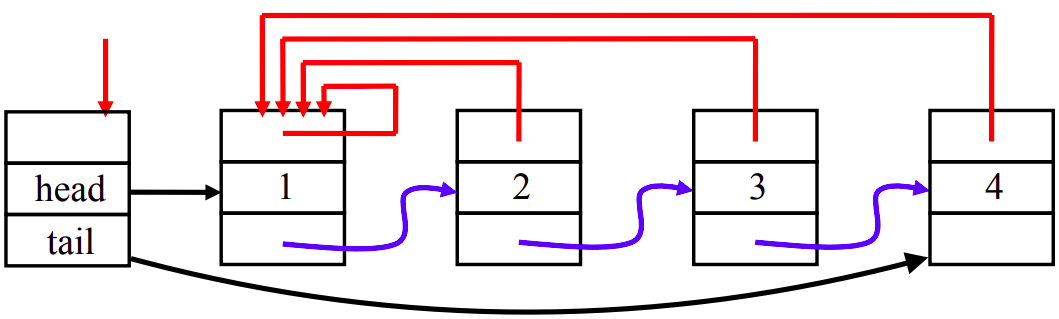
\includegraphics[width=0.8\textwidth]{merge-find-liste.png}
    \caption{\emph{Merge-find set} implementati come \emph{insiemi di liste}}
\end{figure}

\subsection{Implementazione basata su insiemi di alberi}
Ogni \emph{insieme} viene rappresentato da un \emph{albero} in cui ogni \emph{nodo}
contiene il proprio valore e un puntatore al \emph{padre}. La \emph{radice} è il
\emph{rappresentante} dell'\emph{insieme} e il puntatore al \emph{padre} punta a
se stessa.

\begin{figure}[h!]
\centering
\begin{graph}
    \node[main] (1) {$1$};
    \node[main] (2) [below left of=1, xshift=5mm, yshift=-5.8mm] {$2$};
    \node[main] (3) [below right of=1, xshift=-5mm, yshift=-5.8mm] {$3$};
    \node[main] (4) [below of=2] {$4$};

    \path[->]   (1) edge[in=75, out=105, min distance=10mm] (1)
                (2) edge (1)
                (3) edge (1)
                (4) edge (2);

    \node[main] (5) [right of=1, xshift=20mm] {$5$};
    \node[main] (6) [below of=5] {$6$};
    \node[main] (7) [below of=6] {$7$};

    \path[->]   (5) edge[in=75, out=105, min distance=10mm] (5)
                (6) edge (5)
                (7) edge (6);
\end{graph}
\caption{\emph{Merge-find set} implementati come \emph{insiemi di alberi}}
\end{figure}

\noindent
In questo caso, nel \texttt{find} si risale l'intero \emph{albero} fino alla
\emph{radice} e, nel caso pessimo, questo costa $O(n)$. Per fare la
\texttt{merge} invece, è sufficiente cambiare il puntatore al \emph{padre}
della \emph{radice} in uno dei due \emph{alberi} in modo che punti all'altra
\emph{radice}. Il costo, se non consideriamo quello per la ricerca dei
\emph{rappresentanti}, è $O(1)$.

\subsection{Implementazioni con tecniche euristiche}
Possiamo migliorare le implementazioni viste sfruttando qualche piccolo
accorgimento?

Nel caso dei \emph{merge-find set} basati su \emph{liste} potremmo provare ad
eseguire la \texttt{merge} modificando i puntatori della \emph{lista} più corta.
Per quanto riguarda gli \emph{alberi} invece, potremmo ridurre il costo della
\texttt{find} minimizzando l'\emph{altezza} degli \emph{alberi}.

Tecniche di questo tipo sono dette \emph{euristiche}, e gli algoritmi che le
usano sono detti \emph{euristici}.

\begin{definition}[Algoritmo euristico]
    È detto euristico un algoritmo progettato per risolvere un problema più
    velocemente, qualora i metodi tradizionali non siano sufficienti, oppure per
    ricavare una soluzione approssimata, qualora non sia possibile ricavarne una
    esatta.
\end{definition}

\paragraph{Euristica sul peso}
Approfondendo l'intuizione sulla lunghezza delle \emph{liste}, possiamo
memorizzare in ogni \emph{lista} l'informazione sulla propria lunghezza e
implementare la \texttt{merge} in modo che modifichi i puntatori dei \emph{nodi}
che stanno nella \emph{lista} più corta. La lunghezza può essere mantenuta in
$O(1)$ ed è possibile dimostrare che in questo tipo di implementazione il
\emph{costo ammortizzato} della \texttt{merge} è $O(\log n)$.

\paragraph{Euristica sul rango}
Abbiamo detto che per gli \emph{alberi} conviene cercare di minimizzare le
\emph{altezze}. Quindi, facciamo in modo che ogni \emph{nodo} $k$ contenga
l'informazione sul proprio \emph{rango} $rank[k]$, definito come segue:

\begin{definition}[Rango di un nodo]
    È definito rango di un nodo, il numero di archi del più lungo cammino tra
    quel nodo e una delle proprie foglie.
\end{definition}
\begin{note}
    Possiamo anche definire il \emph{rango} di un \emph{nodo} come
    l'\emph{altezza} del \emph{sottoalbero} in esso radicato.
\end{note}

\noindent
A questo punto, per ridurre il costo della \texttt{find} è sufficiente
modificare la \texttt{merge} in modo che nel caso di \emph{alberi} di con
\emph{ranghi} diversi, sia l'\emph{albero} con \emph{rango} minore ad essere
\q{agganciato} all'altro. In questa situazione, l'\emph{altezza}
dell'\emph{albero} con \emph{rango} maggiore non cambia, ma se invece i due
\emph{alberi} avessero pari \emph{rango}, l'\emph{altezza} finale sarebbe
incrementata di 1.

\bigskip\noindent
Per studiare la \emph{complessità} di questa implementazione, vediamo il
seguente teorema:

\begin{definition}[Legame tra il rango di un albero e il proprio numero di nodi]
    Un albero MFSET con radice $r$ e ottenuto tramite euristica sul rango ha
    almeno $2^{rank[r]}$ nodi.
\end{definition}
\begin{proof}[Dimostrazione]
    Procediamo per induzione sul \emph{rango} di $r$.

    \paragraph{Caso base: \bm{$rank[r]=0$}}
    Dopo l'inizializzazione della struttura ogni \emph{albero} ha $2^{rank[r]}=1$
    \emph{nodi};

    \paragraph{Passo induttivo: \bm{$rank[r]>0$}}
    Facendo la \texttt{merge} di due \emph{alberi} $x$ e $y$ di \emph{rango}
    $rank[x]$ e $rank[y]$ distinguiamo due casi:
    \begin{enumerate}
        \item \bm{$rank[x]>rank[y]$}: il \emph{rango} dell'\emph{albero} $r$
        ottenuto è $rank[r]=rank[x]$. Per induzione, il numero di \emph{nodi} di
        $r$ è almeno pari a $2{rank[x]}+2^{rank[y]}$ e quindi è maggiore di
        $2^{rank[x]}$;
        \item \bm{$rank[x]=rank[y]$}: il \emph{rango} dell'\emph{albero} $r$
        ottenuto è $rank[r]=rank[x]+1$. Per induzione, il numero di \emph{nodi}
        di $r$ è almeno pari a $2^{rank[x]}+2^{rank[y]}=2^{rank[x]}+2^{rank[x]}=
        2^{rank[x]+1}$;
    \end{enumerate}
\end{proof}

\noindent
Dal teorema appena dimostrato possiamo ricavare il seguente corollario:
\begin{definition}[Corollario]
    Un albero MFSET con radice $r$ e $n$ nodi ha un altezza inferiore a $\log n$.
\end{definition}
\begin{proof}[Dimostrazione]
    Vale la seguente relazione:
    \[n\geq 2^{rank[r]}\Leftrightarrow rank[r]\leq\log n\]
\end{proof}

\noindent
Detto questo, la \emph{complessità} della primitiva \texttt{find} è $O(\log n)$.

\paragraph{Euristica di compressione dei cammini}
Poiché il costo della \texttt{find} è legato all'\emph{altezza} degli
\emph{alberi}, se tutti avessero \emph{altezza} pari a $1$, cioè se il
\emph{padre} di ogni \emph{nodo} fosse la \emph{radice}, riusciremmo a ridurre
il costo di ogni invocazione a $O(1)$. Per raggiungere questo obiettivo, possiamo
modificare l'implementazione della \texttt{find} in modo che quando risaliamo
l'\emph{albero}, ogni \emph{nodo} modifichi il proprio puntatore al \emph{padre}
indicando il \emph{padre} del proprio \emph{padre}. In questo modo, la prima
invocazione di \texttt{find} costa $O(\log n)$, mentre ricerche successivo
su \emph{nodi} già visitati, costeranno $O(1)$.


\begin{code}{Merge-find set basati su insiemi di alberi}
\begin{minipage}[t]{0.48\textwidth}
\bc{int}[] parent\\
\bc{int}[] rank\\

\ind\bc{MFSET} Mfset(\bc{int} n)\\
    \bc{MFSET} M = new \bc{MFSET}\\
    t.parent = new \bc{int}[1\dots n]\\
    t.rank = new \bc{int}[1\dots n]\\
    \indf for (i = 1 to n) do\\
        t.parent[i] = i\\
        t.rank[i] = 1\\
    \indf return t\\

\ind\bc{int} find(\bc{int} x)\\
    \indf if (parent[x] $\neq$ x) then\\
        parent[x] = find(parent[x])\\
    \indf return parent[x]\\
\end{minipage}
\hfill
\begin{minipage}[t]{0.48\textwidth}
    \ind merge(\bc{int} x, \bc{int} y)\\
        \bc{int} r$_x$ = find(x)\\
        \bc{int} r$_y$ = find(y)\\
        \indf if (r$_x$ $\neq$ r$_y$) then\\
            \indff if (rank[r$_x$] > rank[r$_y$]) then\\
                parent[r$_y$] = r$_x$\\
            \indff else if (rank[r$_y$] > rank[r$_x$]) then\\
                parent[r$_x$] = r$_y$\\
            \indff else\\
                parent[r$_x$] = r$_y$\\
                rank[r$_y$] = rank[r$_y$] + 1\\
\end{minipage}
\end{code}
\chapter{Programmazione dinamica}
\section{Introduzione}
Finora, l'unica tecnica di risoluzione di problemi, o di ricerca di algoritmi,
che abbiamo visto è il \nameref{chap:divide-et-impera}. La \emph{programmazione
dinamica} è un'altra tecnica basata su un approccio molto simile.

Entrambe prevedono di spezzare il problema di partenza in sotto-problemi più
semplici e di ricostruire la soluzione del problema originale a partire dalle
soluzioni dei sotto-problemi. La differenza fondamentale sta nel fatto che la
\emph{programmazione dinamica} risolve ogni sotto-problema una sola volta,
mentre il \emph{Divide-et-impera} non pone questo vincolo.

Per realizzare ciò, le soluzioni di tutti i sotto-problemi vengono salvate in
una tabella che viene consultata ogni volta che è necessario risolvere uno
dei sotto-problemi. In particolare, se la tabella non contiene la soluzione
al sotto-problema considerato, questa viene calcolata e aggiunta alla tabella.
In caso contrario, viene sfruttata la soluzione già nota.

\subsection{Approccio generale}
\begin{figure}[hb!]
    \centering
    \scalebox{0.83}{
        \begin{graph}
            \tikzset{rect/.style={draw, rectangle, minimum size=15mm,
                rounded corners=0.25cm, inner sep=5mm}}
            \node[rect] (1) {Problema di ottimizzazione};
    
            \node[rect] (2) [below of=1, yshift=-7.5mm] {\shortstack{Definizione della soluzione\\in maniera ricorsiva}};
            \node[rect] (3) [right of=2, xshift=100mm] {\shortstack{Definizione del valore della\\soluzione in maniera ricorsiva}};
            \node[rect] (4) [above of=3, yshift=7.5mm] {Problema di conteggio};
    
            \node[rect] (5) [below of=3, xshift=-120mm, yshift=-15mm]
                {\emph{Divide-et-impera}};
            \node[rect] (6) [below of=3, xshift=-60mm, yshift=-15mm]
                {\emph{\shortstack{Programmazione\\dinamica}}};
            \node[rect] (7) [below of=3, xshift=0mm, yshift=-15mm]
                {\emph{Memoization}};
    
            \node[rect] (8) [below of=7, yshift=-7.5mm, xshift=-27.5mm]
                {Tabella delle soluzioni};

            \node[rect] (9) [right of=8, xshift=30mm] {\shortstack{Output\\numerico}};
            \node[rect] (10) [left of=8, xshift=-40mm]
                {\shortstack{Ricostruzione\\della soluzione}};
            \node[rect] (11) [left of=10, xshift=-30mm] {\shortstack{Soluzione\\ottima}};
    
            \path[->]   (1) edge (2)
                        (2) edge (3)
                        (4) edge (3)
                        (3.west)+(0mm, -2mm)
                            edge [bend right=15]
                            node [near end, left]
                                {\shortstack{Non ci sono sotto-problemi\\ripetuti}}
                        (5.north)
                        (3)
                            edge [bend right=5]
                            node [midway, left=2mm]
                                {\shortstack{Ci sono sotto-problemi\\ripetuti e devono essere\\ risolti tutti}}
                        (6)
                        (3)
                            edge [bend left=10]
                            node [midway, right]
                                {\shortstack{Ci sono sotto-problemi\\ripetuti, ma ne devono\\essere risolti solo\\alcuni}}
                        (7.north)
                        (6.south east)+(-1mm, 1mm) edge [bend left=15] (8)
                        (7.south west)+(1mm, 1mm) edge [bend right=15] (8)
                        (8) edge (9)
                        (8) edge (10)
                        (10) edge (11);
        \end{graph}
    }
    \caption{Schema generale di approccio}
\end{figure}\noindent
Lo schema di cui sopra mostra un approccio generale alla scelta della tecnica
risolutiva più adatta al tipo di problema da risolvere. In particolare,
distinguiamo la soluzione del problema dal proprio valore, ad esempio, nella
ricerca del \emph{cammino breve} tra due \emph{nodi}, la soluzione è il
\emph{cammino}, mentre il valore potrebbe esserne la lunghezza.

Una volta definiti questi parametri, se la suddivisione del problema non
porta a dover risolvere più volte uno stesso sotto-problema, possiamo procedere
ad implementare la soluzione sfruttando l'approccio \emph{Divide-et-impera}
classico. Caso contrario, ricadiamo nei casi d'uso della \emph{programmazione
dinamica}, ma dobbiamo ancora fare una distinzione: la risoluzione di alcuni dei
sotto-problemi potrebbe non essere necessaria per arrivare alla soluzione del
problema di partenza. Se il caso è questo, procediamo con la tecnica della
\emph{memoization} che non è altro se non un approccio top-down alla
\emph{programmazione dinamica} \q{classica}.

In ogni caso, utilizzando la \emph{programmazione dinamica} si arriva alla
definizione di una \emph{tabella delle soluzioni} e, se il problema è un
\emph{problema di conteggio}, da cui possiamo ricavare direttamente la soluzione.
Se invece stiamo considerando un \emph{problema di ottimizzazione}, la
soluzione dovrà essere ricavata attraverso un processo di \q{ricostruzione}.

\section{Gioco del domino}
Vediamo adesso un primo esempio di utilizzo della \emph{programmazione dinamica}
e di come la soluzione si differenzi, soprattutto in termini di efficienza, da
una classica soluzione \emph{divide-et-impera}.

\begin{problem}[Domino lineare]
    Il gioco del domino è basato su tessere di dimensione $2\times1$. Scrivere un
    algoritmo che prenda in input un valore intero positivo $n$ e restituisca il
    numero di modi in cui è possibile disporre le tessere del gioco in modo che
    creino un rettangolo $2\times n$.
\end{problem}\noindent
Ad esempio, per $n$ pari a 0, 1, 2, 3, 4 l'algoritmo dovrà restituire 1, 1,
2, 3, 5.
\begin{note}
    Per $n=0$, restituiamo 1 perché per ottenere un rettangolo di dimensione
    $2\times 0$ c'è un solo modo: non disporre nessuna tessera.
\end{note}\noindent
Basandoci sullo schema di cui sopra possiamo identificare questo problema con
un \emph{problema di conteggio} e quindi la prima cosa da fare è la \q{definizione
del valore della soluzione in maniera ricorsiva}.

\subsection{Approccio basato su divide-et-impera}

Chiamiamo $DP[n]$ la funzione che per ogni valore $n\in\mathbb{N}$ restituisce il
numero di disposizioni possibili delle tessere. La funzione $DP$ è ricorsiva, quindi,
prima di tutto identifichiamo il caso base: poiché per $n=0$ e $n=1$ $DP[n]=1$,
possiamo decidere che $DP[n]=1$ per $n\leq1$.

A questo punto, consideriamo il caso più complesso in cui dobbiamo esaminare un
rettangolo $2\times n$ arbitrariamente grande. Poiché le tessere del domino hanno
dimensione $2\times1$ e non posso essere posizionate in modo sfalsato, i
possibili posizionamenti di ogni tessera sono due: in verticale o in orizzontale.
Se ipotizzassimo di mettere una tessera verticale a destra o a sinistra del
rettangolo, il problema si ridurrebbe all'analisi di un rettangolo $2\times(n-1)$.
Se invece posizionassimo la tessera in orizzontale otterremmo una figura composta
da un rettangolo $2\times(n-2)$ e da un altro rettangolo più piccolo di
dimensione $1\times2$. Chiaramente, il rettangolo più piccolo corrisponde ad una
tessera orizzontale posta sopra o sotto quella che abbiamo già messo e, di
conseguenza, arriviamo alla conclusione che qual'ora si disponga una tessera in
orizzontale se ne debba sempre aggiungere anche una seconda sopra o sotto la prima.

\noindent
Fatta questa riflessione possiamo terminare dicendo che, dato un
generico rettangolo $2\times n$, il numero di possibili disposizioni di tessere
è pari a $DP[n-1]+DP[n-2]$ e che quindi la definizione della funzione ricorsiva
è:
\[DP[n]=\begin{cases}
    1 & n\leq1\\
    DP[n-1]+DP[n-2] & n>1
\end{cases}\]
\begin{note}
    Le soluzioni per $n-1$ e $n-2$ si sommano perché per ogni rettangolo $2\times
    n$ ho la possibilità di mettere una tessera verticale o due tessere orizzontali.
\end{note}

\bigskip\noindent
Provando a valutare la funzione per valori crescenti di $n$ otteniamo la
seguente sequenza:
\[1,1,2,3,5,8,13,21,34,55,89,\dots\]
che corrisponde esattamente alla \emph{sequenza di Fibonacci}. L'implementazione
dell'algoritmo corrisponde perciò all'implementazione della funzione per il
calcolo di tale sequenza.

\begin{minicode}{Prima implementazione della soluzione}
    \ind\bc{int} domino1(\bc{int} n)\\
        \indf if (n $\leq$ 1) then\\
            return 1\\
        \indf else\\
            return domino1(n-1) + domino1(n-2)
\end{minicode}\noindent
La \emph{funzione di ricorrenza} associata a questa funzione è la seguente:
\[T(n)=\begin{cases}
    1 & n\leq1\\
    T(n-1)+T(n-2) & n>1
\end{cases}\]
Per il \emph{\nameref{def:21}} la \emph{forma chiusa} di tale funzione è
$T(n)=\Theta(2^n)$. Un costo esponenziale è tutt'altro che efficiente, non
possiamo fare meglio di così?

\bigskip\noindent Proviamo ad esaminare l'\emph{albero delle invocazioni} per
$n=6$:

\begin{figure*}[h!]
\centering
\resizebox*{\linewidth}{!}{
\begin{graph}
    \node[main] (6-1)   {$6$};
    \node[main] (5-2)   [below left of=6-1, xshift=-35mm] {$5$};
    \node[main] (4-2)   [below right of=6-1, xshift=35mm] {$4$};

    \node[main] (4-3)   [below left of=5-2, xshift=-12.5mm] {$4$};
    \node[main] (3-3)   [below right of=5-2, xshift=12.5mm] {$3$};
    \node[main] (3-3d)  [below left of=4-2, xshift=-12.5mm] {$3$};
    \node[main] (2-3)   [below right of=4-2, xshift=12.5mm] {$2$};

    \node[main] (3-4)   [below left of=4-3] {$3$};
    \node[main] (2-4)   [below right of=4-3] {$2$};
    \node[main] (2-4d)  [below left of=3-3] {$2$};
    \node[main] (1-4)   [below right of=3-3] {$1$};
    \node[main] (2-4dd)   [below left of=3-3d] {$2$};
    \node[main] (1-4d)   [below right of=3-3d] {$1$};
    \node[main] (1-4dd)  [below left of=2-3] {$1$};
    \node[main] (0-4)   [below right of=2-3] {$0$};

    \node[main] (2-5)   [below of=3-4, xshift=-20] {$2$};
    \node[main] (1-5)   [below of=3-4, xshift=20] {$1$};
    \node[main] (1-5d)  [below of=2-4, xshift=-20] {$1$};
    \node[main] (0-5)  [below of=2-4, xshift=20] {$0$};
    \node[main] (1-5dd)  [below of=2-4d, xshift=-20] {$1$};
    \node[main] (0-5d)  [below of=2-4d, xshift=20] {$0$};
    \node[main] (1-5ddd)  [below of=2-4dd, xshift=-20] {$1$};
    \node[main] (0-5dd)  [below of=2-4dd, xshift=20] {$0$};

    \node[main] (1-6) [below of=2-5, xshift=-15] {$1$};
    \node[main] (0-6) [below of=2-5, xshift=15] {$0$};

    \path[-]    (6-1) edge (5-2)
                (6-1) edge (4-2)
                (5-2) edge (4-3)
                (5-2) edge (3-3)
                (4-2) edge (3-3d)
                (4-2) edge (2-3)
                (4-3) edge (3-4)
                (4-3) edge (2-4)
                (3-3) edge (2-4d)
                (3-3) edge (1-4)
                (3-3d) edge (2-4dd)
                (3-3d) edge (1-4d)
                (2-3) edge (1-4dd)
                (2-3) edge (0-4)
                (3-4) edge (2-5)
                (3-4) edge (1-5)
                (2-4) edge (1-5d)
                (2-4) edge (0-5)
                (2-4d) edge (1-5dd)
                (2-4d) edge (0-5d)
                (2-4dd) edge (1-5ddd)
                (2-4dd) edge (0-5dd)
                (2-5) edge (1-6)
                (2-5) edge (0-6);
\end{graph}
}
\end{figure*}\noindent
Se ogni \emph{nodo} rappresenta un sotto-problema, è evidente come molti
sotto-problemi vengano risolti più di una volta. Questa è sicuramente
un'inefficienza, quindi, proviamo ad evitare di eseguire invocazioni ridondanti.

\subsection{Approccio basato su programmazione dinamica}
La presenza di sotto-problemi ripetuti ci costringe quindi ad evitare una
soluzione realizzata con un classico \emph{divide-et-impera}, e ad utilizzare
invece la \emph{programmazione dinamica}, con conseguente costruzione di una
\emph{tabella delle soluzioni}. In particolare, tale tabella conterrà un elemento
per ogni sotto-problema da risolvere.

Poiché, per ogni $n\in\mathbb{N}$ il calcolo della soluzione si basa su i due
valori precedenti di $n$, ci troviamo in una situazione in cui tutti i
sotto-problemi devono essere risolti e quindi procediamo con la
\emph{programmazione dinamica} classica o bottom-up. Ciò significa che per
costruire la \emph{tabella delle soluzioni} partiamo dai casi base e risaliamo
fino ad $n$.

\begin{minicode}{Seconda implementazione della soluzione}
    \ind\bc{int} domino2(\bc{int} n)\\
        \bc{int}[] DP = new \bc{int}[0\dots n]\hfill\com{\emph{Tabella delle soluzioni}}
        DP[0] = 1\\
        DP[1] = 1\\
        \indf for (i = 2 to n) do\\
            DP[i] = DP[i - 1] + DP[i - 2]\\
        \indf return DP[n]
\end{minicode}
\begin{note}
    Sebbene finora avessimo parlato soltanto di soluzioni ricorsive, nulla ci
    vieta di realizzarne di iterative se queste sono estensionalmente equivalenti.
\end{note}\noindent
L'aumento in efficienza è evidente in quanto la \emph{complessità} si è ridotta
a $\Theta(n)$, tuttavia, l'utilizzo di una \emph{tabella delle soluzioni} ci
porta a considerare anche la \emph{complessità} dal punto di vista spaziale, cioè
quanto spazio di memoria è necessario per la sua memorizzazione. In questo caso
memorizziamo i valori in un vettore di dimensione $n+1$, quindi la
\emph{complessità} è $S(n)=\Theta(n)$.

\bigskip\noindent Possiamo fare meglio di così?

Da un punto di vista temporale no, ma da quello spaziale si. Se consideriamo bene
la funzione ci rendiamo facilmente conto del fatto che, ad ogni iterazione,
utilizziamo soltanto i valori delle due posizioni precedenti. Di conseguenza,
potremmo eliminare il vettore e utilizzare delle semplici variabili.

\begin{minicode}{Terza implementazione della soluzione}
    \ind\bc{int} domino3(\bc{int} n)\\
        \bc{int} DP$_0$ = 1\\
        \bc{int} DP$_1$ = 1\\
        \bc{int} DP$_2$ = 1\\
        \indf for (i = 2 to n) do\\
            DP$_0$ = DP$_1$\\
            DP$_1$ = DP$_2$\\
            DP$_2$ = DP$_1$ + DP$_0$\\
        \indf return DP$_2$
\end{minicode}\noindent
Ora, la \emph{complessità spaziale} si è ridotta a $\Theta(1)$.

\paragraph{Criterio di costo logaritmico}
Le \emph{complessità} calcolate finora sono tali fino a quando ci basiamo su
un \emph{criterio di costo uniforme}, nel quale consideriamo soltanto il
numero di elementi. Ora però, proviamo a chiederci come cambierebbero le
\emph{complessità} se utilizzassimo un \emph{criterio di costo logaritmico}.

\noindent
Iniziamo ragionando sul modo in cui crescono i numeri della serie di Fibonacci.
Se $F(n)$ è l'$n$-esimo numero della serie, vale la \emph{formula di Binet}:
\[F(n)=\frac{\phi^n}{\sqrt{5}}-\frac{(1-\phi)^n}{\sqrt{5}}\quad\text{con}
\quad\phi=\frac{1+\sqrt{5}}{2}=1.6180339887\dots\footnotemark\]
\begin{note}
    Vale la pena far notare che $F(n)=DP[n-1]$ perché $DP$ vale per $n\geq0$,
    mentre $F(n)$ per $n\geq1$.
\end{note}\noindent
Il primo termine della formula è un'esponenziale con base un numero maggiore di $1$,
quindi cresce esponenzialmente, mentre il secondo tende a $0$. Questo ci dice
che i bit necessari a memorizzare l'$n$-esimo valore della serie crescono
linearmente. Ovvero, per memorizzare l'$n$-esimo termine servono $\Theta(n)$ bit
e sommare due valori consecutivi costa $\Theta(n)$.

\footnotetext{$\phi$ rappresenta il valore della \emph{sezione aurea} ed è
anche definito come $\lim_{n\to+\infty}\frac{F(n+1)}{F(n)}$, ovvero come
il rapporto tra numeri consecutivi della serie di Fibonacci}

Detto questo, possiamo ricalcolare tutte le \emph{complessità} delle tre soluzioni
sotto il \emph{criterio di costo logaritmico}.

\begin{table}[h!]
    \centering
    \renewcommand{\arraystretch}{1.2}
    \begin{tabular}{|c|c|c|}
        \hline
        \textbf{Soluzione} & \textbf{Complessità temporale} & \textbf{Complessità
        spaziale} \\
        \hline
        \texttt{domino1} & $O(n2^n)$ & $O(n^2)$\\
        \hline
        \texttt{domino2} & $O(n^2)$ & $O(n^2)$\\
        \hline
        \texttt{domino3} & $O(n^2)$ & $O(n)$\\
        \hline
    \end{tabular}
\end{table}
\begin{note}
    In pratica, abbiamo semplicemente moltiplicato per $n$ tutti i valori.
\end{note}

\section{Problema di Hateville}
\begin{problem}[Hateville]
    Hateville è un villaggio particolare composto da $n$ case numerate e
    disposte linearmente lungo una singola strada. Ad Hateville ognuno odia i
    propri vicini: l'abitante $i$ odia i suoi vicini $i-1$ e $i+1$ (se esistono).

    Si vuole realizzare una sagra per la quale è necessario raccogliere dei fondi.
    Ogni abitante $i$ è disposto a donare una quantità $D[i]$, ma solo se nessuno
    dei suoi vicini partecipa.

    Scrivere un algoritmo che restituisca la quantità massima di fondi che può
    essere raccolta e un secondo algoritmo che restituisca il sottoinsieme di
    indici $S\subseteq\{1,\dots,n\}$ tale per cui la donazione totale $T=\sum_{i
    \in S}D[i]$ sia massimale.
\end{problem}\noindent
Ad esempio, se il vettore delle donazioni è $D=[10,5,5,10]$ la massima quantità
di fondi che può essere raccolta è $20$ e l'insieme $S$ è $\{1,4\}$.

\subsection{Approccio basato su divide-et-impera}
Iniziamo provando a ridefinire il problema. Se $HV(i)$ è uno dei possibili
insiemi di indici che consente di ottenere una raccolta massimale dalle prime
$i$ case, la soluzione al problema è $HV(n)$.

Consideriamo ora il vicino $i$. Possiamo accettare o meno la sua donazione.
Se non la accettiamo possiamo accettare quella del vicino $i-1$ e quindi
$HV(i)=HV(i-1)$. Se invece accettiamo la donazione di $i$, dobbiamo rifiutare
quella di $i-1$, perciò $HV(i)=HV(i-2)\cup\{i\}$.

\noindent
Per decidere se accettare o meno la donazione di $i$ è sufficiente vedere
quale scelta permette di raccogliere più fondi. Se $highest$ è una
funzione che, dati due insiemi, seleziona quello che garantisce una donazione
più alta, $HV(i)$ diventa:
\[HV(i)=highest\left(HV(i-1),HV(i-2)\cup\{i\}\right)\]
Ciò che abbiamo detto finora è vero secondo quanto affermato dal seguente teorema:
\begin{definition}[Sottostruttura ottima]
    Siano $P_i$ il problema dato dalle prime $i$ case e $S_i$ una sua soluzione
    ottima. Valgono le seguenti:
    \begin{enumerate}
        \item Se $i\notin S_i$, allora $S_i=S_{i-1}$;
        \item Se $i\in S_i$, allora $S_i=S_{i-2}\cup\{i\}$;
    \end{enumerate}
\end{definition}

\begin{proof}[Dimostrazione]
    Procediamo dimostrando separatamente i due punti.
    \paragraph{Caso 1: \bm{$i\notin S_i$}}
    Secondo il teorema, $S_i=S_{i-1}$, cioè $S_i$ è la soluzione ottima sia di
    $P_i$ che di $P_{i-1}$. Se supponessimo, per assurdo, che non fosse così,
    dovrebbe esistere una soluzione $S'_{i-1}$ per il problema $P_{i-1}$ tale
    che $S'_{i-1}=highest\left(S'_{i-1}, S_i\right)$. Cioè, la soluzione $S'_{i-1}$
    dovrebbe garantire una donazione maggiore di quella di $S_i$. Ma, se fosse
    così, $S'_{i-1}$ dovrebbe essere anche la soluzione di $P_i$, generando un
    assurdo.

    \paragraph{Caso 2: \bm{$i\in S_i$}}
    Se $i\in S_i$, $i-1\notin S_i$, altrimenti non sarebbe una soluzione
    ammissibile. Quindi, $S_i-\{i\}$ deve essere una soluzione ottima per
    $P_{i-2}$. Se supponessimo, per assurdo, che non fosse così, dovrebbe
    esistere una soluzione $S'_{i-2}$ per il problema $P_{i-2}$ tale che
    $S'_{i-2}=highest\left(S'_{i-2}, S_i-\{i\}\right)$. Ma, se fosse così,
    $S'_{i-2}\cup\{i\}$ dovrebbe essere una soluzione di $P_i$ migliore di
    $S_i$, generando un assurdo.
\end{proof}\noindent
Dimostrate le nostre ipotesi, possiamo procedere con la definizione ricorsiva
della soluzione. I casi base sono due:
\begin{itemize}
    \item Se $i=0$, $HV(0)=\emptyset$;
    \item Se $i=1$, $HV(1)=\{1\}$;
\end{itemize}
La funzione che otteniamo è la seguente:
\[HV(i)=\begin{cases}
    \emptyset & i=0\\
    \{1\} & i=1\\
    highest\left(HV(i-1), HV(i-2)\cup\{i\}\right) & i\geq2
\end{cases}\]
Osservando la definizione possiamo notare la similitudine con la funzione per il
calcolo della \emph{sequenza di Fibonacci}. Essendoci sotto-problemi ripetuti,
possiamo scartare subito qualunque soluzione basata su \emph{divide-et-impera}.

\subsection{Approccio basato su programmazione dinamica}
La \emph{programmazione dinamica} ci richiede di costruire una \emph{tabella
delle soluzioni}. Proviamo a costruire tale tabella partendo da un esempio:
sia il vettore delle donazioni $D$ definito come segue:
\[D=[10,5,5,8,4,7,12]\]

\newpage\noindent
La \emph{tabella delle soluzioni} è la seguente:

\begin{table}[ht!]
    \centering
    \renewcommand{\arraystretch}{1.2}
    \begin{tabular}{|c|c|c|c|c|c|c|c|c|}
        \hline
        \bm{$i$} & \bm{$0$} & \bm{$1$} & \bm{$2$} & \bm{$3$} & \bm{$4$} & 
        \bm{$5$} & \bm{$6$} & \bm{$7$}\\
        \hline
        $HV$ & $\emptyset$ & $\{1\}$ & $\{1\}$ & $\{1,3\}$ & $\{1,4\}$ &
        $\{1,3,5\}$ & $\{1,4,6\}$ & $\{1,3,5,7\}$\\
        \hline
    \end{tabular}
\end{table}\noindent
Ci sono un paio di problemi. Prima di tutto dobbiamo definire la funzione
$highest$, ma il problema più grosso è la difficoltà di memorizzazione degli
insiemi in una tabella.

Per risolvere entrambi i problemi in una volta potremmo definire il valore delle
soluzioni come la quantità di fondi che vengono raccolti. Definiamo quindi una
funzione $DP$ tale che $DP[i]$ è la massima quantità di fondi che si possono
ottenere dalle prime $i$ case di Hateville. Partendo da $HV$ possiamo definire
$DP$ come segue:
\[DP[i]=\begin{cases}
    0 & i=0\\
    D[1] & i=1\\
    \max\left(DP[i-1], DP[i-2]+D[i]\right) & i\geq2
\end{cases}\]\noindent
Adesso implementare la soluzione è una banalità.

\begin{minicode}{Implementazione della soluzione al primo problema}
\ind\bc{int} hateville(\bc{int}[] D, \bc{int} n)\\
    \bc{int}[] DP = new \bc{int}[0\dots n]\hfill\com{\emph{Tabella delle soluzioni}}
    DP[0] = 0\\
    DP[1] = D[1]\\
    \indf for (i = 2 to n) do\\
        DP[i] = max(DP[i - 1], DP[i - 2] + D[i])\\
    \indf return DP[n]
\end{minicode}\noindent
La \emph{complessità temporale} e \emph{spaziale} della soluzione sono entrambe
$\Theta(n)$. Possiamo notare che, come nel problema del domino, per ogni $i$ la
soluzione è ottenuta a partire dalle soluzioni dei due valori precedenti di $i$,
quindi, potremmo eliminare l'array e introdurre delle variabili semplici
riducendo a $\Theta(1)$ la \emph{complessità spaziale}.

\begin{minicode}{Implementazione migliorata della soluzione al primo problema}
\ind\bc{int} hateville(\bc{int}[] D, \bc{int} n)\\
    \bc{int} DP$_0$ = 0\\
    \bc{int} DP$_1$ = 1\\
    \bc{int} DP$_2$ = 1\\
    \indf for (i = 2 to n) do\\
        DP$_2$ = max(DP$_1$, DP$_0$ + D[i])\\
    \indf return DP$_2$
\end{minicode}

\paragraph{Ricostruire la soluzione}
A questo punto abbiamo risolto la prima richiesta del problema. Per quanto
riguarda la seconda, dobbiamo riuscire a ricostruire l'insieme di indici a
partire dalla \emph{tabella delle soluzioni}. Grazie al teorema sulla
\emph{\nameref{def:107}} possiamo fare le seguenti assunzioni:
\begin{itemize}
    \item Se la casa $i$ non è stata selezionata, $i\notin S_i$ e quindi $S_i=S_
    {i-1}$. Questo, riflesso sulla \emph{tabella delle soluzioni}, garantisce che
    se $DP[i]=DP[i-1]$, $i$ non appartiene all'insieme $S$ di indici;
    \item Se la casa $i$ è stata selezionata, $i\in S_i$ e quindi $S_i=S_{i-2}
    \cup\{i\}$. Questo, riflesso sulla \emph{tabella delle soluzioni}, garantisce
    che se $DP[i]=DP[i-2]+D[i]$, $i$ appartiene all'insieme $S$ di indici;
\end{itemize}
\begin{note}
    È possibile che risultino verificati entrambi i casi e, se succede, significa
    che esistono due soluzioni possibili.
\end{note}\noindent
Chiariti questi punti, possiamo ricostruire la soluzione fino a $i$ in modo
ricorsivo. Nello specifico, se $DP[i]=DP[i-1]$, si prende la soluzione valida per
$i-1$, altrimenti si prende quella valida per $i-2$ e le si aggiunge $i$.

\begin{minicode}{Implementazione della soluzione al secondo problema}
\ind\bc{SET} hateville(\bc{int}[] D, \bc{int} n)\\
    \bc{int}[] DP = new \bc{int}[0\dots n]\hfill\com{\emph{Tabella delle soluzioni}}
    DP[0] = 0\\
    DP[1] = D[1]\\
    \indf for (i = 2 to n) do\\
        DP[i] = max(DP[i - 1], DP[i - 2] + D[i])\\
    \indf return solution(DP, n)\\

\com{Funzione ausiliaria per la ricostruzione della soluzione}
\rmindent\ind\bc{SET} solution(\bc{int}[] DP, \bc{int} i)\\
    \indf if (i == 0) then\\
        return $\emptyset$\\
    \indf if (i == 1) then\\
        return \{1\}\\
    \indf if (DP[i] == DP[i - 1]) then\\
        return solution(DP, i - 1)\\
    \indf else\\
        \bc{SET} sol = solution(DP, i - 2)\\
        sol.insert(i)\\
        return sol\\
\end{minicode}\noindent
La \emph{complessità temporale} di \texttt{solution} è $\Theta(n)$.
\begin{note}
    È importante notare che non avremmo potuto ricostruire la soluzione senza
    l'intera \emph{tabella delle soluzioni} e quindi non possiamo utilizzare
    la versione migliorata di \texttt{hateville}.
\end{note}

\section{Problema dello zaino}
\begin{problem}[Problema dello zaino\footnotemark]
    Dato un insieme di oggetti, ognuno caratterizzato da un peso e da un profitto,
    e uno \q{zaino} di capacità finita, individuare un sottoinsieme di oggetti
    tali per cui il loro peso totale sia al più uguale alla capacità dello zaino
    e il loro profitto totale sia massimale.
\end{problem}

\footnotetext{Questo è uno dei problemi classici dell'informatica ed è noto
con il nome di \emph{Knapsack problem}}\noindent
Questo problema ci chiede di realizzare un algoritmo che prenda in input un
vettore $w$ dei pesi, un vettore $p$ dei profitti e la capacità $C$ dello zaino
e che restituisca un insieme $S\subseteq\{1,\dots,n\}$ tale che:
\begin{itemize}
    \item il peso totale non superi la capacità, cioè $w(S)=\sum_{i\in S}w[i]
    \leq C$;
    \item il profitto totale sia massimale, cioè $argmax_S\ p[S]=\sum_{i\in S}
    p[i]$;
\end{itemize}
Ad esempio, se $C=12$, $w=[10,4,8]$ e $p=[20,6,12]$, l'algoritmo deve
restituire l'insieme $S=\{1\}$.

\bigskip\noindent
Proviamo a dare un valore alla soluzione. Definiamo una funzione $DP[i][c]$ come
il massimo profitto che può essere ottenuto dai primi $0\leq i\leq n$ oggetti
in uno zaino di capacità $c\leq C$. Il massimo profitto ottenibile nel problema
originale è allora $DP[n][C]$.

Ora, consideriamo un generico oggetto $i$. Se non lo prendiamo, $DP[i][c]=
DP[i-1][c]$ perché non cambiano né il profitto né la capacità. Se invece lo
prendiamo, $DP[i][c]=DP[i-1][c-w[i]]+p[i]$ in quanto, il peso dell'oggetto $i$
viene sottratto alla capacità rimanente e il profitto associato viene aggiunto
a quello ottenuto con i precedenti $i-1$ oggetti.

La scelta migliore tra le due è quella che massimizza il profitto e la possiamo
sintetizzare con la seguente:
\[DP[i][c]=\max\left(\overbrace{DP[i-1][c-w[i]]+p[i]}^{\text{Preso}},\;
\overbrace{DP[i-1][c]}^{\text{Non preso}}\right)\]
Per quanto riguarda i casi base, è facile dedurre che per $i=0$ o $c=0$, il
profitto massimo possibile sia $0$. C'è però un terzo caso: quando proviamo a
prendere un oggetto, lo facciamo senza verificare che il peso non superi la
capacità, quindi, potremmo ritrovarci ad avere un valore negativo per quest'ultima.
Se questo succede, è ovvio che non avremmo potuto raccogliere quell'oggetto e,
di conseguenza, decidiamo che in quel caso il profitto valga $-\infty$ in modo da
assicurare che non venga selezionato dalla funzione $\max$.

Detto questo, possiamo scrivere la formula nella sua forma completa:
\[DP[i][c]=\begin{cases}
    0 & i=0 \vee c=0\\
    -\infty & c<0\\
    \max\left(DP[i-1][c-w[i]]+p[i],\; DP[i-1][c]\right) & \text{altrimenti}
\end{cases}\]
Equivalentemente, possiamo rimuovere il $-\infty$ e riscrivere la formula come
segue:
\[DP[i][c]=\begin{cases}
    0 & i=0 \vee c=0\\
    DP[i-1][c] & w[i]>c\\
    \max\left(DP[i-1][c-w[i]]+p[i],\; DP[i-1][c]\right) & w[i]\leq c
\end{cases}\]

\subsection{Approccio basato su programmazione dinamica}
\begin{minicode}{Implementazione iterativa della soluzione}
\ind\bc{int} knapsack(\bc{int}[] w, \bc{int}[] p, \bc{int} n, \bc{int} C)\\
    \bc{int}[][] DP = new \bc{int}[0\dots n][0\dots C]\hfill\com{\emph{Tabella
    delle soluzioni}}
    \indf for (i = 0 to n) do\\
        DP[i][0] = 0\\
    \indf for (c = 0 to C) do\\
        DP[0][c] = 0\\
    \indf for (i = 1 to n) do\\
        \indff for (c = 1 to C) do\\
            \indfff if (w[i] $\leq$ c) then\\
                DP[i][c] = max(DP[i - 1][c - w[i]] + p[i], DP[i - 1][c])\\
\end{minicode}
\begin{codecont}
    \indff else\\
        \indfff DP[i][c] = DP[i - 1][c]\\
    \rmindent return DP[n][C]
\end{codecont}

\begin{eg}[Esempio di esecuzione]
    Dato uno zaino di capacità $C=9$ e i seguenti vettori dei pesi e dei
    profitti:
    \[w=[4,2,3,4]\]
    \[p=[10,7,8,6]\]
    al termine dell'esecuzione dell'algoritmo di cui sopra, la matrice $DP$
    corrisponde alla seguente tabella:

    \begin{table}[h!]
        \renewcommand{\arraystretch}{1.2}
        \centering
        \begin{tabular}{|c|c|c|c|c|c|c|c|c|c|c|}
            \hline
             & \multicolumn{10}{c|}{\bm{$c$}}\\
            \hline
            \bm{$i$} & \bm{$0$} & \bm{$1$} & \bm{$2$} & \bm{$3$} & \bm{$4$} &
            \bm{$5$} & \bm{$6$} & \bm{$7$} & \bm{$8$} & \bm{$9$}\\
            \hline
            \bm{$0$} & 0 & 0 & 0 & 0 & 0 & 0 & 0 & 0 & 0 & 0\\
            \hline
            \bm{$1$} & 0 & 0 & 0 & 0 & 10 & 10 & 10 & 10 & 10 & 10\\
            \hline
            \bm{$2$} & 0 & 0 & 7 & 7 & 10 & 10 & 17 & 17 & 17 & 17\\
            \hline
            \bm{$3$} & 0 & 0 & 7 & 8 & 10 & 15 & 17 & 18 & 18 & 25\\
            \hline
            \bm{$4$} & 0 & 0 & 7 & 8 & 10 & 15 & 17 & 18 & 18 & 25\\
            \hline
        \end{tabular}
    \end{table}
\end{eg}

\paragraph{Complessità}
Siccome l'algoritmo costruisce e popola una tabella di dimensione $n\cdot C$,
la \emph{complessità} è $T(n)=\Theta(nC)$. Ovviamente lo stesso vale anche per 
la \emph{complessità spaziale}. Quindi, il costo dell'algoritmo dipende da due
variabili, ma poiché $C$ non rappresenta la dimensione dell'input e viene
rappresentato mediante $k=\lceil\log C\rceil$ bit, la \emph{complessità
temporale} può essere riscritta come:
\[T(n)=\Theta(n2^k)\]
Ciò, rende questa implementazione dell'algoritmo \emph{pseudo-polinomiale}\footnotemark.

\footnotetext{Parleremo meglio di cosa significhi più avanti nella trattazione}

\bigskip\noindent
È possibile fare meglio di così?

Possiamo provare a realizzare una versione ricorsiva dell'algoritmo.

\begin{minicode}{Implementazione ricorsiva della soluzione}
\ind\bc{int} knapsack(\bc{int}[] w, \bc{int}[] p, \bc{int} n, \bc{C})\\
    return knapsackRec(w, p, n, C)\\

\ind\bc{int} knapsackRec(\bc{int}[] w, \bc{int}[] p, \bc{int} n, \bc{c})\\
    \indf if (c $\leq$ 0) then\\
        return -$\infty$\\
    \indf if (i == 0 or c == 0) then\\
        return 0\\
    \indf\bc{int} notTaken = knapsackRec(w, p, i - 1, c)\\
    \indf\bc{int} taken = knapsackRec(w, p, i - 1, c - w[i]) + p[i]\\
    \indf return max(notTaken, taken)
\end{minicode}\noindent
In questa implementazione abbiamo semplicemente tradotto in codice la prima
forma della formula per $DP$ e l'\emph{equazione di ricorrenza} è:
\[T(n)=\begin{cases}
    1 & n\leq1\\
    2T(n-1)+1 & n>1
\end{cases}\]
Per il \emph{\nameref{def:21}} la \emph{forma chiusa} associata è
$T(n)=\Theta(2^n)$ e quindi la \emph{complessità} è addirittura più alta di
quella della soluzione iterativa.

Purtroppo infatti, secondo l'opinione della maggior parte degli informatici,
non esistono soluzioni meno complesse di quelle che abbiamo esaminato. Ciò
che possiamo comunque provare a fare, è realizzare delle implementazioni che,
a parità di \emph{complessità}, migliorino quelle già esistenti.

\subsection{Approccio basato su memoization}
Come già accennato, la \emph{memoization} è una tecnica risolutiva che unisce
l'utilizzo di una \emph{tabella delle soluzioni} all'approccio top-down tipico
del \emph{divide-et-impera} classico.

In particolare, la \emph{tabella delle soluzioni} viene inizializzata ad un
valore arbitrario che usiamo per indicare che un certo sotto-problema non è
ancora stato risolto. Quindi, quando è necessario risolvere un sotto-problema,
se la tabella contiene già la soluzione, la si usa direttamente, altrimenti la
si calcola. In questo modo, ogni sotto-problema viene risolto una sola volta.

\bigskip\noindent Nel problema che stiamo affrontando, usiamo -1 come valore
speciale e modifichiamo la soluzione ricorsiva in modo da riutilizzare le
soluzioni.

\begin{minicode}{Implementazione basata su memoization}
\ind\bc{int} knapsack(\bc{int}[] w, \bc{int}[] p, \bc{int} n, \bc{int} C)\\
    \bc{int}[][] DP = new \bc{int}[1\dots n][1\dots C]\hfill\com{\emph{Tabella
    delle soluzioni}}
    \indf for (i = 1 to n) do\\
        \indff for (c = 1 to n) do\\
            DP[i][c] = -1\\
    \indf return knapsackRec(w, p, n, C, DP)\\

\ind\bc{int} knapsackRec(\bc{int}[] w, \bc{int}[] p, \bc{int} i, \bc{int} c,
\bc{int}[][] DP)\\
    \indf if (c < 0 ) then\\
        return -$\infty$\\
    \indf if (i == 0 or c == 0) then
        return 0\\
    \indf if (DP[i][c] < 0) then\\
        \bc{int} notTaken = knapsackRec(w, p, i - 1, c, DP)\\
        \bc{int} taken = knapsackRec(w, p, i - 1, c - w[i], DP) + p[i]\\
        DP[i][c] = max(notTaken, taken)\\
    \indf return DP[i][c]
\end{minicode}

\paragraph{Complessità}
La \emph{complessità} rimane $T(n)=\Theta(nC)$ perché è il costo che paghiamo
per inizializzare $DP$. Tuttavia, siamo comunque riusciti a ridurre le chiamate
ricorsive che vengono generate. Addirittura, sostituendo la tabella con un
\emph{dizionario} implementato come \emph{hash table} ci liberiamo anche della
necessità fare l'inizializzazione e quindi il costo diventa $T(n)=\min\left(
2^n,nC\right)$.

\bigskip\noindent A conferma di quanto affermato circa la riduzione delle
chiamate ricorsive, osserviamo un esempio di esecuzione sugli stessi dati
dell'esempio precedente.
\begin{eg}[Esempio di esecuzione]
    Dato uno zaino di capacità $C=9$ e i seguenti vettori dei pesi e dei
    profitti:
    \[w=[4,2,3,4]\]
    \[p=[10,7,8,6]\]
    al termine dell'esecuzione dell'algoritmo di cui sopra, la matrice $DP$
    corrisponde alla seguente tabella:

    \begin{table}[h!]
        \renewcommand{\arraystretch}{1.2}
        \centering
        \begin{tabular}{|c|c|c|c|c|c|c|c|c|c|c|}
            \hline
             & \multicolumn{10}{c|}{\bm{$c$}}\\
            \hline
            \bm{$i$} & \bm{$0$} & \bm{$1$} & \bm{$2$} & \bm{$3$} & \bm{$4$} &
            \bm{$5$} & \bm{$6$} & \bm{$7$} & \bm{$8$} & \bm{$9$}\\
            \hline
            \bm{$0$} & & & & & & & & & & \\
            \hline
            \bm{$1$} &  & -1 & \textcolor{red}{0} & \textcolor{red}{0} &
            \textcolor{red}{10} & \textcolor{red}{10} & \textcolor{red}{10} &
            \textcolor{red}{10} & -1 & \textcolor{red}{10}\\
            \hline
            \bm{$2$} &  & -1 & \textcolor{red}{7} & -1 & -1 & \textcolor{red}{10} &
            \textcolor{red}{17} & -1 & -1 & \textcolor{red}{17}\\
            \hline
            \bm{$3$} &  & -1 & -1 & -1 & -1 & \textcolor{red}{15} & -1 & -1 & -1 &
            \textcolor{red}{25}\\
            \hline
            \bm{$4$} &  & -1 & -1 & -1 & -1 & -1 & -1 & -1 & -1 & \textcolor{red}{25}\\
            \hline
        \end{tabular}
    \end{table}\noindent
    Le chiamate ricorsive sono state soltanto 14, invece delle 36 che avevamo
    nella prima soluzione.
\end{eg}

\noindent Sebbene il problema originale non lo richieda, può essere interessante
provare a implementare l'algoritmo per la ricostruzione della soluzione a partire
da $DP$.

Il principio è molto semplice. Considerando $DP[i][c]$, se $DP[i][c]\neq
DP[i-1][c]$, l'elemento $i$ è stato raccolto, quindi l'algoritmo continua
ricorsivamente da $DP[i-1][c-w[i]]$. Se invece l'elemento $i$ non è stato
raccolto, l'algoritmo continua da $DP[i-1][c]$.

\begin{minicode}{Implementazione algoritmo per la ricostruzione della soluzione}
\ind\bc{SET} solution(\bc{int}[] w, \bc{int} i, \bc{int} c, \bc{int}[][] DP)\\
    \indf if (i == 0 or c == 0) then\hfill\com{Non si può raccogliere nulla}
        return $\emptyset$\\
    \indf if (i == 1 and DP[i][c] > 0) then\\
        return \{i\}\\
    \indf if (DP[i][c] == DP[i-1][c]) then\hfill\com{L'elemento $i$ non è stato
    raccolto}
        return solution(w, i - 1, c, DP)\\
    \indf \bc{SET} S = solution(w, i - 1, c - w[i], DP)\\
    \indf S.insert(i)\\
    \indf return S
\end{minicode}
\begin{note}
    Il controllo \texttt{i == 1} è necessario solo se per popolare $DP$ è stato
    usato l'algoritmo realizzato mediante \emph{memoization} perché, in quel
    caso, $DP[0][c]$ non esiste.
\end{note}\noindent
Per ricostruire l'intera soluzione è sufficiente invocare \texttt{solution(w, n,
C, DP)} dove $DP$ è stato precedentemente popolato.

\section{Problema dello zaino senza limiti}
Vediamo ora una variante al problema appena affrontato per studiarne possibili
semplificazioni.

\begin{problem}[Problema dello zaino senza limiti]
    Dato un insieme di oggetti, ognuno caratterizzato da un peso e da un profitto,
    e uno \q{zaino} di capacità finita, individuare un sottoinsieme di oggetti
    tali per cui il loro peso totale sia al più uguale alla capacità dello zaino
    e il loro profitto totale sia massimale, ma senza porre limiti al numero di
    volte che un oggetto può essere selezionato.
\end{problem}\noindent
La funzione che descrive il valore della soluzione può essere ottenuta modificando
quella usata per il problema originale. In particolare, quando un oggetto viene
selezionato, non è più necessario decrementare il valore dell'indice $i$, perché
lo stesso potrebbe essere raccolto di nuovo. Applicando la modifica, otteniamo la
seguente:
\[DP[i][c]=\begin{cases}
    0 & i=0 \vee c = 0\\
    -\infty & c < 0\\
    \max\left(DP[i][c-w[i]]+p[i],\;DP[i-1][c]\right) & \text{altrimenti}
\end{cases}\]

\bigskip\noindent
Possiamo semplificare di più?

La risposta è si, infatti, se un oggetto può essere raccolto più volte, non
è più necessario mantenere il valore $i$ nella \emph{tabella delle soluzioni}.
Questo ci consente di ridefinire il valore della soluzione.

Nello specifico, dato uno zaino senza limiti di scelta, di capacità $C$ e $n$
oggetti caratterizzati da un peso $w$ e un profitto $p$, definiamo $DP[c]$ il
massimo profitto che può essere ottenuto da tali oggetti in uno zaino di capacità
$c\leq C$.

Questa nuova descrizione ci porta a scrivere quanto segue:
\[DP[c]=\begin{cases}
    0 & c=0\\
    \max_{w[i]\leq c}\{DP[c-w[i]]+p[i]\} & c > 0
\end{cases}\]
Per la traduzione in codice utilizziamo la tecnica della \emph{memoization}.
\begin{minicode}{Implementazione della soluzione}
\ind\bc{int} knapsack(\bc{int}[] w, \bc{int}[] p, \bc{int} n, \bc{int} C)\\
    \bc{int}[] DP = new \bc{int}[0\dots C]\hfill\com{\emph{Tabella delle soluzioni}}
    \indf for (c = 0 to C) do\\
        DP[c] = -1\\
    \indf return knapsackRec(w, p, n, C, DP)\\

\ind\bc{int} knapsackRec(\bc{int}[] w, \bc{int}[] p, \bc{int} n, \bc{int} c,
\bc{int}[] DP)\\
    \indf if (c == 0) then\\
        return 0\\
    \indf if (DP[c] < 0) then\hfill\com{Se è falso, la soluzione è già stata calcolata}
        \bc{int} maxSoFar = 0\\
        \indff for (i = 1 to n) do\\
            \indfff if (w[i] $\leq$ c) then\\
                \bc{int} value = knapsackRec(w, p, n, c - w[i], DP) + p[i]\\
                maxSoFar = max(maxSoFar, value)\\
        \indff DP[c] = maxSoFar\\
    \indf return DP[c]
\end{minicode}

\paragraph{Complessità}
Nel caso pessimo vengono riempite tutte le celle della tabella $DP$ e, poiché
per riempire una cella devono essere provati tutti gli $n$ elementi, per
ognuna si paga $\Theta(n)$. La \emph{complessità temporale} totale è $T(n)=O(nC)$,
quella \emph{spaziale} è invece $S(n)=\Theta(C)$.

Rispetto al problema precedente abbiamo ridotto lo spazio utilizzato, ma la
ricostruzione della soluzione a partire da $DP$ è più difficile perché per
capire da quale elemento deriva il profitto massimo dovremmo ispezionarli
tutti. Per tanto, conviene memorizzare tale informazione nel momento stesso
in cui costruiamo $DP$.

\begin{minicode}{Implementazione con ricostruzione della soluzione}
\ind\bc{LIST} knapsack(\bc{int}[] w, \bc{int}[] p, \bc{int} n, \bc{int} C)\\
    \bc{int}[] DP = new \bc{int}[0\dots C]\hfill\com{\emph{Tabella delle soluzioni}}
    \bc{int}[] pos = new \bc{int}[0\dots C]\hfill\com{Elemento raccolto per ogni
    valore di capacità}
    \indf for (c = 0 to C) do\\
        DP[c] = -1\\
        pos[c] = -1\\
    \indf knapsackRec(w, p, n, C, DP, pos)\\
    \indf return solution(w, C, pos)\\

\ind\bc{int} knapsackRec(\bc{int}[] w, \bc{int}[] p, \bc{int} n, \bc{int} c,
\bc{int}[] DP, \bc{int}[] pos)\\
    \indf if (c == 0) then\\
        return 0\\
    \indf if (DP[c] < 0) then\hfill\com{Se è falso, la soluzione è già stata calcolata}
        DP[c] = 0\\
        \indff for (i = 1 to n) do\\
            \indfff if (w[i] $\leq$ c) then\\
                \bc{int} value = knapsackRec(w, p, n, c - w[i], DP, pos) + p[i]\\
                \indffff if (value > DP[c]) then\\
                    DP[c] = value\\
                    pos[c] = i\\
    \indf return DP[c]\\

\ind\bc{LIST} solution(\bc{int}[] w, \bc{int} c, \bc{int}[] pos)\\
    \indf if (c == 0 or pos[c] < 0) then\\
        return List()\\
    \indf\bc{LIST} L = solution(w, c - w[pos[c]], pos)\hfill\com{\emph{Lista}
    degli indici selezionati}
    \indf L.insert(L.tail(), pos[c])\\
    \indf return L
\end{minicode}

\section{Ricerca della sottosequenza comune massimale}
\begin{definition}[Sottosequenza]
    Una sequenza $P$ è una sottosequenza di $T$ se $P$ è ottenuto da $T$
    rimuovendo uno o più dei suoi elementi.
\end{definition}\noindent
Alternativamente, possiamo definire $P$ anche come l'insieme degli indici
$\{1,\dots,n\}$ degli elementi di $T$ che compaiono anche in $P$. I rimanenti
elementi sono poi elencati nello stesso ordine, senza essere necessariamente
contigui.

\noindent
Ad'esempio, la stringa \texttt{P="AAATA"} è \emph{sottosequenza} di
\texttt{T="AAAATATGA"} perché in $T$ compaiono almeno tre \texttt{A}, seguite da
almeno una \texttt{T}, seguita a sua volta da almeno un'altra \texttt{A}.
\begin{note}
    La sequenza vuota $P=\emptyset$ è \emph{sottosequenza} di qualunque altra
    stringa.
\end{note}

\begin{definition}[Sottosequenza comune]
    Una sequenza $X$ è sottosequenza comune (Common Subsequence) di due
    sequenze $T$ ed $U$ se è una sottosequenza di entrambe e scriviamo in simboli:
    \[X\in\mathcal{CS}(T,U)\]
\end{definition}

\begin{definition}[Sottosequenza comune massimale]
    Una sequenza $X\in\mathcal{CS}(T,U)$ è una sottosequenza comune massimale
    (Longest Common Subsequence) di due sequenze $T$ ed $U$ se non esiste una 
    una sequenza comune $Y\in\mathcal{CS}(T,U)$ che sia più lunga di $X$ ovvero
    tale per cui $|Y|>|X|$. Se è così, scriviamo in simboli:
    \[X\in\mathcal{LCS}(T,U)\]
\end{definition}\noindent
Date queste definizioni preliminari possiamo venire alla consegna del problema
in questione:
\begin{problem}[Ricerca della sottosequenza comune massimale]
    Date due sequenze $T$ ed $U$, trovare la più lunga sottosequenza comune di
    $T$ ed $U$.
\end{problem}\noindent
Ad esempio, se \texttt{T="AAAATTGA"} e \texttt{U="TAACGATA"}, l'algoritmo deve
restituire \texttt{AAATA}.

\bigskip\noindent
Ovviamente la prima soluzione che potrebbe venirci in mente sarebbe quella di
ricercare tutte le \emph{sottosequenze} e sceglierne una tra le più lunghe.
Questo approccio ci porterebbe però ad una funzione di \emph{complessità}
$T(n)=\Theta(2^n(n+m))$ perché ricercare tutte le \emph{sottosequenze} di una
stringa $T$ lunga $n$ costa $\Theta(2^n)$ e verificare se una sequenza è
\emph{sottosequenza} di un'altra costa $O(m+n)$.

\subsection{Approccio basato su programmazione dinamica}
Per fare meglio di così possiamo provare a sfruttare la \emph{programmazione
dinamica} e il meccanismo della ricorsione. In particolare, definiamo una
funzione che ci restituisca il \emph{prefisso} di una sequenza:
\begin{definition}[Prefisso]
    Data una sequenza $T$ composta da $n$ caratteri $t_1,\dots, t_n$,
    chiamiamo $T(i)$ la funzione che denota il prefisso di $T$ dato dai
    primi $i$ caratteri, ovvero tale che:
    \[T(i)=t_1,\dots, t_i\]
\end{definition}
\begin{note}
    Ovviamente vale l'identità $T(0)=\emptyset$.
\end{note}\noindent
A questo punto, date le due sequenze $T$ ed $U$ lunghe rispettivamente $n$ ed
$m$ caratteri, vogliamo scrivere la definizione di una formula ricorsiva
$\mathcal{LCS}(T(i),U(j))$ che restituisca la \emph{sottosequenza comune
massimale} dei prefissi $T(i)$ e $U(j)$.

Il caso base è banale, perché se $i=0$ o $j=0$, l'unica \emph{sottosequenza
comune massimale} è la \emph{sottosequenza} vuota $\emptyset$.

Per quanto riguarda i casi ricorsivi possiamo distinguerne due:

\paragraph{Caso 1: \bm{$t_i=u_j$}} In questo caso, gli ultimi caratteri dei
\emph{prefissi} $T(i)$, $U(j)$ coincidono, questo significa che il carattere
$t_i=u_j$ è comune ad entrambe le sequenze e quindi farà parte della
\emph{sottosequenza comune massimale}. La ricerca di tale \emph{sottosequenza}
può quindi continuare dai \emph{prefissi} $T(i-1)$, $U(j-1)$.

\paragraph{Caso 2: \bm{$t_i\neq u_j$}} In questo caso, gli ultimi caratteri non
coincidono e quindi la soluzione è provare a cercare la \emph{sottosequenza
comune massimale} sia nella coppia di \emph{prefissi} $T(i-1)$, $U(j)$ che nella
coppia $T(i)$, $U(j-1)$.

\bigskip\noindent Tutto ciò che abbiamo detto si traduce nella seguente
formulazione:
\[\mathcal{LCS}(T(i),U(j))=\begin{cases}
    \emptyset & i=0 \vee j=0\\
    \mathcal{LCS}(T(i-1),U(j-1))\oplus t_i & i>0 \wedge j>0 \wedge t_i=u_j\\
    \emph{longest}\left(\begin{array}{l}
        \mathcal{LCS}(T(i-1),U(j)),\\
        \mathcal{LCS}(T(i),U(j-1))
    \end{array}\right) &
    i>0 \wedge j>0 \wedge t_i\neq u_j
\end{cases}\]
\begin{note}
    Il simbolo $\oplus$ è l'operatore di concatenazione.
\end{note}\noindent
La dimostrazione della correttezza della formula si basa sul \emph{Teorema
della sottostruttura ottima}.

\begin{definition}[Sottostruttura ottima]
    Date due sequenze $T=(t_1,\dots,t_n)$ e $U=(u_1,\dots,u_m)$, se $X\in
    \mathcal{LCS}(T(n),U(m))$ valgono i seguenti tre casi:
    \begin{enumerate}
        \item Se $t_n=u_m$, allora $x_k=t_n=u_m$ e $X(k-1)\in\mathcal{LCS}(T(n-1),
        (U(m-1)))$;
        \item Se $t_n\neq u_m$ e $x_k\neq t_n$, allora $X\in\mathcal{LCS}(T(n-1),U(m))$;
        \item Se $t_n\neq u_m$ e $x_k\neq u_m$, allora $X\in\mathcal{LCS}(T(n),U(m-1))$;
    \end{enumerate}
\end{definition}
\begin{proof}[Dimostrazione]
    Procediamo dimostrando separatamente i tre punti.
    \paragraph{Caso 1: \bm{$t_n=u_m$}} Se per assurdo supponessimo che $x_k\neq
    t_n=u_m$, allora esisterebbe una \emph{sottosequenza} $Y=X\oplus t_n$. Se così
    fosse però, varrebbero $Y\in\mathcal{CS}(T(n), U(m))$ e $|Y|>|X|$ generando
    un assurdo.

    Venendo alla seconda parte, se supponessimo per assurdo che $X(k-1)\notin
    \mathcal{LCS}(T(n-1),U(m-1))$, allora esisterebbe un $Y\in\mathcal{LCS}(T(n-1),
    U(m-1))$ tale che $|Y|>|X(k-1)|$. Quindi, $Y\oplus t_n\in\mathcal{CS}(T(n),
    U(m))$ e $|Y|>|X(k-1)\oplus t_n|=X$ generando un assurdo.
    \paragraph{Caso 2: \bm{$t_n\neq u_m$} e \bm{$x_k\neq t_n$}} Se ipotizzassimo
    per assurdo che $X\notin\mathcal{LCS}(T(n-1),U(m))$, allora esisterebbe un
    $Y\in\mathcal{LCS}(T(n-1), U(m))$ tale che $|Y|>|X|$. Conseguentemente,
    sarebbe anche vero affermare che $Y\in\mathcal{LCS}(T(n),U(m))$ e quindi
    anche che $X\notin\mathcal{LCS}(T(n),U(m))$, generando un assurdo.

    \paragraph{Caso 3: \bm{$t_n\neq u_m$} e \bm{$x_k\neq u_m$}} Se ipotizzassimo
    per assurdo che $X\notin\mathcal{LCS}(T(n),U(m-1))$, allora esisterebbe un
    $Y\in\mathcal{LCS}(T(n), U(m-1))$ tale che $|Y|>|X|$. Conseguentemente,
    sarebbe anche vero affermare che $Y\in\mathcal{LCS}(T(n),U(m))$ e quindi
    anche che $X\notin\mathcal{LCS}(T(n),U(m))$, generando un assurdo.
\end{proof}\noindent
Conclusa in questo modo la dimostrazione, possiamo passare alla scrittura
della ricorrenza per il valore della soluzione. Trattandosi di sequenze di
caratteri, il loro valore è dato dalla loro lunghezza. Vale quindi la seguente:
\[DP[i][j]=\begin{cases}
    0 & i=0 \vee j=0\\
    DP[i-1][j-1]+1 & i>j\wedge j>0\wedge t_i=u_j\\
    \max(DP[i-1][j], DP[i][j-1]) & i>0\wedge j>0\wedge t_i\neq u_j
\end{cases}\]
Chiaramente la soluzione al problema originale è $DP[n][m]$.

\begin{minicode}{Implementazione della soluzione}
\ind\bc{int} lcs(\bc{ITEM}[] T, \bc{ITEM}[] U, \bc{int} n, \bc{int} m)\\
    \bc{int}[][] DP = new \bc{int}[0\dots n][0\dots m]\hfill\com{\emph{Tabella
    delle soluzioni}}
    \indf for (i = 0 to n) do\\
        DP[i][0] = 0\\
    \indf for (j = 0 to m) do\\
        DP[0][j] = 0\\
    \indf for (i = 1 to n) do\\
        \indff for (j = 1 to m) do\\
            \indfff if (T[i] == U[j]) then\\
                DP[i][j] = DP[i - 1][j - 1] + 1\\
            \indfff else\\
                DP[i][j] = max(DP[i - 1][j], DP[i][j - 1])\\
    \indf return DP[n][m]
\end{minicode}\noindent
Il problema non lo richiede, ma se volessimo ricostruire la soluzione,
l'algoritmo sarebbe il seguente.
\begin{minicode}{Ricostruzione della soluzione}
\ind\bc{LIST} solution(\bc{ITEM}[] T, \bc{ITEM}[] U, \bc{int} i, \bc{int} j,
\bc{int}[][] DP)\\
    \indf if (i == 0 or j == 0) then\\
        return List()\\
    \indf if (T[i] = U[i]) then\\
        \bc{LIST} S = subsequence(T, U, i - 1, j - 1, DP)\\
        S.insert(S.tail(), T[i])\\
        return S\\
    \indf if (DP[i - 1][j] > DP[i][j - 1]) then\\
        return subsequence(T, U, i - 1, j, DP)\\
    \indf else\\
        return subsequence(T, U, i, j - 1, DP)\\
\end{minicode}
\paragraph{Complessità}
Per quanto riguarda la \texttt{subsequence}, siccome $DP$ è una matrice $n\times
m$ e per ricostruire la soluzione analizziamo la matrice partendo dalla posizione
$(n,m)$ e \q{salendo} verso $(0,0)$, i possibili movimenti sono tre:
\begin{enumerate}
    \item Da $DP[i][j]$ a $DP[i-1][j-1]$ se $T[i]=U[j]$;
    \item Da $DP[i][j]$ a $DP[i-1][j]$ se $DP[i-1][j]>DP[i][j-1]$;
    \item Da $DP[i][j]$ a $DP[i][j-1]$ se $DP[i-1][j]<DP[i][j-1]$;
\end{enumerate}
Di conseguenza, nella situazione peggiore concludiamo l'esecuzione nella
posizione $(0,0)$ arrivandoci non per la diagonale. Il costo in quella
situazione è $O(n+m)$ perché vengono inseriti nella lista $n+m$ caratteri.

La \emph{complessità} della \texttt{lcs} è $O(nm)$ perché dobbiamo riempire
tutta la matrice $DP$ che ha dimensione $n\times m$.

\bigskip\noindent
Se non siamo interessati a ricostruire la soluzione possiamo migliorare la
\emph{complessità spaziale} della \texttt{lcs} mantenendo in memoria soltanto
due righe. Questo perché, quando calcoliamo il valore di $DP[i][j]$ utilizziamo
$DP[i-1][j-1]$ oppure $DP[i-1][j]$ e $DP[i][j-1]$. Questi tre valori risiedono
sempre su due sole righe, quindi le precedenti non sono necessarie.

Fatta questa riflessione, l'implementazione che ne risulta è la seguente:
\begin{minicode}{Implementazione migliorata della soluzione}
\ind\bc{int} lcs(\bc{ITEM}[] T, \bc{ITEM}[] U, \bc{int} n, \bc{int} m)\\
    \bc{int}[] DP = new \bc{int}[0\dots m]\hfill\com{Riga corrente}
    \bc{int}[] DP' = new \bc{int}[0\dots m]\hfill\com{Riga precedente}

    \indf for (j = 0 to m) do\\
        DP[j] = 0\\
    \indf for (i = 1 to n) do\\
        DP $\Leftrightarrow$ DP'\hfill\com{Swap delle righe}
        DP[0] = 0\\
        \indff for (j = 1 to m) do\\
            \indfff if (T[i] == U[j]) then\\
                DP[j] = DP'[j - 1] + 1\hfill\com{Pari a $DP[i-1][j-1]+1$}
            \indfff else\\
                DP[j] = max(DP'[j], DP[j - 1])\hfill\com{Pari a $\max(DP[i-1][j],DP[i][j-1])$}
    \indf return DP[m]
\end{minicode}\noindent
In questo modo la \emph{complessità spaziale} si riduce a $O(\min(n,m))$ perché
la dimensione di $DP$ e $DP'$ può essere scelta in base al minore tra $n$ e $m$.

\begin{note}
    Questo tipo di algoritmi sono molto usati nello studio del DNA e nella
    ricerca delle similitudini tra diverse sequenze di DNA.
\end{note}

\section{Problema dello string matching approssimato}
\begin{definition}[Occerrenza \bm{$k$}-approssimata]
    Siano:
    \begin{itemize}
        \item $P=p_1,\dots,p_m$ una stringa detta pattern;
        \item $T=t_1,\dots,t_n$ una stringa detta testo;
    \end{itemize}
    Un'occorrenza $k$-approssimata di $P$ in $T$ è una copia di $P$ in $T$ in
    cui sono ammessi $k$ \q{errori} tra $P$ e $T$ del seguente tipo:
    \begin{enumerate}
        \item \emph{Sostituzione}: I corrispondenti caratteri in $P$ e $T$ sono
        diversi;
        \item \emph{Inserimento}: un carattere di $P$ non è incluso in $T$;
        \item \emph{Cancellazione}: un carattere di $T$ non è incluso in $P$;
    \end{enumerate}
\end{definition}

\noindent
Ad esempio se \texttt{T="questoèunoscempio"} e \texttt{P="unesempio"}, è possibile
trovare un'\emph{occorrenza approssimata} di $P$ in $T$ \q{correggendo due errori},
ovvero cancellando la \texttt{c} di \texttt{scempio} e sostituendo la \texttt{o}
di \texttt{uno} con una \texttt{e}.

\bigskip\noindent
Detto questo, possiamo introdurre il problema di questa sezione.
\begin{problem}[String matching approssimato]
    Date due stringhe $P$ e $T$, trovare un'occorrenza $k-approssimata$ di $P$
    in $T$ tale che $0\leq k\leq m$ sia minimo.
\end{problem}\noindent
Questo problema ci chiede quindi di trovare il minimo valore di $k$ per cui è
possibile trovare un'\emph{occorrenza approssimata} di $P$ in $T$ e, estendendolo,
potremmo anche essere interessati a sapere dove si trovino gli errori e quali
siano.

\bigskip\noindent
Come al solito, iniziamo definendo il valore della soluzione. Sia $DP[0\dots m]
[0\dots n]$ una tabella in cui $DP[i][j]$ contiene il valore minimo di $k$ per
cui esiste un'\emph{occorrenza $k$-approssimata} di $P(i)$ in $T(j)$ che termina
nella posizione $j$.
\begin{note}
    La semantica delle funzioni $P(i)$ e $T(i)$ è la stessa vista nel problema
    della \emph{sottosequenza comune massima}.
\end{note}\noindent
A questo punto, per ogni coppia di valori $i$ e $j$ diversi da zero, per
$DP[i][j]$ valgono 4 possibili casistiche:
\begin{enumerate}
    \item Se $P[i]=T[j]$ non c'è nessun errore e quindi $DP[i][j]=DP[i-1][j-1]$;
    \item Se $P[i]\neq T[j]$ c'è un errore e le possibili correzioni sono tre:
    \begin{enumerate}
        \item \emph{Sostituzione}: $DP[i][j]=DP[i-1][j-1]+1$;
        \item \emph{Inserimento}: $DP[i][j]=DP[i-1][j]+1$;
        \item \emph{Cancellazione}: $DP[i][j]=DP[i][j-1]+1$;
    \end{enumerate}
\end{enumerate}
Quindi, per ogni coppia $(i,j)$, viene scelta la possibilità che restituisce il
valore minore. Ciò è diretta conseguenza del fatto che anche se $P[i]=T[j]$
potrebbe essere più conveniente cercare il pattern nei caratteri precedenti del
testo. La formulazione completa è dunque la seguente:
\[DP[i][j]=\begin{cases}
    0 & i=0\\
    i & j=0\\
    \min\left(\begin{array}{l}
        DP[i-1][j-1]+\delta\\
        DP[i-1][j]\\
        DP[i][j-1]\\
    \end{array}\right) & i>0 \wedge j>0\wedge\delta=\begin{cases}
        0 & P[i]=T[j]\\
        1 & P[i]\neq T[j]
    \end{cases}
\end{cases}\]
Diversamente dagli esempi precedenti, la soluzione al problema non si trova
necessariamente in $DP[m][n]$, in quanto, in quella posizione si trova il numero
minimo di correzioni che devono essere apportate per ottenere un'\emph{occorrenza
$k$-approssimata} del pattern che termina nella posizione $n$ del testo. Come
abbiamo detto, il pattern potrebbe trovarsi più convenientemente cercandolo in
altre porzioni del testo, quindi la soluzione è il minimo tra i valori $DP[m][j]$
con $0\leq j\leq n$.

\begin{minicode}{Implementazione della soluzione}
\ind\bc{int} stringMatching(\bc{ITEM}[] P, \bc{ITEM}[] T, \bc{int} n, \bc{int} m)\\
    \bc{int}[][] DP =new \bc{int}[0\dots m][0\dots n]\hfill\com{\emph{Tabella
    delle soluzioni}}
    \indf for (j = 0 to n) do\\
        DP[0][j] = 0\hfill\com{Caso $i=0$}
    \indf for (i = 0 to m) do\\
        DP[i][0] = i\hfill\com{Caso $j=0$}
    \indf for (i = 1 to m) do\\
        \indff for (j = 1 to n) do\\
            DP[i][j] = min(\\
                \indffff DP[i - 1][j - 1] + iif(P[i] == T[j], 0, 1),\\
                \indffff DP[i - 1][j] + 1,\\
                \indffff DP[i][j - 1] + 1\\
            \indfff)\\
    \indf\bc{int} pos = 0\hfill\com{Indice per cui $DP[m][pos]$ è minimo}
    \indf for (j = 1 to n) do\\
        \indff if (DP[m][j] < DP[m][pos]) then\\
            pos = j\\
    \indf return DP[m][pos]
\end{minicode}

\section{Problema del prodotto a catena di matrici}
\begin{problem}[Prodotto a catena di matrici]
     Data una sequenza di matrici $A_1,\dots,A_n$ a due a due compatibili per il
     prodotto matriciale, calcolarne il prodotto minimizzando il numero di
     prodotti scalari necessari.
\end{problem}
\begin{note}
    Il prodotto matriciale è associativo, ma non commutativo.
\end{note}\noindent
Ad esempio, date tre matrici $A$, $B$, $C$ di dimensioni che sono rispettivamente
$100\times 1$, $1\times 100$ e $100\times 1$, il prodotto $A\cdot B\cdot C$ può
essere calcolato come $(A\cdot B)\cdot C$ o $A\cdot(B\cdot C)$. Nel primo caso
vengono calcolati $100\cdot1\cdot100+100\cdot100\cdot 1=10000+10000=20000$
prodotto scalari. Nel secondo caso invece, i prodotti sono $1\cdot100\cdot1+100
\cdot1\cdot1=100+100=200$.

Siamo riusciti a ridurre di un fattore 100 il numero di operazioni
semplicemente cambiando la posizione delle parentesi, cioè modificando la
\emph{parentesizzazione}.

\begin{definition}[Parentesizzazione]
    Una parentesizzazione $P_{i,j}$ del prodotto $A_i\cdot\ldots\cdot A_j$
    consiste nella matrice $A_i$ se $i=j$ e nel prodotto di due
    parentesizzazioni $(P_{i,k}\cdot P_{i+1,k})$ altrimenti.
\end{definition}
\begin{definition}[Parentesizzazione ottima]
    La parentesizzazione che minimizza il numero di prodotti scalari è detta
    essere ottima.
\end{definition}

\begin{eg}[Possibile parentesizzazione]
    Data la catena di prodotti:
    \[A_1\cdot A_2\cdot A_3\cdot A_4\cdot A_5\cdot A_6\]
    una possibile parentesizzazione per $k=3$ è la seguente:
    \[(A_1\cdot(A_2\cdot A_3))\times(A_4\cdot(A_5\cdot A_6))\]
    
    \begin{figure*}[h!]
    \centering
    \begin{graph}
    \tikzset{rect/.style={draw, rectangle, minimum size=5mm,
            rounded corners=0.25cm, inner sep=4mm}}
    
    \node[rect] (0) {$(A_1\cdot(A_2\cdot A_3))\times(A_4\cdot(A_5\cdot A_6))$};
    \node[rect] (1a) [below left of=0, xshift=-20mm, yshift=-7.5mm]
        {$(A_1\times(A_2\cdot A_3))$};
    \node[rect] (1b) [below right of=0, xshift=20mm, yshift=-7.5mm]
        {$(A_4\times(A_5\cdot A_6))$};
    \node[rect] (2aa) [below left of=1a, xshift=-3mm, yshift=-7.5mm]
        {$A_1$};
    \node[rect] (2ab) [below right of=1a, xshift=3mm, yshift=-7.5mm]
        {$(A_2\times A_3)$};
    \node[rect] (2ba) [below left of=1b, xshift=-3mm, yshift=-7.5mm]
        {$A_4$};
    \node[rect] (2bb) [below right of=1b, xshift=3mm, yshift=-7.5mm]
        {$(A_5\times A_6)$};
    \node[rect] (3aba) [below left of=2ab, xshift=5mm, yshift=-7.5mm] {$A_2$};
    \node[rect] (3abb) [below right of=2ab, xshift=-5mm, yshift=-7.5mm] {$A_3$};
    \node[rect] (3bba) [below left of=2bb, xshift=5mm, yshift=-7.5mm] {$A_5$};
    \node[rect] (3bbb) [below right of=2bb, xshift=-5mm, yshift=-7.5mm] {$A_6$};

    \path[-]    (0) edge (1a)
                (0) edge (1b)
                (1a) edge (2aa)
                (1a) edge (2ab)
                (1b) edge (2ba)
                (1b) edge (2bb)
                (2ab) edge (3aba)
                (2ab) edge (3abb)
                (2bb) edge (3bba)
                (2bb) edge (3bbb);
    \end{graph}
    \end{figure*}
\end{eg}
\begin{note}
    Il simbolo $\times$ identifica il \emph{prodotto finale} o \emph{ultimo
    prodotto}.
\end{note}

\bigskip\noindent
Quante sono le \emph{parentesizzazioni} possibili per una generica catena di
$n$ matrici?

Se $P(n)$ indica il numero di \emph{parentesizzazioni} possibili per $n$ matrici
$A_1\cdot\ldots\cdot A_n$, l'\emph{ultimo prodotto} può occorrere in $n-1$
posizioni. Quindi, fissato l'indice $k$ dell'\emph{ultimo prodotto}, otteniamo
$P(k)$ \emph{parentesizzazioni} per $A_1\cdot\ldots\cdot A_k$ e altre $P(n-k)$
\emph{parentesizzazioni} per $A_{k+1}\cdot\ldots\cdot A_n$.

Ciò si traduce nella seguente formula:
\[P(n)=\begin{cases}
    1 & n=1\\
    \sum_{k=1}^{n-1}P(k)\cdot P(n-k) & n>1
\end{cases}\]
Come esempio, per valori di $n$ fino a 10, $P(n)$ vale:
\begin{table}[h!]
    \centering
    \renewcommand{\arraystretch}{1.2}
    \begin{tabular}{|c|c|c|c|c|c|c|c|c|c|c|}
        \hline
        \bm{$n$} & 1 & 2 & 3 & 4 & 5 & 6 & 7 & 8 & 9 & 10\\
        \hline
        \bm{$P(n)$} & 1 & 1 & 2 & 5 & 14 & 42 & 132 & 429 & 1430 & 4862\\
        \hline
    \end{tabular}
\end{table}
\begin{note}
    I valori di $P(n)$ crescono seguendo la sequenza dei numeri di Catalan,
    che possono essere espressi anche con la seguente formulazione:
    \[P(n)=C(n)=\frac{1}{n+1}\binom{2n}{n}=\frac{(2n)!}{(n+1)!n!}=\Theta\left(
    \frac{4^n}{n\sqrt{n}}\right)\]
    È possibile dimostrare che tale sequenza cresce come $\Omega(2^n)$ e quindi
    ne deduciamo che algoritmi a forza bruta non possono essere utilizzati.
\end{note}

\newpage\noindent
Prima di procedere oltre, fissiamo la notazione utilizzata.

\begin{table}[h!]
    \centering
    \renewcommand{\arraystretch}{1.2}
    \begin{tabular}{|c|l|}
        \hline
        \textbf{Notazione} & \textbf{Significato}\\
        \hline
        $A_1\cdot\ldots\cdot A_n$ & Il prodotto di $n$ matrici da ottimizzare\\
        \hline
        $c_{i-1}$ & Il numero di righe della matrice $A_i$\\
        \hline
        $c_i$ & Il numero di colonne della matrice $A_i$\\
        \hline
        $A[i\dots j]$ & Il sottoprodotto di $A_i\cdot\ldots\cdot A_j$\\
        \hline
        $P[i\dots j]$ & Una \emph{parentesizzazione} per $A[i\dots j]$\\
        \hline
    \end{tabular}
\end{table}
\begin{note}
    Il numero di righe di una matrice coincide sempre con il numero di colonne
    della matrice che la precede nella catena e questo è dovuto alle regole di
    compatibilità del prodotto matriciale.
\end{note}
\begin{note}
    $P[i\dots j]$ non indica necessariamente la \emph{parentesizzazione}
    migliore.
\end{note}\noindent
Possiamo osservare che data una sottosequenza $A[i\dots j]$, se ne consideriamo
una \emph{parentesizzazione ottima}, esiste un \emph{ultimo prodotto}, ovvero
esiste un indice $k$ tale che:
\[P[i\dots j]=P[i\dots k]\cdot P[k+1\dots j]\]
Quali sono le caratteristiche delle sue \emph{sotto-parentesizzazioni}?

\begin{definition}[Teorema di sottostruttura ottima]
    Se $P[i\dots j]=P[i\dots k]\cdot P[k+1\dots j]$ è una parentesizzazione
    ottima del prodotto $A[i\dots j]$, allora $P[i\dots k]$ e $P[k+1\dots j]$
    sono rispettivamente le parentesizzazioni ottime dei prodotti $A[i\dots k]$
    e $A[k+1\dots j]$.
\end{definition}
\begin{proof}[Dimostrazione]
    Procediamo con una dimostrazione per assurdo considerando separatamente le due
    \emph{sotto-parentesizzazioni}:
    \begin{itemize}
        \item Se supponessimo esistesse una \emph{parentesizzazione ottima}
        $P'[i\dots k]$ di $A[i\dots k]$ con costo inferiore a $P[i\dots k]$,
        allora $P'[i\dots k]\cdot P[k+1\dots j]$ sarebbe una
        \emph{parentesizzazione ottima} di $A[i\dots j]$ con costo inferiore a
        $P[i\dots j]$, generando un assurdo;
        \item Se supponessimo esistesse una \emph{parentesizzazione ottima}
        $P'[k+1\dots j]$ di $A[k+1\dots k]$ con costo inferiore a $P[k+1\dots j]$,
        allora $P[i\dots k]\cdot P'[k+1\dots j]$ sarebbe una
        \emph{parentesizzazione ottima} di $A[i\dots j]$ con costo inferiore a
        $P[i\dots j]$, generando un assurdo;
    \end{itemize}
\end{proof}

\noindent
A questo punto, possiamo passare a ragionare sul valore della soluzione ottima.
Definiamo una matrice $DP$ in cui $DP[i][j]$ indica il numero minimo di prodotti
scalari necessari per calcolare il prodotto $A[i\dots j]$.

Sicuramente, se $i=j$, non è necessario eseguire alcun prodotto e quindi $DP[i][j]=0$.
Altrimenti, esiste una \emph{parentesizzazione ottima} $P[i\dots j]=P[i\dots k]
\cdot P[k+1\dots j]$ e, sfruttando la ricorsione, otteniamo che $DP[i][j]=DP[i][k]
+DP[k+1][j]+c_{i-1}\cdot c_k\cdot c_j$. Il fattore $c_{i-1}\cdot c_k\cdot c_j$ è
il costo per moltiplicare la matrice ottenuta dal prodotto $A_i\cdot\ldots\cdot A_k$
che ha $c_{i-1}$ righe e $c_k$ colonne e la matrice ottenuta dal prodotto
$A_{k+1}\cdot\ldots\cdot A_j$ che ha $c_k$ righe e $c_j$ colonne.

\bigskip\noindent
Ma qual è il valore di $k$?

Non lo sappiamo, ma poiché $k$ può assumere valori compresi tra $i$ e $j-1$,
possiamo provarli tutti e scegliere quello che comporta un numero minore di
prodotti. La formula finale è quindi la seguente:
\[DP[i][j]=\begin{cases}
    0 & i=j\\
    \min_{i\leq k<j}\left\{DP[i][k]+DP[k+1][j]+c_{i-1}\cdot c_k\cdot c_j\right\} &
    i<j
\end{cases}\]

\subsection{Approccio basato su divide-et-impera}
Traducendo quella formula in codice otteniamo la seguente funzione:

\begin{minicode}{Implementazione ricorsiva della soluzione}
\ind\bc{int} recPar(\bc{int}[] c, \bc{int} i, \bc{int} j)\\
    \indf if (i == j) then\\
        return 0\\
    \indf\bc{int} minSoFar = $+\infty$\\
        \indff for (k = i to j - 1) do\\
            \bc{int} val = recPar(c, i, k) + recPar(c, k + 1, j)\\
            val = val + c[i - 1] $\cdot$ c[k] $\cdot$ c[j]\\
            \indfff if (val < minSoFar) then\\
                minSoFar = val\\
    \indf return minSoFar
\end{minicode}\noindent
Il parametro $c$ è un vettore con indici da $0$ a $n$ contenente le dimensioni di
tutte le matrici. In particolare, $c[0]$ contiene il numero di righe della
prima matrice, $c[i-1]$ il numero di righe della matrice $A[i]$ e $c[i]$ il numero
di colonne della stessa.

\paragraph{Complessità}
Ad ogni livello vengono eseguite due chiamate, quindi la \emph{complessità} è
$T(n)=\Theta(2^n)$ che non è migliore di un algoritmo a forza bruta. Il
problema è che molti sotto-problemi vengono risolti più di una volta e il loro
numero è $\frac{n(n+1)}{2}$.

\subsection{Approccio basato su programmazione dinamica}
Introduciamo due matrici $n\times n$: $DP$ e $last$. $DP[i][j]$ contiene il
numero minimo di prodotti scalari necessari per moltiplicare le matrici
$A[i\dots j]$, mentre $last[i][j]$ contiene il valore $k$ dell'ultimo prodotto
che minimizza il costo del sotto-problema.

\begin{minicode}{Implementazione iterativa della soluzione}
\ind\bc{int} computePar(\bc{int}[] c, \bc{int} n)\\
    \bc{int}[][] DP = new \bc{int}[1\dots n][1\dots n]\\
    \bc{int}[][] last = new \bc{int}[1\dots n][1\dots n]\\
    \indf for (i = 1 to n) do\\
        DP[i][i] = 0\hfill\com{Pone a 0 la diagonale principale}
    \indf for (h = 2 to n) do\hfill\com{$h$: indice della diagonale}
        \indff for (i = 1 to n - h + 1) do\hfill\com{$i$:\,riga}
            \bc{int} j = i + h + 1\hfill\com{$j$:\,colonna}
            DP[i][j] = $+\infty$\\
            \indfff for (k = 1 to j - 1) do\hfill\com{$k$:\,indice \emph{ultimo prodotto}}
                \bc{int} temp = DP[i][k] + DP[k + 1][j]\\
                temp = temp + c[i - 1] $\cdot$ c[k] $\cdot$ c[j]\\
                \indffff if (temp < DP[i][j]) then\\
                    DP[i][j] = temp\\
                    last[i][j] = k\\
    \indf return DP[1][n]
\end{minicode}

\begin{eg}[Esempio di esecuzione]
    Consideriamo il seguente vettore $c$:
    \[c=[7,8,4,2,3,5,6]\]
    Abbiamo quindi sei matrici di dimensioni:
    \[A_1=7\times 8, A_2=8\times 4, A_3=4\times 2, A_4=2\times 3, A_5=3\times 5,
    A_6=5\times 6\]
    Le tabelle $DP$ e $last$ vengono popolate procedendo diagonalmente a partire
    dalla diagonale principale e muovendo verso destra. Al termine dell'esecuzione
    valgono quindi:

    \begin{table}[h!]
        \centering
        \renewcommand{\arraystretch}{1.2}
        \begin{tabular}{|c|c|c|c|c|c|c|}
            \hline
            \bm{$DP$} & \bm{$1$} & \bm{$2$} & \bm{$3$} & \bm{$4$} & \bm{$5$}
            & \bm{$6$}\\
            \hline
            1 & 0 & 224 & 176 & 218 & 276 & 350\\
            \hline
            2 & & 0 & 64 & 112 & 174 & 250\\
            \hline
            3 & & & 0 & 24 & 70 & 138\\
            \hline
            4 & & & & 0 & 30 & 90\\
            \hline
            5 & & & & & 0 & 90\\
            \hline
            6 & & & & & & 0\\
            \hline
        \end{tabular}
        \hspace{2cm}
        \begin{tabular}{|c|c|c|c|c|c|c|}
            \hline
            \bm{$last$} & \bm{$1$} & \bm{$2$} & \bm{$3$} & \bm{$4$} & \bm{$5$}
            & \bm{$6$}\\
            \hline
            1 & 0 & 1 & 1 & 3 & 3 & 3\\
            \hline
            2 & & 0 & 2 & 3 & 3 & 3\\
            \hline
            3 & & & 0 & 3 & 3 & 3\\
            \hline
            4 & & & & 0 & 4 & 5\\
            \hline
            5 & & & & & 0 & 5\\
            \hline
            6 & & & & & & 0\\
            \hline
        \end{tabular}
    \end{table}\noindent
    Il valore restituito dall'algoritmo è 350: il numero minimo di prodotti
    scalari che devono essere eseguiti per calcolare $A[1\dots 6]$.
\end{eg}

\paragraph{Complessità}
Il costo computazione di questa soluzione è $T(n)=\Theta(n^3)$ perché la matrice
ha dimensione $n^2$ e ogni cella richiede $\Theta(n)$ per essere popolata.

\section{Ricerca dell'insieme indipendente di peso massimo}
\begin{problem}[Ricerca dell'insieme indipendente di peso massimo]
    Siano dati $n$ intervalli distinti $[a_1,b_1[,\dots[a_n,b_n[$ della retta
    reale, aperti a destra e associati a un costo $w_i$ per $1\leq i\leq n$.
    Trovare un insieme indipendente di peso massimo, ovvero un sottoinsieme di
    intervalli, disgiunti tra loro, tale che la somma dei loro pesi sia massima.
\end{problem}
\begin{definition}[Intervalli disgiunti]
    Due intervalli $i$ e $j$ sono disgiunti se e solo se $b_j\leq a_i$ o
    $b_i\leq a_j$.
\end{definition}
\begin{note}
    Due intervalli sono \emph{disgiunti} se non si intersecano.
\end{note}\noindent
Vediamo un esempio che possa aiutare a rendere più chiaro il problema.  

\begin{eg}[Affitto di una sala conferenze]
    Consideriamo un hotel che deve decidere a quali clienti concedere in
    affitto la propria sala conferenze. Ogni cliente richiede la sala per
    un certo numero di ore ed è disposto a pagare una determinata cifra.
    L'hotel vuole scegliere l'insieme di clienti che gli permetta di ottenere
    il guadagno maggiore.

    \bigskip\noindent
    L'immagine di seguito schematizza l'insieme delle richieste ricevute
    dall'hotel e sul lato sinistro sono indicate le somme di denaro che i
    clienti hanno offerto.
    
    \newpage
    \begin{figure*}[ht!]
    \centering
    \resizebox*{0.8\textwidth}{!}{\begin{graph}
        \tikzset{
          cell/.style={rectangle, draw, minimum size=10mm},
          empty/.style={inner sep=0em, minimum size=10mm}
        }
    
        \def\profits{12 12 4 7 8 7 8 10 3 3 15}
        \readarray\profits\data[1,11]
    
        \foreach \x in {0,...,14}
          \foreach \y in {1,...,11}
          {
            \ifthenelse{\x = 14\and\y = 11}{
              \node[cell] (\x\y) at (\x,-\y) [label={[xshift=3mm]below left:{$\x$}},
              label={[xshift=-3.5mm]below right:{$15$}}] {};
            }{
              \ifthenelse{\x = 0\and\y = 11}{
                \node[cell] (\x\y) at (\x,-\y) [label=left:{$\y$},
                  label={[xshift=3mm]below left:{$\x$}}] {};
              }{  
                \ifthenelse{\x = 0\and\y = 1}{
                  \node[cell] (\x\y) at (\x,-\y) [label=left:{$\y$}] {};
                }{
                  \ifthenelse{\y = 11}{
                    \node[cell] (\x\y) at (\x,-\y) [label={[xshift=3mm]below left:{$\x$}}] {};
                  }{
                    \ifthenelse{\x = 0}{
                      \node[cell] (\x\y) at (\x,-\y) [label=left:{$\y$}] {};
                    }{
                      \node[cell] (\x\y) at (\x,-\y) {};
                    }
                  }
                }
              }
            }
         }
    
        \path[<->]  (13.west) edge[line width=1.5pt]    (33.east)
                    (32.west) edge[line width=1.5pt]    (42.east)
                    (010.west) edge[line width=1.5pt]    (510.east)
                    (54.west) edge[line width=1.5pt]    (74.east)
                    (35.west) edge[line width=1.5pt]    (75.east)
                    (51.west) edge[line width=1.5pt]    (81.east)
                    (67.west) edge[line width=1.5pt]    (97.east)
                    (88.west) edge[line width=1.5pt]    (108.east)
                    (89.west) edge[line width=1.5pt]    (119.east)
                    (211.west) edge[line width=1.5pt]   (1211.east)
                    (126.west) edge[line width=1.5pt]  (136.east);
    
        \foreach \y in {1,...,11} {
          \node[empty] at (14\y) [label=right:{$\data[1,\y]$}] {};
        }
    \end{graph}}
    \end{figure*}\noindent
    Siccome non possono esserci sovrapposizioni, se l'hotel decidesse di
    concedere la sala al cliente 6, non potrebbe concederla al cliente 11
    perché i due intervalli di tempo si intersecherebbero.

    Il problema con questa disposizione è che preso un intervallo, per capire
    quali altri intervalli possono ancora essere considerati, siamo costretti ad
    analizzarli tutti. Tuttavia, in una situazione come questa può essere
    conveniente eseguire una pre-elaborazione dei dati, per esempio, potremmo
    ordinare gli intervalli per estremi di fine non decrescenti.

    \begin{figure*}[ht!]
    \centering
    \resizebox*{0.8\textwidth}{!}{\begin{graph}
        \tikzset{
          cell/.style={rectangle, draw, minimum size=10mm},
          empty/.style={inner sep=0em, minimum size=10mm}
        }
    
        \def\profits{4 12 3 7 8 12 8 10 3 15 7}
        \readarray\profits\data[1,11]
    
        \foreach \x in {0,...,14}
          \foreach \y in {1,...,11}
          {
            \ifthenelse{\x = 14\and\y = 11}{
              \node[cell] (\x\y) at (\x,-\y) [label={[xshift=3mm]below left:{$\x$}},
              label={[xshift=-3.5mm]below right:{$15$}}] {};
            }{
              \ifthenelse{\x = 0\and\y = 11}{
                \node[cell] (\x\y) at (\x,-\y) [label=left:{$\y$},
                  label={[xshift=3mm]below left:{$\x$}}] {};
              }{  
                \ifthenelse{\x = 0\and\y = 1}{
                  \node[cell] (\x\y) at (\x,-\y) [label=left:{$\y$}] {};
                }{
                  \ifthenelse{\y = 11}{
                    \node[cell] (\x\y) at (\x,-\y) [label={[xshift=3mm]below left:{$\x$}}] {};
                  }{
                    \ifthenelse{\x = 0}{
                      \node[cell] (\x\y) at (\x,-\y) [label=left:{$\y$}] {};
                    }{
                      \node[cell] (\x\y) at (\x,-\y) {};
                    }
                  }
                }
              }
            }
         }
    
        \path[<->]  (11.west) edge[line width=1.5pt]    (31.east)
                    (32.west) edge[line width=1.5pt]    (42.east)
                    (03.west) edge[line width=1.5pt]    (53.east)
                    (54.west) edge[line width=1.5pt]    (74.east)
                    (35.west) edge[line width=1.5pt]    (75.east)
                    (56.west) edge[line width=1.5pt]    (86.east)
                    (67.west) edge[line width=1.5pt]    (97.east)
                    (88.west) edge[line width=1.5pt]    (108.east)
                    (89.west) edge[line width=1.5pt]    (119.east)
                    (210.west) edge[line width=1.5pt]   (1210.east)
                    (1211.west) edge[line width=1.5pt]  (1311.east);
    
        \foreach \y in {1,...,11} {
          \node[empty] at (14\y) [label=right:{$\data[1,\y]$}] {};
        }
    \end{graph}}
    \end{figure*}\noindent
    Ora, per decidere se tenere o meno l'ultimo intervallo, possiamo procedere
    come abbiamo fatto negli esempi precedenti, cioè considerando una qualche
    tabella $DP$ associata all'intervallo di tempo che si conclude nell'istante
    in cui inizia l'intervallo considerato.

    \bigskip\noindent
    Per rispondere al quesito originale, l'hotel può massimizzare
    i profitti concedendo la sala ai clienti: $2$, $4$, $8$ e $11$.
\end{eg}

\noindent
Chiarita la necessità di effettuare una pre-elaborazione, dobbiamo decidere in
che modo trattare i dati. L'idea già citata è quella di ordinare gli intervalli
per estremi di fine non decrescenti, cioè ordinarli in modo che $b_1\leq
\dots\leq b_n$. A questo punto, definiamo una tabella $DP$ tale che $DP[i]$
contenga il massimo profitto realizzabile con i primi $i$ intervalli:
\[DP[i]=\begin{cases}
    0 & i=0\\
    \max\left(DP[i-1], \max\left\{DP[j]+w_[i]:j<i\wedge b_j\leq a_i\right\}\right)
    & i>0
\end{cases}\]
Con questa soluzione, cercare l'indice $j$ costa $O(n)$ perché partendo
dall'intervallo $i$ è necessario scandire tutti gli altri. Poiché quest'operazione
dev'essere ripetuto per ogni intervallo, il costo finale è $O(n^2)$.

\bigskip\noindent
È possibile trovare una pre-elaborazione migliore?

Potremmo provare a pre-calcolare il predecessore $pred_i=j$ di $i$ tale che
$j$ sia il massimo valore minore di $i$ per cui $b_j\leq a_i$. Se non esiste un
tale valore, consideriamo $pred_i=0$. Noto il predecessore, la definizione di
$DP$ diventa:
\[DP[i]=\begin{cases}
    0 & i=0\\
    \max\left(DP[i-1],DP[pred_i]+w[i]\right) & i>0
\end{cases}\]
\begin{note}
    È possibile escludere un intervallo $i$, se sceglierne un altro $j$ con
    stesso tempo di fine, ma tempo di inizio precedente, ha un valore
    $DP[j]>DP[i]$.
\end{note}\noindent
Un modo per calcolare i predecessori è il seguente:

\begin{minicode}{Funzione per il calcolo dei predecessori}
\ind\bc{int}[]  computePredecessors(\bc{int}[] a, \bc{int}[] b, \bc{int} n)\\
    \bc{int}[] pred = new \bc{int}[0\dots n]\\
    pred[0] = 0\\
    \indf for (i = 1 to n) do\\
        j = i - 1\\
        \indff while (j > 0 and b[j] > a[i]) do\\
            j = j - 1\\
        \indff pred[i] = j\\
    \indf return pred
\end{minicode}\noindent
Il costo di questa funzione rimane $O(n^2)$, ma esistono delle implementazioni
di \emph{complessità} $O(n\log n)$.

\begin{minicode}{Implementazione della soluzione}
\ind\bc{SET} maxInterval(\bc{int}[] a, \bc{int}[] b, \bc{int}[] w, \bc{int} n)\\
    \com{\{ Ordina gli intervalli per estremi di fine non decrescenti \}}
    \bc{int}[] pred = computePredecessors(a, b, n)\\
    \bc{int}[] DP = new \bc{int}[0\dots n]\\
    DP[0] = 0\\
    \indf for (i = 1 to n) do\hfill\com{Riempimento \emph{tabella delle soluzioni}}
        DP[i] = max(DP[i - 1], DP[pred[i]] + w[i])\\
    \indf\bc{int} i = n\\
    \indf\bc{SET} S = Set()\\
\end{minicode}
\begin{codecont}
    \indent while (i > 0) do\hfill\com{Ricostruzione della soluzione}
        \indf if (DP[i - 1] > DP[pred[i]] + w[i]) do\\
            \indff i = i - 1\\
    \rmindent\indent else\\
            \indff S.insert(i)\\
            \indff i = pred[i]\\
    \ind return S
\end{codecont}

\paragraph{Complessità}
La \emph{complessità} dell'intero algoritmo è $O(n\log n)$ in quanto paghiamo
$O(n\log n)$ per ordinare gli intervalli e calcolare i predecessori, mentre per
popolare la tabella e ricostruire la soluzione paghiamo $\Theta(n)$.
\chapter{Scelta della struttura dati}
Abbiamo già discusso più volte su come la scelta di una \emph{struttura dati}
influisca sulla \emph{complessità} degli algoritmi, tuttavia, ora riprendiamo
l'argomento perché input diversi allo stesso algoritmo potrebbero far risultare
più efficiente l'uso di una \emph{strutture dati} piuttosto che un'altra.

Quanto detto emerge chiaramente nel caso degli algoritmi per la ricerca dei
\emph{cammini minimi} all'interno di \emph{grafi}. Diversamente dal problema
già affrontato in precedenza, ora ci interessiamo nel trovare tutti
i \emph{cammini minimi} che collegano un \emph{nodo} agli altri.

\begin{problem}[Ricerca dei cammini minimi da sorgente singola]
    Dati un grafo orientato $G=(V,E)$, una funzione di peso $w=E\to R$ e un
    nodo sorgente $s$, trovare un cammino da $s$ a $u$, per ogni $u\in V$, il
    cui costo sia minimo, ovvero minore o uguale al costo di ogni altro cammino
    da $s$ a $u$.
\end{problem}
\begin{definition}[Costo di un cammino]
    Dato un cammino $p=\left(v_1,\dots,v_k\right)$ con $k>1$, il costo del
    cammino è dato dalla seguente sommatoria:
    \[w(p)=\sum_{i=2}^k w(v_{i-1},w_i)\]
\end{definition}\noindent
Per quanto riguarda i pesi, possono essere sia numeri interi che reali, ma anche
positivi e negativi e alcuni algoritmi potrebbero non funzionare per alcune
tipologie di pesi.

\section{Ricerca dei cammini minimi da sorgente singola}
Consideriamo i due seguenti \emph{grafi}:

\begin{figure*}[h!]
\centering
\resizebox{0.48\textwidth}{!}{
    \begin{graph}
        \node[main] (a) {$A$};
        \node[main] (b) [right of=a] {$B$};
        \node[main] (empty1) [right of=b] {};
        \node[main] (empty2) [right of=empty1] {};
        \node[main] (c) [right of=empty2] {$C$};
        \node[main] (d) [above right of=c] {$D$};
        \node[main] (e) [below right of=c] {$E$};

        \path[->]   (a) edge (b)
                    (b) edge (empty1)
                    (empty1) edge (empty2)
                    (empty2) edge (c)
                    (c) edge (d)
                    (c) edge (e);
    \end{graph}
}
\hfill
\resizebox{0.48\textwidth}{!}{
    \begin{graph}
        \node[main] (a) {$A$};
        \node[main] (b) [right of=a] {$B$};
        \node[main] (empty1) [above right of=b] {};
        \node[main] (empty2) [right of=empty1] {};
        \node[main] (empty3) [below right of=b] {};
        \node[main] (empty4) [right of=empty3] {};
        \node[main] (c) [below right of=empty2] {$C$};
        \node[main] (d) [above right of=c] {$D$};
        \node[main] (e) [below right of=c] {$E$};

        \path[->]   (a) edge (b)
                    (b) edge (empty1)
                    (empty1) edge (empty2)
                    (empty2) edge (c)
                    (c) edge (d)
                    (c) edge (e);
        
        \path[->, dashed]
                    (b) edge (empty3)
                    (empty3) edge (empty4)
                    (empty4) edge (c);
    \end{graph}
}
\caption{Esempi di \emph{cammini minimi}}
\end{figure*}

\noindent
Notiamo subito che \emph{cammini minimi} verso \emph{nodi} diversi potrebbero
percorrere un tratto in comune, ma non potrebbero convergere su un \emph{nodo}
comune dopo aver percorso tratti diversi. Da ciò consegue che l'insieme dei
\emph{cammini minimi} da un \emph{nodo} a tutti gli altri può essere rappresentato
come un \emph{albero di copertura}.

Abbiamo già incontrato gli \emph{alberi di copertura}, ma ora andiamo a definirli
formalmente.
\begin{definition}[Albero di copertura]
    Dato un grafo $G=(V,E)$ non orientato e connesso, un albero di copertura di
    $G$ è un sottografo $T=(V,E_T)$ tale per cui $T$ è un albero che contiene
    tutti i nodi di $G$ ed $E_T\subseteq E$.
\end{definition}

\begin{figure}[h!]
    \centering
    \begin{graph}
        \node[main] (a) {$A$};
        \node[main] (b) [above right of=a] {$B$};
        \node[main] (i) [below right of=b] {$I$};
        \node[main] (c) [above right of=i] {$C$};
        \node[main, color=white]     (0) [below right of=c] {};
        \node[main] (d) [above right of=0] {$D$};
        \node[main] (e) [below right of=d] {$E$};
        \node[main] (f) [below left of=e] {$F$};
        \node[main] (g) [below right of=i] {$G$};
        \node[main] (h) [below right of=a] {$H$};

        \path[-]    (a) edge[line width=1.2pt] (h)
                    (h) edge[line width=1.2pt] (b)
                    (b) edge[line width=1.2pt] (c)
                    (c) edge[line width=1.2pt] (d)
                    (d) edge[line width=1.2pt] (f)
                    (f) edge[line width=1.2pt] (e)
                    (h) edge[line width=1.2pt] (i)
                    (i) edge[line width=1.2pt] (g);
        
        \path[-, dashed]    (a) edge (b)
                    (c) edge (i)
                    (c) edge (f)
                    (h) edge (g)
                    (g) edge (f)
                    (d) edge (e);
    \end{graph}
    \caption{Esempio di \emph{albero di copertura}}
\end{figure}\noindent
Detto questo, possiamo dire che tutte le soluzioni che non generano un
\emph{albero di copertura} non sono ammissibili come soluzioni al problema.

\begin{definition}[Soluzione ammissibile]
    Una soluzione ammissibile può essere descritta da un albero di copertura $T$
    radicato in $s$ e da un vettore di distanza $d$, i cui valori $d[u]$
    rappresentano il costo del cammino da $s$ a $u$ in $T$.
\end{definition}

\begin{figure}[h!]
    \centering
    \subfloat[Soluzione non ammissibile]{
    \begin{graph}
        \node[main, line width=1.2pt] (a) [label={$d[A]=0$}] {$A$};
        \node[main] (b) [right of=a, label={$d[B]=3$}, xshift=10mm] {$B$};
        \node[main] (c) [below of=b, label=below:{$d[C]=4$}, yshift=-10mm] {$C$};
        \node[main] (d) [left of=c, label=below:{$d[D]=6$}, xshift=-10mm] {$D$};

        \path[->]
                    (a) edge[line width=1.2pt] node[above] {$3$} (b)
                    (b) edge[line width=1.2pt] node[right] {$1$} (c)
                    (c) edge[line width=1.2pt] node[below] {$2$} (d);
        \path[-]    (a) edge node[left] {$3$} (d);
    \end{graph}
    }
    \hspace{3cm}
    \subfloat[Soluzione ammissibile]{
    \begin{graph}
        \node[main, line width=1.2pt] (a) [label={$d[A]=0$}] {$A$};
        \node[main] (b) [right of=a, label={$d[B]=3$}, xshift=10mm] {$B$};
        \node[main] (c) [below of=b, label=below:{$d[C]=4$}, yshift=-10mm] {$C$};
        \node[main] (d) [left of=c, label=below:{$d[D]=3$}, xshift=-10mm] {$D$};

        \path[->]
                    (a) edge[line width=1.2pt] node[above] {$3$} (b)
                    (b) edge[line width=1.2pt] node[right] {$1$} (c)
                    (a) edge[line width=1.2pt] node[left] {$3$} (d);
        \path[-]    (d) edge node[below] {$2$} (c);
    \end{graph}
    }
    \caption{Possibili \emph{cammini} con sorgente nel \emph{nodo} $A$}
\end{figure}

\noindent
Nel primo caso la soluzione non è ammissibile perché la distanza del \emph{nodo}
$D$ da $A$ è 6, quando potrebbe essere 3.

\bigskip\noindent
Per rappresentare l'\emph{albero di copertura} possiamo usare una versione
modificata della \texttt{printPath} che avevamo usato per stampare il
\emph{cammino} tra due \emph{nodi}.

\newpage
\begin{minicode}{printPath per la stampa dell'albero di copertura}
\ind printPath(\bc{NODE} s, \bc{NODE} d, \bc{NODE}[] T)\\
    \indf if (s == d) then\\
        print s\\
    \indf else if (T[d] == nil) then\\
        print "error"\\
    \indf else\\
        printPath(s, T[d], T)\\
        print d
\end{minicode}\noindent
Siccome tra tutte le soluzioni possibili siamo interessati a quelle che
includono solo \emph{cammini minimi}, restringiamo il campo di ricerca alle
\emph{soluzioni ottime}, quelle cioè che rispettano il seguente teorema.

\begin{definition}[Teorema di Belman]
    Dato un grafo $G=(V,E)$ e una soluzione $T=(V,E_T)$ in esso ammissibile, $T$
    è anche una soluzione ottima se e solo se:
    \[\begin{array}{ll}
        d[v]=d[u]+w(u,v) & \forall(u,v)\in E_T\\
        d[v]\leq d[u]+w(u,v) & \forall(u,v)\in E 
    \end{array}\]
\end{definition}\noindent
Nell'esempio di prima, la soluzione della prima figura non è \emph{ottima}
perché $d[D]>d[A]+w(A,D)$.

\begin{proof}[Dimostrazione]
    Dimostriamo separatamente le due parti del teorema.

    \paragraph{Parte 1}
    Sia $T$ una \emph{soluzione ottima} e sia $(u,v)\in E$:
    \begin{itemize}
        \item Se $(u,v)\in E_T$, allora $d[v]=d[u]+w(u,v)$;
        \item Se $(u,v)\notin E_T$, allora $d[v]\leq d[u]+w(u,v)$, perché
        altrimenti esisterebbe nel \emph{grafo} $G$ un \emph{cammino} da $s$ a
        $v$ più corto di quello in $T$, generando un assurdo.
    \end{itemize}

    \paragraph{Parte 2}
    Supponiamo per assurdo che $T$ non sia una \emph{soluzione ottima}. Se così
    fosse, esisterebbe un \emph{cammino non ottimo} $C$ da $s$ a un altro
    \emph{nodo} $u$ in $T$. Quindi, esisterebbe anche un \emph{albero di
    copertura} $T'$, in cui il \emph{cammino} $C'$ da $s$ a $u$ abbia distanza
    $d'[u]<d[u]$ dove $d'$ è il vettore delle distanze associato a $T'$.

    Poiché, $d'[s]=d[s]=0$, ma $d'[u]<d[u]$, esiste un \emph{arco} $(h,k)$ in
    $C'$ tale che $d'[h]=d[h]$ e $d'[k]<d[k]$. La situazione sarebbe dunque la
    seguente:

    \begin{figure*}[h!]
    \centering
    \begin{graph}
        \node[main] (s) [label=below:{$d'[s]=d[s]$}] {$s$};
        \node[main] (h) [label=below:{$d'[h]=d[h]$}, right of=s, xshift=20mm] {$h$};
        \node[main] (k) [label=below:{$d'[k]<d[k]$}, right of=h, xshift=20mm] {$k$};
        \node[main] (u) [label=below:{$d'[u]<d[u]$}, right of=k, xshift=20mm] {$u$};

        \path[-]    (s) edge[dashed] (h)
                    (h) edge (k)
                    (k) edge[dashed] (u);
    \end{graph}
    \end{figure*}

    \noindent Per costruzione, $d'[h]=d[h]$ e $d'[k]=d'[h]+w(h,k)$, mentre, per
    ipotesi, vale $d[k]\leq d[h]+w(h,k)$. Combinando queste due relazioni
    si ottiene:
    \[d'[k]=d'[h]+w(h,k)=d[h]+w(h,k)\geq d[k]\]
    Da ciò seguirebbe $d'[k]\geq d[k]$ che contraddice la relazione $d'[k]<d[k]$
    trovata in precedenza.
\end{proof}

\subsection{Prototipo di algoritmo}
Vediamo quale potrebbe essere la struttura base di un algoritmo per la
ricerca dei \emph{cammini minimi}.

\begin{minicode}{Prototipo di algoritmo}
\ind$\langle$\bc{int}[], \bc{int}[]$\rangle$ minPathPrototype(\bc{GRAPH} G, \bc{NODE} s)\\
\com{Inizializza $T$ a una \emph{foresta di copertura} composta da \emph{nodi}
isolati}
\com{Inizializza $d$ con sovrastima della distanza, cioè $d[s]=0, d[x]=+\infty$}
\indf while ($\exists\langle$u, v$\rangle$\,:\,d[u] + G.w(u, v) < d[v]) do\\
    d[v] = d[u] + G.w(u, v)\\
    \com{Sostituisci il \emph{padre} di $v$ in $T$ con $u$}
\indf return $\langle$T, d$\rangle$
\end{minicode}

\begin{minicode}{Algoritmo generico}
\ind$\langle$\bc{int}[], \bc{int}[]$\rangle$ shortestPath(\bc{GRAPH} G, \bc{NODE} s)\\
    \bc{int}[] T = new \bc{int}[1\dots G.size()]\hfill\com{$T[u]$ è il \emph{padre} di $u$
    nell'\emph{albero} $T$}
    \bc{int}[] d = new \bc{int}[1\dots G.size()]\hfill\com{$d[u]$ è la distanza di $u$ da $s$}
    \bc{boolean}[] b = new \bc{boolean}[1\dots G.size()]\hfill\com{$b[u]$ è \bc{true} se $u\in S$}
    \indf foreach (u $\in$ G.V() - \{s\}) do\\
        T[u] = nil\\
        d[u] = $+\infty$\\
        b[u] = false\\
    \indf T[s] = nil\\
    \indf d[s] = 0\\
    \indf b[s] = true\\
    \indf\bc{DATASTRUCTURE} S = DataStructure()\\
    \indf S.add(s)\\
    \indf while (not S.isEmpty()) do\\
        \bc{int} u = S.extract()\\
        b[u] = false\\
        \indff foreach (v $\in$ G.adj(u)) do\\
            \indfff if (d[u] + G.w(u, v) < d[v]) then\\
                \indffff if (not b[v]) then\\
                    S.add(v)\\
                    b[v] = true\\
                \indffff else\\
                    \com{Azione da svolgere nel caso $v\in S$}
                \indffff T[v] = u\\
                \indffff d[v] = d[u] + G.w(u, v)\\
    \indf return $\langle$T, d$\rangle$
\end{minicode}

\subsection{Algoritmo di Dijkstra}
La prima implementazione vera e propria che vediamo è quella proposta da
Dijkstra nel 1959. Si basa su \emph{code a priorità} e funziona bene solo se
i pesi sono positivi.

\begin{note}
    Siccome gli \emph{heap} furono introdotti solo nel 1964, la prima versione
    dell'algoritmo utilizzava \emph{code a priorità} implementate usando un
    vettore.
\end{note}

\begin{minicode}{Algoritmo di Dijkstra}
\ind$\langle$\bc{int}[], \bc{int}[]$\rangle$ shortestPath(\bc{GRAPH} G, \bc{NODE} s)\\
    \bc{int}[] T = new \bc{int}[1\dots G.size()]\hfill\com{$T[u]$ è il \emph{padre} di $u$
    nell'\emph{albero} $T$}
    \bc{int}[] d = new \bc{int}[1\dots G.size()]\hfill\com{$d[u]$ è la distanza di $u$ da $s$}
    \bc{boolean}[] b = new \bc{boolean}[1\dots G.size()]\hfill\com{$b[u]$ è \bc{true} se $u\in S$}
    \indf foreach (u $\in$ G.V() - \{s\}) do\\
        T[u] = nil\\
        d[u] = $+\infty$\\
        b[u] = false\\
    \indf T[s] = nil\\
    \indf d[s] = 0\\
    \indf b[s] = true\\
    \indf\bc{PRIORITYQUEUE} Q = PrioriryQueue()\\
    \indf Q.insert(s, 0)\hfill\com{La \emph{priorità} di $s$ è 0}
    \indf while (not Q.isEmpty()) do\\
        \bc{int} u = Q.deleteMin()\hfill\com{A ogni ciclo viene estratto il \emph{nodo} più vicino}
        b[u] = false\\
        \indff foreach (v $\in$ G.adj(u)) do\\
            \indfff if (d[u] + G.w(u, v) < d[v]) then\\
                \indffff if (not b[v]) then\\
                    Q.insert(v, d[u] + G.w(u, v))\hfill\com{Aggiungo $v$ alla \emph{coda}}
                    b[v] = true\\
                \indffff else\\
                    Q.decrease(v, d[u] + G.w(u, v))\hfill\com{Riduco la \emph{priorità} di $v$ da $s$}
            \indfff T[v] = u\\
            \indfff d[v] = d[u] + G.w(u, v)\\
    \indf return $\langle$T, d$\rangle$
\end{minicode}\noindent
L'idea alla base di questa soluzione è quella di usare la distanza di un nodo
da $s$ come valore per la sua \emph{priorità}, quindi ad ogni iterazione,
estrarre il \emph{nodo} con la \emph{priorità} minore significa estrarre il
\emph{nodo} il cui cammino da $s$ sia di peso minore.

Quando viene estratto un \emph{nodo} e l'esecuzione dell'algoritmo ricade nel
ramo \texttt{else} del controllo sul valore $b[v]$, significa che dal \emph{nodo}
$u$ è possibile raggiungere $v$ con costo minore a quello che stiamo pagando
attualmente. Di conseguenza, aggiorniamo il valore di popolarità di $v$ indicando
il costo del nuovo \emph{cammino}.

\begin{eg}[Esempio d'esecuzione]
    Consideriamo il seguente grafo:

    \begin{figure*}[h!]
        \centering
        \begin{graph}
            \node[main, line width=1.2pt] (a) {$A$};
            \node[main] (b) [below right of=a] {$B$};
            \node[main] (c) [above right of=a] {$C$};

            \node[main, color=white] (0) [below right of=c] {};

            \node[main] (d) [above right of=0] {$D$};
            \node[main] (e) [below right of=0] {$E$};
            \node[main] (f) [above right of=e] {$F$};

            \path[->]   (a) edge node[above left] {$2$} (c)
                        (a) edge node[below left] {$1$} (b)
                        (b) edge node[below] {$2$} (e)
                        (b) edge node[above left] {$5$} (d)
                        (e) edge node[below right] {$3$} (f)
                        (e) edge node[left] {$1$} (d)
                        (c) edge node[above] {$3$} (d)
                        (c) edge node[left] {$1$} (b)
                        (d) edge node[above right] {$1$} (f);
        \end{graph}
    \end{figure*}
    
    \noindent
    Eseguendo l'algoritmo partendo da $A$ otteniamo la seguente tabella:

    \begin{table}[ht!]
        \centering
        \renewcommand{\arraystretch}{1.2}
        \begin{tabular}{|c|c|c|c|c|c|c|c|}
            \hline
             & & \bm{$A$} & \bm{$B$} & \bm{$C$} & \bm{$E$} & \bm{$D$} & \bm{$F$}\\
            \hline
            \bm{$A$} & 0 & \textbf{0} & \cancel{0} & \cancel{0} & \cancel{0} & \cancel{0} & \cancel{0}\\
            \hline
            \bm{$B$} & $+\infty$ & 1 & \textbf{1} & \cancel{1} & \cancel{1} & \cancel{1} & \cancel{1}\\
            \hline
            \bm{$C$} & $+\infty$ & 2 & 2 & \textbf{2} & \cancel{2} & \cancel{2} & \cancel{2}\\
            \hline
            \bm{$D$} & $+\infty$ & $+\infty$ & 6 & 5 & 4 & \textbf{4} & \cancel{4}\\
            \hline
            \bm{$E$} & $+\infty$ & $+\infty$ & 3 & 3 & \textbf{3} & \cancel{3} & \cancel{3}\\
            \hline
            \bm{$F$} & $+\infty$ & $+\infty$ & $+\infty$ & $+\infty$ & 6 & 5 & \textbf{5}\\
            \hline
        \end{tabular}
    \end{table}

    \noindent
    Nella tabella, ogni colonna contiene lo stato del vettore $d$ all'inizio di
    ogni iterazione del ciclo \texttt{while (not Q.isEmpty())}, mentre ogni riga
    traccia l'evoluzione dello stato del rispettivo nodo. I nodi barrati sono
    quelli che non sono presenti nella coda.

    Prima dell'ingresso nel ciclo, la sorgente, ovvero il nodo $A$ è a distanza
    0 da sé stesso. Tutti gli altri sono a $+\infty$. Alla prima iterazione viene
    estratto $A$ e vengono inseriti i nodi $B$ e $C$ ad esso adiacenti, indicando
    anche il peso del relativo arco.

    Alla seconda iterazione viene estratto $B$ perché il costo per raggiungerlo
    è minimo. Come prima, vengono inseriti nella coda i nodi $D$ ed $E$ che
    sono adiacenti a $B$. L'algoritmo continua fino all'estrazione di $F$.
\end{eg}

\paragraph{Dimostrazione di correttezza per pesi positivi}
\begin{proof}[Dimostrazione]
    La correttezza dell'algoritmo per pesi positivi si basa su due assunti:
    \begin{enumerate}
        \item Ogni \emph{nodo} viene estratto una sola volta;
        \item Al momento dell'estrazione il peso dal \emph{cammino} dalla
        sorgente $s$ è minimo;
    \end{enumerate}
    Per la dimostrazione procediamo per induzione sul numero $k$ di \emph{nodi}
    estratti.

    \paragraph{Caso base: \bm{$k=0$}}
    Il caso è verificato in quanto $d[s]=0$ e non ci sono pesi negativi.

    \paragraph{Passo induttivo: \bm{$k>0$}}
    Per ipotesi induttiva supponiamo che gli assunti siano corretti per i primi
    $k-1$ elementi. Quando viene estratto il $k$-esimo elemento $u$, il peso
    $d[u]$ dipende esclusivamente dai \emph{nodi} già estratti, quindi la sua
    distanza da $s$ è minima. Siccome non ci sono pesi negativi e tutti gli
    altri \emph{nodi} hanno una distanza da $s$ almeno pari a quella di $u$,
    $u$ non verrà mai più inserito nella \emph{coda}.
\end{proof}

\paragraph{Complessità}
Il costo per inizializzare i vettori $T$, $d$ e $b$ è $\Theta(n)$, la ricerca
del minimo all'interno di una \emph{coda a priorità} implementata come vettore
costa $\Theta(n)$, mentre l'inserimento e la modifica della \emph{priorità} di
un elemento costano $\Theta(1)$. Complessivamente, dunque, l'algoritmo ha
\emph{complessità} $T(n)=\Theta(n^2)$ perché vengono inseriti e rimossi dalla
\emph{coda} tutti i \emph{nodi}.

Esistono altre versioni dello stesso algoritmo che però fanno uso di
implementazioni più efficienti delle \emph{code a priorità}.

La versione di \emph{Johnson} del 1977 si basa su \emph{heap binari} e il costo
delle operazioni sulla \emph{coda} diventa $O(\log n)$, riducendo la
\emph{complessità} totale a $T(n)=O(m\log n)$. Una terza versione, quella
proposta da \emph{Fredman e Tarjan} nel 1987, usa gli \emph{heap di Fibonacci},
per cui le operazioni di inserimento e rimozione costano $O(\log n)$, mentre la
modifica di \emph{priorità} ha un \emph{costo ammortizzato} $O(1)$. La
\emph{complessità} complessiva è $O(m+n\log n)$.

\subsection{Algoritmo di Bellman-Ford-Moore}
Questo algoritmo ha una struttura simile a quello appena visto, ma al posto di
una \emph{coda a priorità} viene usata una \emph{coda} \q{classica} e permette
di trattare anche \emph{grafi} con \emph{archi} di peso negativo.

\begin{minicode}{Algoritmo di Bellman-Ford-Moore}
\ind$\langle$\bc{int}[], \bc{int}[]$\rangle$ shortestPath(\bc{GRAPH} G, \bc{NODE} s)\\
\bc{int}[] T = new \bc{int}[1\dots G.size()]\hfill\com{$T[u]$ è il \emph{padre} di $u$
nell'\emph{albero} $T$}
\bc{int}[] d = new \bc{int}[1\dots G.size()]\hfill\com{$d[u]$ è la distanza di $u$ da $s$}
\bc{boolean}[] b = new \bc{boolean}[1\dots G.size()]\hfill\com{$b[u]$ è \bc{true} se $u\in S$}
\indf foreach (u $\in$ G.V() - \{s\}) do\\
    T[u] = nil\\
    d[u] = $+\infty$\\
    b[u] = false\\
\indf T[s] = nil\\
\indf d[s] = 0\\
\indf b[s] = true\\
\indf\bc{QUEUE} Q = Queue()\\
\indf Q.enqueue(s)\\
\indf while (not Q.isEmpty()) do\\
    \bc{int} u = Q.dequeue()\\
    b[u] = false\\
    \indff foreach (v $\in$ G.adj(u)) do\\
        \indfff if (d[u] + G.w(u, v) < d[v]) then\\
            \indffff if (not b[v]) then\\
                Q.enqueue(v)\\
                b[v] = true\\
        \indfff T[v] = u\\
        \indfff d[v] = d[u] + G.w(u, v)\\
\indf return $\langle$T, d$\rangle$
\end{minicode}

\begin{eg}[Esempio d'esecuzione]
Consideriamo il seguente grafo:

\begin{figure*}[h!]
    \centering
    \begin{graph}
        \node[main, line width=1.2pt] (a) {$A$};
        \node[main] (b) [below right of=a] {$B$};
        \node[main] (c) [above right of=a] {$C$};

        \node[main, color=white] (0) [below right of=c] {};

        \node[main] (d) [above right of=0] {$D$};
        \node[main] (e) [below right of=0] {$E$};
        \node[main] (f) [above right of=e] {$F$};

        \path[->]   (a) edge node[above left] {$2$} (c)
                    (a) edge node[below left] {$1$} (b)
                    (b) edge node[below] {$2$} (e)
                    (b) edge node[above left] {$4$} (d)
                    (e) edge node[below right] {$3$} (f)
                    (e) edge node[left] {$-1$} (d)
                    (c) edge node[above] {$3$} (d)
                    (c) edge node[left] {$-2$} (b)
                    (d) edge node[above right] {$1$} (f);
    \end{graph}
\end{figure*}

\noindent
Eseguendo l'algoritmo partendo da $A$ otteniamo la seguente tabella:

\newpage
\begin{table}[ht!]
    \centering
    \renewcommand{\arraystretch}{1.2}
    \begin{tabular}{|c|c|c|cc|ccc|ccc|c|c|}
        \cline{3-13}
        \multicolumn{2}{c|}{} & \multicolumn{11}{c|}{\textbf{Passate}}\\
        \hline
        \multirow{2}{*}{\textbf{Nodo}} & \multirow{2}{*}{\textbf{Inizio}} &
        \bm{$0$} & \multicolumn{2}{c|}{\bm{$1$}} & \multicolumn{3}{c|}{\bm{$2$}} &
        \multicolumn{3}{c|}{\bm{$3$}} & \bm{$4$} & \bm{$5$}\\
        \cline{3-13}
        & & \bm{$A$} & \bm{$B$} & \bm{$C$} & \bm{$D$} & \bm{$E$} & \bm{$B$} & \bm{$F$}
        & \bm{$D$} & \bm{$E$} & \bm{$D$} & \bm{$F$}\\
        \hline
        \bm{$A$} & 0 & 0 & 0 & 0 & 0 & 0 & 0 & 0 & 0 & 0 & 0 & 0\\
        \hline
        \bm{$B$} & $+\infty$ & 1 & 1 & 0 & 0 & 0 & 0 & 0 & 0 & 0 & 0 & 0\\
        \hline
        \bm{$C$} & $+\infty$ & 2 & 2 & 2 & 2 & 2 & 2 & 2 & 2 & 2 & 2 & 2\\
        \hline
        \bm{$D$} & $+\infty$ & $+\infty$ & 5 & 5 & 5 & 3 & 3 & 3 & 3 & 2 & 2 & 2\\
        \hline
        \bm{$E$} & $+\infty$ & $+\infty$ & 4 & 4 & 4 & 4 & 3 & 3 & 3 & 3 & 3 & 3\\
        \hline
        \bm{$F$} & $+\infty$ & $+\infty$ & $+\infty$ & $+\infty$ & 6 & 6 & 6 & 6 &
        4 & 4 & 3 & 3\\
        \hline
        \textbf{Coda} & $A$ & $BC$ & $CDE$ & $DEB$ & $EBF$ & $BFD$ & $FDE$ & $DE$
        & $E$ & $D$ & $F$ & \\
        \hline
    \end{tabular}
\end{table}

\noindent
Inizialmente, il peso dei cammini da $A$ a tutti gli altri nodi è $+\infty$.
Nella passata 0 vengono considerati tutti i nodi che possono essere raggiunti da
$A$ attraversando 0 archi. Ovviamente, viene considerato soltanto $A$ che è anche
l'unico nodo presente nella coda.

Quindi, $A$ viene estratto dalla coda e ne vengono considerati i vicini: $B$ e $C$.
Siccome il peso dei cammini da $A$ verso i suoi vicini è minore del valore
attualmente noto (i.e. $+\infty$), $B$ e $C$ vengono aggiunti alla coda e i pesi
dei cammini vengono aggiornati.

Nella passata 1 vengono considerati tutti i nodi che possono essere raggiunti da
$A$ attraversando un arco, e di nuovo ciò coincide con i nodi presenti nella coda.
Da $B$ è possibile raggiungere $D$ ed $E$ in modo conveniente, quindi questi
vengono accodati e il costo per raggiungerli viene aggiornato. Da $C$ invece, si
possono raggiungere $D$ e $B$. Per quanto riguarda $D$, il costo del cammino
passante per $C$ è $2+3=5$ che è uguale a quello del cammino passante per $B$,
quindi $D$ non viene aggiunto nuovamente alla coda. D'altra parte, il cammino
che raggiunge $B$ passando per $C$ ha peso totale pari a 0, che è minore del
peso del cammino diretto da $A$, quindi $B$ viene riaggiunto in coda.

L'algoritmo continua in questo modo fino a quando non viene svuotata la coda.
\end{eg}

\noindent
Possiamo definire in modo più formale ciò che abbiamo chiamato \emph{passata}.
Sfruttando la ricorsione possiamo dire che per $k=0$, la \emph{$0$-esima passata}
consiste nell'estrazione dalla \emph{coda} del solo \emph{nodo} sorgente.
Per $k>0$ invece, la \emph{$k$-esima passata} consiste nell'estrazione dalla
\emph{coda} di tutti i \emph{nodi} presenti al termine della \emph{$k-1$-esima
passata}.

Questo ci permette anche di dire che al termine della \emph{$k$-esima passata},
i vettori $T$ e $d$ descrivono i \emph{cammini minimi} di lunghezza $k$.
Conseguentemente, dopo la \emph{$n-1$-esima passata}, dove $n$ è il
numero di \emph{nodi}, sono noti tutti i \emph{cammini minimi} del \emph{grafo}.
Ogni \emph{nodo} può infatti essere inserito nella \emph{coda} al massimo $n-1$
volte.

\paragraph{Complessità}
L'inizializzazione dei vettori costa sempre $\Theta(n)$, mentre tutte le
operazioni sulla \emph{coda} hanno \emph{complessità} $\Theta(1)$. Poiché ogni
\emph{nodo} può essere reinserito nella \emph{coda} fino a $n-1$ volte, la
\texttt{dequeue} viene eseguita $O(n^2)$ volte. L'\texttt{enqueue} invece,
viene invocata tante volte quante sono i vicini di ogni \emph{nodo}, ovvero
$O(nm)$, dove $m$ è il numero di \emph{archi} del \emph{grafo}. La
\emph{complessità} totale dell'algoritmo è dunque $O(nm)$.

\subsection{Ricerca dei cammini minimi sui grafi DAG}
I \emph{\hyperref[def:79]{grafi DAG}} sono un caso particolare perché non
essendoci \emph{cicli}, i \emph{cammini} sono sempre definiti anche in presenza
di pesi negativi. Di conseguenza, possiamo ricercare i \emph{cammini minimi}
semplicemente applicando l'algoritmo per l'\emph{\hyperref[def:83]{ordinamento
topologico}}.

\newpage
\begin{minicode}{Ricerca dei cammini minimi su grafi DAG}
\ind$\langle$\bc{int}[], \bc{int}[]$\rangle$ shortestPath(\bc{GRAPH} G, \bc{NODE} s)\\
    \bc{int}[] T = new \bc{int}[1\dots G.size()]\\
    \bc{int}[] d = new \bc{int}[1\dots G.size()]\\

    \indf foreach (u $\in$ G.V() - \{s\}) do\\
        T[u] = nil\\
        d[u] = $+\infty$\\
    \indf T[s] = nil\\
    \indf d[s] = 0\\
    \indf\bc{STACK} S = topsort(G)\\

    \indf while (not S.isEmpty()) do\\
        \bc{NODE} u = S.pop()\\
        \indff foreach (v $\in$ G.adj(u)) do\\
            \indfff if (d[u] + G.w(u, v) < d[v]) then\\
                T[v] = u\\
                d[v] = d[u] + G.w(u, v)\\
    \indf return $\langle$T, d$\rangle$
\end{minicode}

\subsection{Casi d'uso delle soluzioni}
\begin{table}[h!]
    \centering
    \renewcommand{\arraystretch}{1.2}
    \begin{tabular}{|c|c|c|}
        \hline
        \textbf{Algoritmo} & \textbf{Complessità} & \textbf{Caso d'uso}\\
        \hline
        Dijkstra & $\Theta(n^2)$ & Pesi positivi, grafi densi\\
        \hline
        Johnson & $O(m\log n)$ & Pesi positivi, grafi sparsi\\
        \hline
        Fredman-Tarjan & $O(m+n\log n)$ & $\begin{array}{l}
            \text{Pesi positivi, grafi densi,}\\
            \text{dimensioni molto grandi}
        \end{array}$\\
        \hline
        Bellman-Ford-Moore & $O(nm)$ & Pesi negativi\\
        \hline
        topsort & $O(n+m)$ & Grafi DAG\\
        \hline
        bfs & $O(n+m)$ & Grafi non pesati\\
        \hline
    \end{tabular}
\end{table}

\section{Ricerca dei cammini minimi da sorgente multipla}
Un possibile approccio al problema è quello di invocare gli algoritmi
appena visti una volta per ogni \emph{nodo sorgente}. Il costo che si
andrebbe a pagare sarebbe $n$ volte il costo delle singole esecuzioni.

\subsection{Algoritmo di Floyd-Watshall}
L'intuizione alla base dell'algoritmo è quella dei \emph{cammini $k$-vincolati}.

\begin{definition}[Cammini \bm{$k$}-vincolati]
    Sia $k\in\{0,\dots,n\}$. Diciamo che un cammino $p^k_{xy}$ è un cammino
    minimo $k$-vincolato fra $x$ e $y$ se esso ha il costo minimo tra tutti i
    cammini minimi da $x$ a $y$ che non passano per nessun vertice in $\{v_{k+1},
    \dots,v_n\}$.
\end{definition}
\begin{note}
    Stiamo assumendo, come in realtà abbiamo sempre fatto, che esista un
    ordinamento fra i \emph{nodi} $v_1,\dots,v_n$ \emph{grafo}.
\end{note}
\begin{note}
    Seguendo la definizione data, $p_{xy}^0$ e $p_{xy}^n$ corrispondono
    rispettivamente all'\emph{arco} da $x$ a $y$, se esiste, e al \emph{cammino
    minimo} da $x$ a $y$ in tutto il \emph{grafo}, cioè senza vincoli.
\end{note}

\noindent
Se esistono i \emph{cammini $k$-vincolati} possiamo definire anche la
\emph{distanza $k$-vincolata}.
\begin{definition}[Distanza \bm{$k$}-vincolata]
    Denotiamo con $d^k[x][y]$ il costo del cammino $k$-vincolato da $x$ a $y$:
    \[d^k[x][y]=\begin{cases}
        w(p^k_{xy}) & \text{Se esiste}\\
        +\infty & \text{altrimenti}
    \end{cases}\]
\end{definition}
\begin{note}
    Parallelamente a prima, $d^0[x][y]$ e $d^n[x][y]$ corrispondono
    rispettivamente al costo dell'\emph{arco} tra $x$ e $y$, se esiste, e al
    costo del \emph{cammino minimo} da $x$ a $y$ in tutto il \emph{grafo}.
\end{note}

\noindent
I \emph{cammini $k$-vincolati} ci permettono di ricercare i \emph{cammini minimi}
in modo ricorsivo, partendo da $k=0$ e incrementandolo tenendo di volta in volta
il \emph{cammino} di costo minore. Possiamo quindi esprimere la \emph{distanza
$k$-vincolata} con la seguente:
\[d^k[x][y]=\begin{cases}
    w(x,y) & k=0\\
    \min\left(d^{k-1}[x][y],d^{k-1}[x][k]+d^{k-1}[k][y]\right) & k>0
\end{cases}\]

\begin{eg}[Esempio del calcolo delle distanze \bm{$k$}-vincolate]
    Consideriamo il seguente grafo:

    \begin{figure}[h!]
        \centering
        \begin{graph}
            \node[main] (1) {$1$};
            \node[main] (2) [right of=1, xshift=20mm] {$2$};
            \node[main] (3) [right of=2, xshift=20mm] {$3$};

            \path[->]   (1) edge node[above] {$2$} (2)
                        (2) edge node[above] {$-2$} (3)
                        (1) edge [bend left=30] node[above] {$1$} (3);
        \end{graph}
    \end{figure}

    \noindent
    Le distanze $k$-vincolate tra $1$ e $3$ per valori crescenti di $k$ sono:
    \[\begin{array}{lcl}
        d^0[1][3] & = & 1\\
        d^1[1][3] & = & 1\\
        d^2[1][3] & = & \min\left(d^1[1][3], d^1[1][2]+d^1[2][3]\right)\\
                  & = & \min\left(1,0\right)=0
    \end{array}\]
\end{eg}\noindent
Oltre alla matrice $d$ dei costi, definiamo anche una matrice $T$ dei \emph{padri}
dove $T[x][y]$ rappresenta il \emph{predecessore} di $y$ in nel \emph{cammino
minimo} tra $x$ e $y$.

Nell'esempio di prima, avremmo avuto $T[1][2]=1$, $T[2][3]=3$ e $T[1][3]=2$.

\begin{minicode}{Algoritmo di Floyd-Warshall}
\ind$\langle$\bc{int}[][], \bc{int}[][]$\rangle$ floydWarshall(\bc{GRAPH} G)\\
    \bc{int}[][] d = new \bc{int}[1\dots G.size()][1\dots G.size()]\\
    \bc{int}[][] T = new \bc{int}[1\dots G.size()][1\dots G.size()]\\
\end{minicode}
\newpage
\begin{codecont}
\indent foreach (u $\in$ G.V()) do\\
    \indf foreach (v $\in$ G.V()) do\\
        \indff d[u][v] = $+\infty$\\
        \indff T[u][v] = nil\\
\ind foreach (u $\in$ G.V()) do\\
    \indf foreach (v $\in$ G.adj(u)) do\\
            \indff d[u][v] = G.w(u, v)\\
            \indff T[u][v] = u\\
\ind for (k=1 to n) do\\
    \indf foreach (u $\in$ G.V()) do\\
        \indff foreach (v $in$ G.V()) do\\
            \indfff if (d[u][k] + d[k][v] < d[u][v]) then\\
                \indffff d[u][v] = d[u][k] + d[k][v]\\
                \indffff T[u][v] = T[k][v]\\
\indent return $\langle$d, T$\rangle$
\end{codecont}

\paragraph{Complessità}
I tre cicli annidati fanno sì che la \emph{complessità} dell'algoritmo risulti
$\Theta(n^3)$.
\chapter{Programmazione greedy}
Gli algoritmi realizzati per risolvere \emph{problemi di ottimizzazione}
eseguono una sequenza di decisioni che, nel caso della \emph{programmazione
dinamica}, sono prese in maniera bottom-up valutando tutte le possibilità,
evitando però di ripetere decisioni già esaminate. Con la \emph{programmazione
greedy} invece, tra tutte le possibili decisioni ne viene scelta solo una,
quella che sembra ottima, o meglio localmente ottima. Tuttavia, è necessario
dimostrare che quella particolare scelta permette di ottenere un risultato
ottimo anche a livello globale.

Proprio per questo motivo, la \emph{programmazione greedy} è utilizzabile sono
per quei problemi che presentano una \emph{sottostruttura ottima} e per i
quali è possibile dimostrare che esiste una scelta \q{ingorda}, cioè una scelta
che porta ad una soluzione ottima.

\section{Problema del resto}
\begin{problem}[Problema del resto]
    Dati un insieme di \q{tagli} di monete, espressi come un vettore $t[1\dots n]$
    di interi positivi, e un valore $R$ rappresentate un resto da dover restituire,
    trovare il più piccolo numero intero di pezzi necessari per dare un resto
    $R$ di centesimi, utilizzando i tagli disponibili e assumendo di avere un
    numero illimitato di monete.

    Formalmente, è necessario trovare un vettore $x$ di interi non negativi
    tale per cui:
    \[R=\sum_{i=1}^n x[i]\cdot t[i]\quad\text{e}\quad m=\sum_{i=1}^n x[i]\quad
    \text{ha valore minimo}\]
\end{problem}

\noindent
Questo problema possiede una \emph{sottostruttura ottima}:
\begin{definition}[Sottostruttura ottima]
    Siano $S(i)$ il problema di dare un resto pari ad $i$ e $A(i)$ una soluzione
    ottima del problema $S(i)$ rappresentata da un multi-insieme. Sia poi
    $j\in A(i)$. Allora, $S(i-t[j])$ è un sotto-problema di $S(i)$, la cui
    soluzione è data da $A(i)-\{j\}$.
\end{definition}

\subsection{Approccio basato su programmazione dinamica}
Prima di vedere come potrebbe essere realizzata una soluzione \emph{greedy},
utilizziamo le proprietà della \emph{sottostruttura ottima} per implementare
una soluzione basata su \emph{programmazione dinamica}.

\noindent
Se $DP[i]$ rappresenta il numero minimo di monete necessario a risolvere il
problema $S(i)$, vale la seguente funzione ricorsiva:
\[DP[i]=\begin{cases}
    0 & i=0\\
    \min_{1\leq j\leq n}\{DP[i-t[j]]\;|\;t[j]\leq i\}+1 & i>0
\end{cases}\]

\begin{minicode}{Soluzione basata su programmazione dinamica}
\ind\bc{int}[] moneyChange(\bc{int}[] t, \bc{int} n, \bc{int} R)\\
    \bc{int}[] DP = new \bc{int}[0\dots R]\hfill\com{\emph{Tabella delle soluzioni}}
    \bc{int}[] coins = new \bc{int}[0\dots R]\hfill\com{Moneta da usare per uno specifico resto}
    DP[0] = 0\\
    \indf for (i = 1 to R) do\\
        DP[i] = $+\infty$\\
        \indff for (j = 1 to n) do\\
            \indfff if (i > t[j] and DP[i - t[j]] + 1 < DP[i]) then\\
                DP[i] = DP[i - t[j]] + 1\\
                coins[i] = j\\
    \indf\com{Ricostruzione della soluzione}
    \indf\bc{int}[] x = new \bc{int}[1\dots n] = \{0\}\hfill\com{Contatore delle monete usate}
    \indf while (R > 0) do\\
        x[coins[R]] = x[coins[R]] + 1\\
        R = R - t[coins[R]]\\
    \indf return x
\end{minicode}

\paragraph{Complessità}
La \emph{complessità} di questa soluzione è $\Theta(nR)$ per la presenza dei
due cicli annidati.

\subsection{Approccio basato su programmazione greedy}
Non è difficile immaginare che per minimizzare il numero di monete utilizzate
sia sufficiente usare sempre il taglio più grande possibile. Ovvero, selezionare
la moneta $j$ più grande, tale per cui $t[j]\leq R$, e risolvere il sotto-problema
$S(R-t[j])$.

\begin{minicode}{Soluzione basata su programmazione greedy}
\ind\bc{int}[] moneyChange(\bc{int}[] t, \bc{int} n, \bc{int} R)\\
    \bc{int}[] x = new \bc{int}[1\dots n]\\
    \{ \text{Ordina le monete in modo decrescente} \}\\
    \indf for (i = 1 to n) do\\
        x[i] = $\lfloor$R / t[i]$\rfloor$\\
        R = R - x[i] $\cdot$ t[i]\\
    \indf return x
\end{minicode}

\paragraph{Complessità}
Questa soluzione abbassa la \emph{complessità} a $O(n\log n)$ se l'insieme di
monete non è ordinato, $O(n)$ altrimenti.

\bigskip\noindent
Ciò che dobbiamo fare adesso è dimostrare che la scelta fatta sia corretta.

\begin{proof}[Dimostrazione]
    Supponiamo $t=[50, 10, 5, 1]$. Sia $x$ una qualunque soluzione ottima, ovvero
    tale per cui:
    \[R=\sum_{i=1}^n x[i]\cdot t[i]\quad\text{e}\quad m=\sum_{i=1}^n x[i]\quad
    \text{ha valore minimo}\]
    Sappiamo che $t[k]\cdot x[k]<t[k-1]$ altrimenti basterebbe sostituire un certo
    numero di monete di taglio $t[k]$ con quelle del taglio $t[k-1]$. In questo
    caso, i limiti al numero di monete per ogni taglio sono:
    \[\begin{array}{rclccclcl}
        t[2]\cdot x[2] & = & 10\cdot x[2] & < & t[1] & = & 50 & \Rightarrow & x[2]<5\\
        t[3]\cdot x[3] & = & 5\cdot x[3] & < & t[2] & = & 10 & \Rightarrow & x[3]<2\\
        t[4]\cdot x[4] & = & 1\cdot x[4] & < & t[3] & = & 5 & \Rightarrow & x[4]<5\\
    \end{array}\]
    Sia ora $m_k$ la somma delle monete di taglio inferiore a $t[k]$:
    \[m_k=\sum_{i=k+1}^4 x[i]\cdot t[i]\]
    Se riusciamo a dimostrare che $m_k<t[k]$ $\forall k$, allora la soluzione
    proposta dall'algoritmo è proprio quella ottima. Per ogni valore di $k$
    otteniamo:
    \[\begin{array}{rclclclclc}
        m_4 & = & 0 & & & < & 1 & & & =t[4]\\
        m_3 & = & x[4]\cdot1+m_4 & \leq & 4\cdot 1+m_4 & < & 4+1 & = & 5 & =t[3]\\
        m_2 & = & x[3]\cdot1+m_3 & \leq & 1\cdot 5+m_3 & < & 5+5 & = & 10 & =t[2]\\
        m_1 & = & x[2]\cdot1+m_2 & \leq & 4\cdot 10+m_2 & < & 40+10 & = & 50 & =t[1]\\
    \end{array}\]
\end{proof}
\begin{note}
    Non tutti i tagli di monete permettono di utilizzare la \emph{programmazione
    greedy}. Ad esempio, per $t[10,8,1]$ l'algoritmo \emph{greedy} utilizzerebbe
    una moneta da 10 e 7 da 1, quando la scelta migliore sarebbe quella di
    prenderne 2 da 8 e una da 1.
\end{note}
\begin{note}
    In ogni caso, l'insieme delle monete deve includere una moneta di taglio
    unitario.
\end{note}

\section{Insieme indipendente massimale di intervalli}
Vediamo un caso particolare del problema sulla \nameref{prob:12} in cui il peso
di tutti gli intervalli è $1$. Cioè, vogliamo cercare l'insieme contenente il
maggior numero di intervalli.

\begin{figure}[h!]
    \centering
    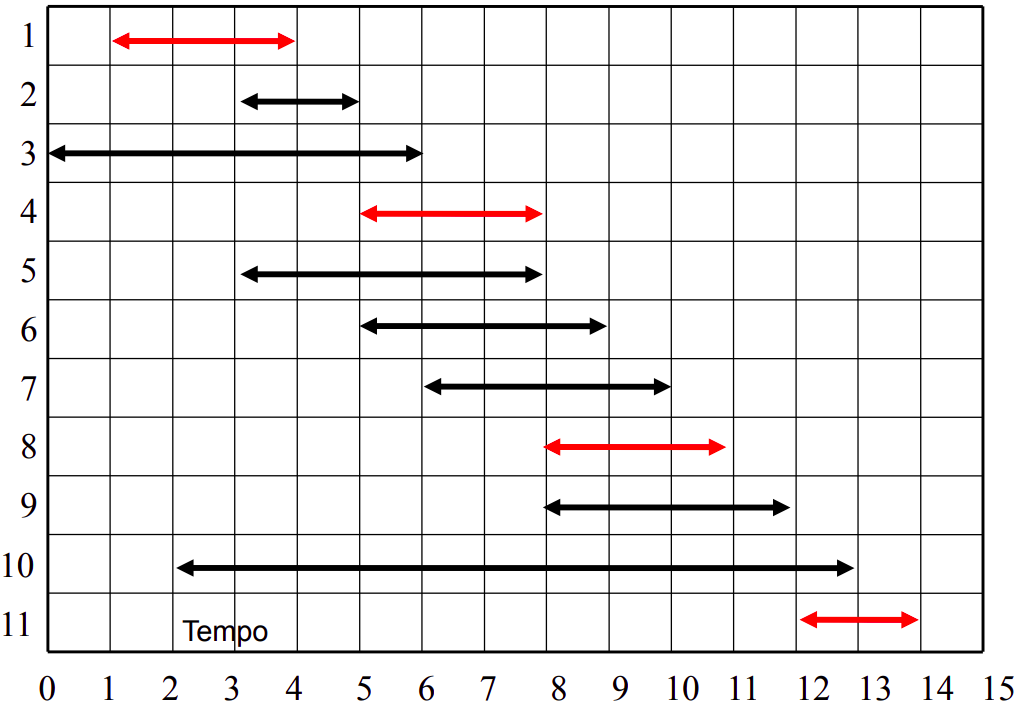
\includegraphics[width=0.45\textwidth]{intervalli-ordinati-greedy1.png}
    \caption{Possibile soluzione}
\end{figure}

\subsection{Approccio basato su programmazione dinamica}
Iniziamo ricercando una \emph{sottostruttura ottima}. Assumiamo che gli intervalli
siano ordinati per tempo di fine:
\[b_1\leq\dots\leq b_n\]
Definiamo il sotto-problema $S[i\dots j]$ come l'insieme di intervalli che
iniziano dopo la fine di $i$ e finiscono prima dell'inizio di $j$:
\[S[i\dots j]=\{k\;|\;b_i\leq a_k<b_k\leq a_j\}\]
Aggiungiamo due intervalli fittizi:
\begin{itemize}
    \item \emph{Intervallo $0$}: $b_0=-\infty$;
    \item \emph{Intervallo $n+1$}: $a_{n+1}=+\infty$;
\end{itemize}
Il problema generale corrisponde quindi al problema $S[0\dots n+1]$.

\begin{definition}[Sottostruttura ottima]
    Supponiamo che $A[i\dots j]$ sia una soluzione ottimale di $S[i\dots j]$
    e sia $k$ un intervallo che appartiene ad $A[i\dots j]$. Allora:
    \begin{itemize}
        \item Il problema $S[i\dots j]$ può essere suddiviso in due intervalli:
        \begin{enumerate}
            \item $S[i\dots k]$ contenente gli intervalli di $S[i\dots j]$ che
            finiscono prima di $k$;
            \item $S[k\dots j]$ contenente gli intervalli di $S[i\dots j]$ che
            iniziano dopo $k$;
        \end{enumerate}
        \item $A[i\dots j]$ contiene le soluzioni ottimali di $S[i\dots k]$ e
        $S[k\dots j]$:
        \begin{enumerate}
            \item $A[i\dots j]\cap S[i\dots k]$ è la soluzione ottimale di $A[i\dots k]$;
            \item $A[i\dots j]\cap S[k\dots j]$ è la soluzione ottimale di $A[k\dots j]$;
        \end{enumerate}
    \end{itemize}
\end{definition}

\noindent
Quanto detto ci permette di definire $A[i\dots j]$ come:
\[A[i\dots j]=A[i\dots k]\cup\{k\}\cup A[k\dots j]\]
Per determinare $k$ proviamo tutte le possibilità. A questo punto, sia $DP[i][j]$
la dimensione del più grande sottoinsieme $A[i\dots j]\subseteq S[i\dots j]$ di
intervalli indipendenti. Possiamo definire $DP[i][j]$ con la seguente funzione
ricorsiva:
\[DP[i][j]=\begin{cases}
    0 & S[i\dots j]=\emptyset\\
    \max_{k\in S[i\dots j]}\{DP[i][k]+DP[k][j]+1\} & \text{altrimenti}
\end{cases}\]
Questa definizione ci permette di realizzare un algoritmo basato su
\emph{programmazione dinamica}, o su \emph{memoization}, con \emph{complessità}
pari a $O(n^3)$. Questo perché bisogna risolvere tutti i problemi con $i<j$ e,
nel caso peggiore, paghiamo $O(n)$ per ogni sotto-problema.

\bigskip\noindent
Possiamo fare meglio di così?

Potremmo semplicemente usare la soluzione al problema con pesi generici, che
ha \emph{complessità} $O(n\log n)$, ponendo a $1$ tutti i pesi. Tuttavia,
potremmo anche chiederci se sia davvero necessario analizzare tutti i
possibili valori di $k$. Definiamo il seguente teorema:

\begin{definition}[Scelta ingorda]
    Siano $S[i\dots j]$ un sotto-problema non vuoto e $m$ l'intervallo di $S[i\dots
    j]$ con il minor tempo di fine. Allora, valgono i due seguenti punti:
    \begin{enumerate}
        \item Il sotto-problema $S[i\dots m]$ è vuoto;
        \item $m$ è compreso in una qualche soluzione ottima di $S[i\dots j]$,
        ovvero $m\in A[i\dots j]$;
    \end{enumerate}
\end{definition}
\begin{proof}[Dimostrazione]
    Dimostriamo separatamente i due punti.

    \paragraph{Punto 1 - \bm{$S[i$}\dots\bm{$ j]=\emptyset$}}
    Per la definizione di intervallo sappiamo che $a_m<b_m$. Inoltre, poiché $m$
    è l'intervallo con il minor tempo di fine, $\forall k\in S[i\dots j]$ $b_m
    \leq b_k$ e quindi, ne consegue che $\forall k\in S[i\dots j]$ $a_m<b_k$.
    Se nessun intervallo in $S[i\dots j]$ termina prima di $a_m$, allora $S[i
    \dots m]=\emptyset$.

    \paragraph*{Punto 2 - \bm{$m\in A[i$}\dots\bm{$i]$}}
    Siano $A'[i\dots j]$ una soluzione ottima di $S[i\dots j]$ e $m'$ l'intervallo
    con minor tempo di fine in $A'[i\dots j]$. Sia ora $A[i\dots j]=A'[i\dots j]
    -\{m'\}\cup\{m\}$ una nuova soluzione ottima ottenuta togliendo $m'$ e
    aggiungendo $m$ ad $A'[i\dots j]$. $A[i\dots j]$ è una soluzione ottima che
    contiene $m$ in quanto ha la stessa cardinalità di $A'[i\dots j]$ e gli
    intervalli sono indipendenti.
\end{proof}

\noindent
Questa dimostrazione ci permette di selezionare sempre gli intervalli con tempo
di fine minore e ignorare tutti quelli che si intersecano con esso, riducendo
il problema alla ricerca dell'\emph{insieme indipendente massimale} in $S[m\dots
j]$.

\begin{figure}[h!]
    \centering
    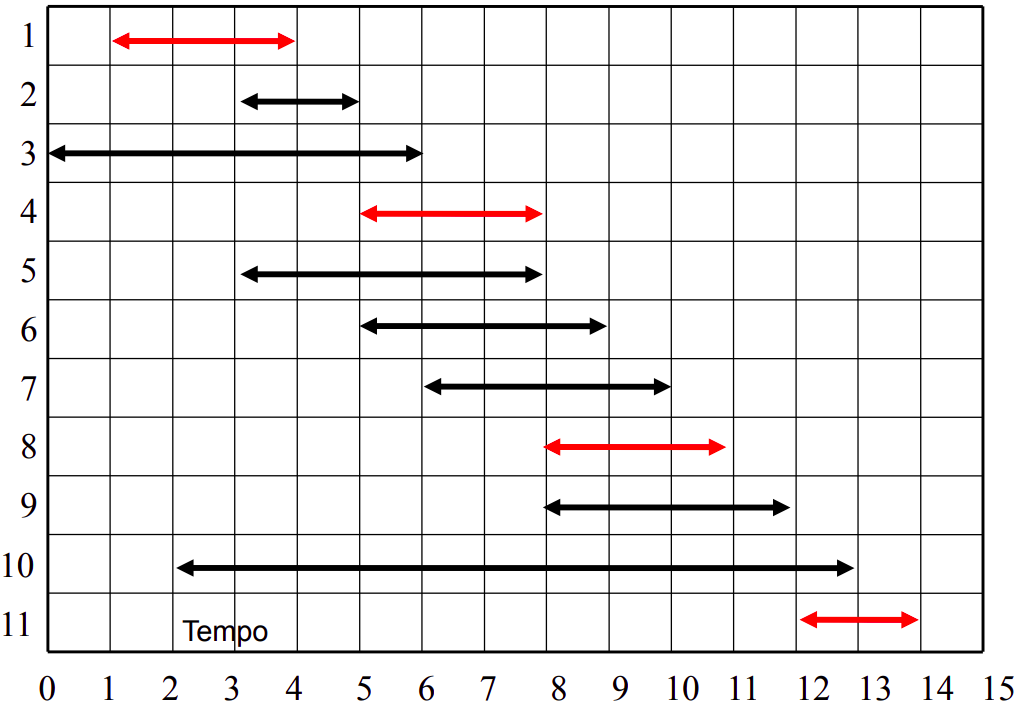
\includegraphics[width=0.45\textwidth]{intervalli-ordinati-greedy1.png}
    \caption{Soluzione con \emph{scelte ingorde}}
\end{figure}

\begin{minicode}{Soluzione basata su programmazione greedy}
\ind\bc{SET} indipendentSet(\bc{int}[] a, \bc{int}[] b)\\
    \{ Ordina i vettori $a$ e $b$ in modo che $b_1\leq\dots\leq b_n$ \}\\
    \bc{SET} S = Set()\\
    S.insert(1)\\
    \bc{int} last = 1\\
    \indf for (i = 2 to n) do\\
        \indff if (a[i] $\geq$ b[last]) then\\
            S.insert(i)\\
            last = i\\
    \indf return S
\end{minicode}

\paragraph{Complessità}
Questa soluzione abbassa la \emph{complessità} a $O(n)$ se i vettori di input
sono già ordinati, $O(n\log n)$ altrimenti.

\begin{eg}[Esempio d'esecuzione]
    Il comportamento del nuovo algoritmo con gli stessi intervalli degli esempi
    precedenti è il seguente:

    \begin{figure}[h!]
        \centering
        \subfloat{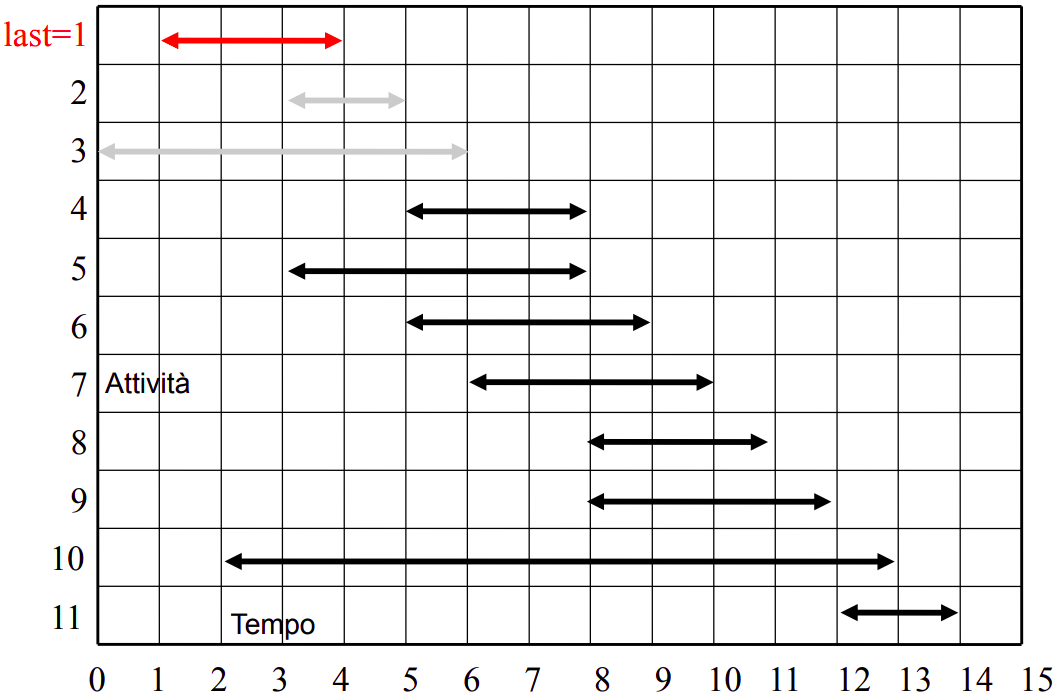
\includegraphics[width=0.48\textwidth]
        {intervalli-ordinati-greedy-s1.png}}
        \hfill
        \subfloat{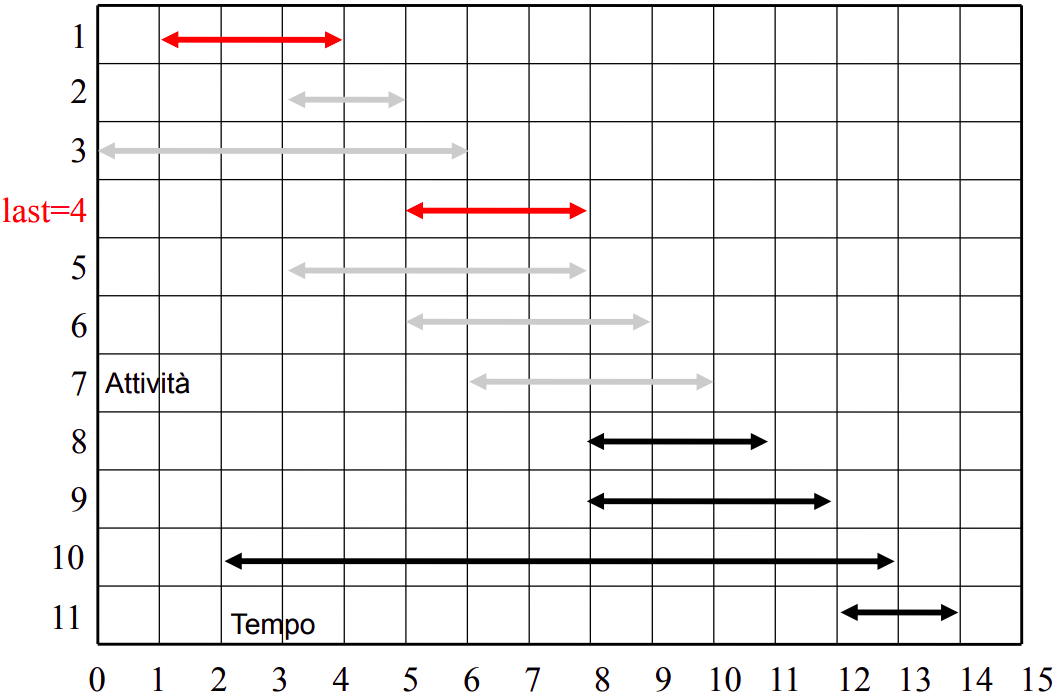
\includegraphics[width=0.48\textwidth]
        {intervalli-ordinati-greedy-s2.png}}\\
        \subfloat{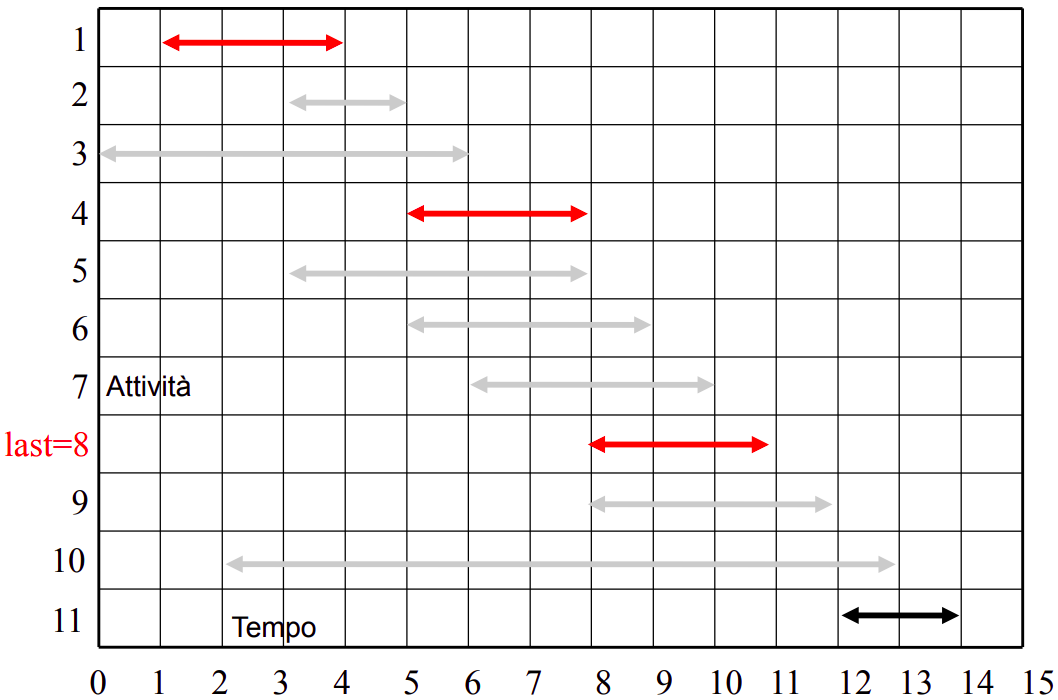
\includegraphics[width=0.48\textwidth]
        {intervalli-ordinati-greedy-s3.png}}
        \hfill
        \subfloat{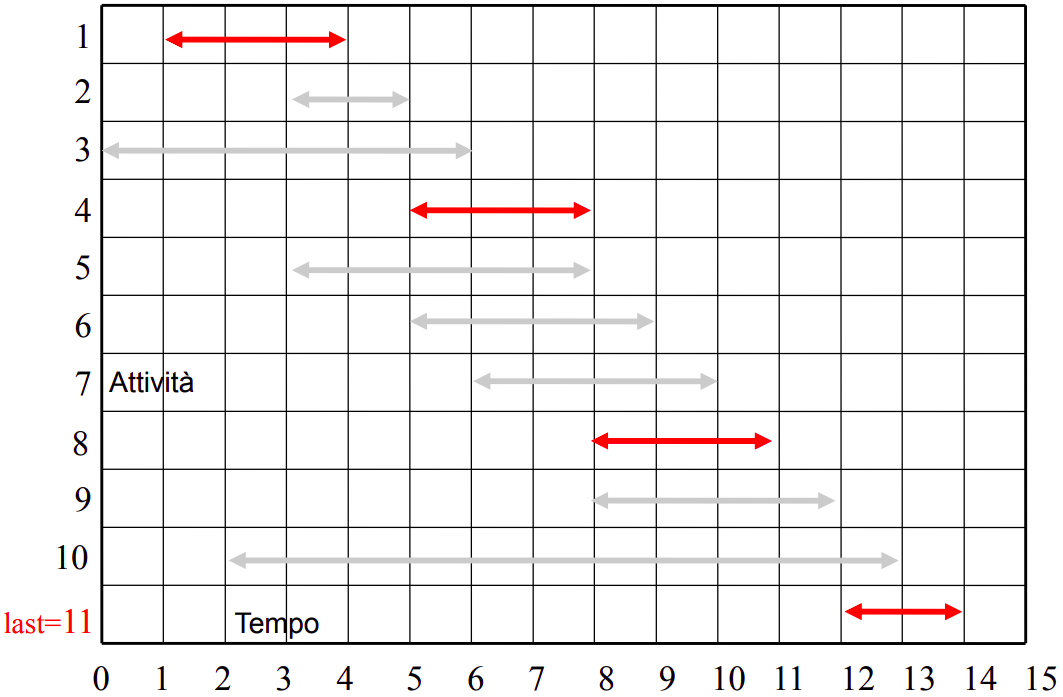
\includegraphics[width=0.48\textwidth]
        {intervalli-ordinati-greedy-s4.png}}
    \end{figure}
\end{eg}

\section{Problema dello scheduling}
\begin{problem}[Scheduling dei processi]
    Dati un processore e $n$ processi da eseguire su di esso. Se ogni processo $i$
    è caratterizzato da un tempo d'esecuzione $t[i]$ noto a priori, trovare una
    sequenza d'esecuzione che minimizzi il tempo di completamento medio.
\end{problem}
\begin{definition}[Tempo di completamento]
    Dato un vettore $A[1\dots n]$ contenente una permutazione di $\{1\dots n\}$,
    il tempo di completamento dell'$h$-esimo processo nella permutazione è
    calcolato come:
    \[T_A(h)=\sum_{i=1}^h t[A[i]]\]
\end{definition}

\newpage
\begin{eg}[Possibili permutazioni]
    Consideriamo i seguenti processi con relativo tempo d'esecuzione:
    
    \begin{table}[h!]
        \centering
        \renewcommand{\arraystretch}{1.2}
        \begin{tabular}{|c|c|c|c|c|}
            \hline
            \textbf{Processo} & $1$ & $2$ & $3$ & $4$\\
            \hline
            \bm{$t[i]$} & 4 & 1 & 6 & 3\\
            \hline
        \end{tabular}    
    \end{table}

    \noindent
    Se eseguissimo i processi nell'ordine $A[1,2,3,4]$ la situazione sarebbe
    la seguente:

    \begin{figure}[h!]
        \centering
        \begin{graph}
            \tikzset{
                cell/.style={rectangle, draw, minimum size=10mm, anchor=west},
            }
            \node[cell] (1) [minimum width=40mm, label={[xshift=-12mm]225:{$0$}}] {$4$};
            \node[cell] (2) [minimum width=10mm, right of=1, xshift=5mm,
            label={[xshift=3mm]225:{$4$}}, label={[xshift=-3mm]-45:{$5$}}] {$1$};
            \node[cell] (3) [minimum width=60mm, right of=2, xshift=15mm,
            label={[xshift=21.5mm]-45:{$11$}}] {$6$};
            \node[cell] (4) [minimum width=30mm, right of=3, xshift=25mm,
            label={[xshift=6mm]-45:{$14$}}] {$3$};
        \end{graph}
    \end{figure}

    \noindent
    Il tempo di completamento medio sarebbe:
    \[\frac{\sum_{i=1}^4 T_A(i)}{4}=\frac{4+5+11+14}{4}=\frac{34}{4}=8.5\]
    Se invece ordinassimo i processi per tempo d'esecuzione crescente, ponendo
    $A=[2,4,1,3]$, la situazione diventerebbe:
    
    \begin{figure}[h!]
        \centering
        \begin{graph}
            \tikzset{
                cell/.style={rectangle, draw, minimum size=10mm, anchor=west},
            }
            \node[cell] (2) [minimum width=10mm, label={[xshift=3mm]225:{$0$}},
            label={[xshift=-2.5mm]-45:{$1$}}] {$1$};
            \node[cell] (4) [minimum width=30mm, right of=2,
            label={[xshift=7mm]-45:{$5$}}] {$3$};
            \node[cell] (1) [minimum width=40mm, right of=4, xshift=15mm,
            label={[xshift=12mm]-45:{$8$}}] {$4$};
            \node[cell] (3) [minimum width=60mm, right of=1, xshift=30mm,
            label={[xshift=21.5mm]-45:{$14$}}] {$6$};
        \end{graph}
    \end{figure}

    \noindent
    Il tempo di completamento medio adesso è:
    \[\frac{\sum_{i=1}^4 T_A(i)}{4}=\frac{1+5+8+14}{4}=\frac{27}{4}=6.75\]
\end{eg}
\begin{note}
    Dall'esempio intuiamo che la scelta ottima potrebbe essere quella di
    prendere sempre il processo con minor \emph{tempo d'esecuzione}.
\end{note}

\begin{definition}[Scelta ingorda]
    Esiste una soluzione ottima $A$ in cui il processo con minor tempo
    d'esecuzione si trova in prima posizione.
\end{definition}

\begin{definition}[Sottostruttura ottima]
    Sia $A$ una soluzione ottima di un problema con $n$ processi, in cui il
    processo con minor tempo d'esecuzione $m$ si trova in prima posizione. La
    permutazione dei seguenti $n-1$ processi è una soluzione al sotto-problema
    in cui $m$ non viene considerato.
\end{definition}
\begin{proof}[Dimostrazione]
    Consideriamo una \emph{permutazione ottima} $A$:
    \[A=[A[1],\dots A[m],\dots,A[n]]\]
    Siano $m$ l'indice del processo con minor \emph{tempo d'esecuzione} e
    $A'$ una permutazione in cui i processi in posizione $1$ e $m$ vengono
    scambiati, ovvero:
    \[A=[A[m],\dots,A[1],\dots,A[n]]\]
    Il \emph{tempo di completamento medio} di $A'$ è minore o uguale a quello di
    $A$. Questo è vero perché i processi nelle posizioni $1,\dots,m-1$ in $A'$
    hanno un \emph{tempo di completamento} minore o uguale a quello dei processi
    in posizione $1,\dots,m-1$ in $A$. D'altra parte, i processi nelle posizioni
    $m,\dots,n$ hanno lo stesso \emph{tempo di completamento} sia in $A$ che in
    $A'$.

    Ora, poiché avevamo ipotizzato che $A$ fosse una \emph{permutazione ottima},
    il suo \emph{tempo di completamento medio} non può essere superiore a quello
    di $A'$, quindi anche $A'$ è una \emph{permutazione ottima}.
\end{proof}

\section{Problema dello zaino frazionario}
Consideriamo una variante del \emph{\hyperref[prob:7]{problema dello zaino}}
in cui è possibile prendere frazioni di oggetti.

\begin{eg}[Possibili ordinamenti degli oggetti]
    Consideriamo uno zaino con capacità 70 e di avere i tre oggetti seguenti:

    \begin{table}[h!]
        \centering
        \renewcommand{\arraystretch}{1.2}
        \begin{tabular}{|c|c|c|}
            \hline
            \bm{$i$} & \bm{$p_i$} & \bm{$w_i$}\\
            \hline
            1 & 60 & 10\\
            \hline
            2 & 200 & 40\\
            \hline
            3 & 120 & 30\\
            \hline
        \end{tabular}
    \end{table}

    \noindent
    Per prendere gli oggetti possiamo provare a ordinarli in qualche modo
    così poter operare una scelta ponderata sul tipo di ordinamento applicato.

    \paragraph{Ordinamento per profitto decrescente}
    In questo modo andiamo a scegliere gli oggetti $2$ e $3$ ottenendo un
    guadagno totale di $320$.

    \paragraph{Ordinamento per peso crescente}
    Questo approccio ci porta a scegliere la totalità degli oggetti $1$
    e $3$, per un peso di $40$. Per usare la rimanente capacità prendiamo i
    $\frac{3}{4}$ dell'oggetto $2$. Il profitto che otteniamo sale quindi a
    $330$.

    \paragraph{Ordinamento per profitto specifico decrescente}
    Definiamo il profitto specifico come il rapporto $\frac{p_i}{w_i}$. Per gli
    oggetti $1$, $2$, $3$ il profitto specifico vale $6$, $5$ e $4$ rispettivamente.
    Di conseguenza, prendiamo la totalità degli oggetti $1$ e $2$ e i $\frac{2}{3}$
    dell'ultimo oggetto. Questa scelta ci assicura un guadagno di $340$.
\end{eg}
\begin{minicode}{Implementazione della soluzione}
\ind\bc{float}[] zaino(\bc{float}[] p, \bc{float}[] w, \bc{float} C, \bc{int} n)\\
    \bc{float}[] x = new \bc{float}[1\dots n]\hfill\com{Vettore delle quantità raccolte}
    \{ Ordina $p$ e $w$ in modo che $p[1]/w[1]\geq\dots\geq p[n]/w[n]$ \}\\
    \indf for (i = 1 to n) do\\
        x[i] = min(C / w[i], 1)\\
        C = C - x[i] $\cdot$ w[i]\\
    \indf return x
\end{minicode}

\paragraph{Complessità}
La \emph{complessità} è $O(n)$ se i vettori di input sono già ordinati, $O(n\log
n)$ altrimenti.

\bigskip\noindent
Abbiamo definito l'algoritmo, ma in realtà non abbiamo ancora dimostrato che
quel tipo di scelta sia corretta.

\begin{proof}[Dimostrazione]
    Assumiamo che gli oggetti siano ordinati per \emph{profitto specifico
    decrescente}. Sia $x$ una soluzione ottima e supponiamo che $x[1]<\min\left(
    \frac{C}{w[i]}, 1\right)<1$. Allora, possiamo costruire una nuova soluzione
    in cui $x'[1]=\min\left(\frac{C}{w[i]}, 1\right)$ e la porzione di uno o
    più oggetti è ridotta di conseguenza. La soluzione $x'$ è sicuramente di
    profitto uguale o maggiore rispetto ad $x$ perché il \emph{profitto
    specifico} del primo oggetto è massimo.
\end{proof}

\section{Problema della compressione}
Quello della compressione dei dati è una problema classico dell'informatica.
Una delle possibili tecniche per la compressione dei caratteri\footnote{Per
le immagini esistono tecniche migliori} è tramite una \emph{funzione di codifica}
del tipo $f:f(c)=x$ in cui $c$ è un carattere preso da un alfabeto $\Sigma$ e
$x$ è la sua rappresentazione binaria.

\begin{note}
    $\Sigma$ può essere definito come l'insieme dei caratteri usati all'interno
    di un file da comprimere.
\end{note}

\begin{eg}[Possibili compressioni]
    Supponiamo di avere un file di $n$ caratteri, che $\Sigma=\{a,b,c,d,e,f\}$ e
    di conoscere la frequenza di ogni carattere.

    \begin{table}[h!]
        \centering
        \renewcommand{\arraystretch}{1.2}
        \begin{adjustbox}{max width=0.98\textwidth}
        \begin{tabular}{|c|c|c|c|c|c|c|c|}
            \hline
            \textbf{Caratteri} & \bc{\texttt{a}} & \bc{\texttt{b}} &
            \bc{\texttt{c}} & \bc{\texttt{d}} & \bc{\texttt{e}} &
            \bc{\texttt{f}} & \textbf{Dimensione}\\
            \hline
            \textbf{Frequenza} & 45\% & 13\% & 12\% & 16\% & 9\% & 5\% & \\
            \hline
            \textbf{ASCII} & \texttt{01100001} & \texttt{01100010} &
            \texttt{01100011} & \texttt{01100100} & \texttt{01100101} &
            \texttt{01100110} & 8n\\
            \hline
            \textbf{Codifica 1} & \texttt{000} & \texttt{001} & \texttt{010} &
            \texttt{011} & \texttt{100} & \texttt{101} & 3n\\
            \hline
            \textbf{Codifica 2} & \texttt{0} & \texttt{101} & \texttt{100} &
            \texttt{111} & \texttt{1101} & \texttt{1100} & 2.24n\\
            \hline
        \end{tabular}
    \end{adjustbox}
    \end{table}
    
    \noindent
    Nella codifica 1 abbiamo codificato i caratteri usando il numero minimo
    di bit necessari per rappresentare 6 valori. Per quanto riguarda la
    codifica 2 invece, abbiamo calcolato la dimensione totale come:
    \[\left(0.45\cdot1+0.13\cdot3+0.12\cdot3+0.16\cdot3+0.09\cdot4+0.05\cdot
    4\right)n=2.24n\]
\end{eg}

\begin{definition}[Codice a prefisso]
    In un codice a prefisso, nessun codice è prefisso di un altro.
\end{definition}\noindent
La caratteristica dei \emph{codici a prefisso} è necessaria per consentire la
decodifica.

\begin{eg}[Codici a prefisso e non]
    Consideriamo un codice del tipo:
    \[a\to0,\,b\to 10,\,c\to11\]
    La codifica per la stringa \texttt{babaca} è:
    \[10\ 0\ 10\ 0\ 11\ 0\]
    che può essere decodificata senza ambiguità percorrendola da sinistra, in
    quanto, appena viene riscontrata la corrispondenza con un carattere, si
    può sostituire quel carattere alla sua codifica sapendo che i bit successivi
    costituiranno la rappresentazione di un altro carattere.

    \bigskip\noindent
    Nel caso di un codice di questo tipo invece:
    \[a\to0,\, b\to1,\,c\to 11\]
    dovendo decodificare la sequenza di bit:
    \[111111\]
    si crea un'ambiguità, in quanto un singolo bit $1$ rappresenta la $b$, mentre
    due bit rappresentano la $c$.
\end{eg}

\subsection{Algoritmo di Huffman}
L'\emph{Algoritmo di Huffman} utilizza rappresentazioni ad albero per definire
il codice di codifica a partire dal testo e per ritornare al testo originale a
partire dalla codifica. In particolare, viene usato un \emph{albero binario}
in cui al ramo sinistro di ciascun \emph{nodo} è associato il bit 0, viceversa
al ramo destro è sempre associato il bit 1. I caratteri si trovano nelle
\emph{foglie} e il \emph{cammino} che si percorre per andare dalla \emph{radice}
a ciascuna \emph{foglia} corrisponde alla codifica del carattere associato.

\begin{figure}[h!]
    \centering
    \hspace{5mm}
    \begin{minipage}{0.48\textwidth}
    \begin{graph}
        \node[main] (0) {};
        \node[main] (1) [below left of=0, xshift=-20, yshift=-20] {};
        \node[main] (2) [below right of=0, xshift=20, yshift=-20] {};
        \node[main] (3) [below left of=1, xshift=0, yshift=-20] {$a$};
        \node[main] (4) [below right of=1, xshift=0, yshift=-20] {};
        \node[main] (5) [below left of=2, xshift=0, yshift=-20] {$d$};
        \node[main] (6) [below right of=2, xshift=0, yshift=-20] {$e$};
        \node[main] (9) [below left of=4, xshift=20, yshift=-20] {$b$};
        \node[main] (10) [below right of=4, xshift=-20, yshift=-20] {$c$};
      
        \path[-]  (0) edge node [above left] {$0$} (1)
                  (0) edge node [above right] {$1$} (2)
                  (1) edge node [above left] {$0$} (3)
                  (1) edge node [above right] {$1$} (4)
                  (2) edge node [above left] {$0$} (5)
                  (2) edge node [above right] {$1$} (6)
                  (4) edge node [left] {$0$} (9)
                  (4) edge node [right] {$1$} (10);
    \end{graph}
    \end{minipage}
    \hfill
    \begin{minipage}{0.45\textwidth}
    \renewcommand{\arraystretch}{1.2}
    \begin{tabular}{|c|c|c|c|c|c|}
        \hline
        \textbf{Carattere} & $a$ & $b$ & $c$ & $d$ & $e$\\
        \hline
        \textbf{Codifica} & $00$ & $010$ & $011$ & $10$ & $11$\\
        \hline
    \end{tabular}
    \end{minipage}
    \caption{Esempio di \emph{albero binario di decodifica}}
\end{figure}

\noindent
Questa rappresentazione ci permette di legare il numero di bit necessari per
codificare un carattere alla \emph{profondità} della \emph{foglia} ad esso
associata all'interno dell'\emph{albero}.

\paragraph{Numero di bit necessari a codificare un file}
In particolare, se $\Sigma$ è l'alfabeto di un file $F$ e $T$ è un albero
che rappresenta la codifica, per ogni carattere $c\in\Sigma$, $d_T(c)$
rappresenta la \emph{profondità} della \emph{foglia} associata a $c$ in $T$.
Dunque, la codifica di $c$ richiede $d_T(c)$ bit e, se $f[c]$ è il numero di
occorrenze di $c$ in $F$, la dimensione della codifica per l'intero file è:
\[C(F,T)=\sum_{c\in\Sigma}f[c]\cdot d_T(c)\]

\paragraph{Principi dell'Algoritmo di Huffman}
L'idea alla base dell'\emph{Algoritmo di Huffman} è quella di minimizzare la
lunghezza delle codifiche per i caratteri che compaiono più frequentemente e,
al contrario, assegnare ai caratteri con la frequenza minore i codici
corrispondenti ai percorsi più lunghi all'interno dell'\emph{albero}.

\begin{note}
    Ogni codifica è associata a un solo file.
\end{note}

\noindent
Ad ogni \emph{nodo} dell'\emph{albero} viene associato un carattere con la
relativa frequenza. La costruzione dell'\emph{albero} procede per aggregazione
delle coppie di \emph{nodi} con frequenza minima. Ad ogni iterazione, i due
\emph{nodi} $x$, $y$ con frequenza $f_x$ e $f_y$ minori vengono resi
\emph{figli} di un nuovo \emph{nodo} fittizio con frequenza $f_x+f_y$. Questo
\emph{nodo} viene quindi aggiunto all'insieme iniziale di caratteri. L'algoritmo
continua in questo modo fino a quando non rimane un solo \emph{nodo} e termina
dopo aver etichettato gli \emph{archi}.

\begin{figure}[h!]
    \centering
    \subfloat[\emph{Nodi} iniziali]{\resizebox{0.48\textwidth}{!}{
    \begin{graph}
        \node[main] (a) [label=above:{$45$}, yshift=-8mm] {$a$};
        \node[main] (b) [label=above:{$13$}, right of=a] {$b$};
        \node[main] (c) [label=above:{$12$}, right of=b] {$c$};
        \node[main] (d) [label=above:{$16$}, right of=c] {$d$};
        \node[main] (e) [label=above:{$9$}, right of=d] {$e$};
        \node[main] (f) [label=above:{$5$}, right of=e] {$f$};

        \node[] (1) [below of=a] {};
    \end{graph}
    }}
    \hfill
    \subfloat[Prima aggregazione]{\resizebox{0.46\textwidth}{!}{
    \begin{graph}
        \node[main] (a) [label=above:{$45$}] {$a$};
        \node[main] (b) [label=above:{$13$}, right of=a] {$b$};
        \node[main] (c) [label=above:{$12$}, right of=b] {$c$};
        \node[main] (d) [label=above:{$16$}, right of=c] {$d$};
        \node[main] (ef) [label=above:{$14$}, right of=d] {$-$};
        \node[main] (e) [label=below:{$9$}, below right of=ef, yshift=-5mm] {$e$};
        \node[main] (f) [label=below:{$5$}, below left of=ef, yshift=-5mm] {$f$};

        \path[-]    (ef) edge (e)
                    (ef) edge (f);
    \end{graph}
    }}\\
    \subfloat[\emph{Albero} al termine della costruzione]{
    \begin{graph}
        \node[main] (0) [label=above:{$100$}] {$-$};
        \node[main] (a) [label=below:{$45$}, below left of=0, yshift=-5mm,
            xshift=-15mm] {$a$};
        \node[main] (1) [label=above:{$55$}, below right of=0, yshift=-5mm,
            xshift=15mm] {$-$};
        \node[main] (2) [label=above:{$25$}, below left of=1, yshift=-5mm,
            xshift=-10mm] {$-$};
        \node[main] (3) [label=above:{$30$}, below right of=1, yshift=-5mm,
            xshift=10mm] {$-$};
        \node[main] (b) [label=below:{$13$}, below right of=2, yshift=-5mm] {$b$};
        \node[main] (c) [label=below:{$12$}, below left of=2, yshift=-5mm] {$c$};
        \node[main] (d) [label=below:{$16$}, below right of=3, yshift=-5mm] {$d$};
        \node[main] (4) [label=above:{$14$}, below left of=3, yshift=-5mm] {$-$};
        \node[main] (e) [label=below:{$9$}, below right of=4, yshift=-5mm] {$e$};
        \node[main] (f) [label=below:{$5$}, below left of=4, yshift=-5mm] {$f$};

        \path[-]    (0) edge node [above left] {$0$} (a)
                    (0) edge node [above right] {$1$} (1)
                    (1) edge node [above left] {$0$} (2)
                    (1) edge node [above right] {$1$} (3)
                    (2) edge node [above left] {$0$} (c)
                    (2) edge node [above right] {$1$} (b)
                    (3) edge node [above left] {$0$} (4)
                    (3) edge node [above right] {$1$} (d)
                    (4) edge node [above left] {$0$} (f)
                    (4) edge node [above right] {$1$} (e);
    \end{graph}
    }
\end{figure}
\noindent
La codifica ottenuta è quindi:
\begin{table}[h!]
    \centering
    \renewcommand{\arraystretch}{1.2}
    \begin{tabular}{|c|c|c|c|c|c|c|}
        \hline
        \textbf{Carattere} & $a$ & $b$ & $c$ & $d$ & $e$ & $f$\\
        \hline
        \textbf{Codifica} & $0$ & $101$ & $100$ & $111$ & $1101$ &  $1100$\\
        \hline
    \end{tabular}
\end{table}

\newpage
\begin{minicode}{Algoritmo di Huffman}
\ind\bc{TREE} huffman(\bc{int}[] c, \bc{int}[] f, \bc{int} n)\\
    \bc{PRIORITYQUEUE} Q = MinPriorityQueue()\\
    \indf for (i = 1 to n) do\\
        \com{Inserisco nella \emph{coda} il \emph{nodo} $c[i]$ con \emph{priorità} $f[i]$}
        Q.insert(f[i], Tree(f[i], c[i]))\\
    \indf for (i = 1 to n - 1) do\\
        z$_1$ = Q.deleteMin()\\
        z$_2$ = Q.deleteMin()\\
        z = Tree(z$_1$.f, z$_2$.f, nil)\hfill\com{Crea il \emph{nodo} fittizio}
        z.insertLeft(z$_1$)\\
        z.insertRight(z$_2$)\\
        Q.insert(z.f, z)\hfill\com{Rimette il \emph{nodo} fittizio nella \emph{coda}}
    \indf return Q.deleteMin()
\end{minicode}
\begin{note}
    In questo frammento ipotizziamo che ad ogni \emph{nodo} sia possibile
    associare una frequenza oltre che un valore. La firma della funzione
    \texttt{Tree} è quindi \texttt{Tree(\bc{int} frequence, \bc{ITEM} value)}.
    Oltre a ciò, ipotizziamo che sia possibile accedere alla frequenza di un
    \emph{nodo} mediante un attributo \texttt{f}.
\end{note}

\paragraph{Complessità}
La costruzione dell'\emph{albero} attraverso l'uso di \emph{code a priorità}
costa $O(n\log n)$, quindi la \emph{complessità} finale è $T(n)=O(n\log n)$.

\bigskip\noindent
Come al solito, dobbiamo dimostrare la correttezza dell'approccio scelto. In
particolare, dobbiamo dimostrare che costruire un \emph{albero} scegliendo
sempre i due caratteri con frequenza minore conduce sempre ad una soluzione
ottimale. Inoltre, dobbiamo dimostrare che questa soluzione gode di una
\emph{sottostruttura ottima}, per la quale, dato un problema sull'alfabeto
$\Sigma$, è possibile costruire un sotto-problema con un alfabeto più piccolo
aggregando i due caratteri con frequenza minore. Quanto detto è riassumibile
nel seguente teorema:
\begin{definition}[Teorema per la correttezza dell'Algoritmo di Huffman]
    Dato un alfabeto $\Sigma$ e un vettore delle frequenze $f$, se $x$ e $y$
    sono i due caratteri con frequenza minore, esiste un codice ottimo per
    $\Sigma$ in cui $x$ e $y$ hanno la stessa profondità massima e i loro codici
    differiscono solo per l'ultimo bit.
\end{definition}
\begin{proof}[Dimostrazione]
    Supponiamo che esista una codice ottimo $T$ in cui i due caratteri $a$ e $b$
    con \emph{profondità massima} siano diversi da $x$ e $y$. Possiamo assumere
    senza perdere di generalità che:
    \[f[x]\leq f[y]\wedge f[a]\leq f[b]\]
    Poiché le frequenze di $x$ e $y$ sono minime, vale:
    \[f[x]\leq f[a]\wedge f[y]\leq f[b]\]
    Se scambiamo $x$ ed $a$ otteniamo una soluzione $T'$ e se poi scambiamo
    anche $y$ e $b$ otteniamo una terza soluzione $T''$. A questo punto,
    dimostriamo che $C(f,T'')\leq C(f,T')\leq C(f,T)$:
    \[C(f,T)-C(f,T')\begin{array}[t]{cl}
        = & \sum_{c\in\Sigma} f[c]d_T(c)-\sum_{c\in\Sigma}f[c]d_{T'}(c)\\
        = & \left(f[x]d_T(x)-f[a]d_{T}(a)\right)-\left(f[x]d_{T'}(x)-
        f[a]d_{T'}(a)\right)\\
        = & \left(f[x]d_T(x)-f[a]d_{T}(a)\right)-\left(f[x]d_{T}(a)-
        f[a]d_{T}(x)\right)\\
        = & \left(f[a]-f[x]\right)\cdot\left(d_T(a)-d_T(x)\right)\\
        \leq & 0
    \end{array}\]
    Allo stesso modo possiamo dimostrare che $C(f,T')-C(f,T'')\geq 0$, ma
    poiché $T$ è ottimo deve valere anche $C(f,T)\leq C(f,T'')$ e quindi anche
    $T''$ è una soluzione ottima.
\end{proof}

\section{Ricerca degli alberi di copertura di peso minimo}
\begin{problem}[Ricerca dell'albero di copertura di peso minimo]
    Dati un grafo $G=(V,E)$ non orientato e una funzione di peso $w:V\times
    V\to\mathbb{R}$, determinare il modo di interconnettere tutti i suoi
    nodi che minimizzi il peso totale dei suoi archi.
\end{problem}
\begin{note}
    Questo tipo di \emph{alberi} prende anche il nome di \emph{minimum spanning
    tree} e \emph{alberi di connessione di peso minimo}.
\end{note}

\noindent
La funzione di peso $w$ può essere meglio definita dicendo che se $(u,v)\in E$,
allora $w(u,v)$ sarà pari al peso dell'\emph{arco} da $u$ a $v$. Altrimenti,
assume valore $+\infty$. Inoltre, poiché il \emph{grafo} è \emph{non orientato},
$w(u,v)=w(v,u)$. Poiché ricerchiamo l'\emph{albero di peso minimo}, il peso totale
della soluzione $T$, definito come:
\[w(T)=\sum_{(u,v)\in E_T}w(u,v)\]
deve essere minimo rispetto al peso di tutti gli altri \emph{alberi di copertura}
definibili su quel \emph{grafo}.

\begin{note}
    L'\emph{albero di copertura di peso minimo} non corrisponde necessariamente
    con l'\emph{albero di copertura} associato ai \emph{cammini minimi} da un
    \emph{nodo} a tutti gli altri.

    \begin{figure}[h!]
        \centering
        \subfloat[\emph{Albero di copertura dei cammini minimi}]{
        \begin{graph}
            \node[main, line width=1.2pt] (a) [label={$d[A]=0$}] {$A$};
            \node[main] (b) [right of=a, label={$d[B]=3$}, xshift=10mm] {$B$};
            \node[main] (c) [below of=b, label=below:{$d[C]=4$}, yshift=-10mm] {$C$};
            \node[main] (d) [left of=c, label=below:{$d[D]=3$}, xshift=-10mm] {$D$};
    
            \path[->]
                        (a) edge[line width=1.2pt] node[above] {$3$} (b)
                        (b) edge[line width=1.2pt] node[right] {$1$} (c)
                        (a) edge[line width=1.2pt] node[left] {$3$} (d);
            \path[-]    (d) edge node[below] {$2$} (c);
        \end{graph}
        }
        \hspace{3cm}
        \subfloat[\emph{Albero di copertura di peso minimo}]{
        \begin{graph}
            \node[main, line width=1.2pt] (a) [label={$d[A]=0$}] {$A$};
            \node[main] (b) [right of=a, label={$d[B]=3$}, xshift=10mm] {$B$};
            \node[main] (c) [below of=b, label=below:{$d[C]=4$}, yshift=-10mm] {$C$};
            \node[main] (d) [left of=c, label=below:{$d[D]=6$}, xshift=-10mm] {$D$};
    
            \path[->]
                        (a) edge[line width=1.2pt] node[above] {$3$} (b)
                        (b) edge[line width=1.2pt] node[right] {$1$} (c)
                        (c) edge[line width=1.2pt] node[below] {$2$} (d);
            \path[-]    (a) edge node[left] {$3$} (d);
        \end{graph}
        }
        \caption{\emph{Albero di copertura dei cammini minimi e di peso minimo}}
    \end{figure}
\end{note}

\subsection{Approccio generico}
L'approccio che intendiamo seguire è quello di partire da un sottoinsieme $A$ di
\emph{archi} inizialmente vuoto, e di popolarlo in modo che ad ogni nuova
aggiunta $A$ corrisponda ad un sottoinsieme di un qualche \emph{albero di
copertura di peso minimo}.

\begin{definition}[Arco sicuro]
    Dato un grafo $G=(V,E)$ e un insieme $A\subseteq E$, un arco $(u,v)\in E$ è
    detto essere sicuro per $A$ se $A\cup\{(u,v)\}$ è ancora un sottoinsieme di
    un qualche albero di copertura di peso minimo.
\end{definition}

\begin{minicode}{Algoritmo generico}
    \ind\bc{SET} mst-generico(\bc{GRAPH} G, \bc{int}[] w)\\
        \bc{SET} A = $\emptyset$\\
        \indf while (\{ A non forma un \emph{albero di copertura} \}) do\\
            \{ Trova un \emph{arco sicuro} $(u,v)$ \}\\
            A = A.insert(u, v)\\
        \indf return A
\end{minicode}

\paragraph{Definizioni necessarie}
\begin{definition}[Taglio]
    Un taglio $(S, V-S)$ di un grafo non orientato $G=(V,E)$ è una partizione di
    $V$ in due sottoinsiemi disgiunti.
\end{definition}
\begin{definition}[Arco di attraversamento]
    Un arco $(u,v)$ attraversa il taglio $(S,V-S)$ se $u\in S$ e $v\in V-S$.
\end{definition}
\begin{definition}[Taglio rispettoso]
    Dati un grafo $G=(V,E)$ e un sottoinsieme $A\subseteq E$, un taglio rispetta
    $A$ se nessun arco di $A$ attraversa il taglio.
\end{definition}
\begin{definition}[Arco leggero]
    Un arco che attraversa un taglio è detto essere leggero, se il suo peso è
    minimo tra il peso di tutti gli archi che potrebbero attraversano lo stesso
    taglio.
\end{definition}

\begin{figure}[h!]
\centering
\begin{graph}
    \node[main, fill=Orchid] (a) {$A$};
    \node[main, fill=Orchid] (b) [above right of=a] {$B$};
    \node[main, fill=Dandelion] (i) [below right of=b] {$I$};
    \node[main, fill=Dandelion] (c) [above right of=i] {$C$};
    \node[main, color=white]     (0) [below right of=c] {};
    \node[main, fill=Orchid] (d) [above right of=0] {$D$};
    \node[main, fill=Orchid] (e) [below right of=d] {$E$};
    \node[main, fill=Dandelion] (f) [below left of=e] {$F$};
    \node[main, fill=Dandelion] (g) [below right of=i] {$G$};
    \node[main, fill=Dandelion] (h) [below right of=a] {$H$};

    \path[-]    (a) edge node[below left]   {$8$} (h)
                (h) edge node[right]        {$11$} (b)
                (b) edge node[below]        {$8$} (c)
                (c) edge [blue] node[below]        {$7$} (d)
                (d) edge node[left]         {$14$} (f)
                (f) edge node[below right]  {$10$} (e)
                (h) edge node[below right]  {$7$} (i)
                (i) edge node[below left]   {$6$} (g)
                (a) edge [red] node[above left]   {$4$} (b)
                (c) edge [red] node[below right]  {$2$} (i)
                (c) edge [red] node[left]         {$4$} (f)
                (h) edge [red] node[below]        {$1$} (g)
                (g) edge [red] node[below]        {$2$} (f)
                (d) edge [red] node[above right]  {$9$} (e);
    \draw[dashed] (f)+(12mm, -7.5mm) arc[
        start angle=25, end angle=155,
        x radius=42mm, y radius=70mm
    ];

    \node[draw, ellipse, minimum width=20mm, minimum height=10mm, fill=Orchid]
        (vs) [right of=e, xshift=10mm] {$V-S$};
    \node[draw, ellipse, minimum width=20mm, minimum height=10mm, fill=Dandelion]
        (s) [above of=vs, yshift=-5mm] {$S$};
    \draw[dashed] (vs)+(-11mm, 7.5mm) edge node [right, xshift=15mm] {\text{Taglio}} +(12mm, 7.5mm);
    \draw[red] (vs)+(-11mm, -10mm) edge node [right, xshift=15mm, black] {\text{Insieme $A$}} +(12mm, -10mm);
    \draw[blue] (vs)+(-11mm, -17.5mm) edge node [right, xshift=15mm, black] {\text{Arco leggero}} +(12mm, -17.5mm);
\end{graph}
\caption{Esempio di caratterizzazione}
\end{figure}

\begin{definition}[Teorema di caratterizzazione degli archi sicuri]
    Dato un grafo $G=(V,E)$ non orientato e connesso sul quale è definita una
    funzione di costo $w:V\times V\to\mathbb{R}$, si considerino un insieme
    $A\subseteq E$ contenuto in qualche albero di copertura minimo di $G$ e un
    taglio $(S,V-S)$ che rispetta $A$. Se $(u,v)$ è un arco leggero che attraversa
    il taglio, $(u,v)$ è anche sicuro per $A$.
\end{definition}

\noindent
In parole povere, un \emph{arco leggero} $(u,v)$ è \emph{sicuro} per $A$ se
$(u,v)\notin A$ e $w(u, v)$ è minimo tra i pesi di tutti gli altri \emph{archi
di attraversamento} che non appartengono ad $A$.

\begin{proof}[Dimostrazione]
    Se $T$ è un \emph{albero di copertura minimo} che contiene $A$, ci sono due
    casi:
    \begin{enumerate}
        \item $(u,v)\in T$: sicuramente $(u,v)$ è sicuro per $A$;
        \item $(u,v)\notin T$: trasformiamo $T$ in un \emph{albero} $T'$
        contenente $(u,v)$ e dimostriamo che $T'$ è un \emph{albero di copertura
        minimo};
    \end{enumerate}
    Procediamo quindi a dimostrare il secondo punto. Per la definizione di
    \emph{albero}, $u$ e $v$ sono connessi da un \emph{cammino} $C\subseteq T$ e
    poiché $(u,v)$è un \emph{arco di attraversamento}, $u$ e $v$ stanno ai lati
    opposti del \emph{taglio}.
    
    Siccome $T$ è un \emph{albero di copertura} esiste un \emph{arco} $(x,y)\in C$
    che attraversa i due lati del \emph{taglio}. Quindi, sia $T'=T-\{(x,y)\}
    \cup\{(u,v)\}$ un secondo \emph{albero di copertura}. Poiché $w(u,v)\leq
    w(x,y)$, $w(T')\leq w(T)$, ma dato che $T$ è un \emph{albero di copertura
    minimo}, vale anche $w(T)\leq w(T')$. Ovvero, $w(T)=w(T')$ e $w(u,v)=w(x,y)$.
\end{proof}

\noindent
A questo punto, possiamo definire il seguente corollario:
\begin{definition}[Corollario]
    Dato $G=(V,E)$ un grafo non orientato e connesso sul quale è definita una
    funzione di costo $w:V\times V\to\mathbb{R}$, si considerino un insieme
    $A\subseteq E$ contenuto in qualche albero di copertura minimo di $G$ e una
    componente connessa della foresta $G_A(V,A)$. Se $(u,v)$ è un arco leggero
    che connette $C$ a qualche altra componente connessa in $G_A$, l'arco $(u,v)$
    è sicuro per $A$.
\end{definition}

\subsection{Algoritmo di Kruskal}
L'idea alla base dell'\emph{Algoritmo di Kruskal} è di aumentare la dimensione
di sottoinsiemi disgiunti di un \emph{albero di copertura minimo} fino arrivare
all'\emph{albero} complessivo. In particolare, di volta in volta viene individuato
un \emph{arco sicuro} di peso minimo tra tutti gli \emph{archi} che connettono
due \emph{componenti connesse} della \emph{foresta}. Questo algoritmo è
\emph{greedy} perché ad ogni passo viene aggiunto all'\emph{albero} l'\emph{arco}
di peso minimo.

\begin{minicode}{Implementazione Algoritmo di Kruskal}
\ind\bc{SET} kruskal(\bc{EDGE}[] A, \bc{int} n, \bc{int} m)\\
    \bc{SET} T = Set()\\
    \bc{MFSET} M = Mfset(n)\\
    \{ Ordina $A[1,\dots,m]$ in modo che $A[1].weight\leq\dots\leq A[m].weight$ \}\\
    \bc{int} count = 0\\
    \bc{int} i = 1\\
    \com{Termina quando l'\emph{albero} ha $n-1$ \emph{archi} o quando non ce ne sono più}
    \indf while (count < n - 1 and i $\leq$ n) do\\
        \com{Controlla se $u$ e $v$ sono in \emph{componenti connesse} diverse}
        \indff if (M.find(A[i].u) $\neq$ M.find(A[i].v)) then\\
            M.merge(A[i].u, A[i].v)\\
            T.insert(A[i])\\
            count = count + 1\\
        \indff i = i + 1\\
    \indf return T
\end{minicode}

\noindent
In pratica, l'algoritmo considera un \emph{arco} del \emph{grafo} alla volta,
partendo da quello di peso minore e, se questo collega due \emph{nodi} che sono
in due \emph{componenti connesse} separate, viene aggiunto agli \emph{archi}
dell'\emph{albero di copertura minimo}. Altrimenti non viene più considerato.

\paragraph{Complessità}
La \emph{complessità} dell'algoritmo dipende dall'implementazione usata per i
\emph{merge-find set}. Se ipotizziamo di usare la versione con \emph{euristica
sul rango} e \emph{compressione dei cammini} le operazione \texttt{find} e
\texttt{merge} hanno \emph{costo ammortizzato} costante.

\begin{table}[h!]
    \centering
    \renewcommand{\arraystretch}{1.2}
    \begin{tabular}{|l|c|c|}
        \hline
        \textbf{Fase} & \textbf{Numero di ripetizioni} & \textbf{Costo}\\
        \hline
        Inizializzazione & $1$ & $O(n)$\\
        \hline
        Ordinamento & $1$ & $O(m\log m)$\\
        \hline
        Operazioni \texttt{find} e \texttt{merge} & $O(m)$ & $O(1)$\\
        \hline
    \end{tabular}
\end{table}\noindent
Il costo totale è:
\[T(n)=O(n+m\log m+m)=O(m\log m)\]
Poiché il numero di \emph{archi} $m$ è $O(n^2)$ vale:
\[O(m\log m)=O(m\log n^2)=O(m\log n)\]

\subsection{Algoritmo di Prim}
Questo algoritmo si basa sull'idea di mantenere in $A$ un singolo \emph{albero}.
Quindi viene individuato casualmente un \emph{nodo} $r$, che diventerà la
\emph{radice} dell'\emph{albero}, a partire dal quale vengono raggiunti tutti
gli altri \emph{nodi}. Ad ogni passo viene aggiunto ad $A$ un \emph{arco
leggero} che collega un \emph{nodo} in $V_A$ con un \emph{nodo} in $V-V_A$,
dove $V_A$ è l'insieme di \emph{nodi} raggiunti dagli \emph{archi} in $A$.

L'algoritmo viene implementato facendo uso di una \emph{coda a priorità} $Q$
nella quale vengono mantenuti tutti i \emph{nodi} non ancora raggiunti e sono
ordinati in base a una \emph{priorità} definita come il peso minimo di un
\emph{arco} che collega un \emph{nodo} a un \emph{nodo} dell'\emph{albero} o
$+\infty$ se tale \emph{arco} non esiste. Inoltre, implementando l'\emph{albero}
usando il \emph{vettore dei padri}, ogni \emph{nodo} $v$ mantiene un puntatore
al proprio \emph{padre} $p[v]$ e quindi l'insieme $A$ è mantenuto implicitamente:
\[A=\{(v,p[v])\,|\,v\in V-Q-\{r\}\}\]

\begin{minicode}{Implementazione Algoritmo di Prim}
\ind\bc{int}[] prim(\bc{GRAPH} G, \bc{NODE} r)\\
    \bc{PRIORITYQUEUE} Q = MinPriorityQueue()\\
    \bc{PRIORITYITEM}[] pos = new \bc{PRIORITYITEM}[1\dots G.size()]\\
    \bc{int}[] p = new \bc{int}[1\dots G.size()]\hfill\com{\emph{Vettore dei padri}}
    \indf foreach (u $\in$ G.V() - \{r\}) do\\
        pos[u] = Q.insert(u, $+\infty$)\\
    \indf pos[r] = Q.insert(r, 0)\\
    \indf p[r] = 0\\
    \indf while (not Q.isEmpty()) do\\
        \bc{NODE} u = Q.deleteMin()\\
        pos[u] = nil\\
        \indff foreach (v $\in$ G.adj(u)) do\\
            \indfff if (pos[v] $\neq$ nil and G.w(u, v) < pos[v].priority) then\\
                Q.decrease(pos[v], G.w(u, v))\\
                p[v] = u\\
    \indf return p
\end{minicode}

\paragraph{Complessità}
Implementando la \emph{coda a priorità} utilizzando un \emph{heap binario},
otteniamo la seguente tabella dei costi:

\begin{table}[h!]
    \centering
    \renewcommand{\arraystretch}{1.2}
    \begin{tabular}{|l|c|c|}
        \hline
        \textbf{Fase} & \textbf{Numero di ripetizioni} & \textbf{Costo}\\
        \hline
        Inizializzazione & $1$ & $O(n\log n)$\\
        \hline
        \texttt{deleteMin} & $O(n)$ & $O(\log n)$\\
        \hline
        \texttt{decrease} & $O(m)$ & $O(\log n)$\\
        \hline
    \end{tabular}
\end{table}\noindent
La \emph{complessità} totale è quindi:
\[T(n)=O(n+n\log n+m\log n)=O(m\log n)\]
Quindi, l'\emph{Algoritmo di Prim} e l'\emph{Algoritmo di Kruskal} sono
asintoticamente uguali.

\begin{appendices}
\chapter{Simboli e formule}
\section{Simboli}
\begin{enumerate}
    \setcounter{enumii}{0}
    \hitem{sym}{\emph{L}: \emph{dimensione} in $bit$ di un \emph{pacchetto};}
    \hitem{sym}{\emph{R}: \emph{frequenza di trasmissione} (\emph{banda}) di un
    \emph{collegamento} in $\frac{bit}{s}$;}
    \hitem{sym}{\emph{d}: \emph{lunghezza} in $m$ del \emph{collegamento fisico};}
    \hitem{sym}{\emph{s}: \emph{velocità di propagazione} in $\frac{m}{s}$ di un
    \emph{collegamento fisico};}
    \hitem{sym}{\emph{RTT}: \emph{tempo di propagazione} necessario affinché un
    messaggio arrivi destinatario e ritorni al mittente;}
\end{enumerate}

\section{Formule}
\subsection{Ritardo di trasmissione}\label{ssec:num1}
\[d_{\emph{trasferimento}}=\frac{L}{R}\]
Il \emph{ritardo di trasmissione} è il tempo necessario a trasmettere un
\emph{pacchetto} di \emph{dimensione} $L$ su un \emph{collegamento} con
\emph{frequenza di trasmissione}, o \emph{banda}, $R$.

\subsection{Ritardo di propagazione}\label{ssec:num2}
\[d_{\emph{propagazione}}=\frac{d}{s}\]
Il \emph{ritardo di propagazione} è il tempo necessario per propagare un segnale
attraverso un \emph{collegamento fisico}.

\subsection{BDP}\label{ssec:num3}
\[BDP=R\cdot d_{\emph{propagazione}}=R\cdot\frac{d}{s}\]
Il \emph{\gls{glos:BDP}} permette di calcolare il numero massimo di $bit$ che
in un dato momento possono transitare su un \emph{collegamento} con \emph{banda}
$R$ e \emph{ritardo di propagazione} $d_{\emph{propagazione}}$.

Questo valore massimo viene raggiunto solo se il \emph{ritardo di trasmissione},
ovvero il rapporto $\frac{L}{R}$, è maggiore del \emph{ritardo di propagazione},
cioè se:
\[d_{\emph{trasferimento}}>d_{\emph{propagazione}}\]

\subsection{Lunghezza in metri di un bit}\label{ssec:num4}
\[BL=\frac{d}{BDP}=d\cdot R\cdot d_{\emph{propagazione}}=d^2\cdot\frac{R}{s}\]
Il \emph{\gls{glos:BL}} rappresenta lo spazio in $m$ che deve essere coperto
da un bit prima che sia possibile trasmetterne un altro.

\end{appendices}

\end{document}